\documentclass{puzzlehunt}
\usetikzlibrary{calc,shapes,patterns,arrows}

\usepackage[puttinydots]{braille}
\usepackage{multicol}
\usepackage{fontenc}
\usepackage{wedn}
\usepackage{tikz}

\phSetTitle{MaPP Challenge '20 -- Mystery of the Missing Archeologist}
\phSetAuthor{Mathematical Puzzle Programs}
% \phUseAuthorWithTitle

%\phMarkDraft % comment out to remove draft watermark
%\phShowPageNumbers % comment out to hide page numbers

% replace these with your image files
\phSetBannerLogo{assets/mapp-banner}
\phSetSquareLogo{assets/mapp-square}

\newcommand{\codeC}[1]{
\draw (0.5,0.5) circle (0.5);
\begin{scope}[shift={(0.3,0.3)},scale=0.4]
#1
\end{scope}
}
\newcommand{\codeT}[1]{
\draw (0,0) -- (1,0) -- (0.5,1) -- (0,0);
\begin{scope}[shift={(0.3,0.1)},scale=0.4]
#1
\end{scope}
}
\newcommand{\codeS}[1]{
\draw (0,0) -- (1,0) -- (1,1) -- (0,1) -- (0,0);
\begin{scope}[shift={(0.3,0.3)},scale=0.4]
#1
\end{scope}
}

\newcommand{\morseDit}{{\large .}}
\newcommand{\morseDah}{{\large -}}

\newcommand{\hysExample}{
\draw[line width=2pt]
  (0,3) --
  (3,6) --
  (7,6) --
  (7,3.5) --
  (4,3.5) --
  (4,2.5) --
  (7,2.5) --
  (7,0) --
  (3,0) --
  cycle;
\draw[fill=black!20] (3,1) circle (0.1);
\draw[fill=black!20] (4,1) circle (0.1);
\draw[fill=black!20] (5,1) circle (0.1);
\draw[fill=black!20] (6,1) circle (0.1);
\draw[fill=black!20] (2,2) circle (0.1);
\draw[fill=black!20] (3,2) circle (0.1);
\draw[fill=black!20] (1,3) circle (0.1);
\draw[fill=black!20] (2,3) circle (0.1);
\draw[fill=black!20] (3,3) circle (0.1);
\draw[fill=black!20] (2,4) circle (0.1);
\draw[fill=black!20] (3,4) circle (0.1);
\draw[fill=black!20] (3,5) circle (0.1);
\draw[fill=black!20] (4,5) circle (0.1);
\draw[fill=black!20] (5,5) circle (0.1);
\draw[fill=black!20] (6,5) circle (0.1);
}

\newcounter{morseCounter}\setcounter{morseCounter}{0}
\newcommand{\shortB}{
\draw[fill=black!30] (\themorseCounter,0) circle (0.4);\stepcounter{morseCounter}
}
\newcommand{\longB}{
\begin{scope}[shift={(\themorseCounter,0)}]
\draw[fill=black!50] 
  (22.5:0.4) --
  (67.5:0.4) --
  (112.5:0.4) --
  (157.5:0.4) --
  (202.5:0.4) --
  (247.5:0.4) --
  (292.5:0.4) --
  (337.5:0.4) --
  cycle;
\end{scope}\stepcounter{morseCounter}
}
\newcommand{\spaceB}{}%\stepcounter{morseCounter}}
\newcommand{\stLeft}[1]{
\begin{scope}[shift={(\themorseCounter,-0.5)}]
  \draw[->] (-0.5,0.5) -- (-0.5,0) to [out=-150,in=-30] (-#1.4,0);
\end{scope}
}
\newcommand{\stRight}[1]{
\begin{scope}[shift={(\themorseCounter,-0.5)}]
  \draw[->] (-0.5,0.5) -- (-0.5,0) to [out=-30,in=-150] ($(#1,0)-(0.6,0)$);
\end{scope}
}
\newcommand{\stStay}{
\begin{scope}[shift={(\themorseCounter.5,-0.5)}]
  \draw (-1,0.5) -- (-1,-0.25);
  \draw[->] (-1,-0.25) arc (90:420:0.2);
\end{scope}
}
\newcommand{\resetB}{\setcounter{morseCounter}{0}}


\newcommand{\escapeKenKenLevel}[3]{
  \begin{scope}[shift={#1}]
    \fill[white] (0,0) rectangle (4,4);
    \draw[black!40,step=1,dashed] (0,0) grid (4,4);
    \draw[thick] (0,0) rectangle (4,4);
%    \node[anchor=south] at (2,4) {Level #2};
%    % \node[anchor=east] at (-0.3,2) {\rotatebox{90}{Rows}};
%    \node[anchor=east] at (0,0.5) {A};
%    \node[anchor=east] at (0,1.5) {B};
%    \node[anchor=east] at (0,2.5) {C};
%    \node[anchor=east] at (0,3.5) {D};
%    % \node[anchor=north] at (2,-0.3) {Columns};
%    \node[anchor=north] at (0.5,0) {A};
%    \node[anchor=north] at (1.5,0) {B};
%    \node[anchor=north] at (2.5,0) {C};
%    \node[anchor=north] at (3.5,0) {D};
    #3
  \end{scope}
}
\newcommand{\escapeKenKenUp}[1]{
  \node[anchor=south west] at #1 {\textcolor{black!60}{\footnotesize\(\uparrow\)}};
}
\newcommand{\escapeKenKenDown}[1]{
  \node[anchor=south east] at ($#1+(1,0)$) {\textcolor{black!60}{\footnotesize\(\downarrow\)}};
}
\newcommand{\escapeKenKenEasy}[2]{
  \node[blue] at ($#1+(0.5,0.5)$) {#2};
}
\newcommand{\escapeKenKenHard}[2]{
  \node[blue] at ($#1+(0.5,0.5)$) {#2};
}



\begin{document}

\phTitlePage % Prints title page.
%\phTableOfContents % Prints table of contents

\phChapterWorksheet{How to Play}{Rules}

  \phSection{Leagues}

Each team is registered in either the \textbf{Competitive or Recreational League}.
If both Leagues are playing simultaneously today at your campus, then all
scoring and awards are handled separately in both Leagues.

\phSection{Puzzle Packets and ClueKeeper}

Each team has received multiple \textbf{Puzzle Packets}. However, there is
not enough information in this packet to begin solving any puzzles.

Once the game begins, clues will become available in the \textbf{ClueKeeper} app that
will allow players to begin solving puzzles in the packet. Once a puzzle is
solved, its solution can be submitted via the app. As time progresses, hints
for unsolved puzzles will unlock, helping teams who are stuck. The game
ends when your time in ClueKeeper has expired.

The Bonus Puzzle solution is submitted directly to Game Control (not ClueKeeper)
and is awarded partial credit, see below for details.

\phSection{Main Puzzles}

Once the game begins, you'll be presented with four mini-puzzles, each of
which unlocks a \textbf{Main Puzzle}. If your campus is using Cluekeeper's GPS
functionality, you will have take your device to a certain location on campus
in order to unlock each puzzle.

Each Main Puzzle can be solved directly using mathematical modeling
and problem-solving abilities. Each puzzle solves to a short word or
phrase. Correct solutions are worth \textbf{1500 Victory Points each}
for a total of \textbf{6000 Victory Points}.

\phSection{Cryptic Puzzles}

You will be given the opportunity to solve an additional 
\textbf{Cryptic Puzzle} after
every Main Puzzle you solve. The way to solve these puzzles is left, well,
cryptic. However, your team should still be able to use your
critical thinking to extract a hidden word or phrase. Correct
solutions are worth \textbf{500 Victory Points each},
for a maximum total of \textbf{2000 Victory Points}.

\phSection{Bonus Puzzle}

After solving all four Main Puzzles, the Bonus Puzzle will become unlocked
in ClueKeeper. Your team will be asked to optimize a certain task, and
present your solution to Game Control in person, which will be graded and
awarded \textbf{up to 500 Victory Points}. 

You may submit up to three solutions throughout
the game (including any disqualified submissions), and your best solution of the
three will be counted toward your score.

\newpage

\phSection{Metapuzzle}

Once your team has solved two Cryptic Puzzles, the final \textbf{Metapuzzle}
becomes available, worth \textbf{1000 Victory Points}.

\phSection{Another Puzzle?}

We cannot confirm nor deny the ability to earn an additional \textbf{500 Victory Points},
somehow.

\phSection{Hints}

Recreational teams may ask for hints at Game Control at any time during
the game, and may receive direct assistance from their teachers/chaperones
as desired.
Competitive teams may ask Game Control for rules clarifications, but otherwise
will only receive help via hints made availabe in ClueKeeper.

\phSection{Winning the Game}

The team that earns the \textbf{most Victory Points out of 10000}
by the end of the game is the \textbf{winner}. If any teams are tied,
then the tie will be broken based on how quickly those teams solved their puzzles
(the time each team submitted its last correct non-Bonus puzzle solution).

\phSection{Additional Rules/Advice}

\begin{itemize}
\item Players should not do anything which
would interfere with other teams solving puzzles. Be a good sport!
\item Submissions for each puzzle, besides the Bonus Puzzle, are unlimited.
Every submission for the Bonus Puzzle will be carefully graded by Game Control,
so only three submissions are allowed.
\item Before visiting Game Control to ask for a hint or clarification, make
sure you've read all the material accompanying the puzzle! Chances are,
your question is covered there.
\item Teachers and chaperones are not allowed to help Competitive teams solve
puzzles.
\item Teams may use any supplies they've brought and even
look things up online to solve puzzles, but Competitive Teams may not receive any direct
assistance from outside their team (e.g. you can't Phone a Friend).
\item Players must remain within any physical boundaries set by both
Game Control and their teacher/chaperone at all times, and must always
travel with a teammate when leaving their headquarters.
\item Teachers/chaperones are responsible for their students at
all times.
\item Since this game will be played at different campuses on different
days, please do not spoil any of today's puzzles or solutions online until
the game book is released publicly by MaPP!
\item Contact Game Control immediately in the case of emergency
or any issues with these rules.
\end{itemize}



\phChapterWorksheet{Game Resources}{Reference Sheet}

  \vfill

\begin{multicols}{2}
\begin{center}\small
  \begin{tabular}{c|c|c|c|c|c}
    \footnotesize
    Letter &
    \footnotesize
      Decimal &
    \footnotesize
      Binary &
    \footnotesize
      Morse &
    \footnotesize
      Braille &
    \footnotesize
      ROT13\\\hline
    A &
      1 &
      00001 &
      \morseDit\morseDah &
      \braille{a}&
      N\\
    B &
      2 &
      00010 &
      \morseDah\morseDit\morseDit\morseDit &
      \braille{b}&
      O\\
    C &
      3 &
      00011 &
      \morseDah\morseDit\morseDah\morseDit &
      \braille{c}&
      P\\
    D &
      4 &
      00100 &
      \morseDah\morseDit\morseDit &
      \braille{d}&
      Q\\
    E &
      5 &
      00101 &
      \morseDit &
      \braille{e}&
      R\\
    F &
      6 &
      00110 &
      \morseDit\morseDit\morseDah\morseDit &
      \braille{f}&
      S\\
    G &
      7 &
      00111 &
      \morseDah\morseDah\morseDit &
      \braille{g}&
      T\\
    H &
      8 &
      01000 &
      \morseDit\morseDit\morseDit\morseDit &
      \braille{h}&
      U\\
    I &
      9 &
      01001 &
      \morseDit\morseDit &
      \braille{i}&
      V\\
    J &
      10 &
      01010 &
      \morseDit\morseDah\morseDah\morseDah &
      \braille{j}&
      W\\
    K &
      11 &
      01011 &
      \morseDah\morseDit\morseDah &
      \braille{k}&
      X\\
    L &
      12 &
      01100 &
      \morseDit\morseDah\morseDit\morseDit &
      \braille{l}&
      Y\\
    M &
      13 &
      01101 &
      \morseDah\morseDah &
      \braille{m}&
      Z\\
  \end{tabular}

  \begin{tabular}{c|c|c|c|c|c}
    \footnotesize
    Letter &
    \footnotesize
      Decimal &
    \footnotesize
      Binary &
    \footnotesize
      Morse &
    \footnotesize
      Braille &
    \footnotesize
      ROT13\\\hline
    N &
      14 &
      01110 &
      \morseDah\morseDit &
      \braille{n}&
      A\\
    O &
      15 &
      01111 &
      \morseDah\morseDah\morseDah &
      \braille{o}&
      B\\
    P &
      16 &
      10000 &
      \morseDit\morseDah\morseDah\morseDit &
      \braille{p}&
      C\\
    Q &
      17 &
      10001 &
      \morseDah\morseDah\morseDit\morseDah &
      \braille{q}&
      D\\
    R &
      18 &
      10010 &
      \morseDit\morseDah\morseDit &
      \braille{r}&
      E\\
    S &
      19 &
      10011 &
      \morseDit\morseDit\morseDit &
      \braille{s}&
      F\\
    T &
      20 &
      10100 &
      \morseDah &
      \braille{t}&
      G\\
    U &
      21 &
      10101 &
      \morseDit\morseDit\morseDah &
      \braille{u}&
      H\\
    V &
      22 &
      10110 &
      \morseDit\morseDit\morseDit\morseDah &
      \braille{v}&
      I\\
    W &
      23 &
      10111 &
      \morseDit\morseDah\morseDah &
      \braille{w}&
      J\\
    X &
      24 &
      11000 &
      \morseDah\morseDit\morseDit\morseDah &
      \braille{x}&
      K\\
    Y &
      25 &
      11001 &
      \morseDah\morseDit\morseDah\morseDah &
      \braille{y}&
      L\\
    Z &
      26 &
      11010 &
      \morseDah\morseDah\morseDit\morseDit &
      \braille{z}&
      M\\
  \end{tabular}
\end{center}
\end{multicols}

\vfill

\begin{center}\textbf{Some famous numbers and formulas}\end{center}

\begin{multicols}{2}
\(\sqrt 2 \approx 1.\)
\(41421\)
\(35623\)
\(73095\)
\(04880\)
\(16887\)
\(24209\)
\(69807\)
\(85696\)
\(71875\)
\(37694\)
\(80731\)
\(76679\)
\(73799\)
\(07324\)
\(78462\)
\(10703\)
\(88503\)
\(87534\)
\(32764\)
\(15727\)

\(e \approx 2.\)
\(71828\)
\(18284\)
\(59045\)
\(23536\)
\(02874\)
\(71352\)
\(66249\)
\(77572\)
\(47093\)
\(69995\)
\(95749\)
\(66967\)
\(62772\)
\(40766\)
\(30353\)
\(54759\)
\(45713\)
\(82178\)
\(52516\)
\(64274\)

\(\pi \approx 3.\)
\(14159\)
\(26535\)
\(89793\)
\(23846\)
\(26433\)
\(83279\)
\(50288\)
\(41971\)
\(69399\)
\(37510\)
\(58209\)
\(74944\)
\(59230\)
\(78164\)
\(06286\)
\(20899\)
\(86280\)
\(34825\)
\(34211\)
\(70679\)

\columnbreak

Pythagorean Theorem
\[a^2+b^2=c^2\]

Quadratic Formula
\[x=\frac{-b\pm\sqrt{b^2-4ac}}{2a}\]

Euler's Formula
\[e^{ix}=\cos(x)+i\sin(x)\]
\end{multicols}

\vfill

%%% Local Variables:
%%% mode: latex
%%% TeX-master: "../mapp-hsc17-game-book"
%%% End:


\phChapterWorksheet{Opening Puzzle}{The Numbers Text}

 %\documentclass{article}
\usepackage[margin=1in]{geometry}
\parskip=0.8em
\pagenumbering{gobble}
\usepackage{tikz}
\newcommand{\codeC}[1]{
\draw (0.5,0.5) circle (0.5);
\begin{scope}[shift={(0.3,0.3)},scale=0.4]
#1
\end{scope}
}
\newcommand{\codeT}[1]{
\draw (0,0) -- (1,0) -- (0.5,1) -- (0,0);
\begin{scope}[shift={(0.3,0.1)},scale=0.4]
#1
\end{scope}
}
\newcommand{\codeTR}[1]{
\draw (0,0) -- (0,1) -- (1,0.5) -- (0,0);
\begin{scope}[shift={(0.1,0.3)},scale=0.4]
#1
\end{scope}
}
\newcommand{\codeTL}[1]{
\draw (1,0) -- (1,1) -- (0,0.5) -- (1,0);
\begin{scope}[shift={(0.5,0.3)},scale=0.4]
#1
\end{scope}
}
\newcommand{\codeS}[1]{
\draw (0,0) -- (1,0) -- (1,1) -- (0,1) -- (0,0);
\begin{scope}[shift={(0.3,0.3)},scale=0.4]
#1
\end{scope}
}
\begin{document}
TAKE$\cdot{}$THE$\cdot{}$SQUARE$\cdot{}$OF$\cdot{}$SEVENTEEN$\cdot{}$THEN$\cdot{}$SUBTRACT$\cdot{}$EIGHT

SUM$\cdot{}$THE$\cdot{}$NUMBERS$\cdot{}$ONE$\cdot{}$THROUGH$\cdot{}$TWENTYTWO

MEASURE$\cdot{}$THE$\cdot{}$DEGREES$\cdot{}$INSIDE$\cdot{}$A$\cdot{}$PENTAGON

COUNT$\cdot{}$THE$\cdot{}$NUMBER$\cdot{}$OF$\cdot{}$WAYS$\cdot{}$TO$\cdot{}$ORDER$\cdot{}$FIVE$\cdot{}$OBJECTS





ON$\cdot{}$THE$\cdot{}$THIRTEENTH$\cdot{}$I$\cdot{}$WAS$\cdot{}$BORN

ON$\cdot{}$THE$\cdot{}$FOURTEENTH$\cdot{}$I$\cdot{}$WILL$\cdot{}$DIE

MANY$\cdot{}$EXCLAIM$\cdot{}$THE$\cdot{}$SECOND$\cdot{}$IS$\cdot{}$FIRST

OTHERS$\cdot{}$SAY$\cdot{}$THAT$\cdot{}$THE$\cdot{}$THIRD$\cdot{}$IS$\cdot{}$EIGHTEENTH

BEFORE$\cdot{}$I$\cdot{}$QUIT$\cdot{}$I$\cdot{}$WILL$\cdot{}$SEE$\cdot{}$TWENTY$\cdot{}$THEN$\cdot{}$NINE


\tikz{\codeS{\codeT{\codeT{}}}}
\tikz{\codeC{\codeT{\codeT{}}}}
\tikz{\codeT{\codeS{\codeT{}}}}
\tikz{\codeT{\codeT{\codeC{}}}}
\tikz{\codeC{\codeC{\codeC{}}}}
\tikz{\codeS{\codeT{\codeT{}}}}
\tikz{\codeT{\codeC{\codeS{}}}}
\tikz{\codeT{\codeC{\codeT{}}}}
\tikz{\codeC{\codeC{\codeC{}}}}
\tikz{\codeS{\codeT{\codeC{}}}}
\tikz{\codeS{\codeC{\codeS{}}}}
\tikz{\codeS{\codeS{\codeS{}}}}
\tikz{\codeC{\codeS{\codeS{}}}}
\tikz{\codeC{\codeC{\codeS{}}}}
\tikz{\codeS{\codeC{\codeC{}}}}
\tikz{\codeC{\codeC{\codeC{}}}}
\tikz{\codeT{\codeS{\codeS{}}}}
\tikz{\codeT{\codeC{\codeC{}}}}
\tikz{\codeC{\codeC{\codeC{}}}}
\tikz{\codeS{\codeT{\codeC{}}}}
\tikz{\codeC{\codeS{\codeS{}}}}
\tikz{\codeC{\codeC{\codeC{}}}}
\tikz{\codeT{\codeT{\codeC{}}}}
\tikz{\codeS{\codeS{\codeT{}}}}
\tikz{\codeC{\codeS{\codeC{}}}}
\tikz{\codeS{\codeT{\codeT{}}}}
\tikz{\codeS{\codeS{\codeC{}}}}
\tikz{\codeT{\codeC{\codeT{}}}}
\tikz{\codeC{\codeC{\codeC{}}}}
\tikz{\codeS{\codeT{\codeT{}}}}
\tikz{\codeT{\codeC{\codeS{}}}}
\tikz{\codeT{\codeC{\codeT{}}}}
\tikz{\codeS{\codeT{\codeC{}}}}
\tikz{\codeC{\codeC{\codeC{}}}}
\tikz{\codeS{\codeT{\codeC{}}}}
\tikz{\codeS{\codeS{\codeC{}}}}
\tikz{\codeC{\codeS{\codeT{}}}}
\tikz{\codeC{\codeC{\codeC{}}}}
\tikz{\codeC{\codeC{\codeS{}}}}
\tikz{\codeT{\codeT{\codeS{}}}}
\tikz{\codeS{\codeC{\codeS{}}}}
\tikz{\codeT{\codeT{\codeC{}}}}
\tikz{\codeC{\codeC{\codeC{}}}}
\tikz{\codeC{\codeS{\codeT{}}}}
\tikz{\codeT{\codeT{\codeC{}}}}
\tikz{\codeT{\codeT{\codeC{}}}}
\tikz{\codeT{\codeS{\codeC{}}}}
\tikz{\codeC{\codeT{\codeT{}}}}
\tikz{\codeC{\codeC{\codeC{}}}}

\tikz{\codeS{\codeT{\codeC{}}}}
\tikz{\codeS{\codeS{\codeC{}}}}
\tikz{\codeS{\codeC{\codeC{}}}}
\tikz{\codeC{\codeC{\codeC{}}}}
\tikz{\codeS{\codeT{\codeT{}}}}
\tikz{\codeT{\codeC{\codeS{}}}}
\tikz{\codeT{\codeC{\codeT{}}}}
\tikz{\codeC{\codeC{\codeC{}}}}
\tikz{\codeT{\codeS{\codeT{}}}}
\tikz{\codeS{\codeS{\codeC{}}}}
\tikz{\codeS{\codeC{\codeC{}}}}
\tikz{\codeT{\codeC{\codeC{}}}}
\tikz{\codeT{\codeS{\codeT{}}}}
\tikz{\codeC{\codeT{\codeT{}}}}
\tikz{\codeT{\codeC{\codeC{}}}}
\tikz{\codeC{\codeC{\codeC{}}}}
\tikz{\codeT{\codeS{\codeS{}}}}
\tikz{\codeT{\codeS{\codeS{}}}}
\tikz{\codeT{\codeC{\codeT{}}}}
\tikz{\codeC{\codeC{\codeC{}}}}
\tikz{\codeS{\codeT{\codeT{}}}}
\tikz{\codeT{\codeC{\codeS{}}}}
\tikz{\codeS{\codeT{\codeS{}}}}
\tikz{\codeS{\codeT{\codeT{}}}}
\tikz{\codeC{\codeT{\codeS{}}}}
\tikz{\codeS{\codeC{\codeS{}}}}
\tikz{\codeS{\codeS{\codeT{}}}}
\tikz{\codeC{\codeC{\codeC{}}}}
\tikz{\codeS{\codeT{\codeT{}}}}
\tikz{\codeS{\codeS{\codeS{}}}}
\tikz{\codeT{\codeC{\codeT{}}}}
\tikz{\codeS{\codeT{\codeC{}}}}
\tikz{\codeC{\codeT{\codeT{}}}}
\tikz{\codeT{\codeC{\codeS{}}}}
\tikz{\codeT{\codeC{\codeT{}}}}
\tikz{\codeT{\codeS{\codeC{}}}}
\tikz{\codeT{\codeC{\codeS{}}}}
\tikz{\codeC{\codeC{\codeC{}}}}

\tikz{\codeT{\codeS{\codeC{}}}}
\tikz{\codeC{\codeS{\codeS{}}}}
\tikz{\codeC{\codeS{\codeC{}}}}
\tikz{\codeS{\codeS{\codeS{}}}}
\tikz{\codeC{\codeT{\codeS{}}}}
\tikz{\codeC{\codeT{\codeT{}}}}
\tikz{\codeS{\codeT{\codeT{}}}}
\tikz{\codeC{\codeC{\codeC{}}}}
\tikz{\codeS{\codeT{\codeT{}}}}
\tikz{\codeT{\codeC{\codeS{}}}}
\tikz{\codeT{\codeC{\codeT{}}}}
\tikz{\codeC{\codeC{\codeC{}}}}
\tikz{\codeC{\codeS{\codeC{}}}}
\tikz{\codeC{\codeS{\codeS{}}}}
\tikz{\codeT{\codeT{\codeC{}}}}
\tikz{\codeS{\codeS{\codeT{}}}}
\tikz{\codeT{\codeS{\codeT{}}}}
\tikz{\codeS{\codeC{\codeC{}}}}
\tikz{\codeT{\codeC{\codeC{}}}}
\tikz{\codeC{\codeC{\codeC{}}}}
\tikz{\codeT{\codeC{\codeS{}}}}
\tikz{\codeT{\codeS{\codeS{}}}}
\tikz{\codeS{\codeS{\codeC{}}}}
\tikz{\codeT{\codeS{\codeT{}}}}
\tikz{\codeT{\codeS{\codeC{}}}}
\tikz{\codeS{\codeC{\codeC{}}}}
\tikz{\codeC{\codeC{\codeC{}}}}
\tikz{\codeC{\codeT{\codeC{}}}}
\tikz{\codeC{\codeC{\codeC{}}}}
\tikz{\codeS{\codeC{\codeC{}}}}
\tikz{\codeC{\codeS{\codeS{}}}}
\tikz{\codeS{\codeC{\codeT{}}}}
\tikz{\codeC{\codeC{\codeC{}}}}
\tikz{\codeT{\codeT{\codeC{}}}}
\tikz{\codeS{\codeC{\codeS{}}}}
\tikz{\codeC{\codeT{\codeS{}}}}
\tikz{\codeC{\codeS{\codeC{}}}}
\tikz{\codeC{\codeC{\codeC{}}}}

\tikz{\codeC{\codeT{\codeS{}}}}
\tikz{\codeS{\codeC{\codeC{}}}}
\tikz{\codeS{\codeS{\codeS{}}}}
\tikz{\codeS{\codeT{\codeC{}}}}
\tikz{\codeC{\codeT{\codeT{}}}}
\tikz{\codeC{\codeC{\codeC{}}}}
\tikz{\codeS{\codeT{\codeT{}}}}
\tikz{\codeT{\codeC{\codeS{}}}}
\tikz{\codeT{\codeC{\codeT{}}}}
\tikz{\codeC{\codeC{\codeC{}}}}
\tikz{\codeT{\codeS{\codeT{}}}}
\tikz{\codeS{\codeS{\codeC{}}}}
\tikz{\codeS{\codeC{\codeC{}}}}
\tikz{\codeT{\codeC{\codeC{}}}}
\tikz{\codeT{\codeS{\codeT{}}}}
\tikz{\codeC{\codeT{\codeT{}}}}
\tikz{\codeC{\codeC{\codeC{}}}}
\tikz{\codeT{\codeS{\codeS{}}}}
\tikz{\codeT{\codeC{\codeC{}}}}
\tikz{\codeC{\codeC{\codeC{}}}}
\tikz{\codeS{\codeS{\codeT{}}}}
\tikz{\codeC{\codeT{\codeT{}}}}
\tikz{\codeC{\codeT{\codeC{}}}}
\tikz{\codeS{\codeS{\codeS{}}}}
\tikz{\codeC{\codeC{\codeC{}}}}
\tikz{\codeS{\codeT{\codeT{}}}}
\tikz{\codeS{\codeC{\codeC{}}}}
\tikz{\codeC{\codeC{\codeC{}}}}
\tikz{\codeT{\codeS{\codeS{}}}}
\tikz{\codeS{\codeT{\codeC{}}}}
\tikz{\codeT{\codeC{\codeC{}}}}
\tikz{\codeT{\codeT{\codeC{}}}}
\tikz{\codeC{\codeC{\codeS{}}}}
\tikz{\codeC{\codeC{\codeC{}}}}
\tikz{\codeC{\codeS{\codeS{}}}}
\tikz{\codeT{\codeT{\codeC{}}}}
\tikz{\codeC{\codeC{\codeC{}}}}
\tikz{\codeT{\codeT{\codeC{}}}}
\tikz{\codeC{\codeC{\codeC{}}}}
\tikz{\codeT{\codeS{\codeS{}}}}
\tikz{\codeC{\codeT{\codeS{}}}}
\tikz{\codeT{\codeS{\codeC{}}}}
\tikz{\codeT{\codeT{\codeC{}}}}
\tikz{\codeT{\codeT{\codeS{}}}}
\tikz{\codeC{\codeS{\codeC{}}}}
\tikz{\codeT{\codeC{\codeC{}}}}
\tikz{\codeC{\codeC{\codeC{}}}}

\tikz{\codeC{\codeC{\codeC{}}}}

\tikz{\codeC{\codeC{\codeC{}}}}

\tikz{\codeT{\codeS{\codeS{}}}}
\tikz{\codeT{\codeS{\codeS{}}}}
\tikz{\codeC{\codeC{\codeC{}}}}
\tikz{\codeS{\codeT{\codeT{}}}}
\tikz{\codeT{\codeC{\codeS{}}}}
\tikz{\codeT{\codeC{\codeT{}}}}
\tikz{\codeC{\codeC{\codeC{}}}}
\tikz{\codeS{\codeT{\codeT{}}}}
\tikz{\codeT{\codeC{\codeS{}}}}
\tikz{\codeT{\codeT{\codeS{}}}}
\tikz{\codeS{\codeS{\codeT{}}}}
\tikz{\codeC{\codeT{\codeT{}}}}
\tikz{\codeS{\codeC{\codeC{}}}}
\tikz{\codeS{\codeT{\codeT{}}}}
\tikz{\codeC{\codeS{\codeC{}}}}
\tikz{\codeT{\codeS{\codeT{}}}}
\tikz{\codeT{\codeC{\codeT{}}}}
\tikz{\codeC{\codeC{\codeC{}}}}
\tikz{\codeT{\codeC{\codeS{}}}}
\tikz{\codeC{\codeC{\codeC{}}}}
\tikz{\codeS{\codeS{\codeT{}}}}
\tikz{\codeC{\codeT{\codeT{}}}}
\tikz{\codeS{\codeS{\codeC{}}}}
\tikz{\codeC{\codeC{\codeC{}}}}
\tikz{\codeC{\codeT{\codeT{}}}}
\tikz{\codeS{\codeC{\codeC{}}}}
\tikz{\codeS{\codeT{\codeS{}}}}
\tikz{\codeS{\codeT{\codeC{}}}}
\tikz{\codeC{\codeC{\codeC{}}}}

\tikz{\codeT{\codeS{\codeS{}}}}
\tikz{\codeT{\codeS{\codeS{}}}}
\tikz{\codeC{\codeC{\codeC{}}}}
\tikz{\codeS{\codeT{\codeT{}}}}
\tikz{\codeT{\codeC{\codeS{}}}}
\tikz{\codeT{\codeC{\codeT{}}}}
\tikz{\codeC{\codeC{\codeC{}}}}
\tikz{\codeC{\codeS{\codeS{}}}}
\tikz{\codeS{\codeC{\codeC{}}}}
\tikz{\codeS{\codeS{\codeS{}}}}
\tikz{\codeS{\codeS{\codeT{}}}}
\tikz{\codeC{\codeT{\codeT{}}}}
\tikz{\codeS{\codeC{\codeC{}}}}
\tikz{\codeS{\codeT{\codeT{}}}}
\tikz{\codeC{\codeS{\codeC{}}}}
\tikz{\codeT{\codeS{\codeT{}}}}
\tikz{\codeT{\codeC{\codeT{}}}}
\tikz{\codeC{\codeC{\codeC{}}}}
\tikz{\codeT{\codeC{\codeS{}}}}
\tikz{\codeC{\codeC{\codeC{}}}}
\tikz{\codeS{\codeS{\codeT{}}}}
\tikz{\codeT{\codeT{\codeC{}}}}
\tikz{\codeT{\codeS{\codeS{}}}}
\tikz{\codeS{\codeC{\codeT{}}}}
\tikz{\codeC{\codeC{\codeC{}}}}
\tikz{\codeC{\codeS{\codeC{}}}}
\tikz{\codeT{\codeT{\codeC{}}}}
\tikz{\codeT{\codeC{\codeT{}}}}
\tikz{\codeC{\codeC{\codeC{}}}}

\tikz{\codeT{\codeS{\codeC{}}}}
\tikz{\codeC{\codeT{\codeT{}}}}
\tikz{\codeS{\codeC{\codeT{}}}}
\tikz{\codeC{\codeT{\codeS{}}}}
\tikz{\codeC{\codeC{\codeC{}}}}
\tikz{\codeC{\codeS{\codeT{}}}}
\tikz{\codeC{\codeC{\codeC{}}}}
\tikz{\codeC{\codeS{\codeS{}}}}
\tikz{\codeS{\codeC{\codeT{}}}}
\tikz{\codeT{\codeT{\codeC{}}}}
\tikz{\codeS{\codeT{\codeT{}}}}
\tikz{\codeC{\codeT{\codeC{}}}}
\tikz{\codeC{\codeC{\codeC{}}}}
\tikz{\codeS{\codeT{\codeT{}}}}
\tikz{\codeT{\codeC{\codeS{}}}}
\tikz{\codeT{\codeC{\codeT{}}}}
\tikz{\codeC{\codeC{\codeC{}}}}
\tikz{\codeS{\codeT{\codeC{}}}}
\tikz{\codeC{\codeS{\codeS{}}}}
\tikz{\codeC{\codeS{\codeS{}}}}
\tikz{\codeS{\codeT{\codeT{}}}}
\tikz{\codeS{\codeS{\codeT{}}}}
\tikz{\codeT{\codeS{\codeS{}}}}
\tikz{\codeC{\codeC{\codeC{}}}}
\tikz{\codeT{\codeC{\codeS{}}}}
\tikz{\codeS{\codeT{\codeT{}}}}
\tikz{\codeC{\codeC{\codeC{}}}}
\tikz{\codeC{\codeS{\codeS{}}}}
\tikz{\codeT{\codeT{\codeC{}}}}
\tikz{\codeS{\codeT{\codeS{}}}}
\tikz{\codeS{\codeS{\codeS{}}}}
\tikz{\codeC{\codeT{\codeT{}}}}
\tikz{\codeC{\codeC{\codeC{}}}}

\tikz{\codeT{\codeS{\codeS{}}}}
\tikz{\codeS{\codeT{\codeS{}}}}
\tikz{\codeT{\codeT{\codeT{}}}}
\tikz{\codeT{\codeT{\codeC{}}}}
\tikz{\codeC{\codeC{\codeS{}}}}
\tikz{\codeC{\codeT{\codeS{}}}}
\tikz{\codeC{\codeC{\codeC{}}}}
\tikz{\codeS{\codeT{\codeC{}}}}
\tikz{\codeC{\codeT{\codeT{}}}}
\tikz{\codeC{\codeT{\codeC{}}}}
\tikz{\codeC{\codeC{\codeC{}}}}
\tikz{\codeS{\codeT{\codeT{}}}}
\tikz{\codeT{\codeC{\codeS{}}}}
\tikz{\codeC{\codeS{\codeC{}}}}
\tikz{\codeC{\codeC{\codeC{}}}}
\tikz{\codeC{\codeC{\codeC{}}}}
\tikz{\codeS{\codeT{\codeT{}}}}
\tikz{\codeT{\codeC{\codeS{}}}}
\tikz{\codeT{\codeC{\codeT{}}}}
\tikz{\codeC{\codeC{\codeC{}}}}
\tikz{\codeS{\codeT{\codeT{}}}}
\tikz{\codeT{\codeC{\codeS{}}}}
\tikz{\codeT{\codeT{\codeS{}}}}
\tikz{\codeS{\codeS{\codeT{}}}}
\tikz{\codeT{\codeS{\codeC{}}}}
\tikz{\codeC{\codeC{\codeC{}}}}
\tikz{\codeT{\codeC{\codeS{}}}}
\tikz{\codeS{\codeT{\codeT{}}}}
\tikz{\codeC{\codeC{\codeC{}}}}
\tikz{\codeC{\codeS{\codeT{}}}}
\tikz{\codeT{\codeT{\codeC{}}}}
\tikz{\codeT{\codeT{\codeC{}}}}
\tikz{\codeT{\codeS{\codeC{}}}}
\tikz{\codeC{\codeT{\codeT{}}}}
\tikz{\codeS{\codeC{\codeC{}}}}
\tikz{\codeS{\codeT{\codeT{}}}}
\tikz{\codeC{\codeS{\codeC{}}}}
\tikz{\codeT{\codeS{\codeT{}}}}
\tikz{\codeT{\codeC{\codeT{}}}}
\tikz{\codeC{\codeC{\codeC{}}}}

\tikz{\codeC{\codeT{\codeT{}}}}
\tikz{\codeC{\codeS{\codeS{}}}}
\tikz{\codeT{\codeC{\codeS{}}}}
\tikz{\codeS{\codeT{\codeT{}}}}
\tikz{\codeC{\codeC{\codeS{}}}}
\tikz{\codeS{\codeC{\codeC{}}}}
\tikz{\codeC{\codeC{\codeC{}}}}
\tikz{\codeT{\codeC{\codeS{}}}}
\tikz{\codeC{\codeC{\codeC{}}}}
\tikz{\codeS{\codeC{\codeT{}}}}
\tikz{\codeS{\codeS{\codeC{}}}}
\tikz{\codeT{\codeT{\codeS{}}}}
\tikz{\codeC{\codeC{\codeC{}}}}
\tikz{\codeC{\codeC{\codeC{}}}}
\tikz{\codeT{\codeC{\codeS{}}}}
\tikz{\codeC{\codeC{\codeC{}}}}
\tikz{\codeS{\codeS{\codeT{}}}}
\tikz{\codeT{\codeT{\codeC{}}}}
\tikz{\codeT{\codeS{\codeS{}}}}
\tikz{\codeS{\codeC{\codeT{}}}}
\tikz{\codeC{\codeC{\codeC{}}}}
\tikz{\codeS{\codeT{\codeC{}}}}
\tikz{\codeC{\codeS{\codeS{}}}}
\tikz{\codeT{\codeC{\codeT{}}}}
\tikz{\codeC{\codeC{\codeC{}}}}
\tikz{\codeS{\codeT{\codeT{}}}}
\tikz{\codeS{\codeS{\codeS{}}}}
\tikz{\codeT{\codeC{\codeT{}}}}
\tikz{\codeS{\codeT{\codeC{}}}}
\tikz{\codeC{\codeT{\codeT{}}}}
\tikz{\codeT{\codeC{\codeS{}}}}
\tikz{\codeC{\codeC{\codeC{}}}}
\tikz{\codeS{\codeT{\codeT{}}}}
\tikz{\codeT{\codeC{\codeS{}}}}
\tikz{\codeT{\codeC{\codeT{}}}}
\tikz{\codeS{\codeT{\codeC{}}}}
\tikz{\codeC{\codeC{\codeC{}}}}
\tikz{\codeT{\codeS{\codeT{}}}}
\tikz{\codeT{\codeT{\codeC{}}}}
\tikz{\codeS{\codeC{\codeT{}}}}
\tikz{\codeT{\codeT{\codeC{}}}}
\tikz{\codeC{\codeC{\codeC{}}}}

\tikz{\codeC{\codeC{\codeC{}}}}


\end{document}


\phChapterWorksheet{Main Puzzle 1}{The Fox and the Rabbits}

As early as 1500 B.C.E. the Fregian people played ball games as a national sport.
These games had deep religious significance and strict rules.
There were two kinds of balls, the white unmarked ball known as the hound, and the marked balls called the rabbits.
The balls were 2 meters in diameter, so perhaps it is more correct to refer to them as boulders.
The game was played in arenas with a fantastic variety of shapes and sizes.
The goal of the game was for the hound to drive each one of the rabbits into its hole at the edge of the arena: exactly one rabbit would be hit into each hole.
The hound would be launched at 45 degree angles, when it collides with a rabbit the rabbit continues in the direction it was hit.
Exactly one ball was allowed to go into each hole, the rabbits were not allowed to collide with each other, and no ball was allowed to hit a sharp corner.
One the other hand, players were encouraged to bounce the balls off of the walls, creating complex trajectories.
In her notes, the professor has sketched the layouts of many of these arenas.
Strangely, she also mentions having outrun a stray boulder.
She escaped unharmed, but her hat was never quite the same.
Perhaps the clue to deciphering the hidden message in the professor's notes can be gleamed from the winning sequence of rabbits and holes on these arenas.

Provided below is an example worked out by the teaching assistant.

\phChapterWorksheet{Arena 1}{Balls: s, q, r -- Holes: E, F, G}

\begin{center}
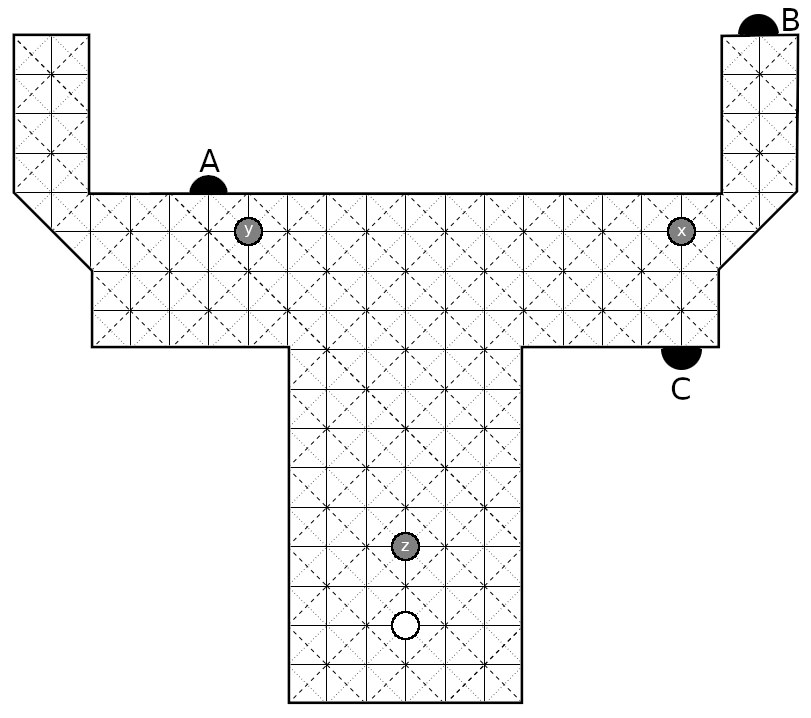
\includegraphics[scale =.9]{assets/Billiards_Puzzle1}
\end{center}

\phChapterWorksheet{Arena 2}{Balls: u, v, w, x, y, z -- Holes: A, B, C, D, E, F}

\begin{center}
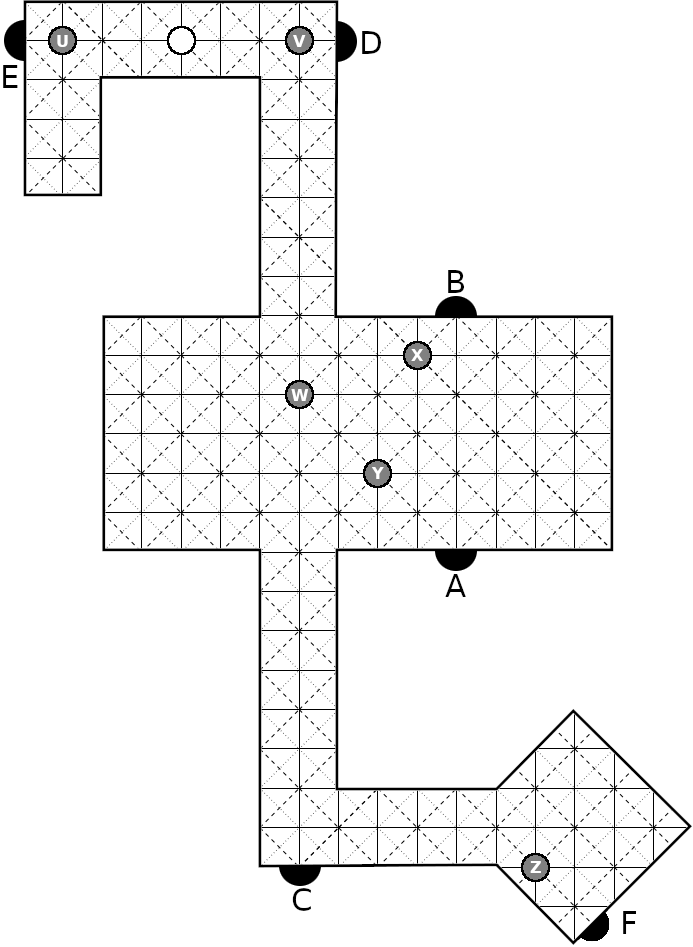
\includegraphics[scale = .8]{assets/Billiards_Puzzle2}
\end{center}

\phChapterWorksheet{Arena 3}{Balls: j, k, l, m, n, h -- Holes: B, C, E, F, G }

\begin{center}
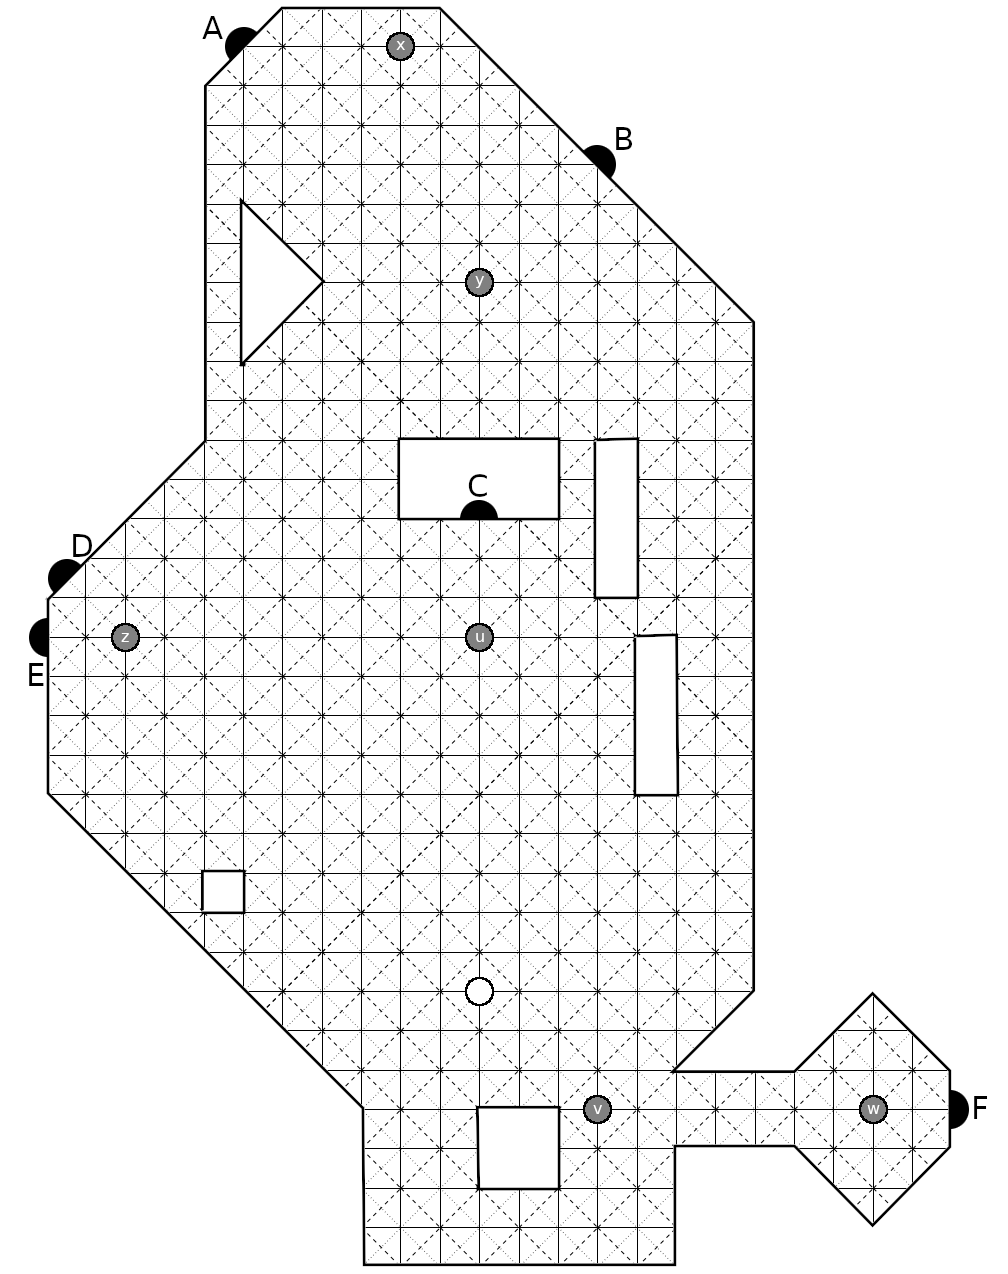
\includegraphics[scale = .6]{assets/Billiards_Puzzle3}
\end{center}

\phChapterWorksheet{Arena 4}{Balls: o, p, t, u -- Holes: A, B, C, D}

\begin{center}
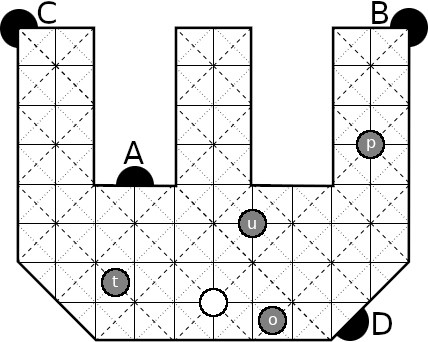
\includegraphics{assets/Billiards_Puzzle4}
\end{center}

\phChapterWorksheet{Journal Page 1}{}

{
  \Large
  \normalfont\wedn
\begin{tabular}{|ccccccc|}
  \hline
  Journal & entry & June & 28, & 1995 & & \\
  \hline
          & & & & & & \\
  \hline
          & Succesful & dig & today. & We & found & a \\
  \hline
  lot & of & pot & shards, & some & with & remarkably \\
  \hline
  intact & artwork. & Like & in & the & tomb, & there \\
  \hline
  are & scenes & of & men & with & circles & around \\
  \hline
  their & heads, & looking & to & the & sky. & We \\
  \hline
  believe & these & represent & past & kings, & deities &, or \\
  \hline
  maybe & both. & I & recall & my & advisor's & words, \\
  \hline
  ``people & are & not & pots.'' & I & should & be \\
  \hline
  careful & before & drawing & any & firm & conclusions. & On \\
  \hline
  the & other & end & of & the & site & from \\
  \hline
  the & tomb & we & found & a & burial & site. \\
  \hline
  It & was & lined & with & red & ochre, & the \\
  \hline
  bodies & were & facing & east & with & their & arms \\
  \hline
  folded. & Already & this & site & has & yielded & so \\
  \hline
  much. & If & only & the & university & understood. & They \\
  \hline
  want & to & save & money & so & badly, & but \\
  \hline
  what & is & it & for & if & not & this? \\
  \hline
\end{tabular}
}

\phChapterWorksheet{Main Puzzle 2}{The Ancient Bazaar}

The Skolem people of Mesopotamia had many myths and legends.
Of great interest to Dr. Jonas was the story of queen Noether, famed for her ability to barter with traders and merchants.
You may have met a good haggler or two in your day, but they didn't have to deal with the strange ways of the Skolem Bazaar.
The Skolem people had no money, instead goods were exchanged for other goods.
Moreover, at the start of each day the shopkeepers would declare their exchange rates.
They were notoriously stubborn and would not change these rates no matter what happened.

Dr. Jonas believed that Noether was real, and wanted to learn as much about her as possible.
Unfortunately, over time every story about Noether split into multiple versions.
In one, Noether entered the marketplace with one bag of spice.
\begin{itemize}
  \item The first shopkeeper declared that 1 bag of spice is equivalent to 4 shell bracelets and 1 clay cup. (\(S \leftrightarrow 4B + C\))
  \item The second shopkeeper declared that 1 shell bracelet is equivalent to 3 bags of spice and 3 clay cups. (\(B \leftrightarrow 3S + 3C\))
  \item The third shopkeeper declared that 1 clay cup is equivalent to 1 bag of spice and 1 shell bracelet. (\(C \leftrightarrow S + B\))    
\end{itemize}
There are two versions of the story:
\begin{enumerate}
  \item Noether entered the bazaar with 1 bag of spice and left with exactly 7 clay cups and nothing else.
  \item Noether entered the bazaar with 1 bag of spice and left with exactly 7 shell bracelets and nothing else.
\end{enumerate}

Dr. Jonas reasoned that the first version was possible and that the second was impossible.
Version one could happen the following way:
\begin{enumerate}
  \item Go to shopkeeper 1: \(S \rightarrow 4B + C\)
  \item Go to shopkeeper 2 and use 1 shell bracelet: \(4B + C = B + 3B + C = 3S + 3C + 3B + C = 3S + 3B + 4C\)
  \item Go to shopkeeper 3 to get a clay cups: \(3S + 3B + 4C = 3C + 4C = 7C\)
  \end{enumerate}
  
%Hint 1:
%So why is the second version impossible? Consider the total amount of bags of spice an clay cups: \(S + C\).
%\begin{itemize}
%  \item The first shopkeeper does not change this amount.
%  \item The second shopkeeper increases/decreases this amount by 6.
%  \item The third shopkeeper does not change this amount.
%\end{itemize}
%Since Noether starts with \(S + C = 1\), it can only become \(1, 7, 13,\) and so on.
%So it is impossible for her to end up with exactly \(7\) bracelets.
%In cluekeeper, this solution would be put in as PI.
%If there were five variants which were possible, impossible, impossible, possible, and impossible, the solution would be PIIPI.

There are many more stories about Noether. If you can figure out which ones are possible and whiche are impossible, you might be able to deciper the mesage hidden in Dr. Jonas' journal.


\phChapterWorksheet{Story 1}{Pomegranates, Fish, and Bread}

\begin{itemize}
\item The first shopkeeper declared that 1 pomegranate is equivalent to 1 fish. (\(P \leftrightarrow F\))
\item The second shopkeeper declared that 1 fish is equivalent to 1 pomegranate, 1 fish, and 1 loaf of bread. (\(F \leftrightarrow P + F + B\))
\item The third shopkeeper declared that 1 loaf of bread is equivalent to 1 pomegranate and 1 fish. (\(B \leftrightarrow P + F\))
\end{itemize}

Label the following versions of the story as possible or impossible.
\begin{enumerate}
\item Noether entered the bazaar with 1 pomegranate and left with 2 pomegranates.
\item Noether entered the bazaar with 1 pomegranate and left with 3 pomegranates.
\item Noether entered the bazaar with 1 pomegranate and left with 3 poomegranates and 1 fish.
\item Noether entered the bazaar with 1 pomegranate and left with 1 loaf of bread.
\item Noether entered the bazaar with 2 pomegranates and left with 2 loaves of bread.
\end{enumerate}


\phChapterWorksheet{Story 2}{Tapestries, Saddles, and Vases}

Story Set-up:
\begin{itemize}
\item The first shopkeeper declared that 1 tapestry is equivalent to 1 saddle and 1 vase. (\(T \leftrightarrow S + V\))
\item The second shopkeeper declared that 1 saddle is equivalent to 1 tapestry and 1 saddle. (\(S \leftrightarrow T + S\))
\item The third shopkeeper declared that 1 vase is equivalent to 1 tapestry and 1 vase. (\(V \leftrightarrow T + V\))
\end{itemize}

Story Versions:
\begin{enumerate}
\item Noether entered the bazaar with 2 tapestries and 1 vase and left with 1 tapestry.
\item Noether entered the bazaar with 1 tapestry and left with 50 tapestries.
\item Noether entered the bazaar with 1 tapestry and left with 1 tapestry and 1 saddle.
\item Noether entered the bazaar with 1 tapestray and left with 1 vase.
\item Noether entered the bazaar with 1 tapestry and left with 3 tapestries.
\end{enumerate}



\phChapterWorksheet{Story 3}{Spice, Vases, and Magic Crystals}

\begin{itemize}
\item The first shopkeeper declared that 1 bag of spice is equivalent to 1 vase. (\(S \leftrightarrow V\))
\item The second shopkeeper declared that 1 vase is equivalent to 1 bag of spice and 1 magic crystal. (\(V \leftrightarrow S + C\))
\item The third shopkeeper declared that 1 magic crystal is worth 2 magic crystals. (\(C \leftrightarrow 2C\))
\end{itemize}

Label the following versions of the story as possible or impossible.
\begin{enumerate}
\item Noether entered the bazaar with 1 bag of spice and left with 2 bags of spice.
\item Noether entered the bazaar with 2 bags of spice and left with 1 bag of spice and 2 vases.
\item Noether entered the bazaar with 3 bags of spice and left with 3 magic crystals.
\item Noether entered the bazaar with 1 bag of spice and left with 1 vase and 2 magic crystals.
\item Noether entered the bazaar with 4 bags of spice and left with 2 bags of spice, 2 vases, and 5 magic crystals.
\end{enumerate}


\phChapterWorksheet{Journal Page 2}{}

To be filled in by Steven.

\phChapterWorksheet{Main Puzzle 3}{Searching the Tombs}

The necropolis of Ramsey is a complex of underground mausoleums, buried by earth and time.
It is also where Dr. Jonas almost got fired.
After finding her first mummy, she seemed to be cursed.
Whenever she entered a new crypt, the mummy inside of it would be as far away from her team as possible.
It's not that they had a hard time finding the mummies, in fact the walls had directions on them leading straight to the sarcophagus.
Still, she had of run of impossibly bad luck.

Once the university realized how much resources Dr. Jonas was spending on her digs, they demanded she stop ``wasting'' their money.
She needed to minimize the number of rooms her team was exploring.
Using ground penetrating radar, Dr. Jonas was able to scout out possible sarcophagus locations and the passages between them.
For instance, one site looked like

\begin{center}
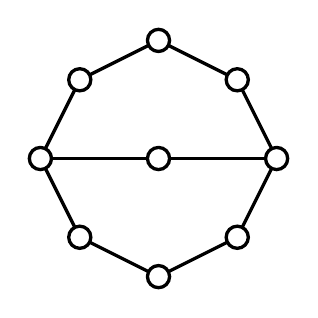
\begin{tikzpicture}[scale=0.5]
    \draw [very thick] (-3,0) -- (3,0);
    \draw [very thick] (-3,0) -- (-2,2) -- (0,3) -- (2,2) -- (3,0) -- (2,-2) -- (0,-3) -- (-2,-2) -- cycle;
    
    \filldraw [color = black, fill = white, very thick] (0,0) circle (8pt);
    \draw [color = black, fill = white, very thick] (-3,0) circle (8pt);
    \draw [color = black, fill = white, very thick] (3,0) circle (8pt);
    \draw [color = black, fill = white, very thick] (0,-3) circle (8pt);
    \draw [color = black, fill = white, very thick] (0,3) circle (8pt);
    \draw [color = black, fill = white, very thick] (2,2) circle (8pt);
    \draw [color = black, fill = white, very thick] (-2,2) circle (8pt);
    \draw [color = black, fill = white, very thick] (2,-2) circle (8pt);
    \draw [color = black, fill = white, very thick] (-2,-2) circle (8pt);
  \end{tikzpicture}
  \end{center}
  
where the circles represent rooms and the lines represent the passages connecting them.

Dr. Jonas could send 9 people out to the site and find the mummy immediately, but that's not very efficient.
Instead, she can send down just 2 people, and have the maximum number of rooms they have to explore be three 3.
Following the Univeristy accounting scheme, this has a cost of 5 as opposed to 9.
This is the best that Dr. Jonas can do.
\begin{center}
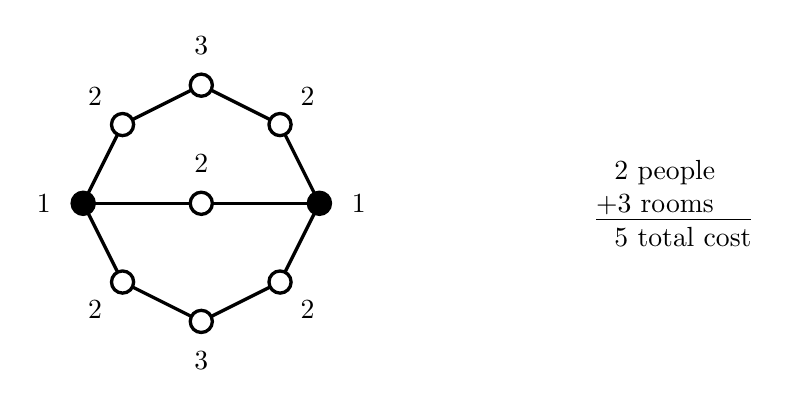
\begin{tikzpicture}[scale=0.5]
    \draw [very thick] (-3,0) -- (3,0);
    \draw [very thick] (-3,0) -- (-2,2) -- (0,3) -- (2,2) -- (3,0) -- (2,-2) -- (0,-3) -- (-2,-2) -- cycle;
    
    \draw [color = black, fill = white, very thick] (0,0) circle (8pt);
    \draw [color = black, fill = black, very thick] (-3,0) circle (8pt);
    \draw [color = black, fill = black, very thick] (3,0) circle (8pt);
    \draw [color = black, fill = white, very thick] (0,-3) circle (8pt);
    \draw [color = black, fill = white, very thick] (0,3) circle (8pt);
    \draw [color = black, fill = white, very thick] (2,2) circle (8pt);
    \draw [color = black, fill = white, very thick] (-2,2) circle (8pt);
    \draw [color = black, fill = white, very thick] (2,-2) circle (8pt);
    \draw [color = black, fill = white, very thick] (-2,-2) circle (8pt);

    \node at (0,1) {2};
    \node at (-4,0) {1};
    \node at (4,0) {1};
    \node at (0,-4) {3};
    \node at (2.7,2.7) {2};
    \node at (-2.7,2.7) {2};
    \node at (2.7,-2.7) {2};
    \node at (-2.7,-2.7) {2};
    \node at (0,4) {3};

    \node[align=left] at (12,0) {\,\, 2 people \\ \underline{+3 rooms \quad} \\ \,\, 5 total cost};
    
\end{tikzpicture}
\end{center}

There are four more site diagrams in Dr. Jonas' notes.
If you can figure out the minimum cost of exploring these crypts, B. Fraiser will be able to tell you how to deciper the next journal page.


\phChapterWorksheet{Site 1}{}

\begin{center}
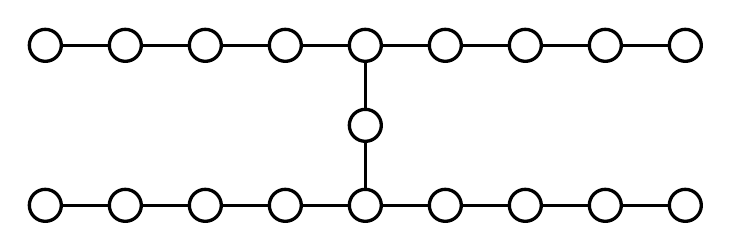
\begin{tikzpicture}[x=0.2in,y=0.2in]
  \draw [very thick] (-8,2) -- (-6,2) -- (-4,2) -- (-2,2) -- (0,2) -- (2,2) -- (4,2) -- (6,2) -- (8,2);
  \draw [very thick] (-8,-2) -- (-6,-2) -- (-4,-2) -- (-2,-2) -- (0,-2) -- (2,-2) -- (4,-2) -- (6,-2) -- (8,-2);
  \draw [very thick] (0,2) -- (0,-2);
    
    \draw [color = black, fill = white, very thick] (-8,2) circle (0.4);
    \draw [color = black, fill = white, very thick] (-6,2) circle (0.4);
    \draw [color = black, fill = white, very thick] (-4,2) circle (0.4);
    \draw [color = black, fill = white, very thick] (-2,2) circle (0.4);
    \draw [color = black, fill = white, very thick] (0,2) circle (0.4);
    \draw [color = black, fill = white, very thick] (2,2) circle (0.4);
    \draw [color = black, fill = white, very thick] (4,2) circle (0.4);
    \draw [color = black, fill = white, very thick] (6,2) circle (0.4);
    \draw [color = black, fill = white, very thick] (8,2) circle (0.4);

    \draw [color = black, fill = white, very thick] (-8,-2) circle (0.4);
    \draw [color = black, fill = white, very thick] (-6,-2) circle (0.4);
    \draw [color = black, fill = white, very thick] (-4,-2) circle (0.4);
    \draw [color = black, fill = white, very thick] (-2,-2) circle (0.4);
    \draw [color = black, fill = white, very thick] (0,-2) circle (0.4);
    \draw [color = black, fill = white, very thick] (2,-2) circle (0.4);
    \draw [color = black, fill = white, very thick] (4,-2) circle (0.4);
    \draw [color = black, fill = white, very thick] (6,-2) circle (0.4);
    \draw [color = black, fill = white, very thick] (8,-2) circle (0.4);

    \draw [color = black, fill = white, very thick] (0,0) circle (0.4);
  \end{tikzpicture}

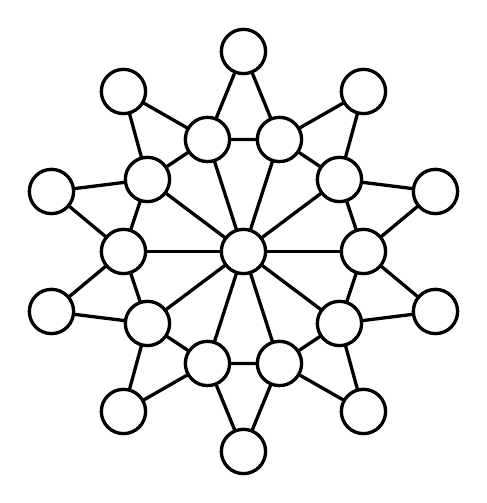
\begin{tikzpicture}[x=0.2in,y=0.2in]
    \draw [very thick] (-3,0) -- (3,0);
    \draw [very thick] (-2.4,1.8) -- (2.4,-1.8);
    \draw [very thick] (-.9,2.8) -- (.9,-2.8);
    \draw [very thick] (.9,2.8) -- (-.9,-2.8);
    \draw [very thick] (2.4,1.8) -- (-2.4,-1.8);
    \draw [very thick] (-3,0) -- (-2.4,1.8) -- (-.9,2.8) -- (.9,2.8) -- (2.4,1.8) -- (3,0) -- (2.4,-1.8) -- (.9,-2.8) -- (-.9,-2.8) -- (-2.4,-1.8) -- (-3,0);
    \draw [very thick] (-3,0) -- (-4.8,1.5) -- (-2.4,1.8) -- (-3,4) -- (-.9,2.8) -- (0,5) -- (.9,2.8) -- (3,4) -- (2.4,1.8) -- (4.8,1.5) -- (3,0) -- (4.8,-1.5) -- (2.4,-1.8) -- (3,-4) -- (.9,-2.8) -- (0,-5) -- (-.9, -2.8) -- (-3,-4) -- (-2.4,-1.8) -- (-4.8,-1.5) -- (-3,0);
    
    \draw [color = black, fill = white, very thick] (0,0) circle (8pt);
    \draw [color = black, fill = white, very thick] (-3,0) circle (8pt);
    \draw [color = black, fill = white, very thick] (-2.4,1.8) circle (8pt);
    \draw [color = black, fill = white, very thick] (-.9,2.8) circle (8pt);
    \draw [color = black, fill = white, very thick] (.9,2.8) circle (8pt);
    \draw [color = black, fill = white, very thick] (2.4,1.8) circle (8pt);
    \draw [color = black, fill = white, very thick] (3,0) circle (8pt);
    \draw [color = black, fill = white, very thick] (2.4,-1.8) circle (8pt);
    \draw [color = black, fill = white, very thick] (.9,-2.8) circle (8pt);
    \draw [color = black, fill = white, very thick] (-.9,-2.8) circle (8pt);
    \draw [color = black, fill = white, very thick] (-2.4,-1.8) circle (8pt);
    \draw [color = black, fill = white, very thick] (-4.8,1.5) circle (8pt);
    \draw [color = black, fill = white, very thick] (-3,4) circle (8pt);
    \draw [color = black, fill = white, very thick] (0,5) circle (8pt);
    \draw [color = black, fill = white, very thick] (3,4) circle (8pt);
    \draw [color = black, fill = white, very thick] (4.8,1.5) circle (8pt);
    \draw [color = black, fill = white, very thick] (4.8,-1.5) circle (8pt);
    \draw [color = black, fill = white, very thick] (3,-4) circle (8pt);
    \draw [color = black, fill = white, very thick] (0,-5) circle (8pt);
    \draw [color = black, fill = white, very thick] (-3,-4) circle (8pt);
    \draw [color = black, fill = white, very thick] (-4.8,-1.5) circle (8pt);
  \end{tikzpicture}

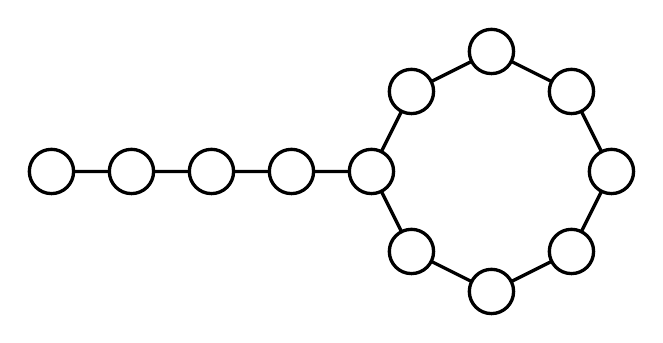
\begin{tikzpicture}[x=0.2in,y=0.2in]
    \draw [very thick] (-11,0) -- (-9,0) -- (-7,0) -- (-5,0) -- (-3,0) -- (-2,2) -- (0,3) -- (2,2) -- (3,0) -- (2,-2) -- (0,-3) -- (-2,-2) -- (-3,0);
    
    \draw [color = black, fill = white, very thick] (-11,0) circle (8pt);
    \draw [color = black, fill = white, very thick] (-9,0) circle (8pt);
    \draw [color = black, fill = white, very thick] (-7,0) circle (8pt);
    \draw [color = black, fill = white, very thick] (-5,0) circle (8pt);
    \draw [color = black, fill = white, very thick] (-3,0) circle (8pt);
    \draw [color = black, fill = white, very thick] (3,0) circle (8pt);
    \draw [color = black, fill = white, very thick] (0,-3) circle (8pt);
    \draw [color = black, fill = white, very thick] (0,3) circle (8pt);
    \draw [color = black, fill = white, very thick] (2,2) circle (8pt);
    \draw [color = black, fill = white, very thick] (-2,2) circle (8pt);
    \draw [color = black, fill = white, very thick] (2,-2) circle (8pt);
    \draw [color = black, fill = white, very thick] (-2,-2) circle (8pt);
  \end{tikzpicture}

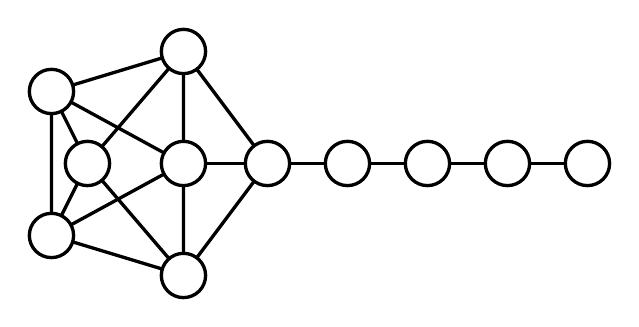
\begin{tikzpicture}[x=0.2in,y=0.2in]
    \draw [very thick] (.9,0) -- (3,0) -- (5,0) -- (7,0) -- (9,0) -- (11,0);
    \draw [very thick] (.9, 2.8) -- (.9,-2.8) -- (-1.5,0) -- cycle;
    \draw [very thick] (-2.4, 1.8) -- (.9,0) -- (-2.4, -1.8) -- (-1.5,0) -- cycle;
    \draw [very thick] (-2.4,1.8) -- (.9,2.8) -- (3,0) -- (.9,-2.8) -- (-2.4,-1.8) -- cycle;
    
    \draw [color = black, fill = white, very thick] (11,0) circle (8pt);
    \draw [color = black, fill = white, very thick] (9,0) circle (8pt);
    \draw [color = black, fill = white, very thick] (7,0) circle (8pt);
    \draw [color = black, fill = white, very thick] (5,0) circle (8pt);
    \draw [color = black, fill = white, very thick] (-2.4,1.8) circle (8pt);
    \draw [color = black, fill = white, very thick] (.9,2.8) circle (8pt);
    \draw [color = black, fill = white, very thick] (3,0) circle (8pt);
    \draw [color = black, fill = white, very thick] (.9,-2.8) circle (8pt);
    \draw [color = black, fill = white, very thick] (-2.4,-1.8) circle (8pt);
    \draw [color = black, fill = white, very thick] (.9,0) circle (8pt);
    \draw [color = black, fill = white, very thick] (-1.5,0) circle (8pt);
  \end{tikzpicture}
  \end{center}


\phChapterWorksheet{Site 2}{}

\begin{center}
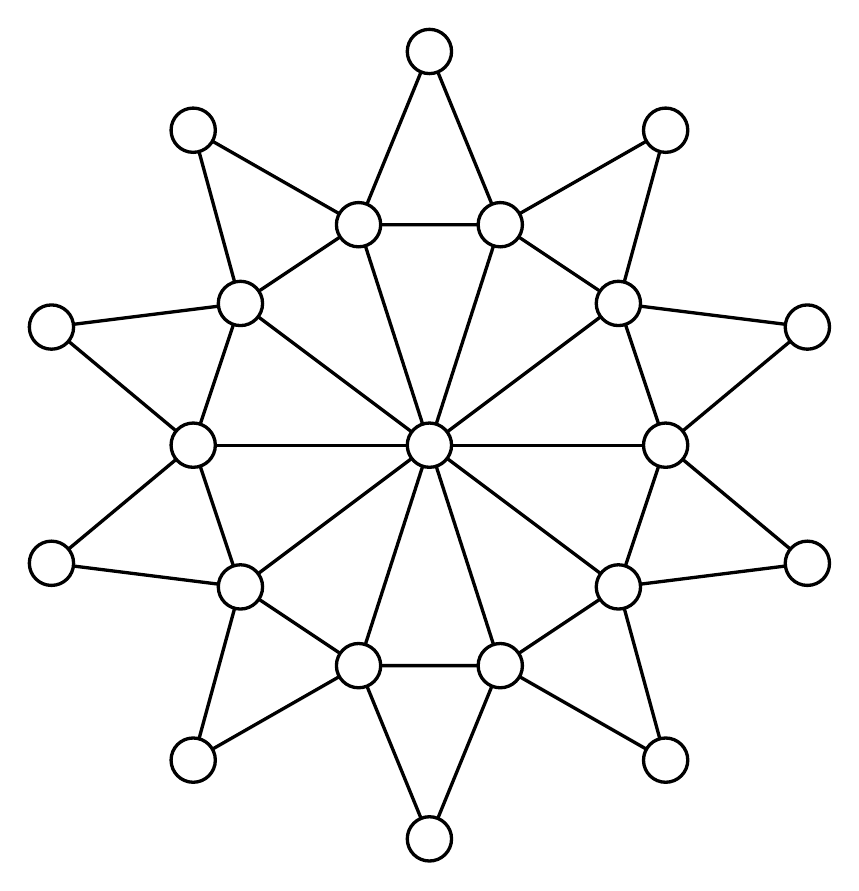
\begin{tikzpicture}
    \draw [very thick] (-3,0) -- (3,0);
    \draw [very thick] (-2.4,1.8) -- (2.4,-1.8);
    \draw [very thick] (-.9,2.8) -- (.9,-2.8);
    \draw [very thick] (.9,2.8) -- (-.9,-2.8);
    \draw [very thick] (2.4,1.8) -- (-2.4,-1.8);
    \draw [very thick] (-3,0) -- (-2.4,1.8) -- (-.9,2.8) -- (.9,2.8) -- (2.4,1.8) -- (3,0) -- (2.4,-1.8) -- (.9,-2.8) -- (-.9,-2.8) -- (-2.4,-1.8) -- (-3,0);
    \draw [very thick] (-3,0) -- (-4.8,1.5) -- (-2.4,1.8) -- (-3,4) -- (-.9,2.8) -- (0,5) -- (.9,2.8) -- (3,4) -- (2.4,1.8) -- (4.8,1.5) -- (3,0) -- (4.8,-1.5) -- (2.4,-1.8) -- (3,-4) -- (.9,-2.8) -- (0,-5) -- (-.9, -2.8) -- (-3,-4) -- (-2.4,-1.8) -- (-4.8,-1.5) -- (-3,0);
    
    \draw [color = black, fill = white, very thick] (0,0) circle (8pt);
    \draw [color = black, fill = white, very thick] (-3,0) circle (8pt);
    \draw [color = black, fill = white, very thick] (-2.4,1.8) circle (8pt);
    \draw [color = black, fill = white, very thick] (-.9,2.8) circle (8pt);
    \draw [color = black, fill = white, very thick] (.9,2.8) circle (8pt);
    \draw [color = black, fill = white, very thick] (2.4,1.8) circle (8pt);
    \draw [color = black, fill = white, very thick] (3,0) circle (8pt);
    \draw [color = black, fill = white, very thick] (2.4,-1.8) circle (8pt);
    \draw [color = black, fill = white, very thick] (.9,-2.8) circle (8pt);
    \draw [color = black, fill = white, very thick] (-.9,-2.8) circle (8pt);
    \draw [color = black, fill = white, very thick] (-2.4,-1.8) circle (8pt);
    \draw [color = black, fill = white, very thick] (-4.8,1.5) circle (8pt);
    \draw [color = black, fill = white, very thick] (-3,4) circle (8pt);
    \draw [color = black, fill = white, very thick] (0,5) circle (8pt);
    \draw [color = black, fill = white, very thick] (3,4) circle (8pt);
    \draw [color = black, fill = white, very thick] (4.8,1.5) circle (8pt);
    \draw [color = black, fill = white, very thick] (4.8,-1.5) circle (8pt);
    \draw [color = black, fill = white, very thick] (3,-4) circle (8pt);
    \draw [color = black, fill = white, very thick] (0,-5) circle (8pt);
    \draw [color = black, fill = white, very thick] (-3,-4) circle (8pt);
    \draw [color = black, fill = white, very thick] (-4.8,-1.5) circle (8pt);
  \end{tikzpicture}
  \end{center}

\phChapterWorksheet{Site 3}{}

\begin{center}
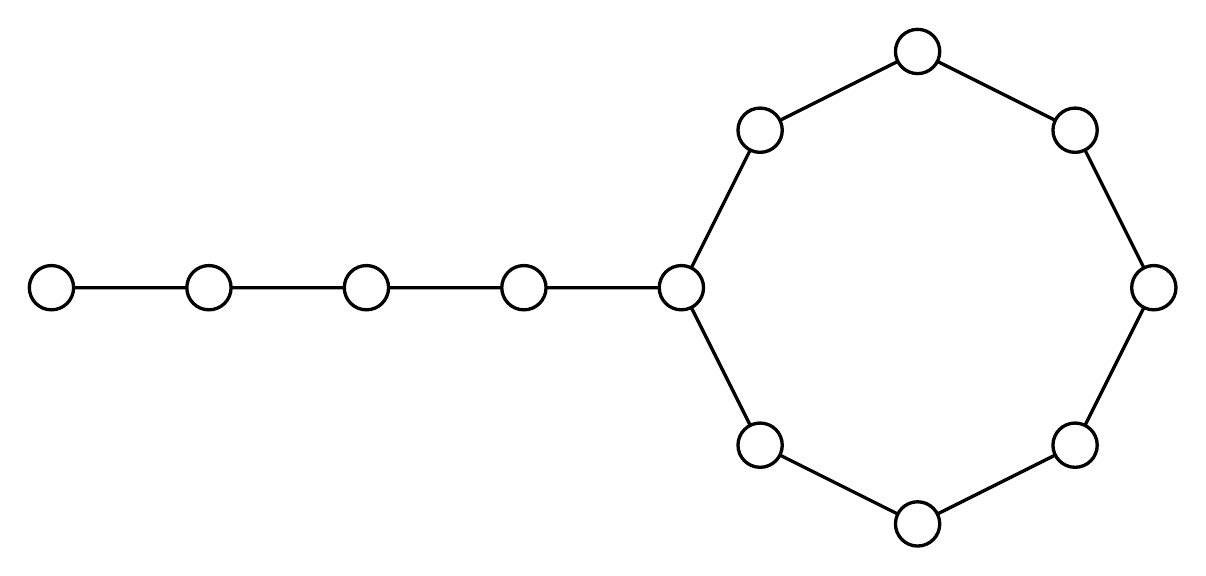
\begin{tikzpicture}
    \draw [very thick] (-11,0) -- (-9,0) -- (-7,0) -- (-5,0) -- (-3,0) -- (-2,2) -- (0,3) -- (2,2) -- (3,0) -- (2,-2) -- (0,-3) -- (-2,-2) -- (-3,0);
    
    \draw [color = black, fill = white, very thick] (-11,0) circle (8pt);
    \draw [color = black, fill = white, very thick] (-9,0) circle (8pt);
    \draw [color = black, fill = white, very thick] (-7,0) circle (8pt);
    \draw [color = black, fill = white, very thick] (-5,0) circle (8pt);
    \draw [color = black, fill = white, very thick] (-3,0) circle (8pt);
    \draw [color = black, fill = white, very thick] (3,0) circle (8pt);
    \draw [color = black, fill = white, very thick] (0,-3) circle (8pt);
    \draw [color = black, fill = white, very thick] (0,3) circle (8pt);
    \draw [color = black, fill = white, very thick] (2,2) circle (8pt);
    \draw [color = black, fill = white, very thick] (-2,2) circle (8pt);
    \draw [color = black, fill = white, very thick] (2,-2) circle (8pt);
    \draw [color = black, fill = white, very thick] (-2,-2) circle (8pt);
  \end{tikzpicture}
\end{center}
  

\phChapterWorksheet{Site 4}{}

\begin{center}
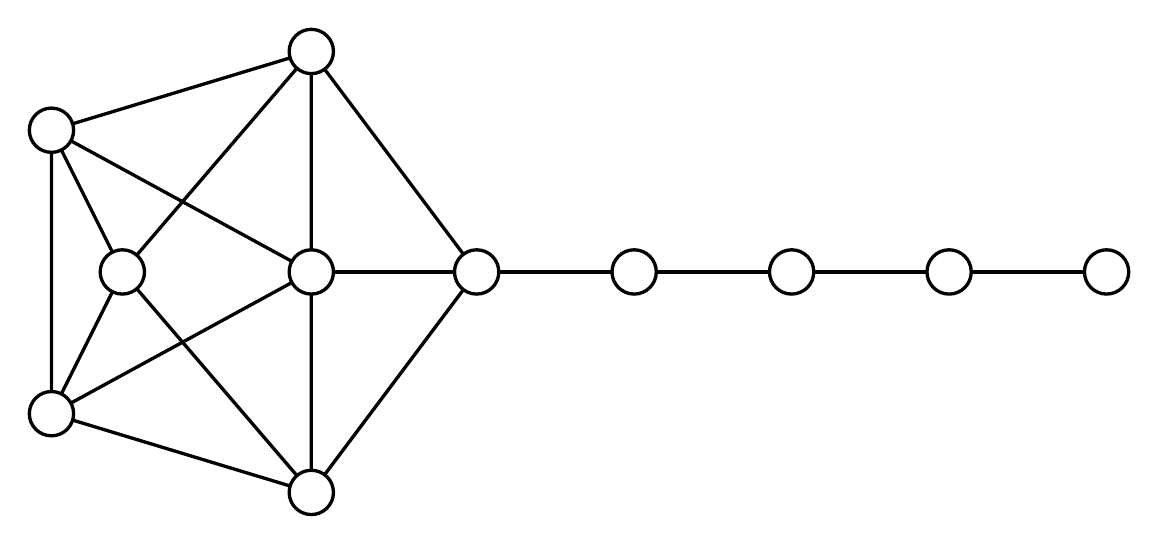
\begin{tikzpicture}
    \draw [very thick] (.9,0) -- (3,0) -- (5,0) -- (7,0) -- (9,0) -- (11,0);
    \draw [very thick] (.9, 2.8) -- (.9,-2.8) -- (-1.5,0) -- cycle;
    \draw [very thick] (-2.4, 1.8) -- (.9,0) -- (-2.4, -1.8) -- (-1.5,0) -- cycle;
    \draw [very thick] (-2.4,1.8) -- (.9,2.8) -- (3,0) -- (.9,-2.8) -- (-2.4,-1.8) -- cycle;
    
    \draw [color = black, fill = white, very thick] (11,0) circle (8pt);
    \draw [color = black, fill = white, very thick] (9,0) circle (8pt);
    \draw [color = black, fill = white, very thick] (7,0) circle (8pt);
    \draw [color = black, fill = white, very thick] (5,0) circle (8pt);
    \draw [color = black, fill = white, very thick] (-2.4,1.8) circle (8pt);
    \draw [color = black, fill = white, very thick] (.9,2.8) circle (8pt);
    \draw [color = black, fill = white, very thick] (3,0) circle (8pt);
    \draw [color = black, fill = white, very thick] (.9,-2.8) circle (8pt);
    \draw [color = black, fill = white, very thick] (-2.4,-1.8) circle (8pt);
    \draw [color = black, fill = white, very thick] (.9,0) circle (8pt);
    \draw [color = black, fill = white, very thick] (-1.5,0) circle (8pt);
  \end{tikzpicture}
  \end{center}

\phChapterWorksheet{Journal Page 3}{}

\begin{tikzpicture}
\draw[-latex] (0,0) -- (15,0);
\draw[-latex] (0,0) -- (0,15);
\foreach \x in {1,2,...,14} {
  \draw (\x,0.1) -- (\x,-0.1);
  \draw (-0.1,\x) -- (0.1,\x);
}
%\draw (2,3) -- (10,6) -- (11,11) -- (3,10) -- (2,3);
\node at (12,3) {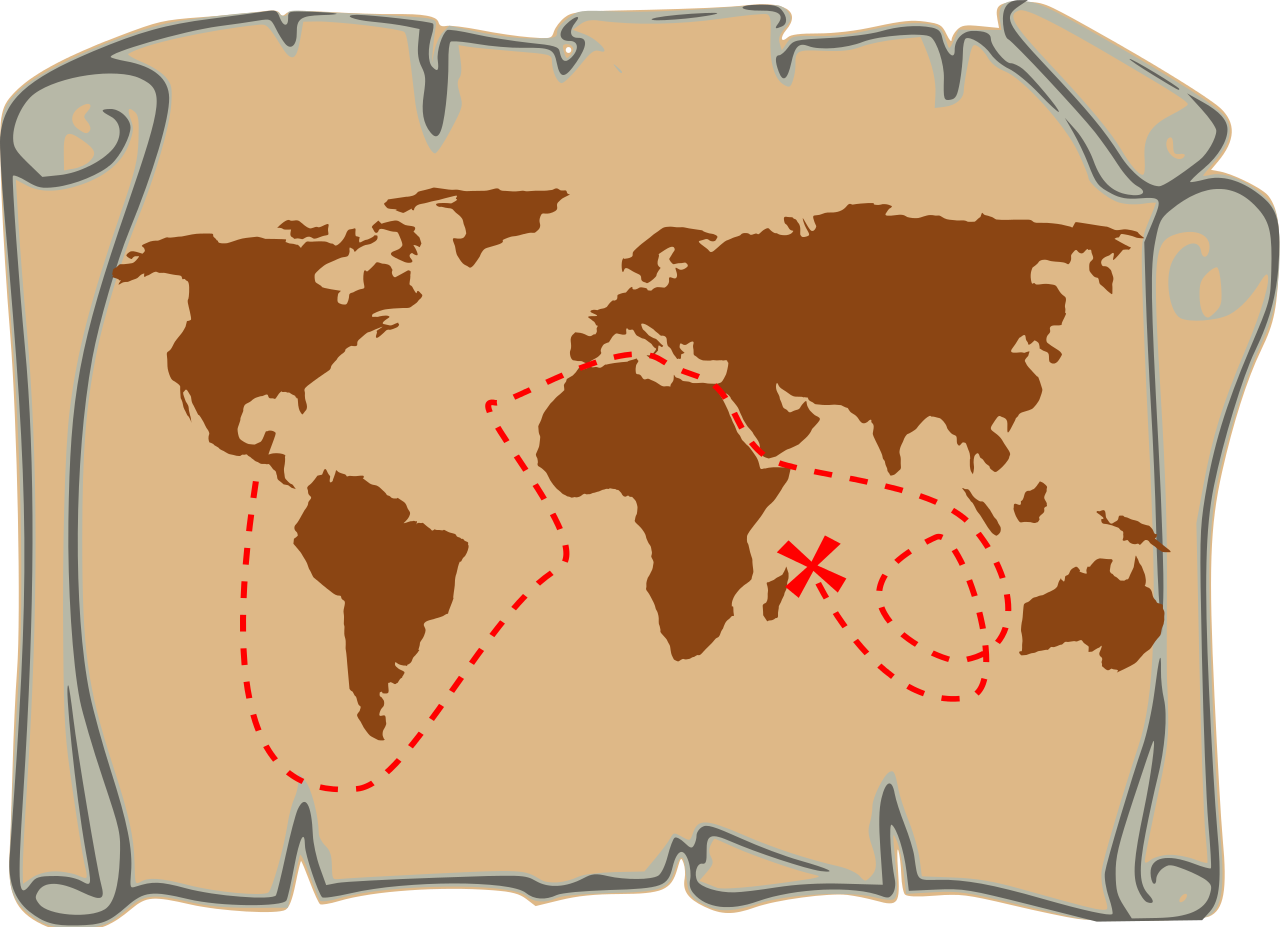
\includegraphics[width=1in]{assets/clipart/map.png}};
\node at (4,6) {
\includegraphics[width=1in]{assets/clipart/hat.png}};
\node at (8,8) {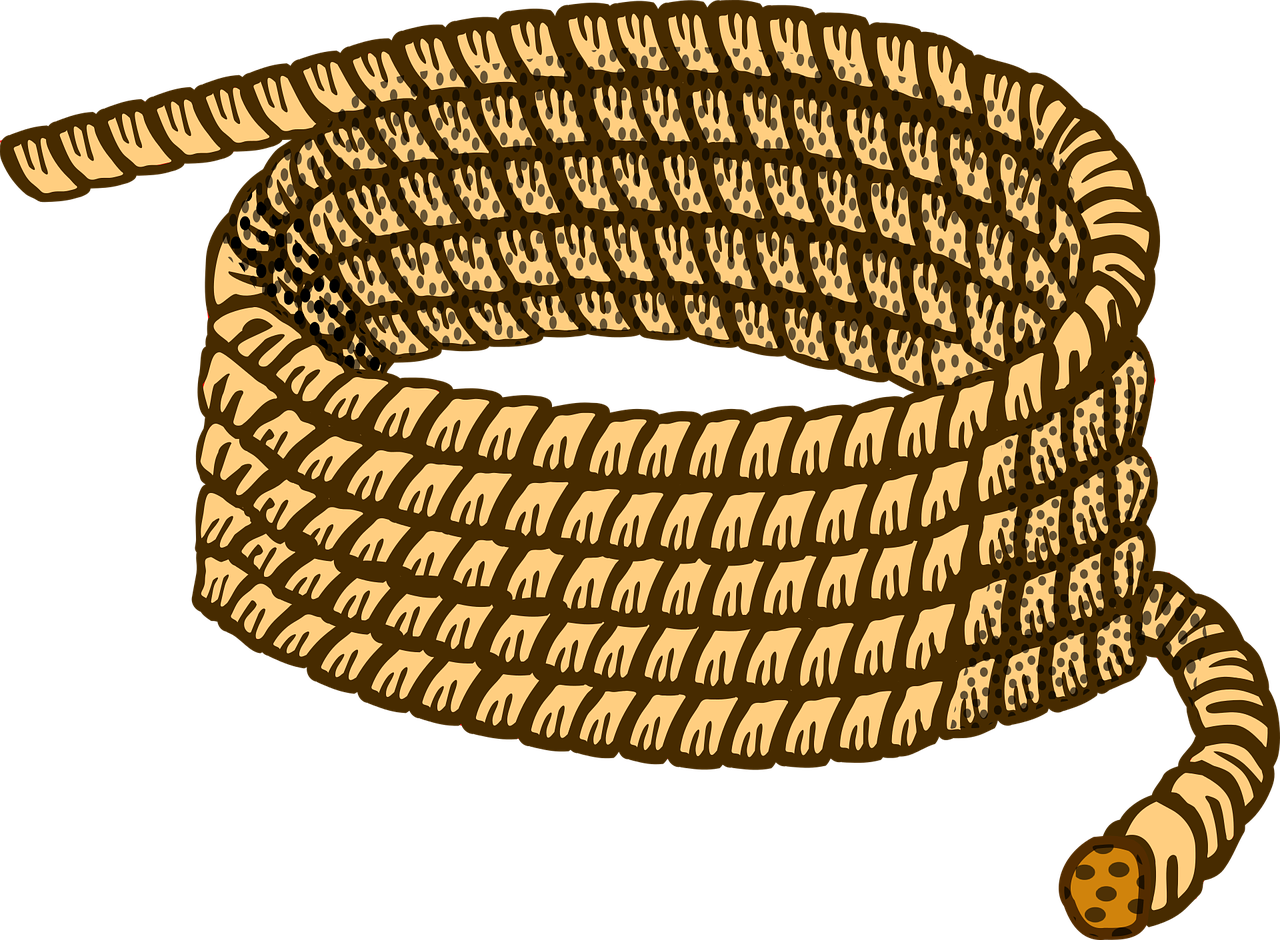
\includegraphics[width=1in]{assets/clipart/rope.png}};
\node at (3,12) {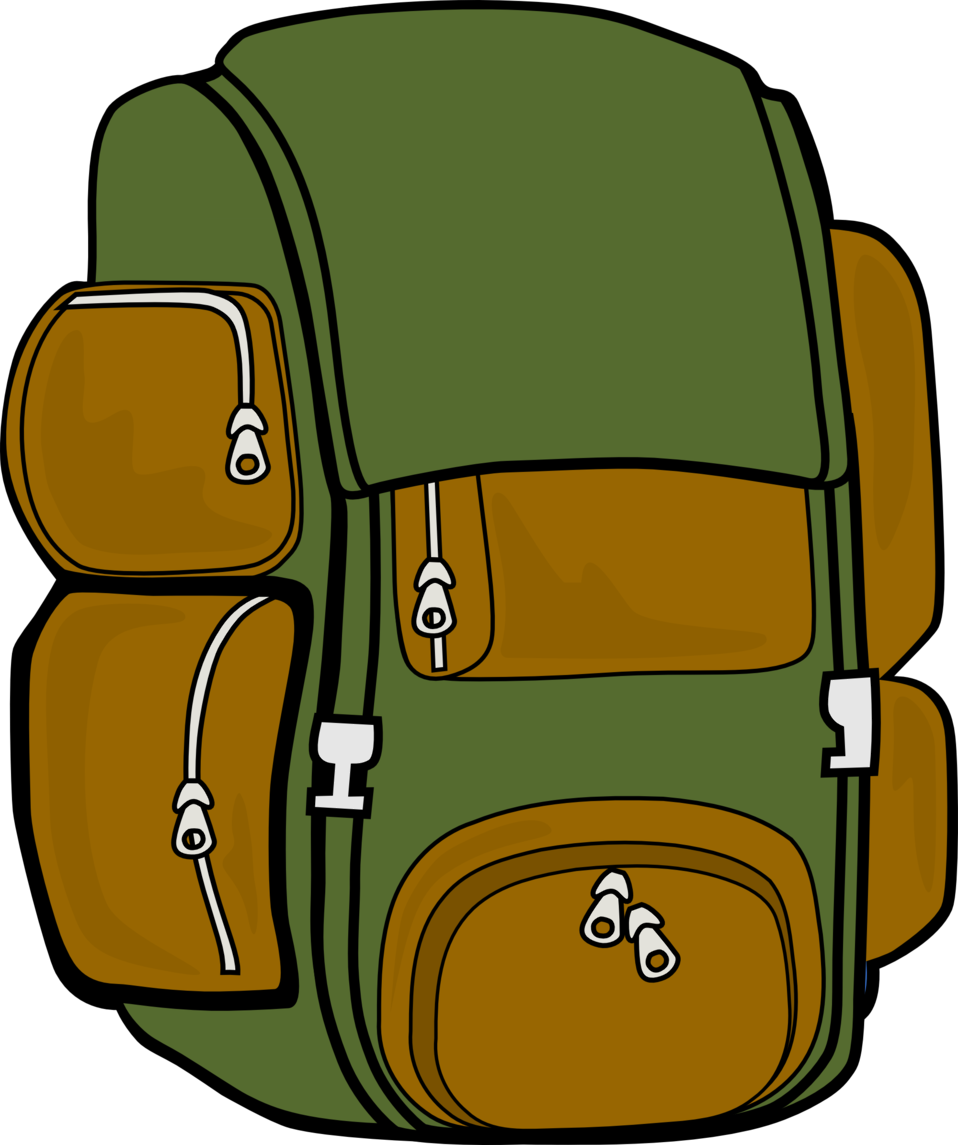
\includegraphics[width=1in]{assets/clipart/backpack.png}};
\node at (13,7) {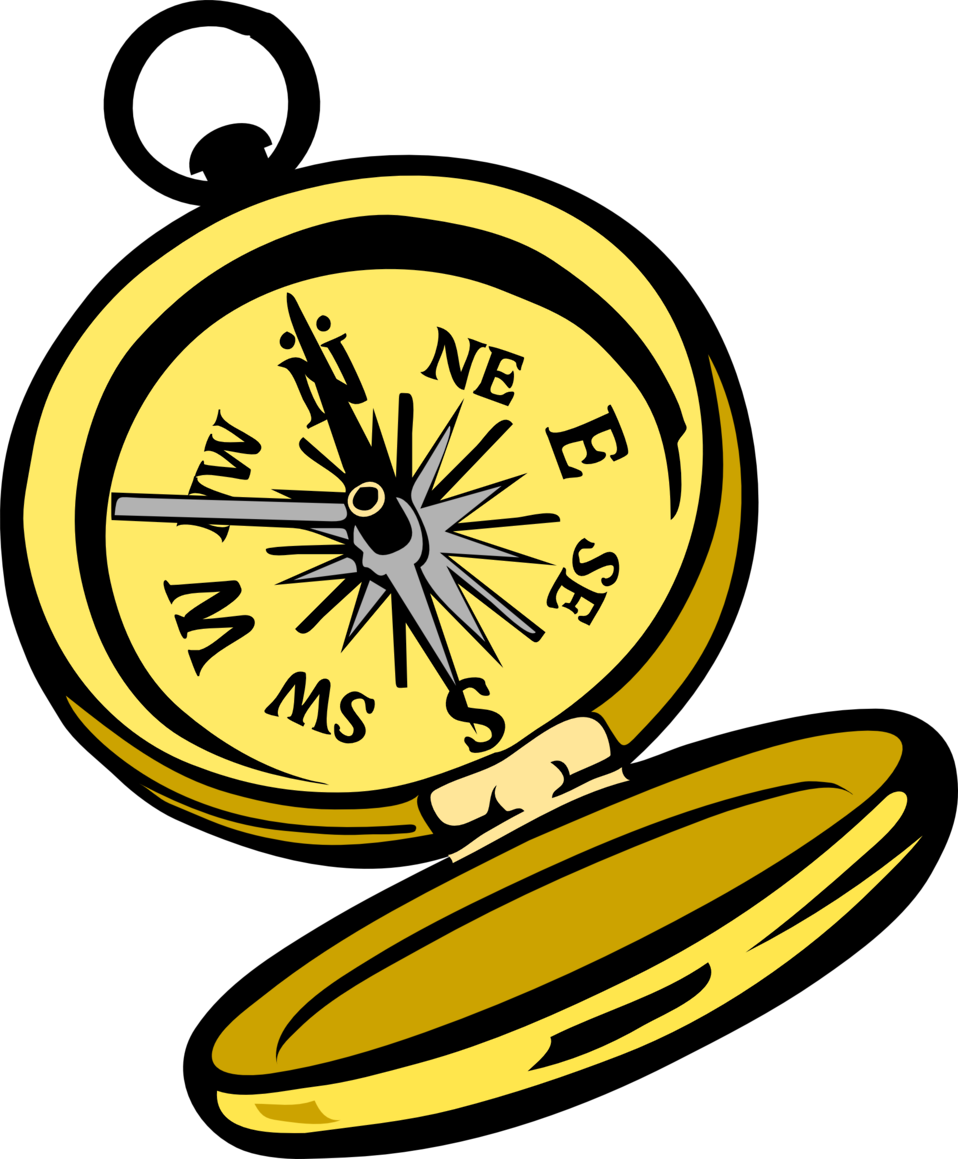
\includegraphics[width=1in]{assets/clipart/compass.png}};
\node at (7,2) {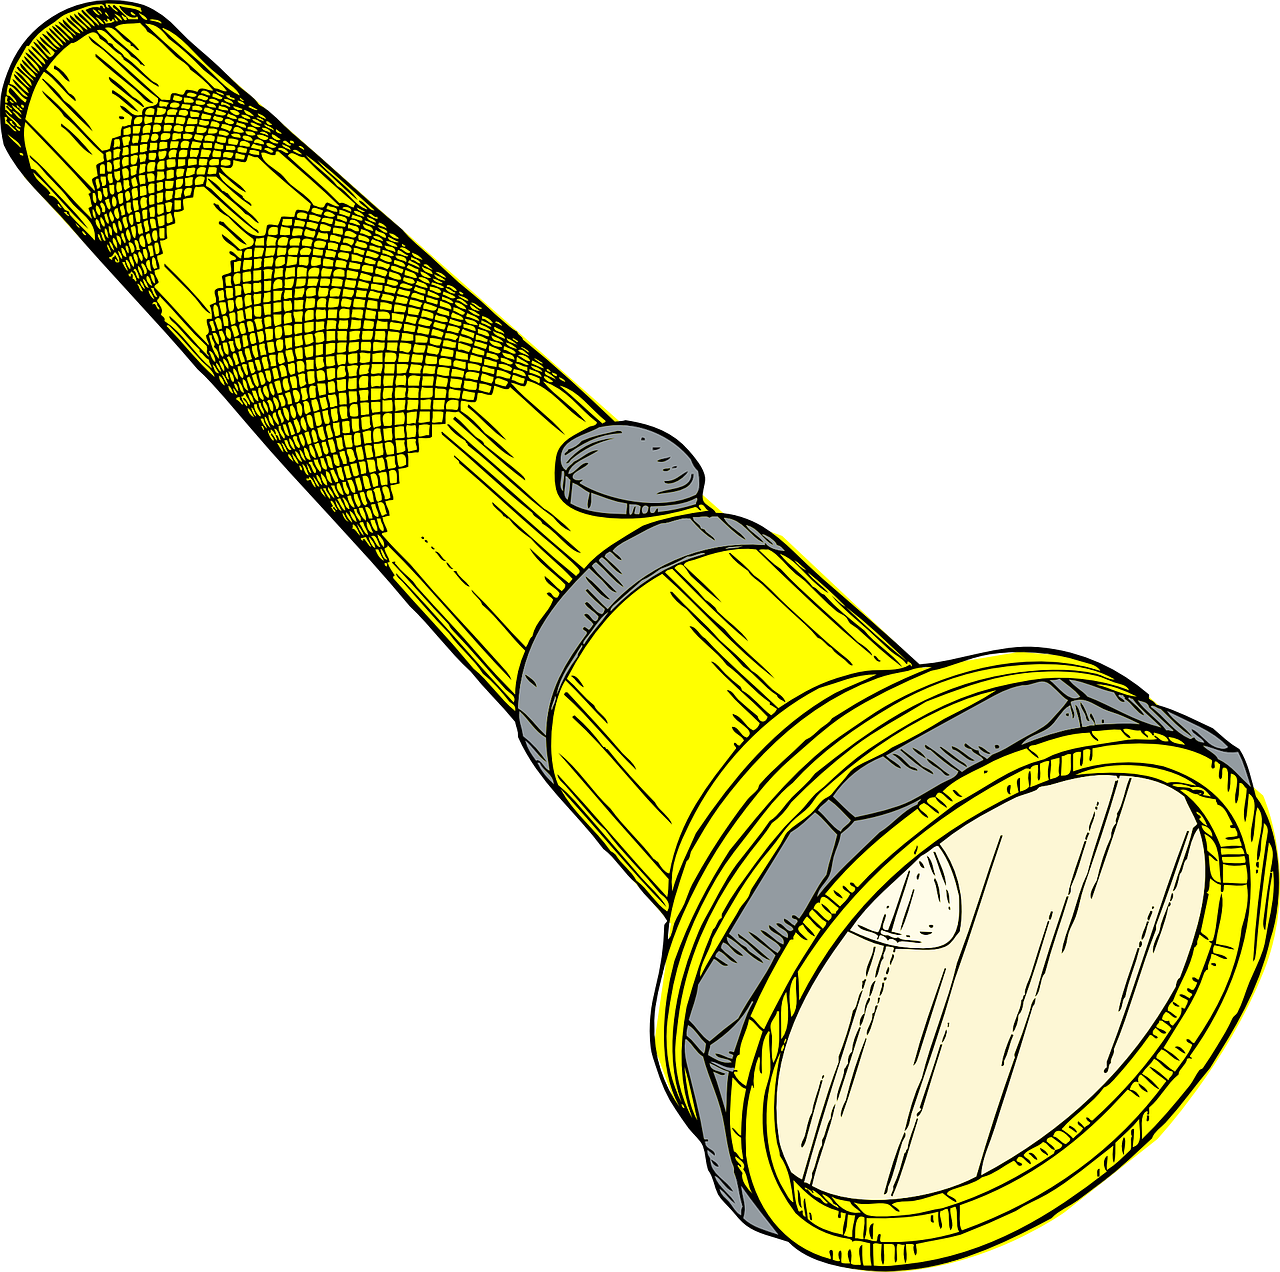
\includegraphics[width=1in]{assets/clipart/flashlight.png}};
\end{tikzpicture}

\vfill
Site Adjustment:
\begin{enumerate}
\item Site 1: \((?,?) + (-4,-16)\)
\item Site 2: \((?,?) + (6,-15)\)
\item Site 3: \((?,?) + (5,-1)\)
\item Site 4: \((?,?) + (-3,-1)\)
\end{enumerate}

\vfill

\phChapterWorksheet{Main Puzzle 4}{Ancient Gerrymandering}

One of Dr. Jonas' greatest discoveries was the democratic nation
of Heyting people, who kept meticulous records of their elections 
and their rulers.
Strangely, even though the Heyting people were democratic, 
their voting records indicated that many of their elected officials
recived far less than the majority of the votes.
How could this happen?

Well, to simplify the voting process, each of the Heyting tribes had broken their 
land up into districts.
Each district had one vote for the next ruler of that tribe, which was based upon
the majority vote from within the district.
However, since the existing tribe leaders were allowed to draw the boundaries 
of the districts as long as they respected the following guidelines,
the minority party X was able to keep power from the majority party O.
\begin{enumerate}
\item Each district had to be a single connected region.
\item Each district needed to contain a single temple (marked as stars on the maps).
\item The difference in population between any two districts had to be 5 or less.
\item All district boundary lines had to follow the horizontal and vertical grid lines provided.
\end{enumerate}

For each of the four tribes, find a way to draw the district lines such that party X
has strictly more votes than party O in more than half of the total districts.
Then enter the total population (Xs and Os) for each of the capital districts (containing
the biggest star) into
ClueKeeper using the following format: \texttt{A\#\#-B\#\#-C\#\#-D\#\#}.

I'm attaching an example Tribe X. Note that its solution would be entered into ClueKeeper as \texttt{X19}. -BF

\hfill
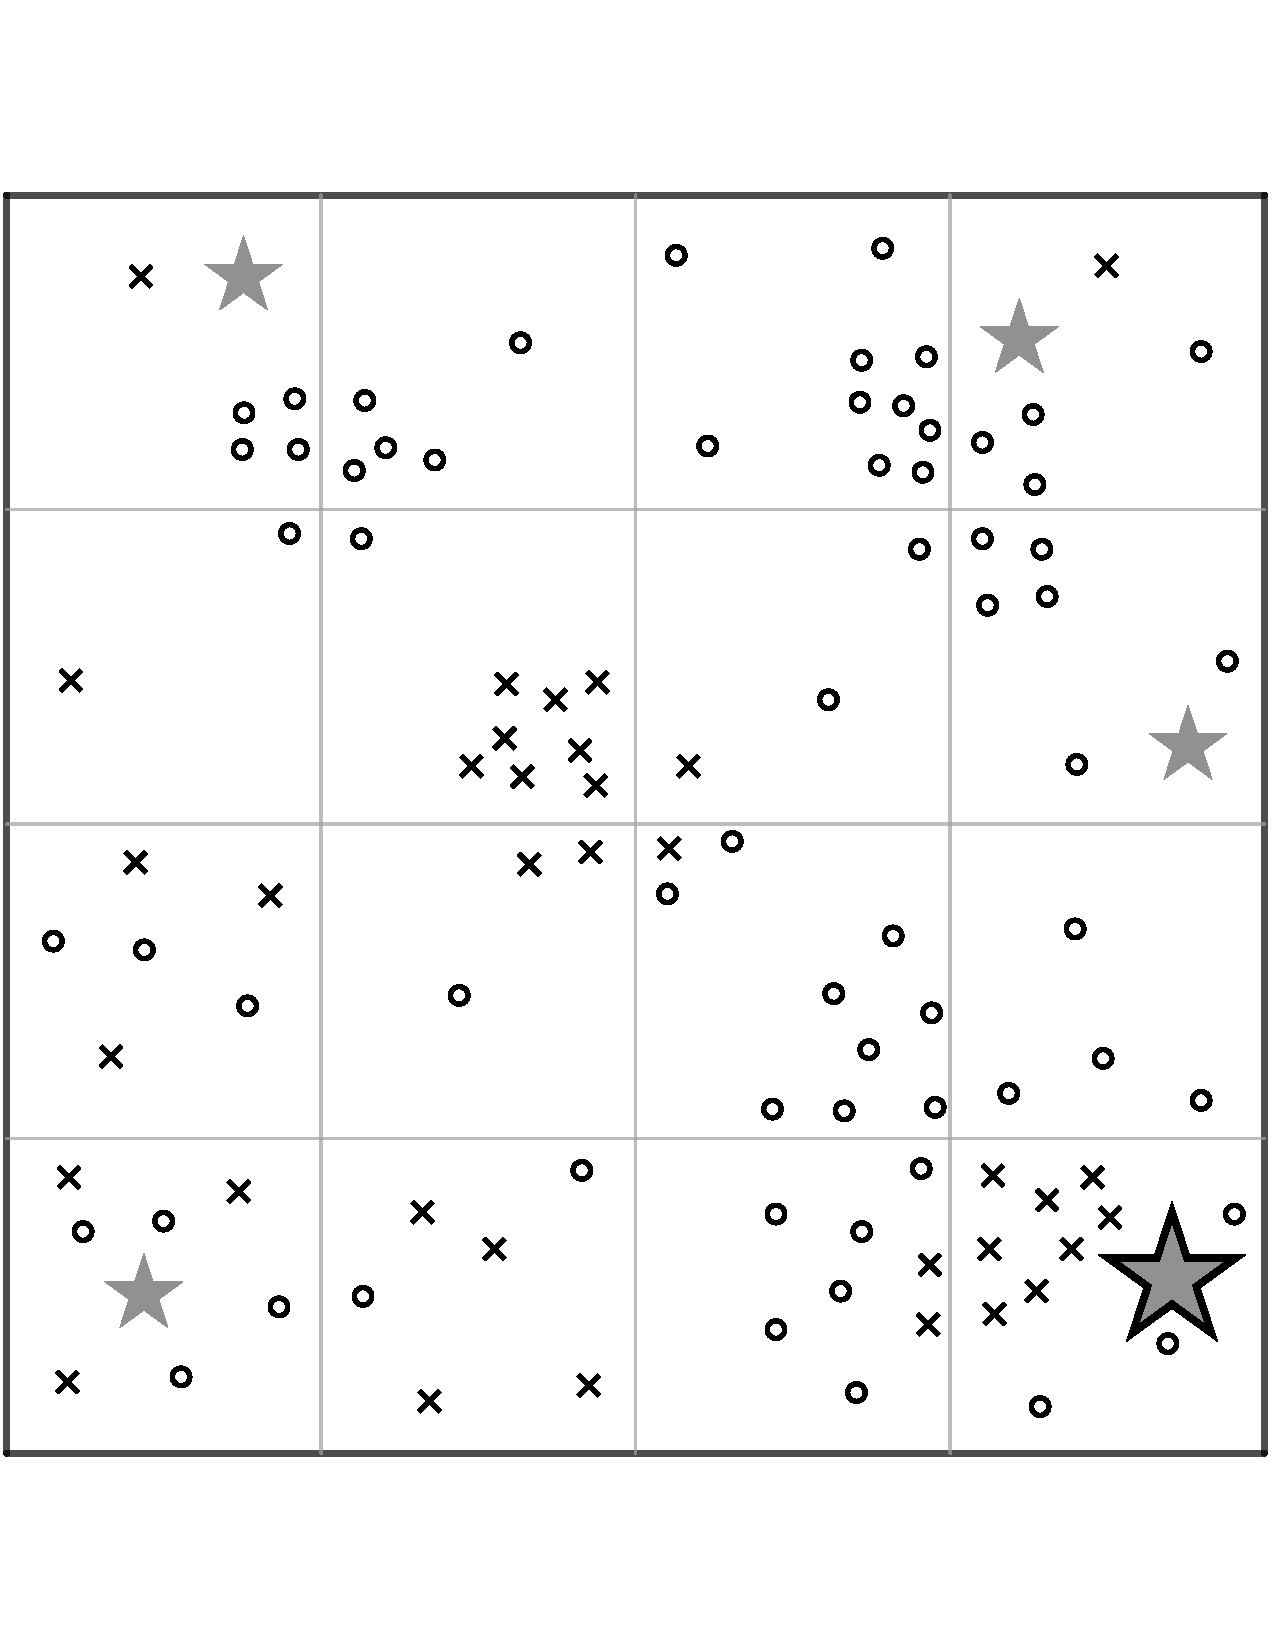
\includegraphics[width=2.5in]{assets/gerrymander-example.pdf} 
\hfill
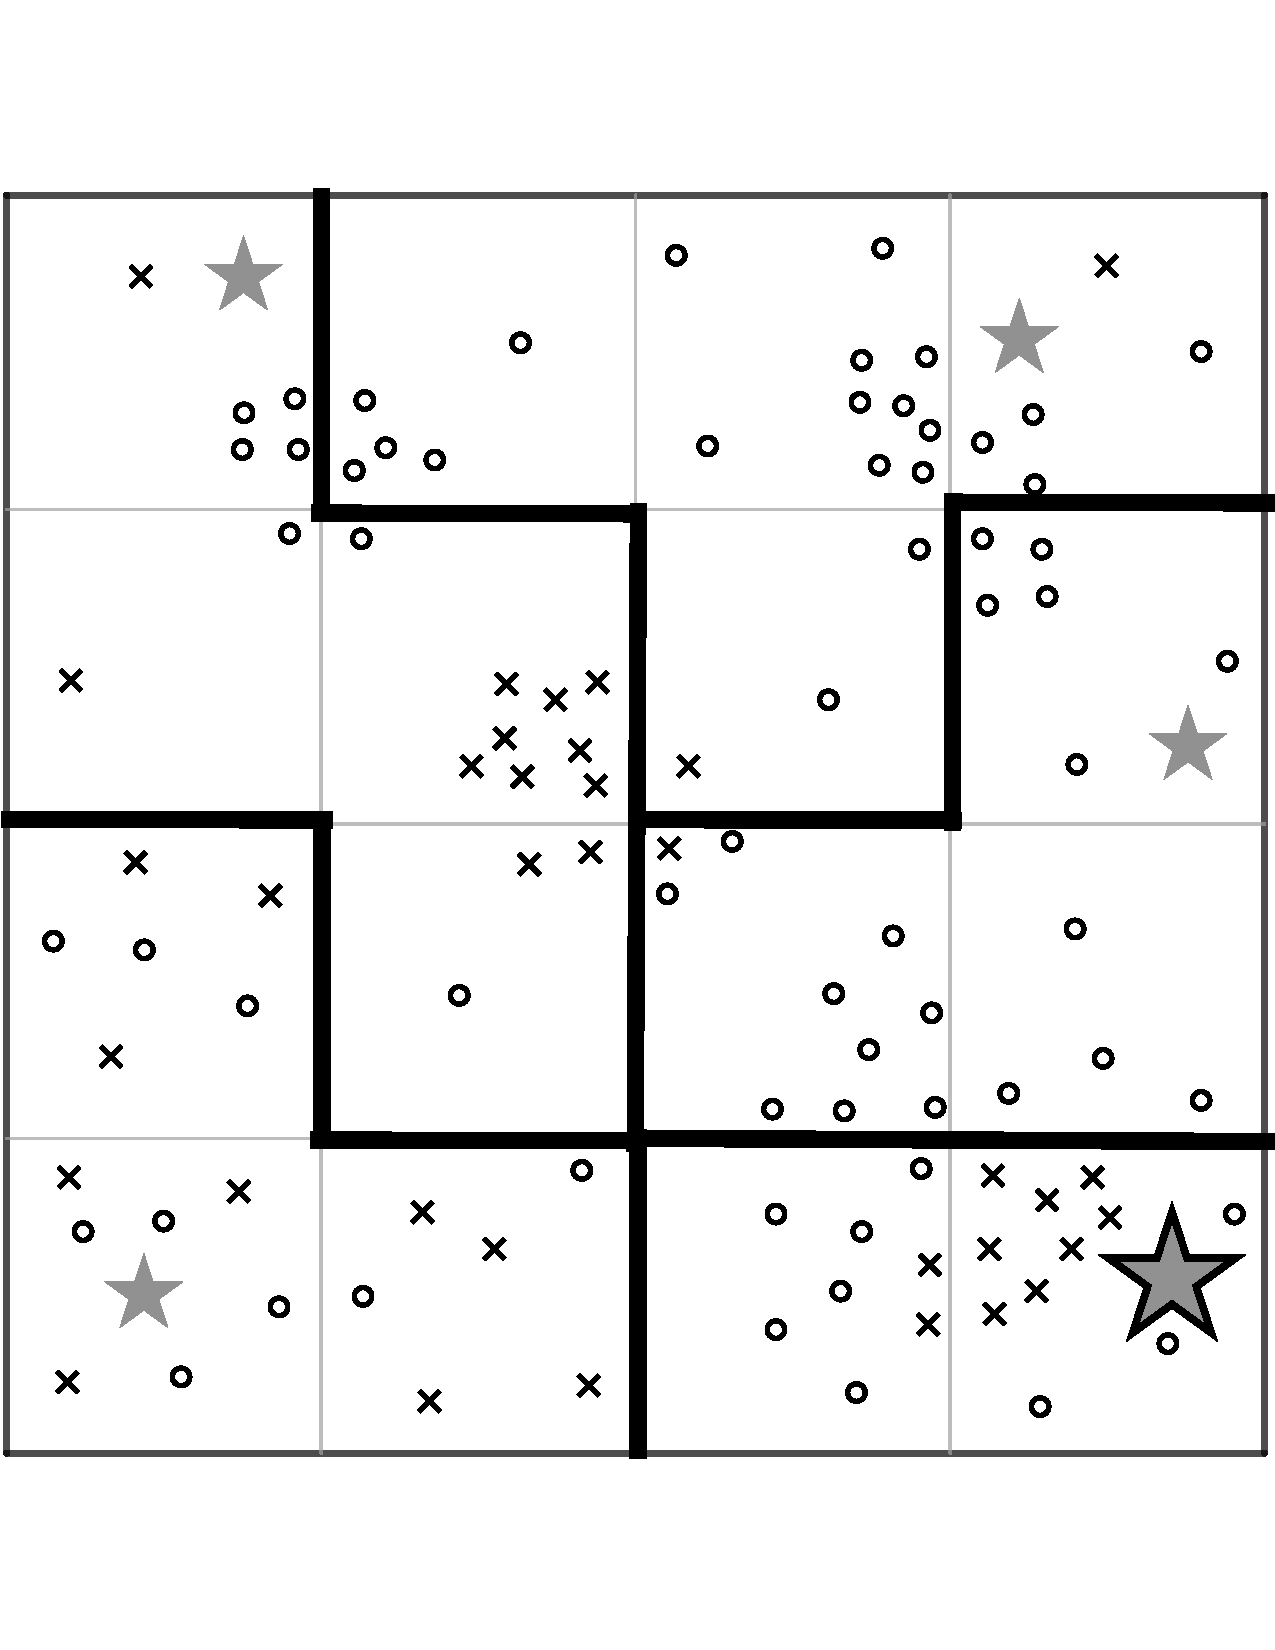
\includegraphics[width=2.5in]{assets/gerrymander-example-solution.pdf}
\hfill\phantom{}


\phChapterWorksheet{Tribe B}{Population = 80}

\begin{center}
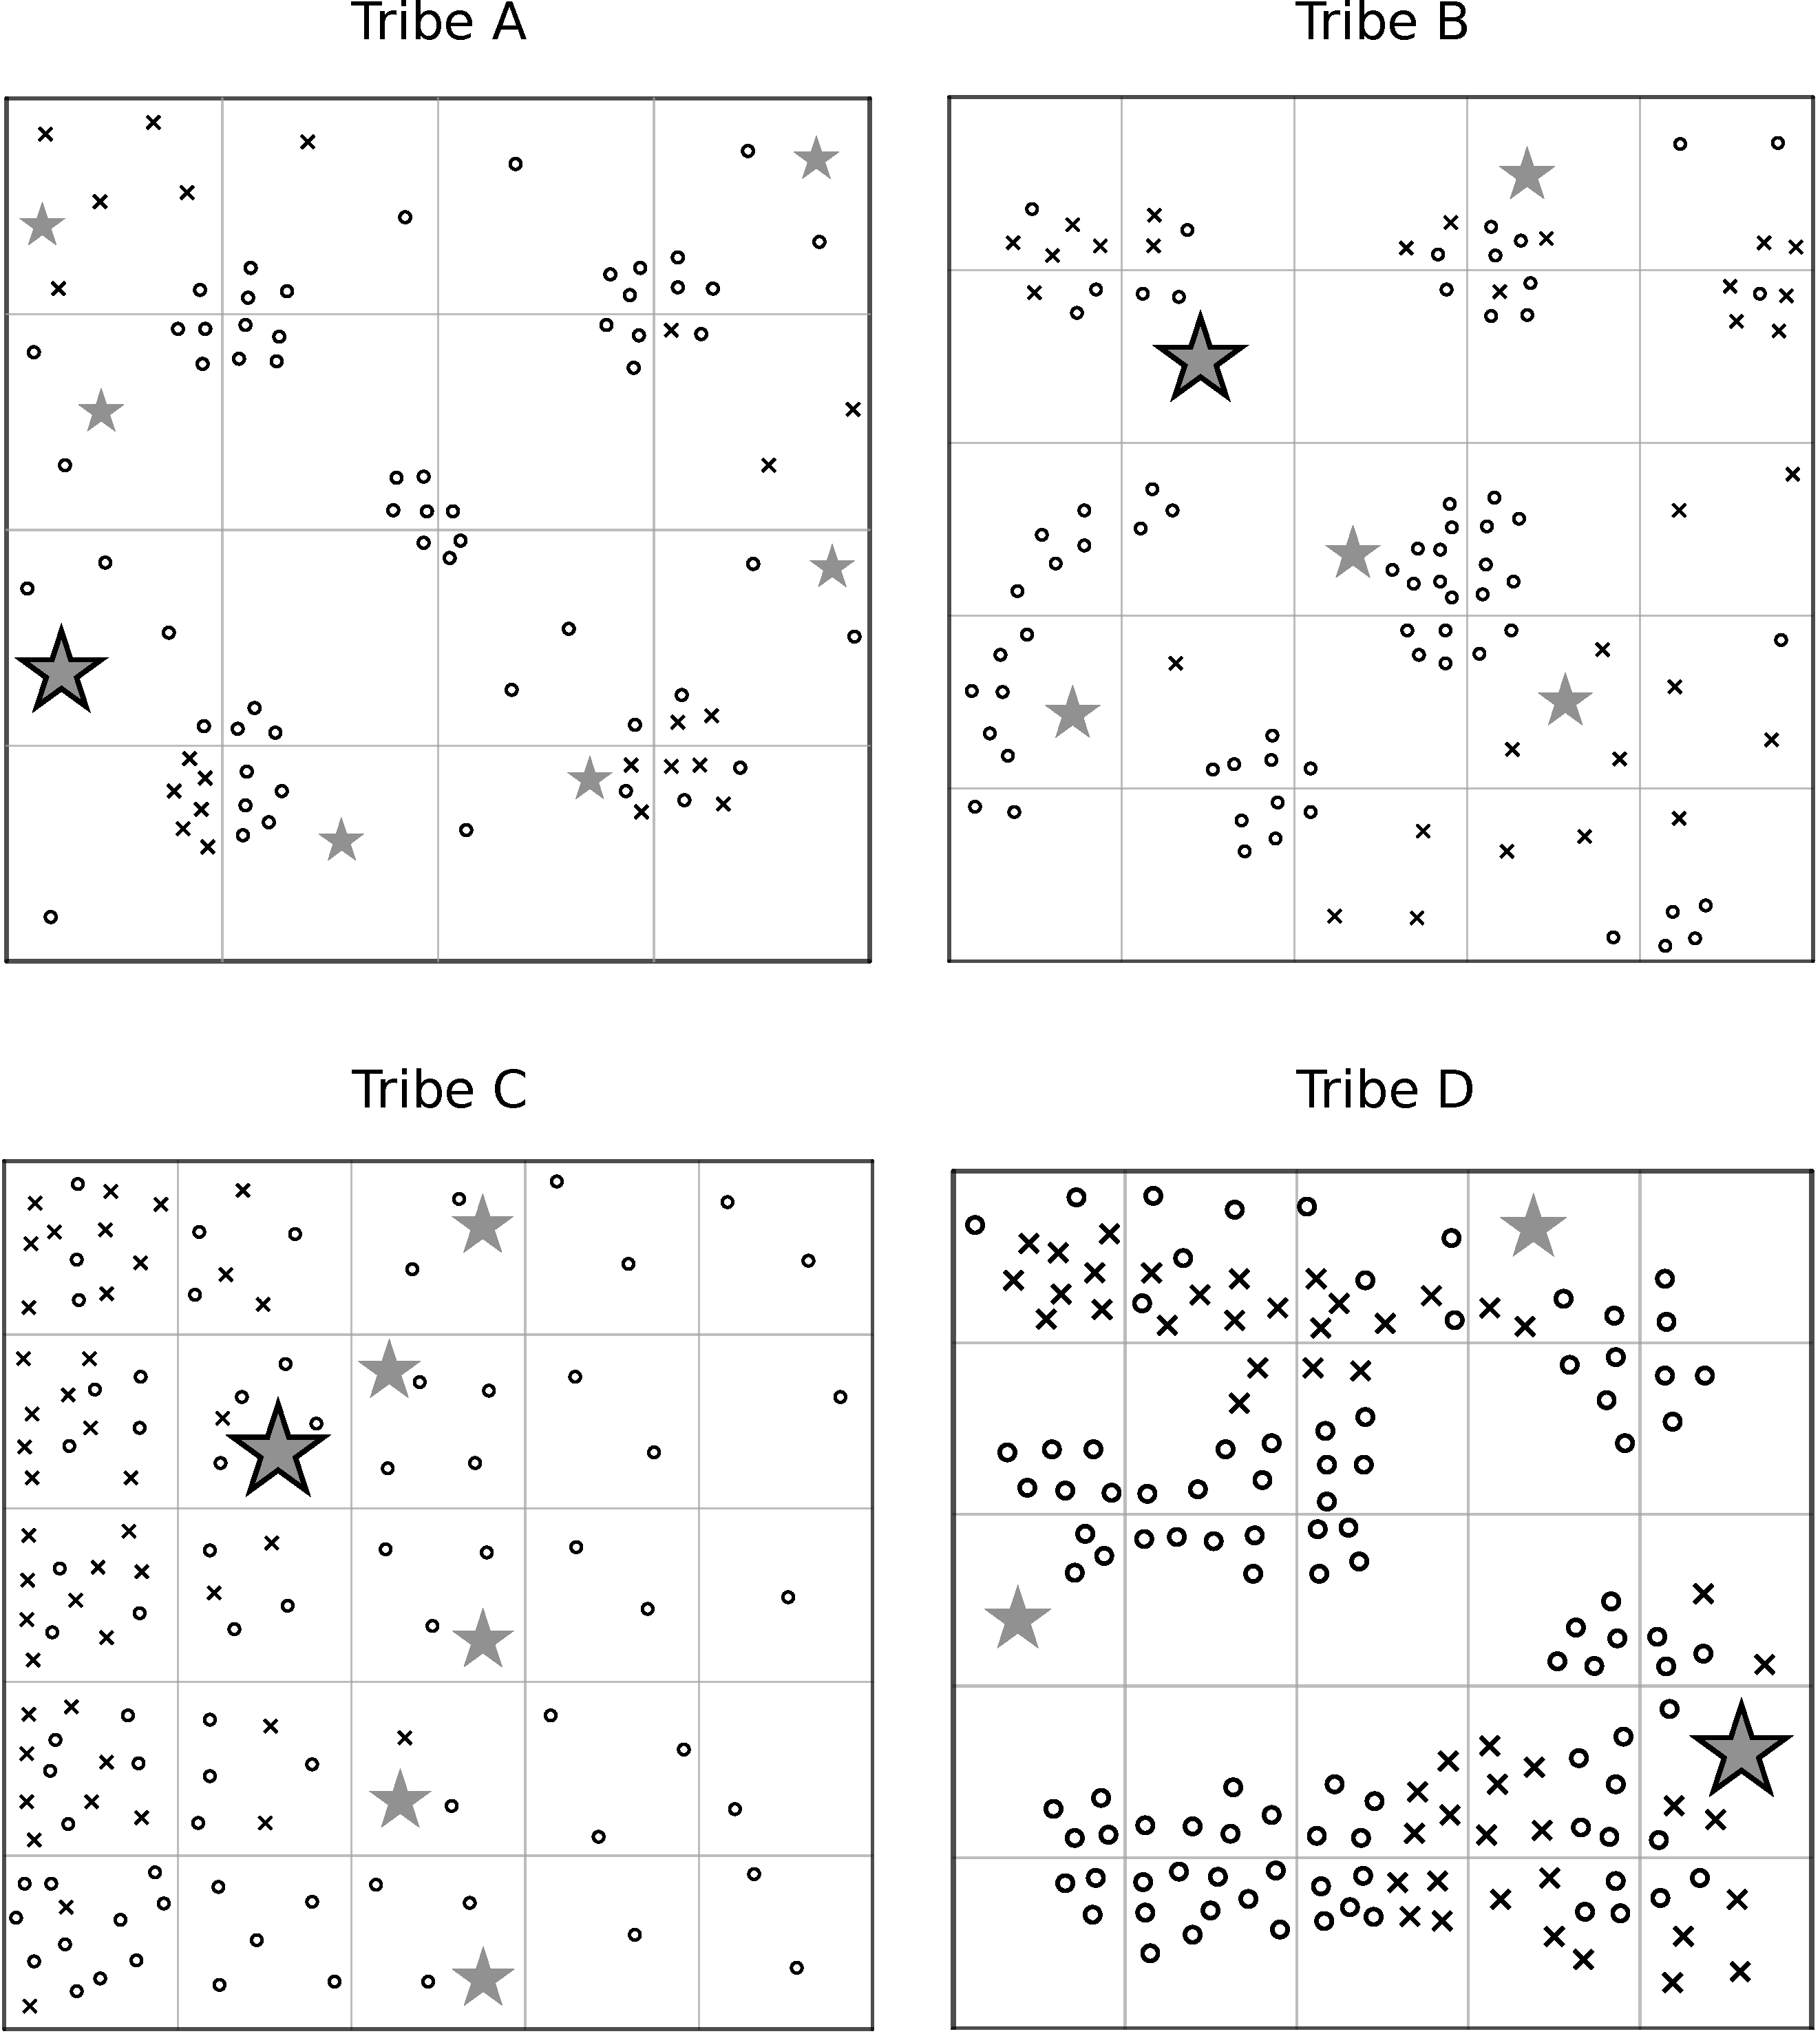
\includegraphics[width=\linewidth]{assets/gerrymanders.pdf}
%\hfill Tribe A \hfill Tribe B \hfill\phantom{}
%
%foo
%
%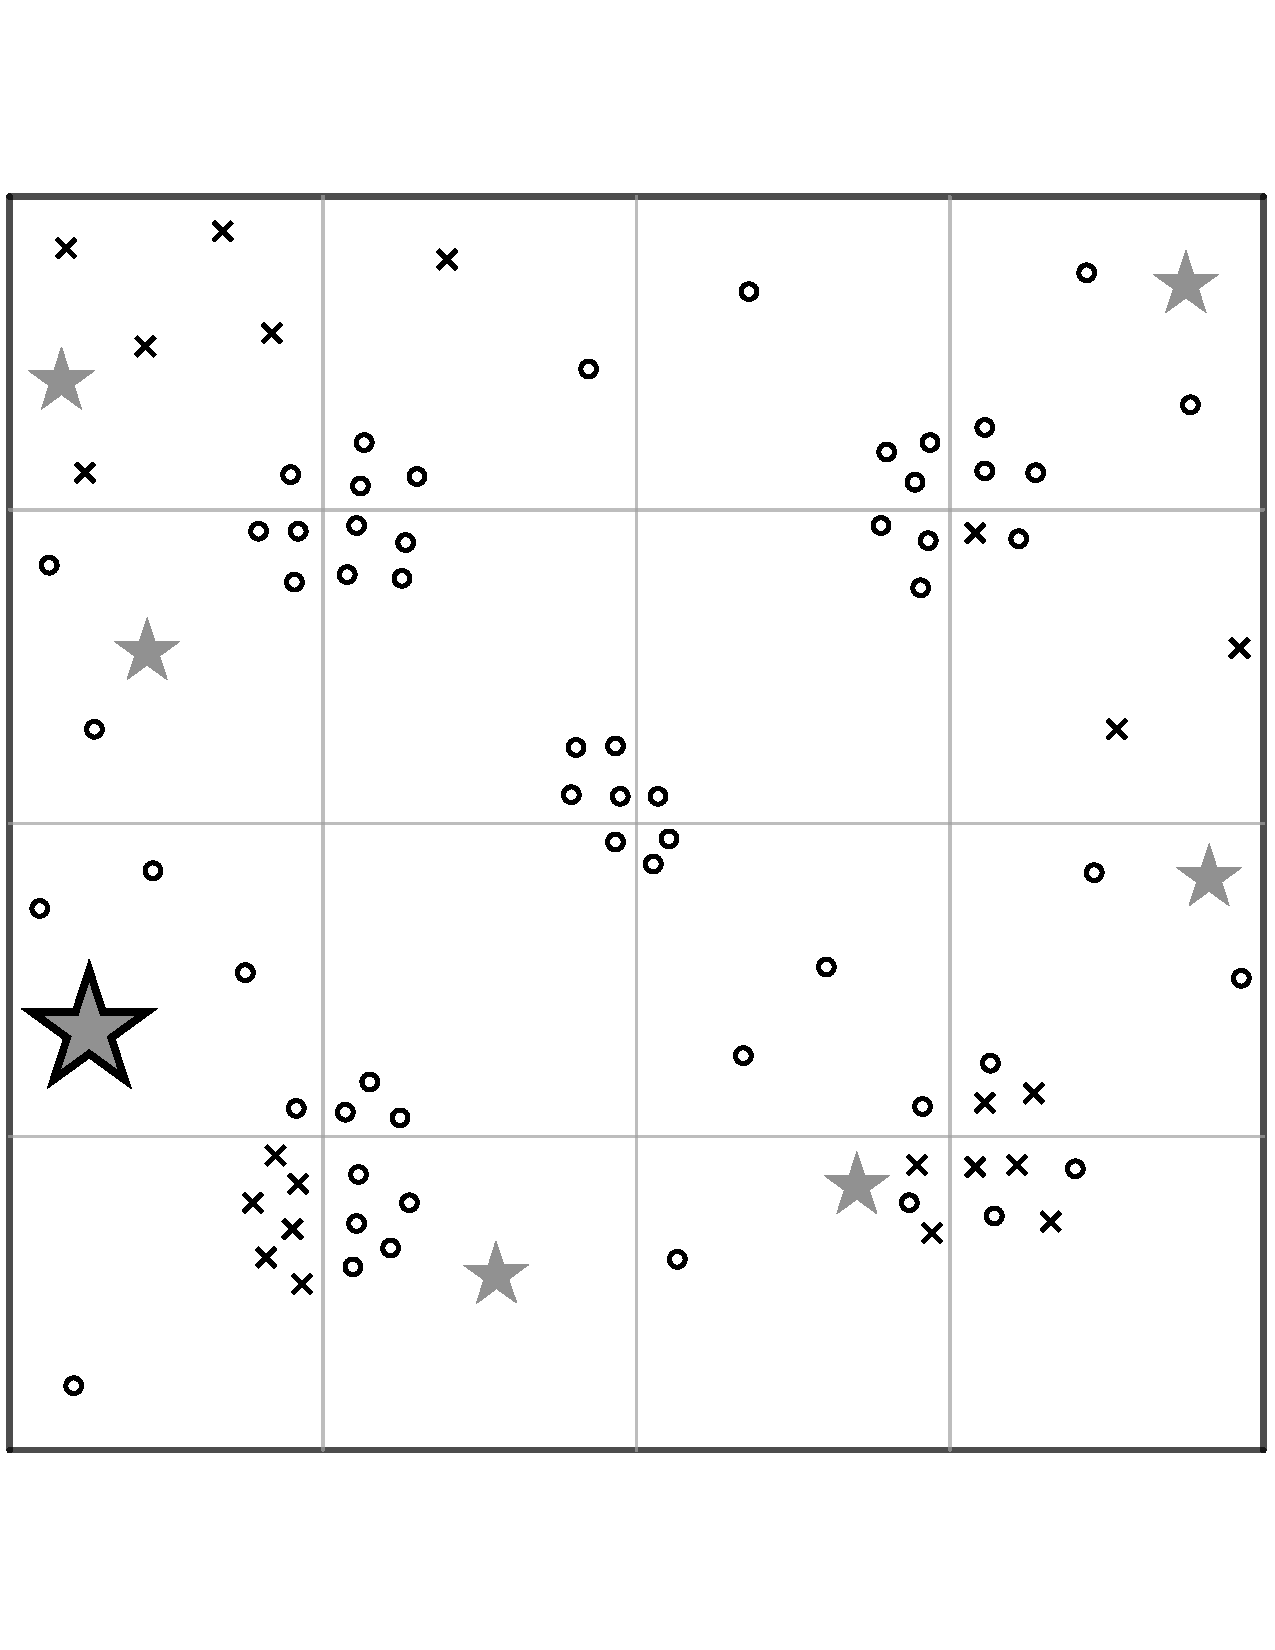
\includegraphics[width=2.8in]{assets/gerrymander-1.pdf}
%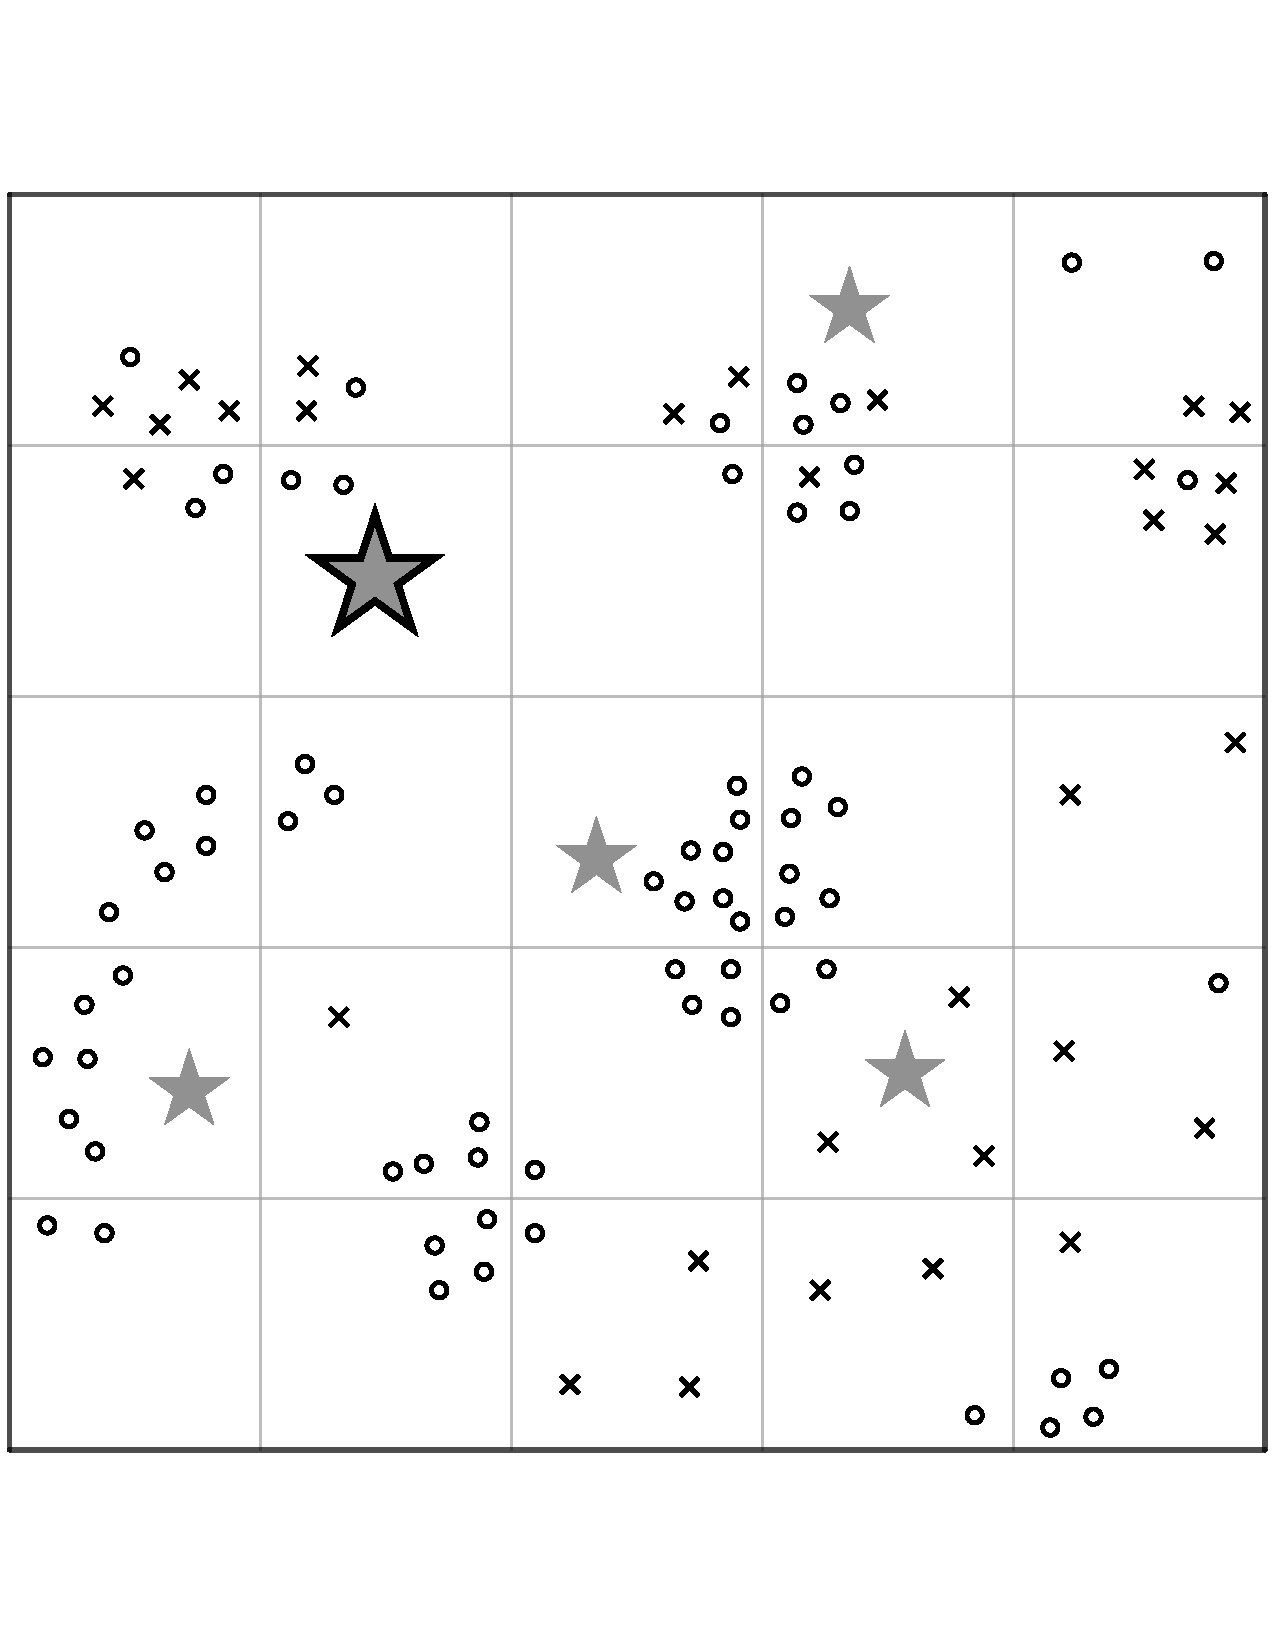
\includegraphics[width=2.8in]{assets/gerrymander-2.pdf}
%
%\hfill Tribe C \hfill Tribe D \hfill\phantom{}
%
%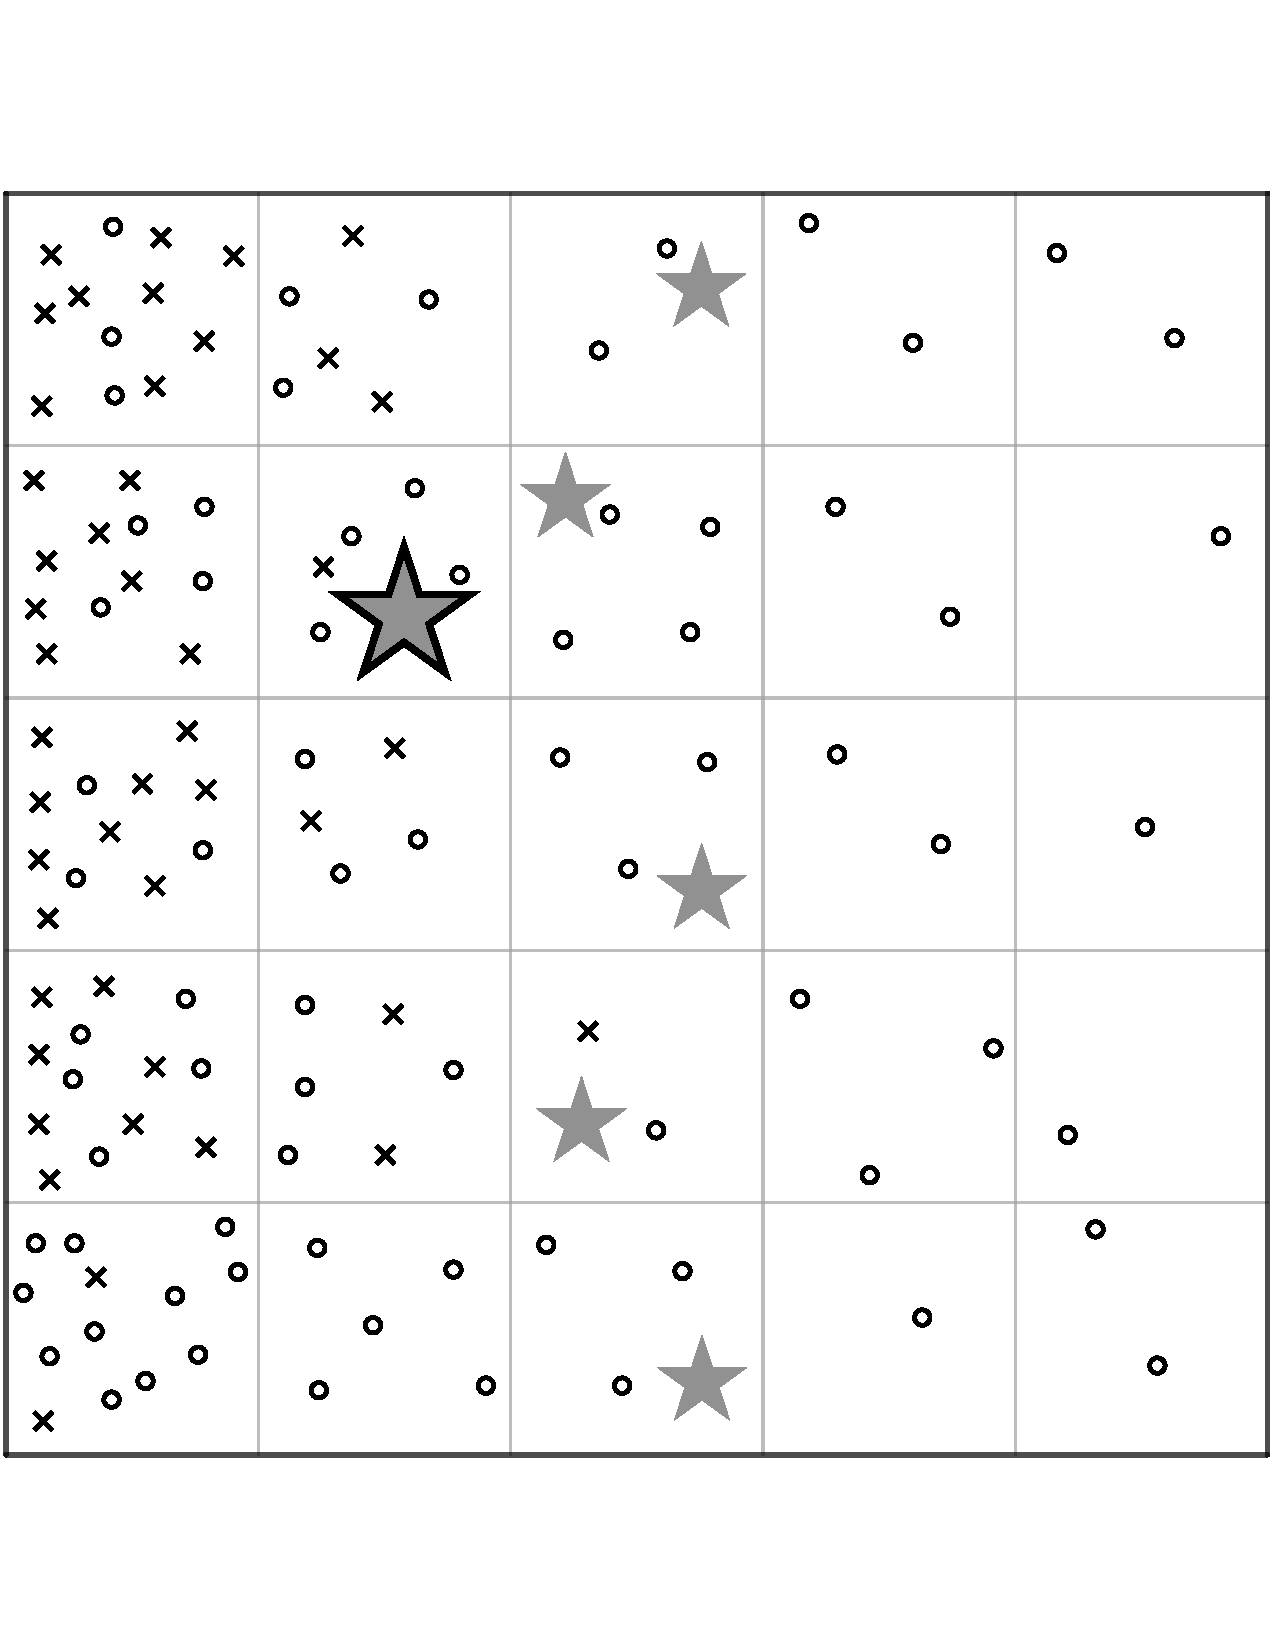
\includegraphics[width=2.8in]{assets/gerrymander-3.pdf}
%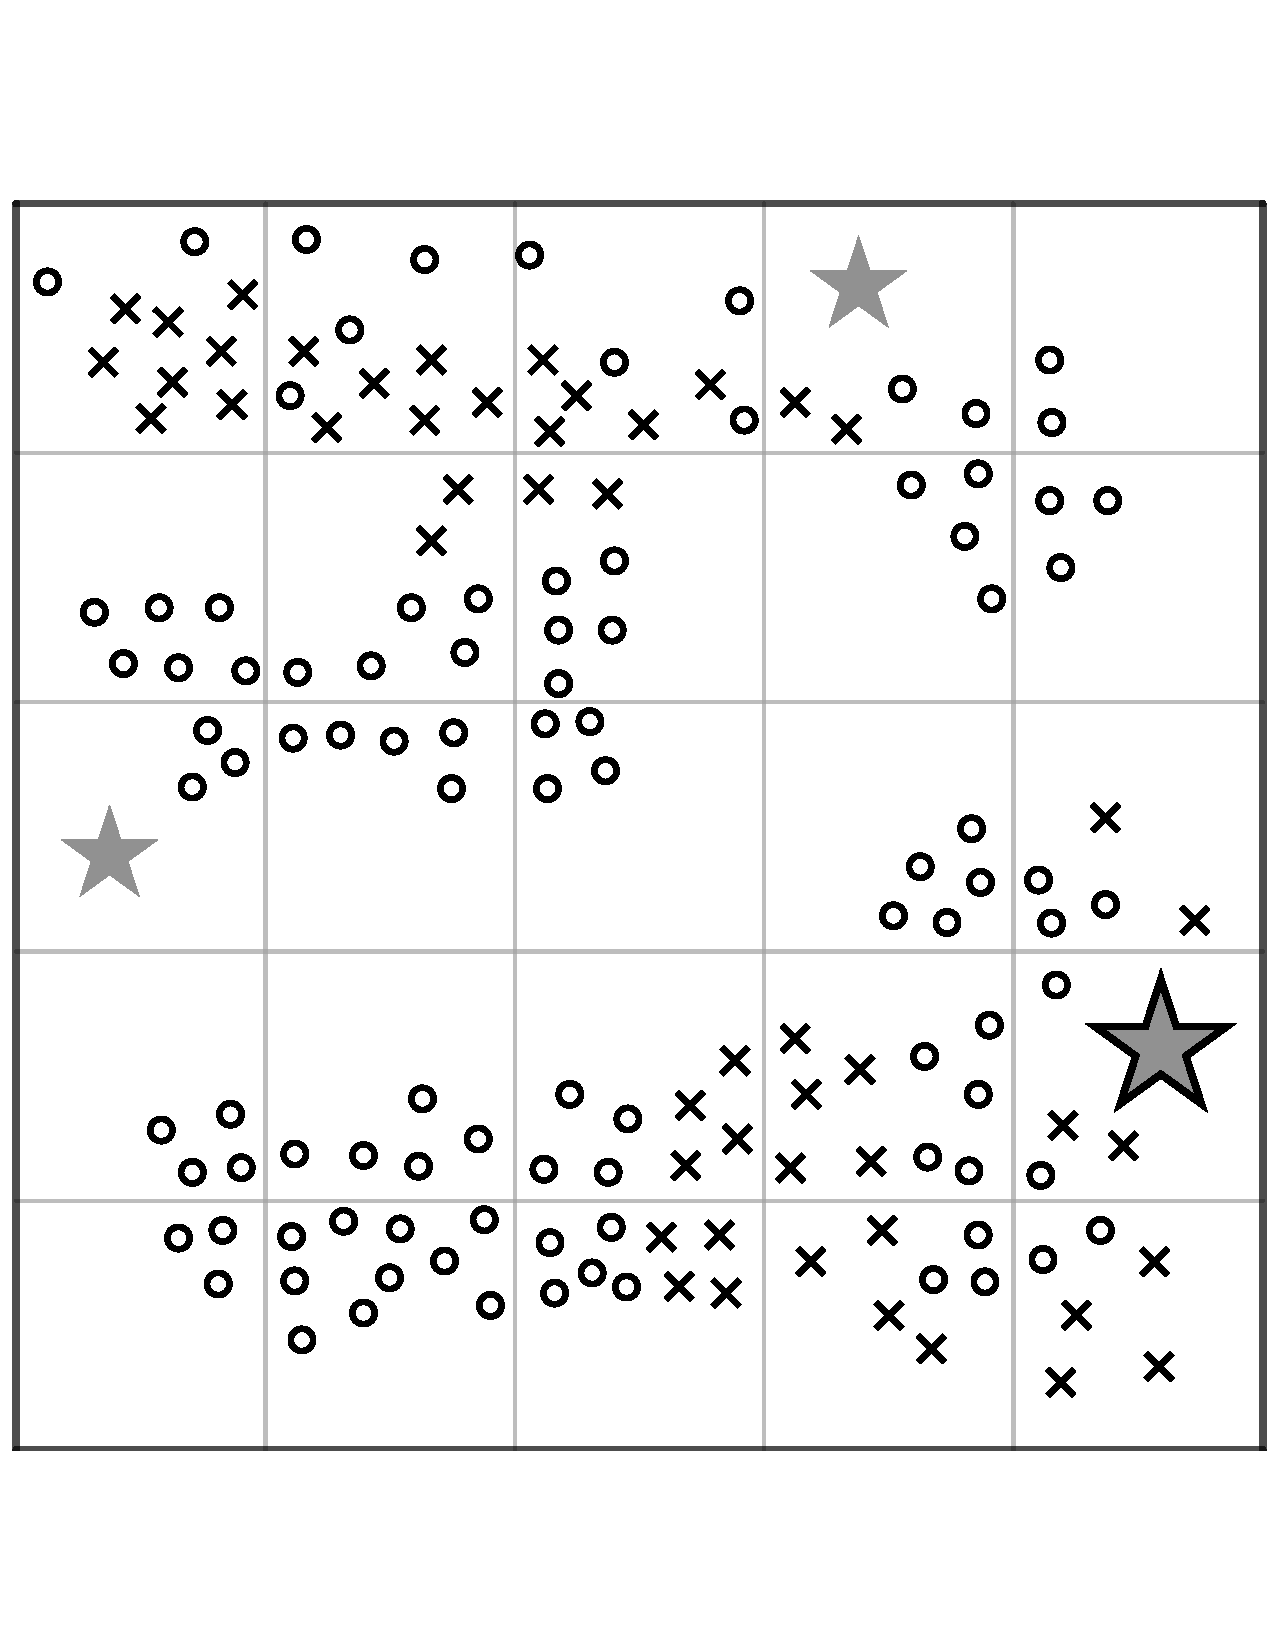
\includegraphics[width=2.8in]{assets/gerrymander-4.pdf}
\end{center}

%\begin{tabular}{c c c }
%
%Year 1 & Year 2 & Year 3 \\
% 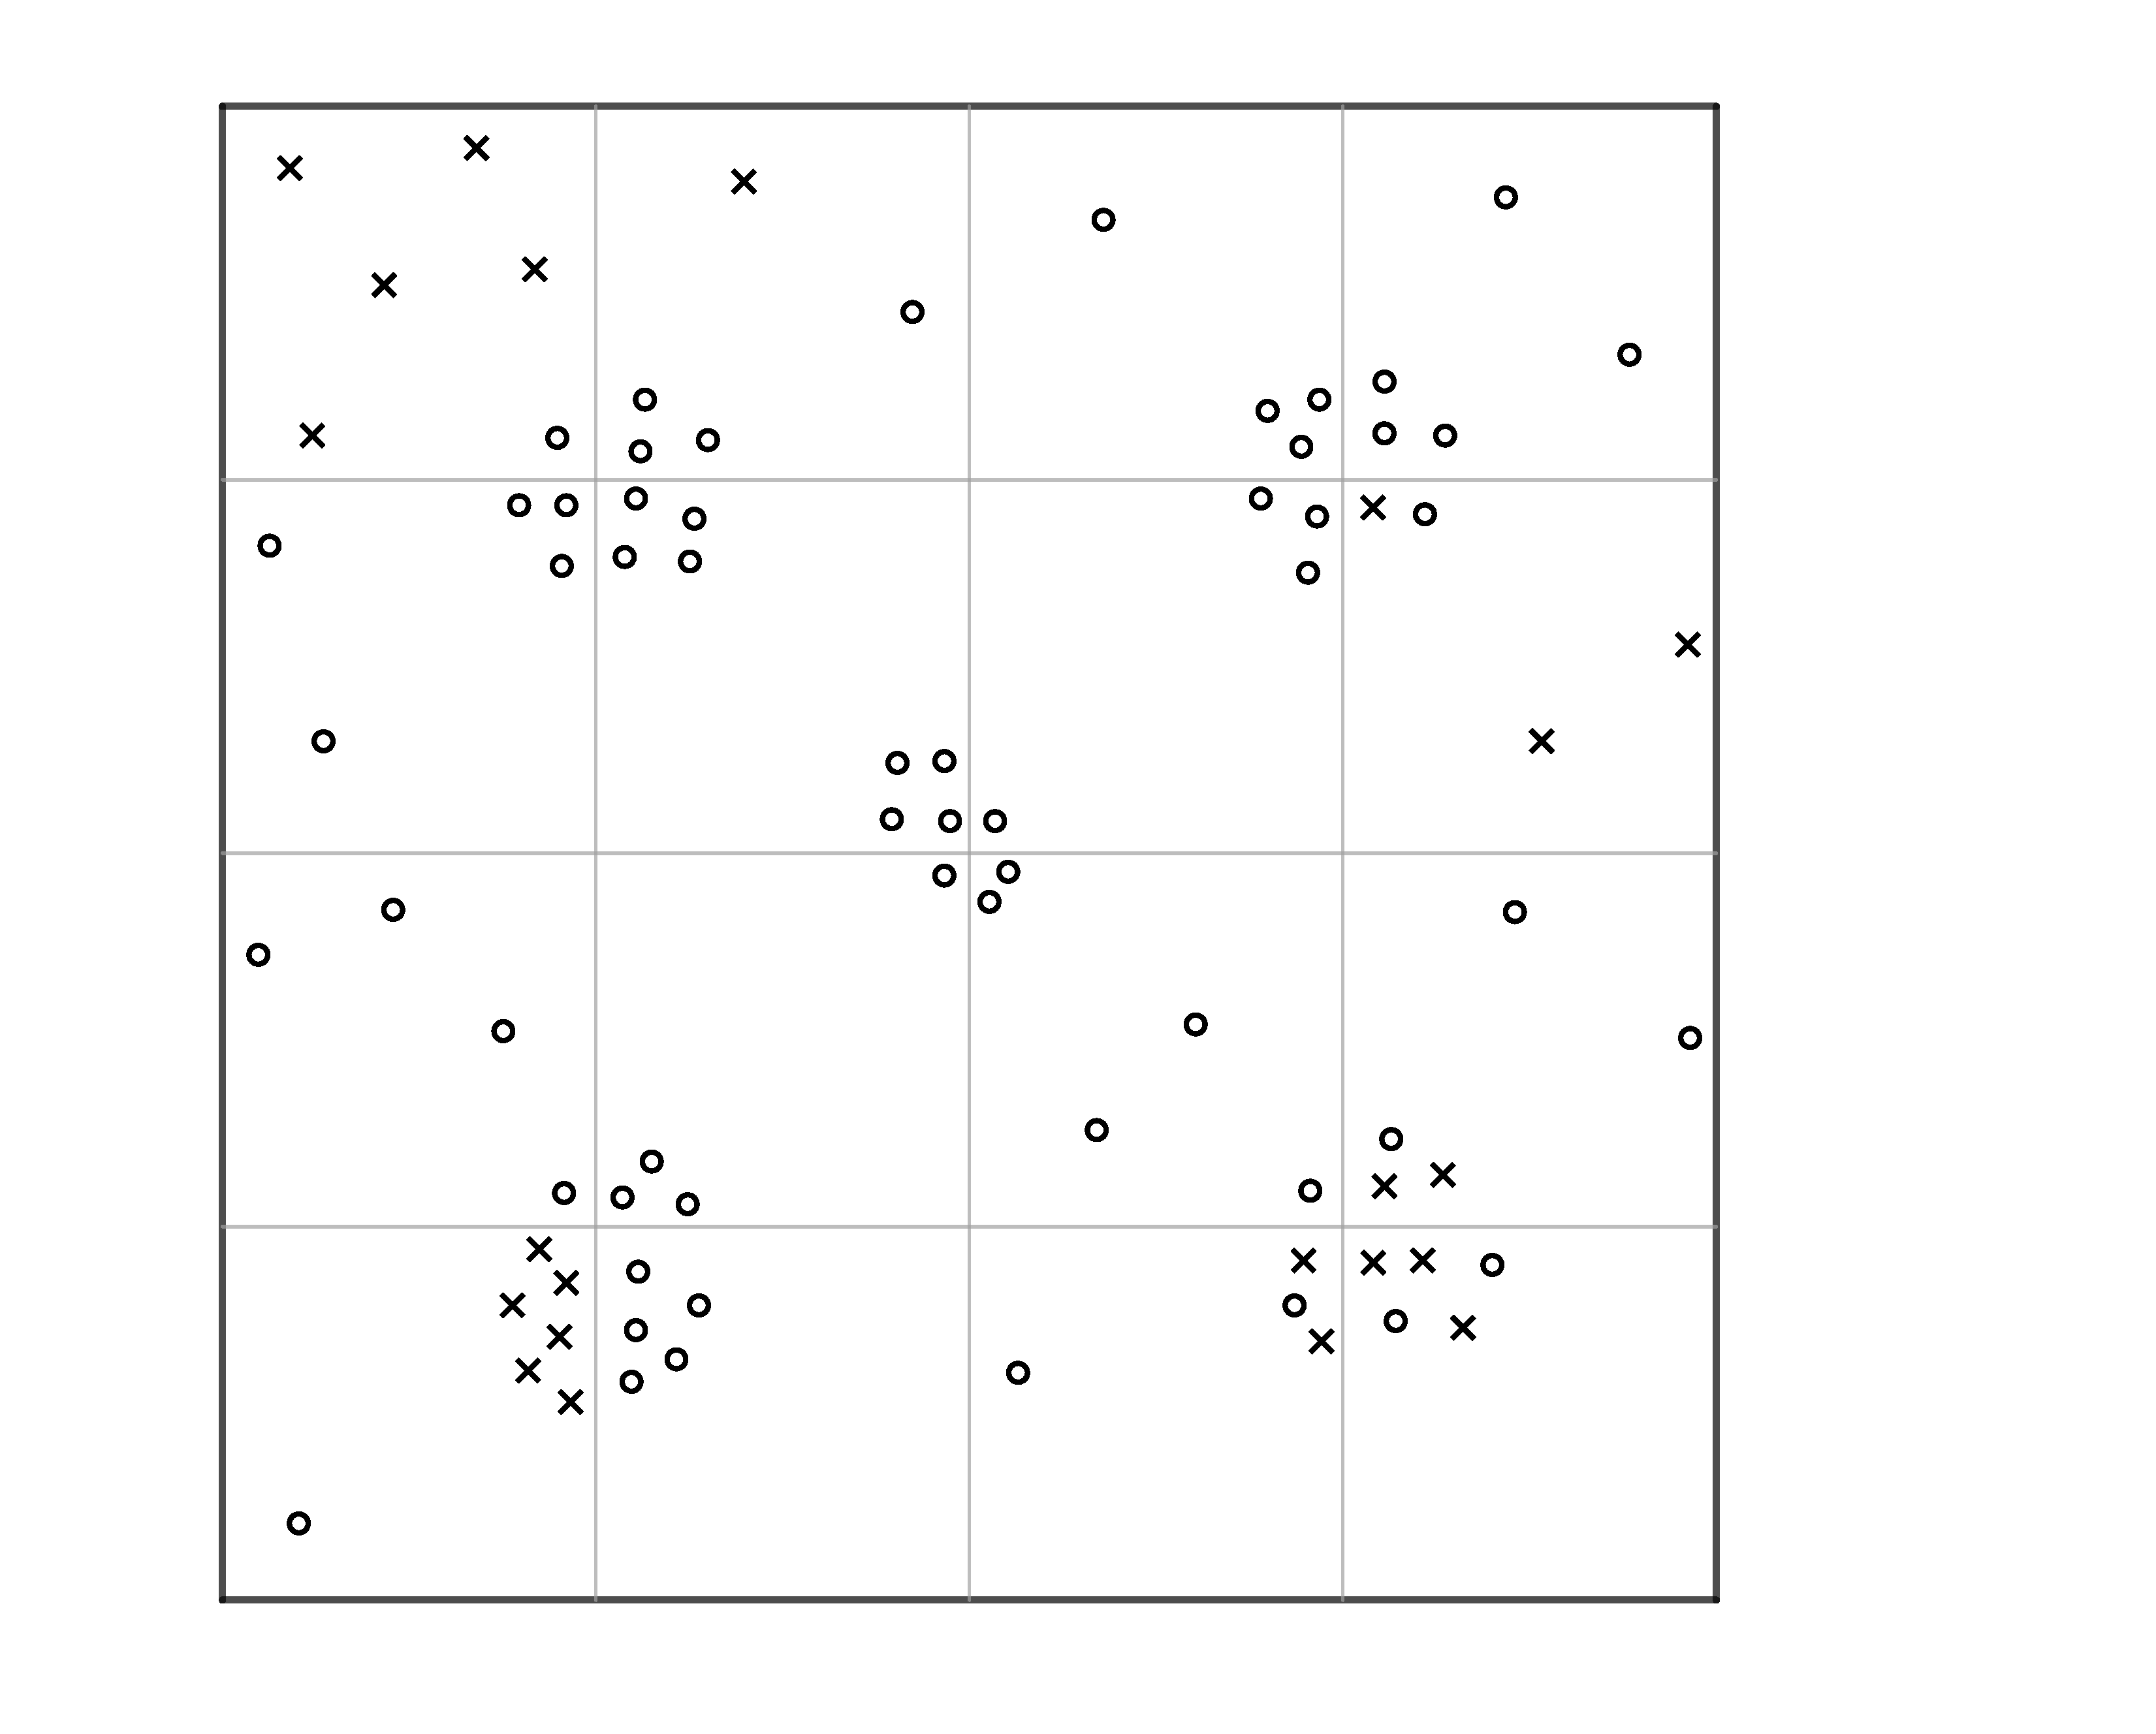
\includegraphics[width=1in]{assets/Gerrymandering/Gerry4x4-80-1.pdf} &  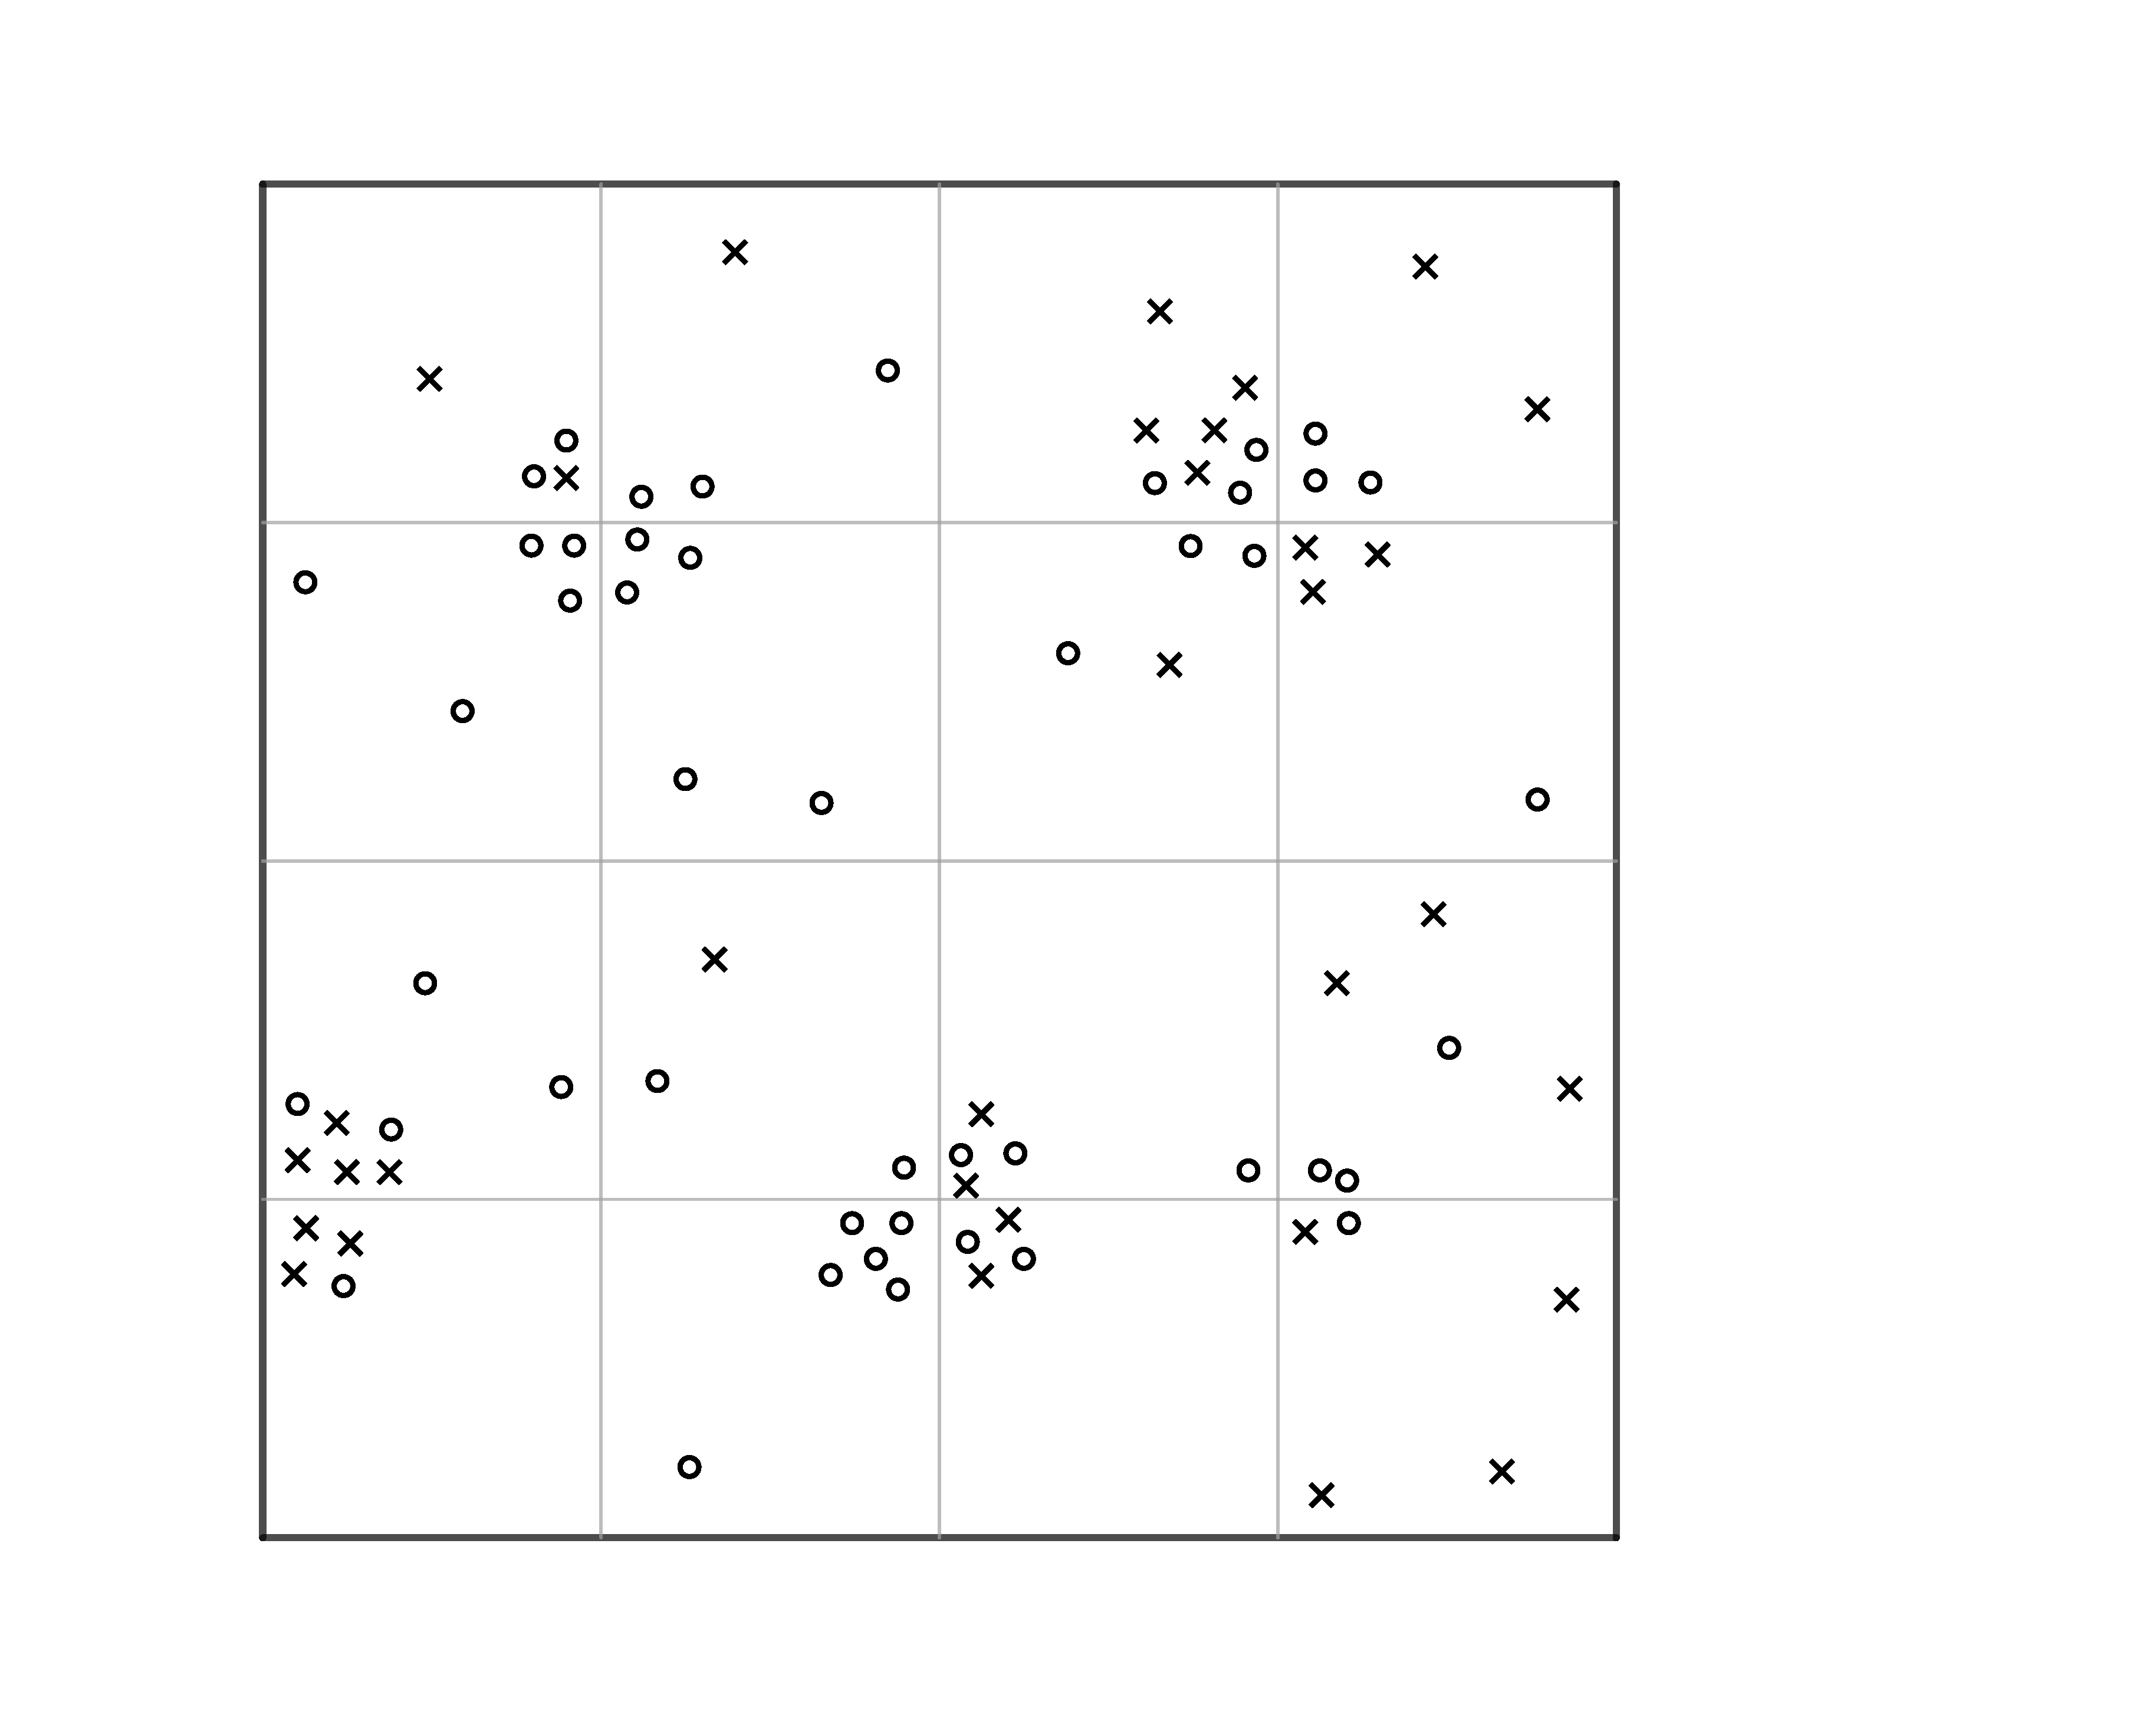
\includegraphics[width=1in]{assets/Gerrymandering/Gerry4x4-80-2.pdf} &  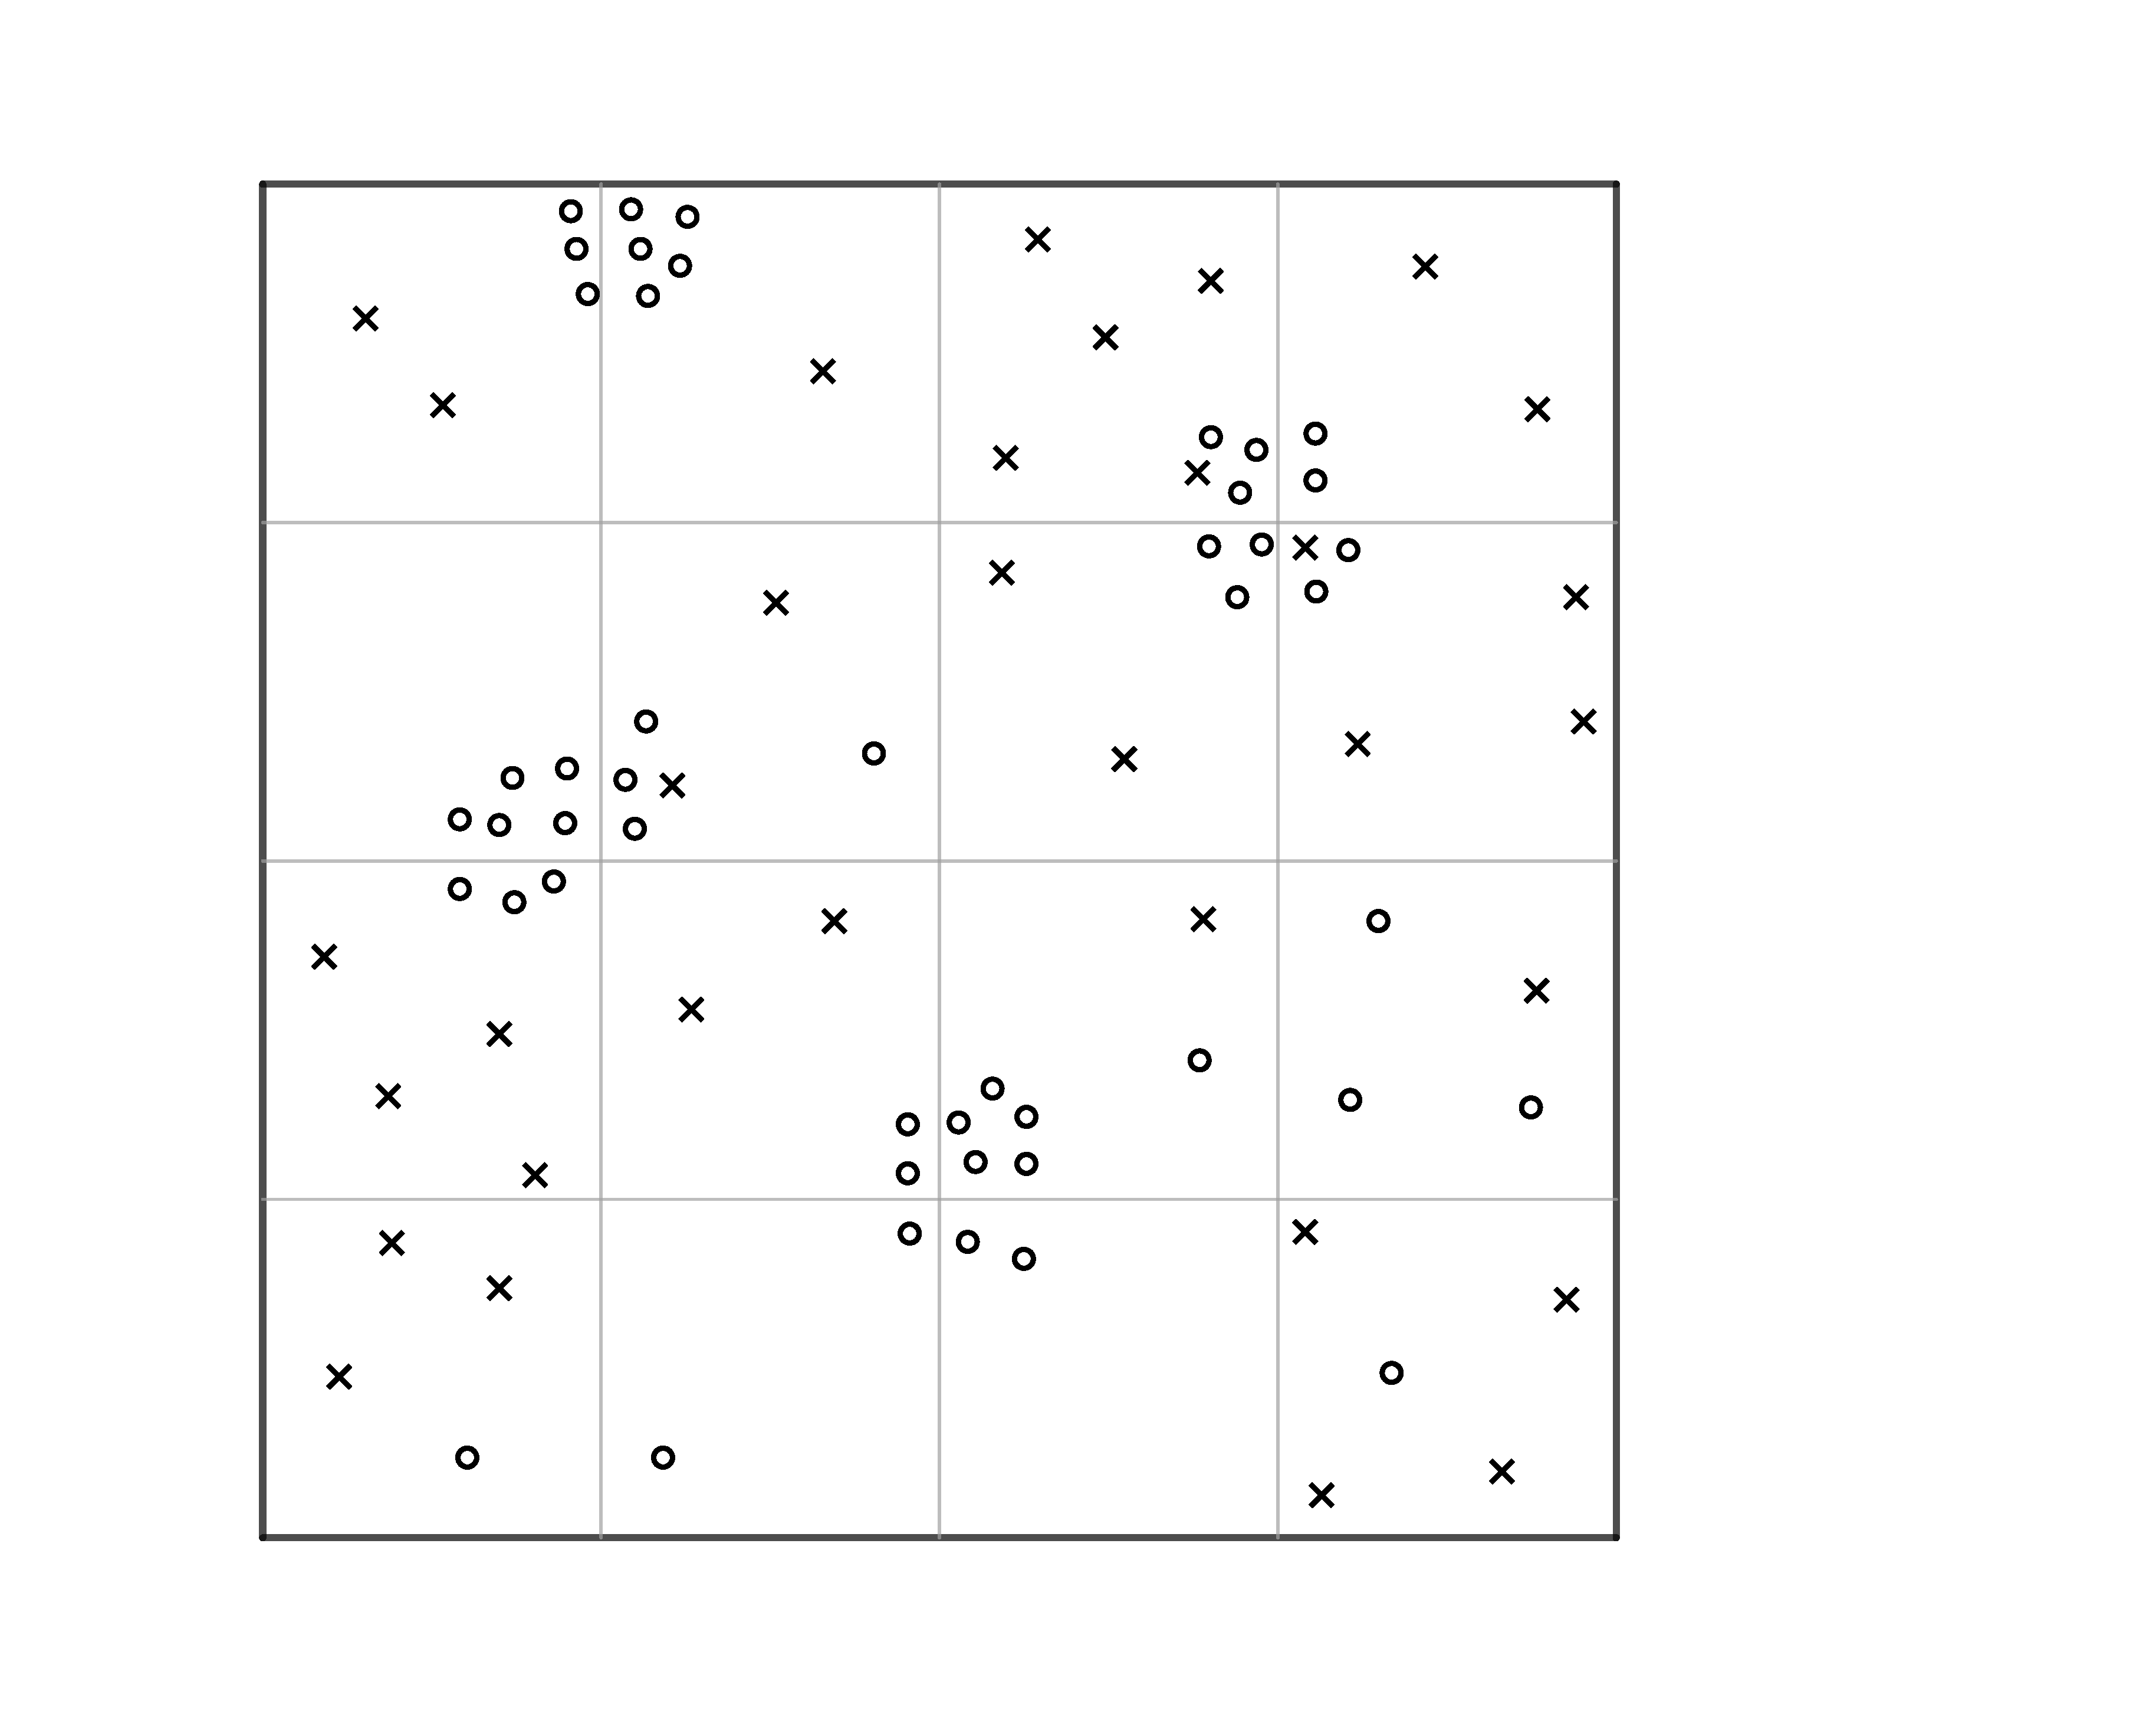
\includegraphics[width=1in]{assets/Gerrymandering/Gerry4x4-80-3.pdf}\\
% Total Vote Count &  Total Vote Count &  Total Vote Count\\
% X -  22& X - 33 & X  - 33\\
% O - 58 & O - 47 & O - 47
% \end{tabular}
%\begin{tabular}{c c c }
%
%Year 1 & Year 2 & Year 3 \\
% 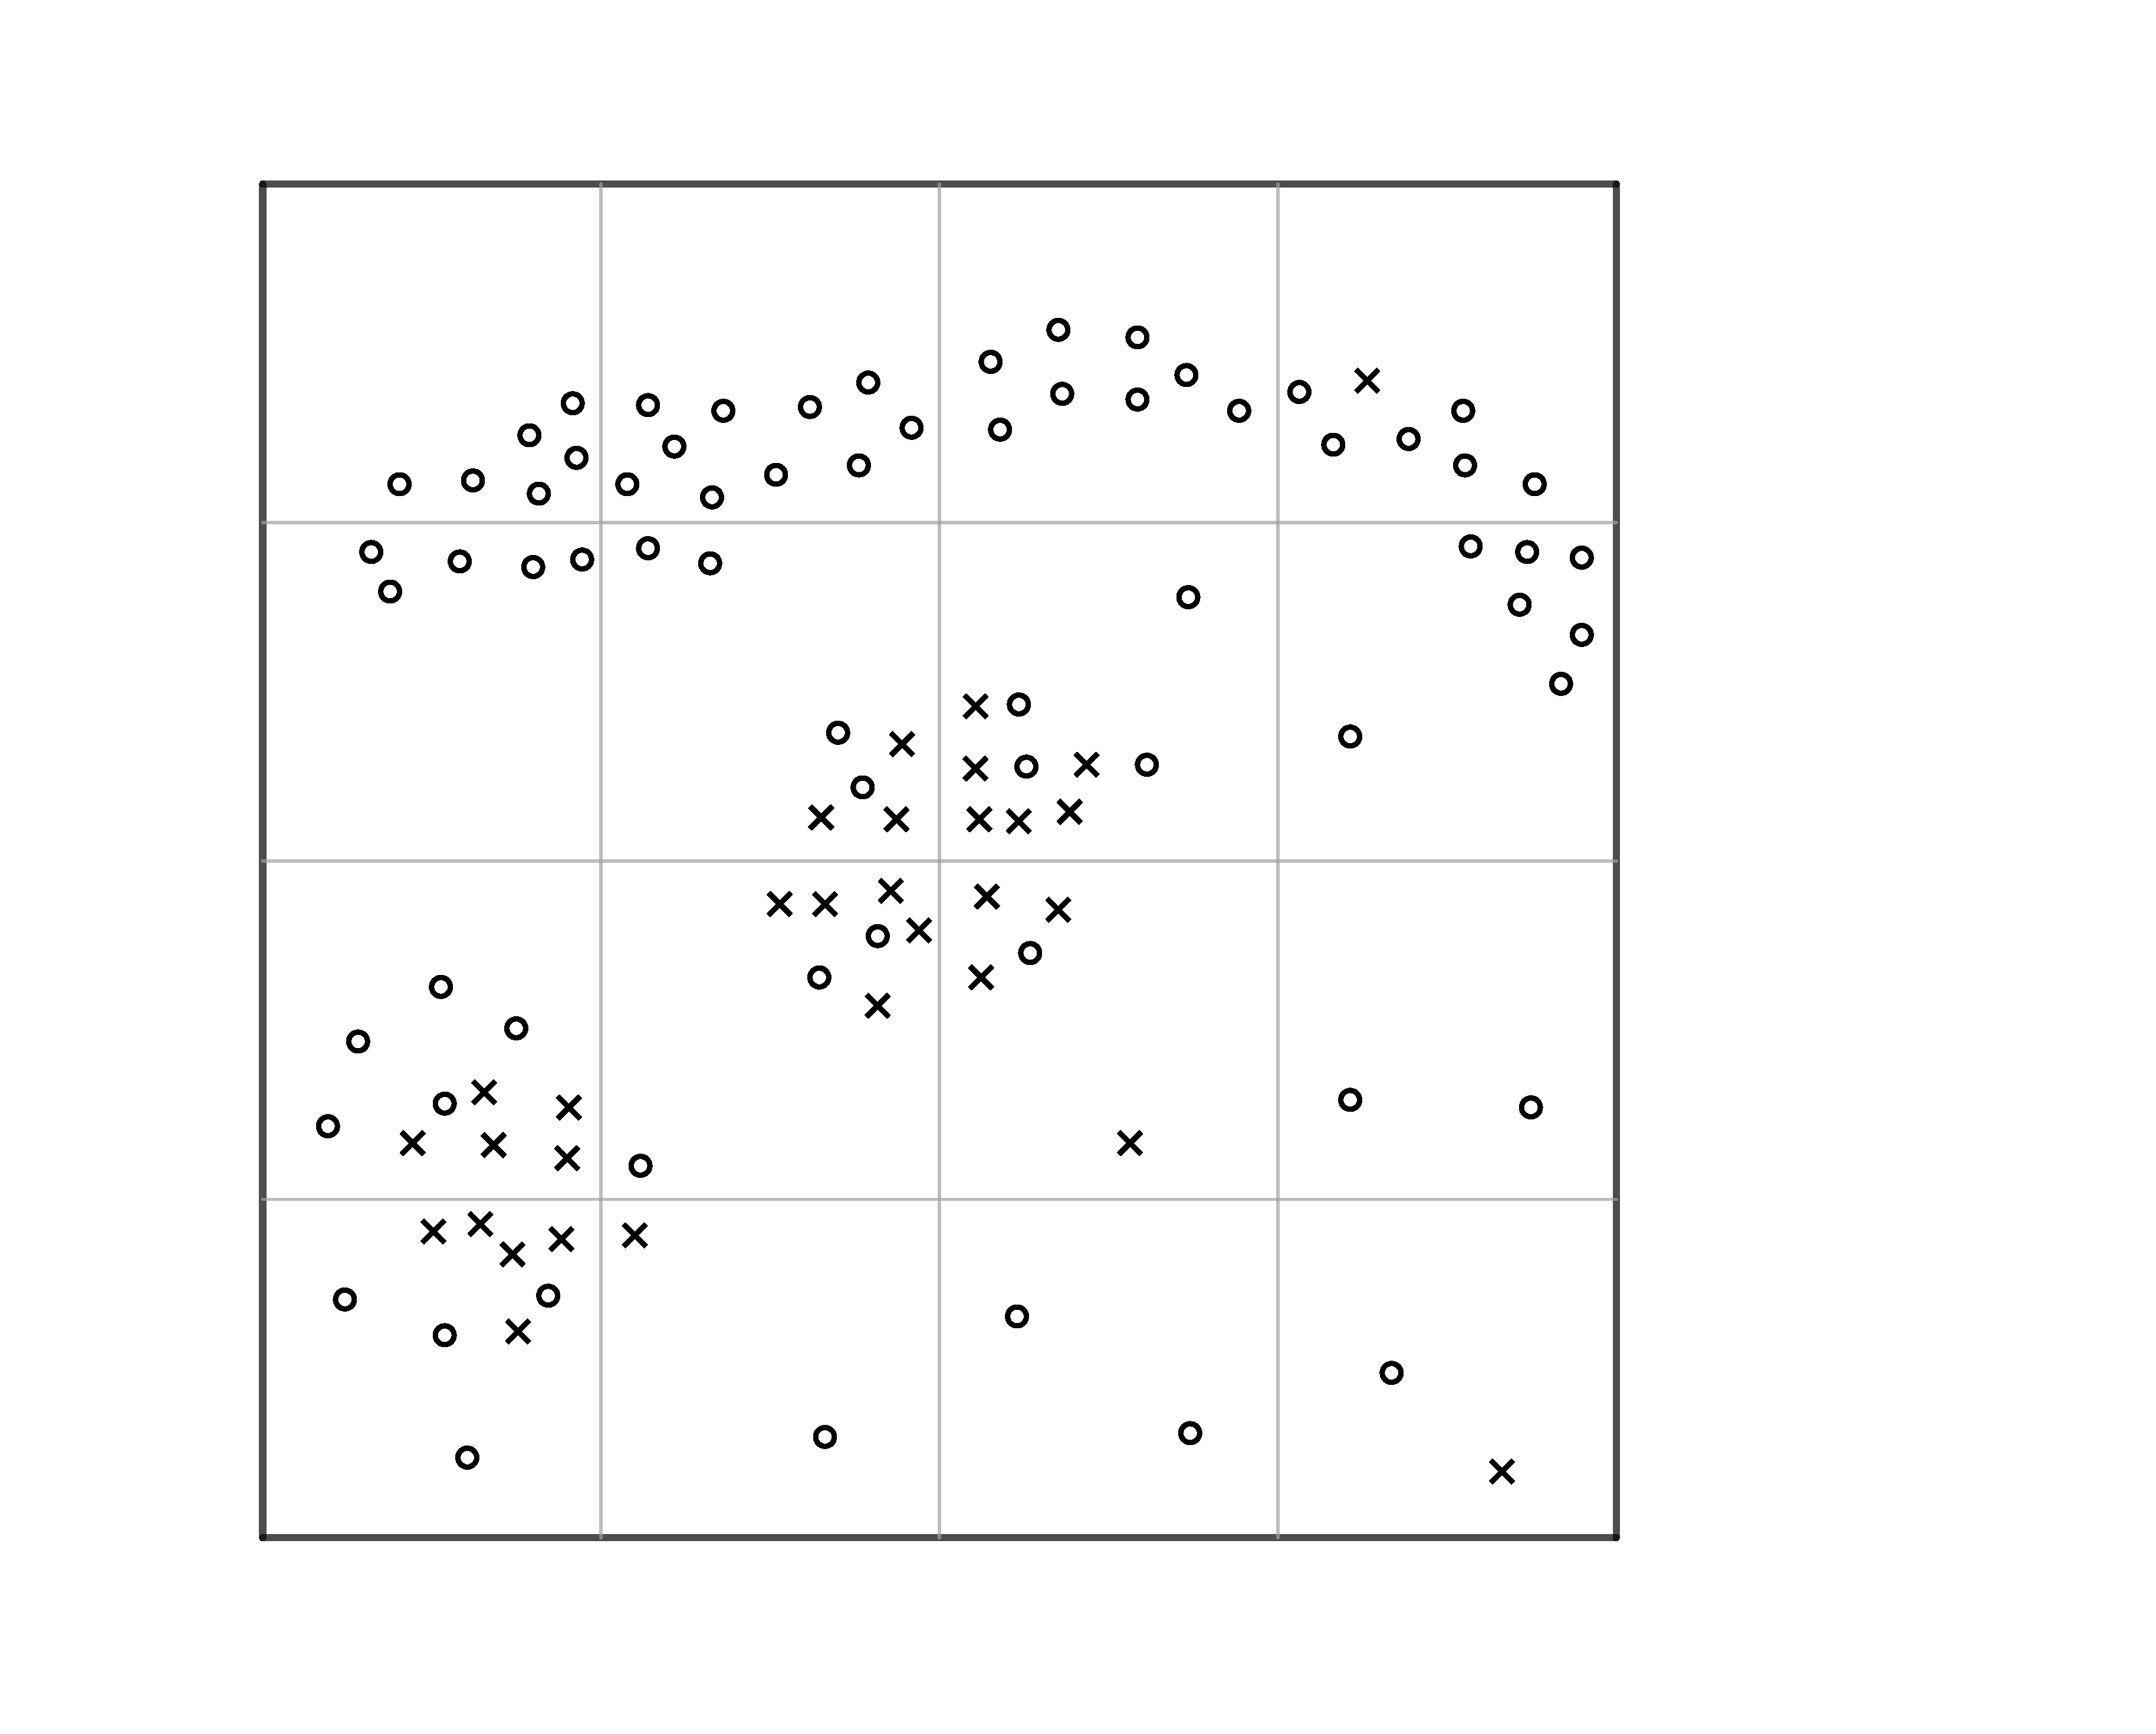
\includegraphics[width=1in]{assets/Gerrymandering/Gerry4x4-100-1.pdf} &  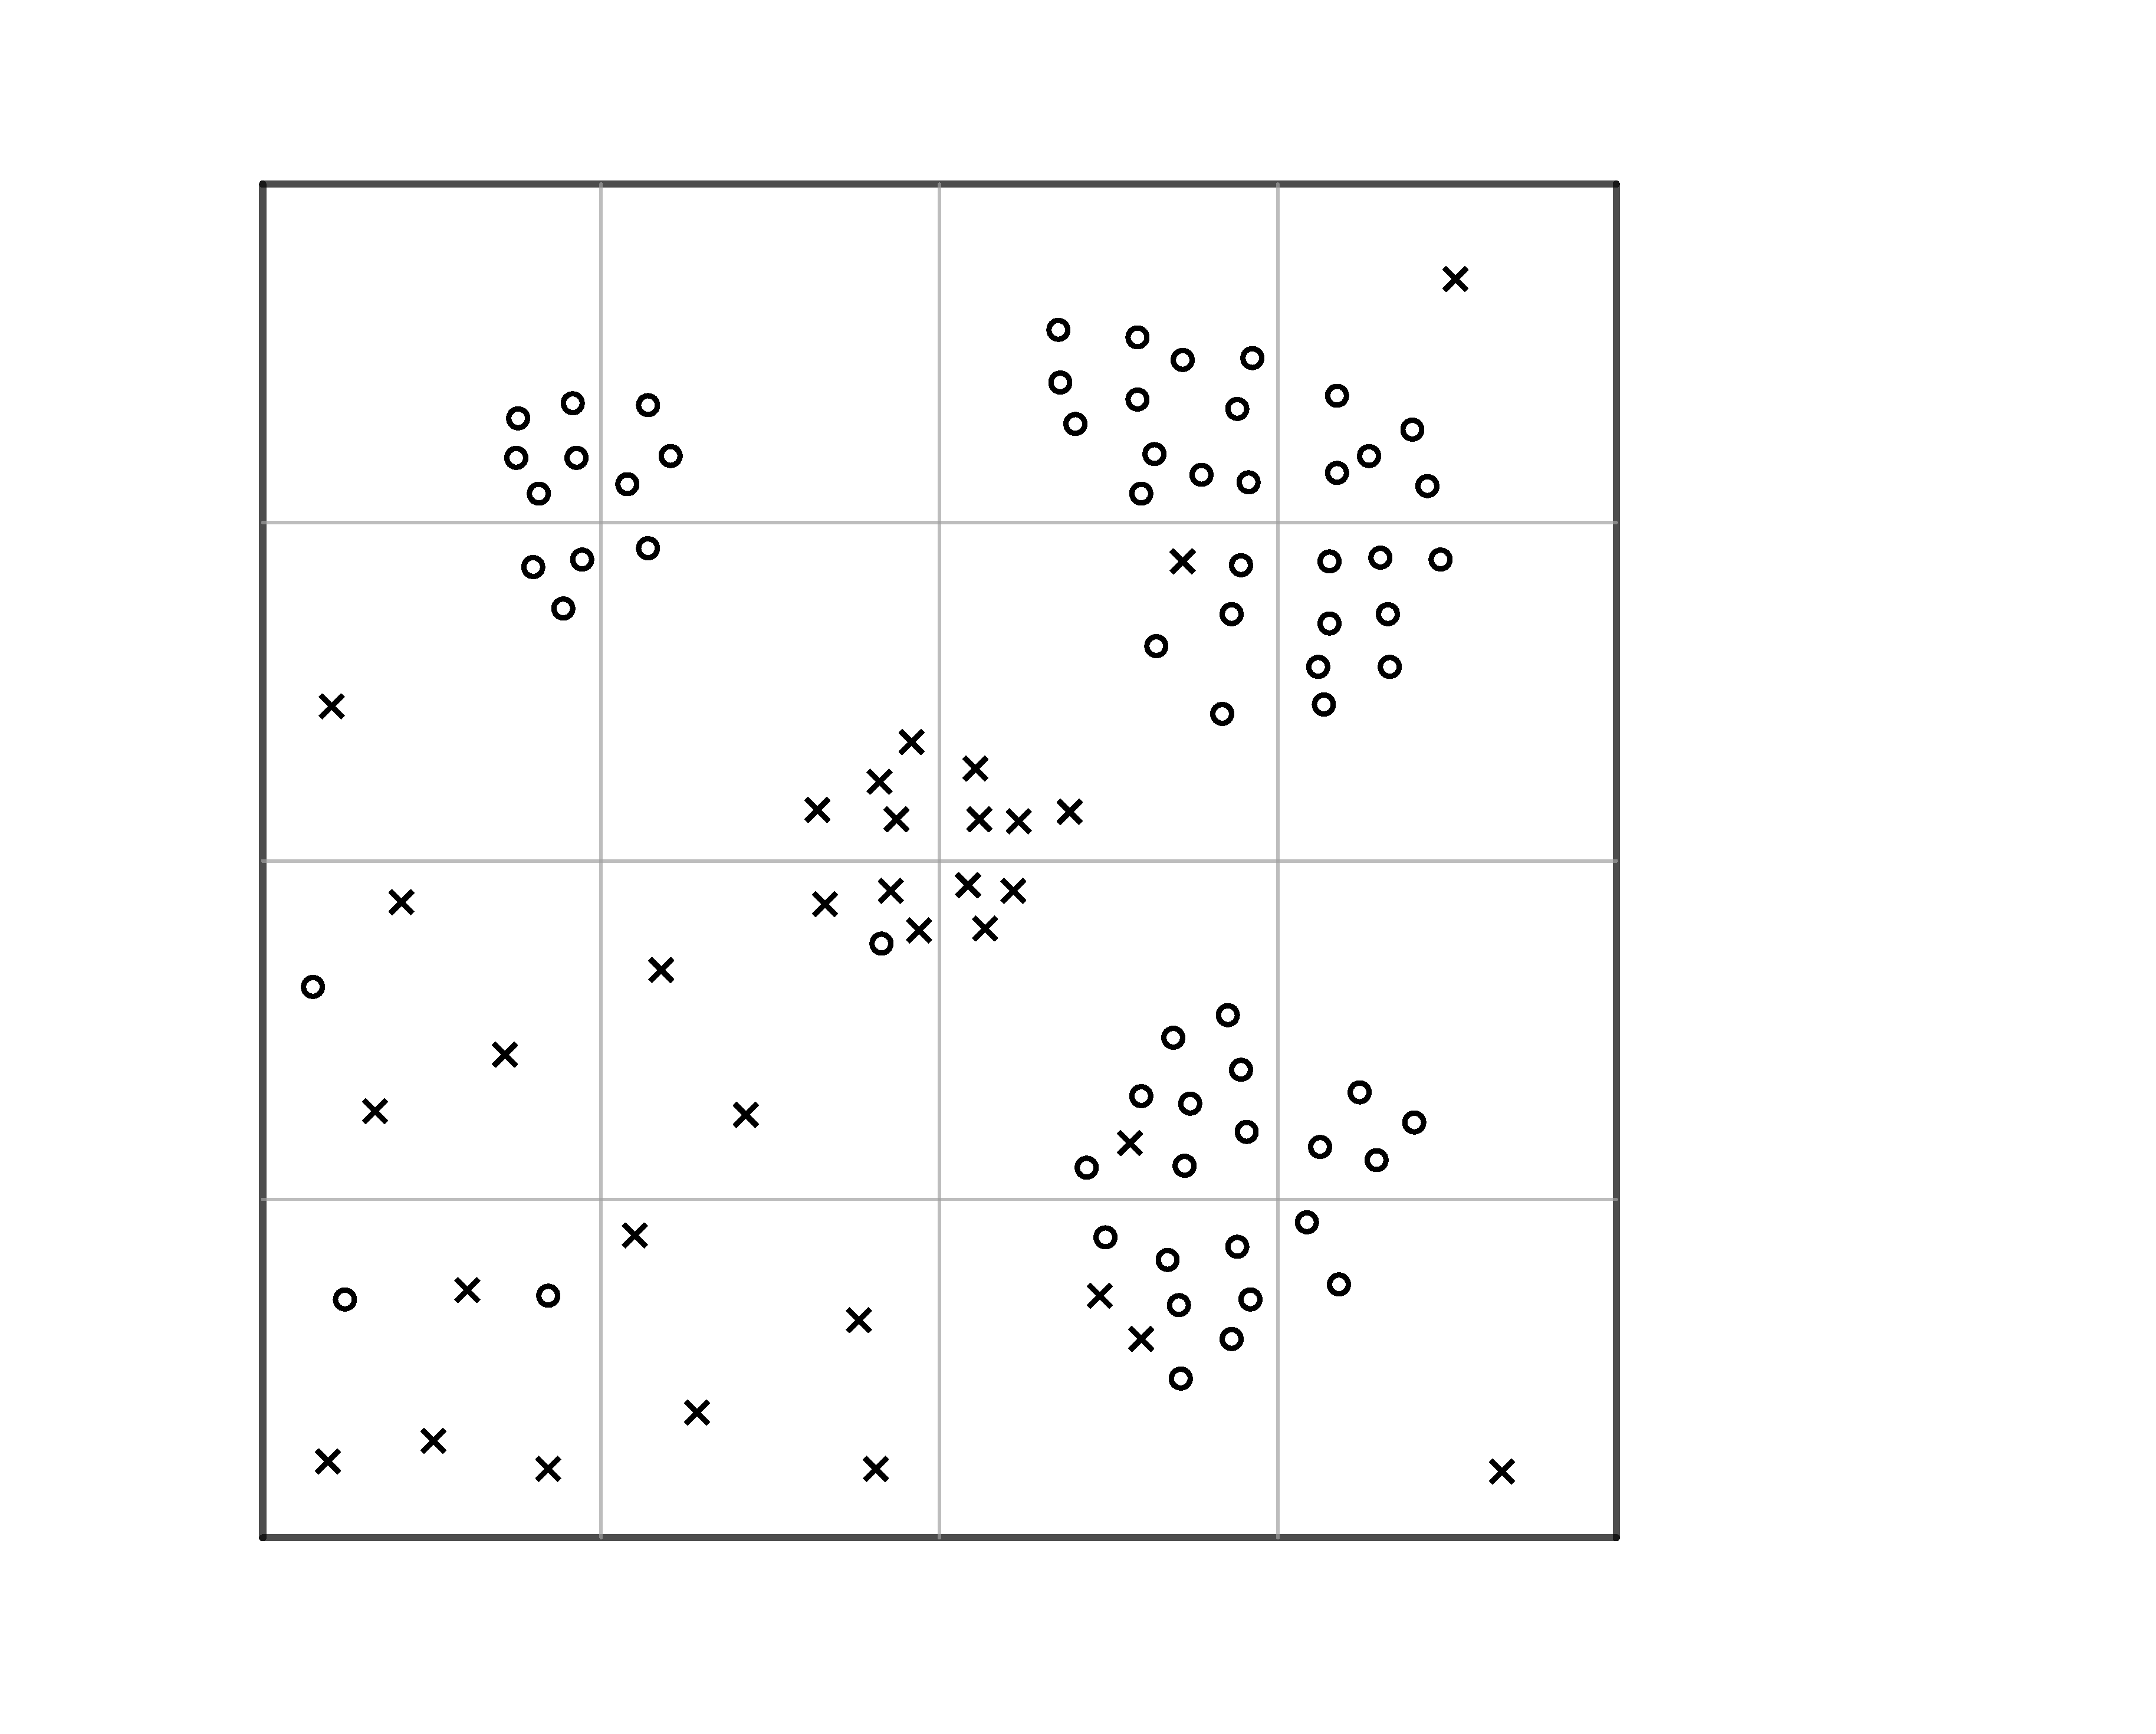
\includegraphics[width=1in]{assets/Gerrymandering/Gerry4x4-100-2.pdf} &  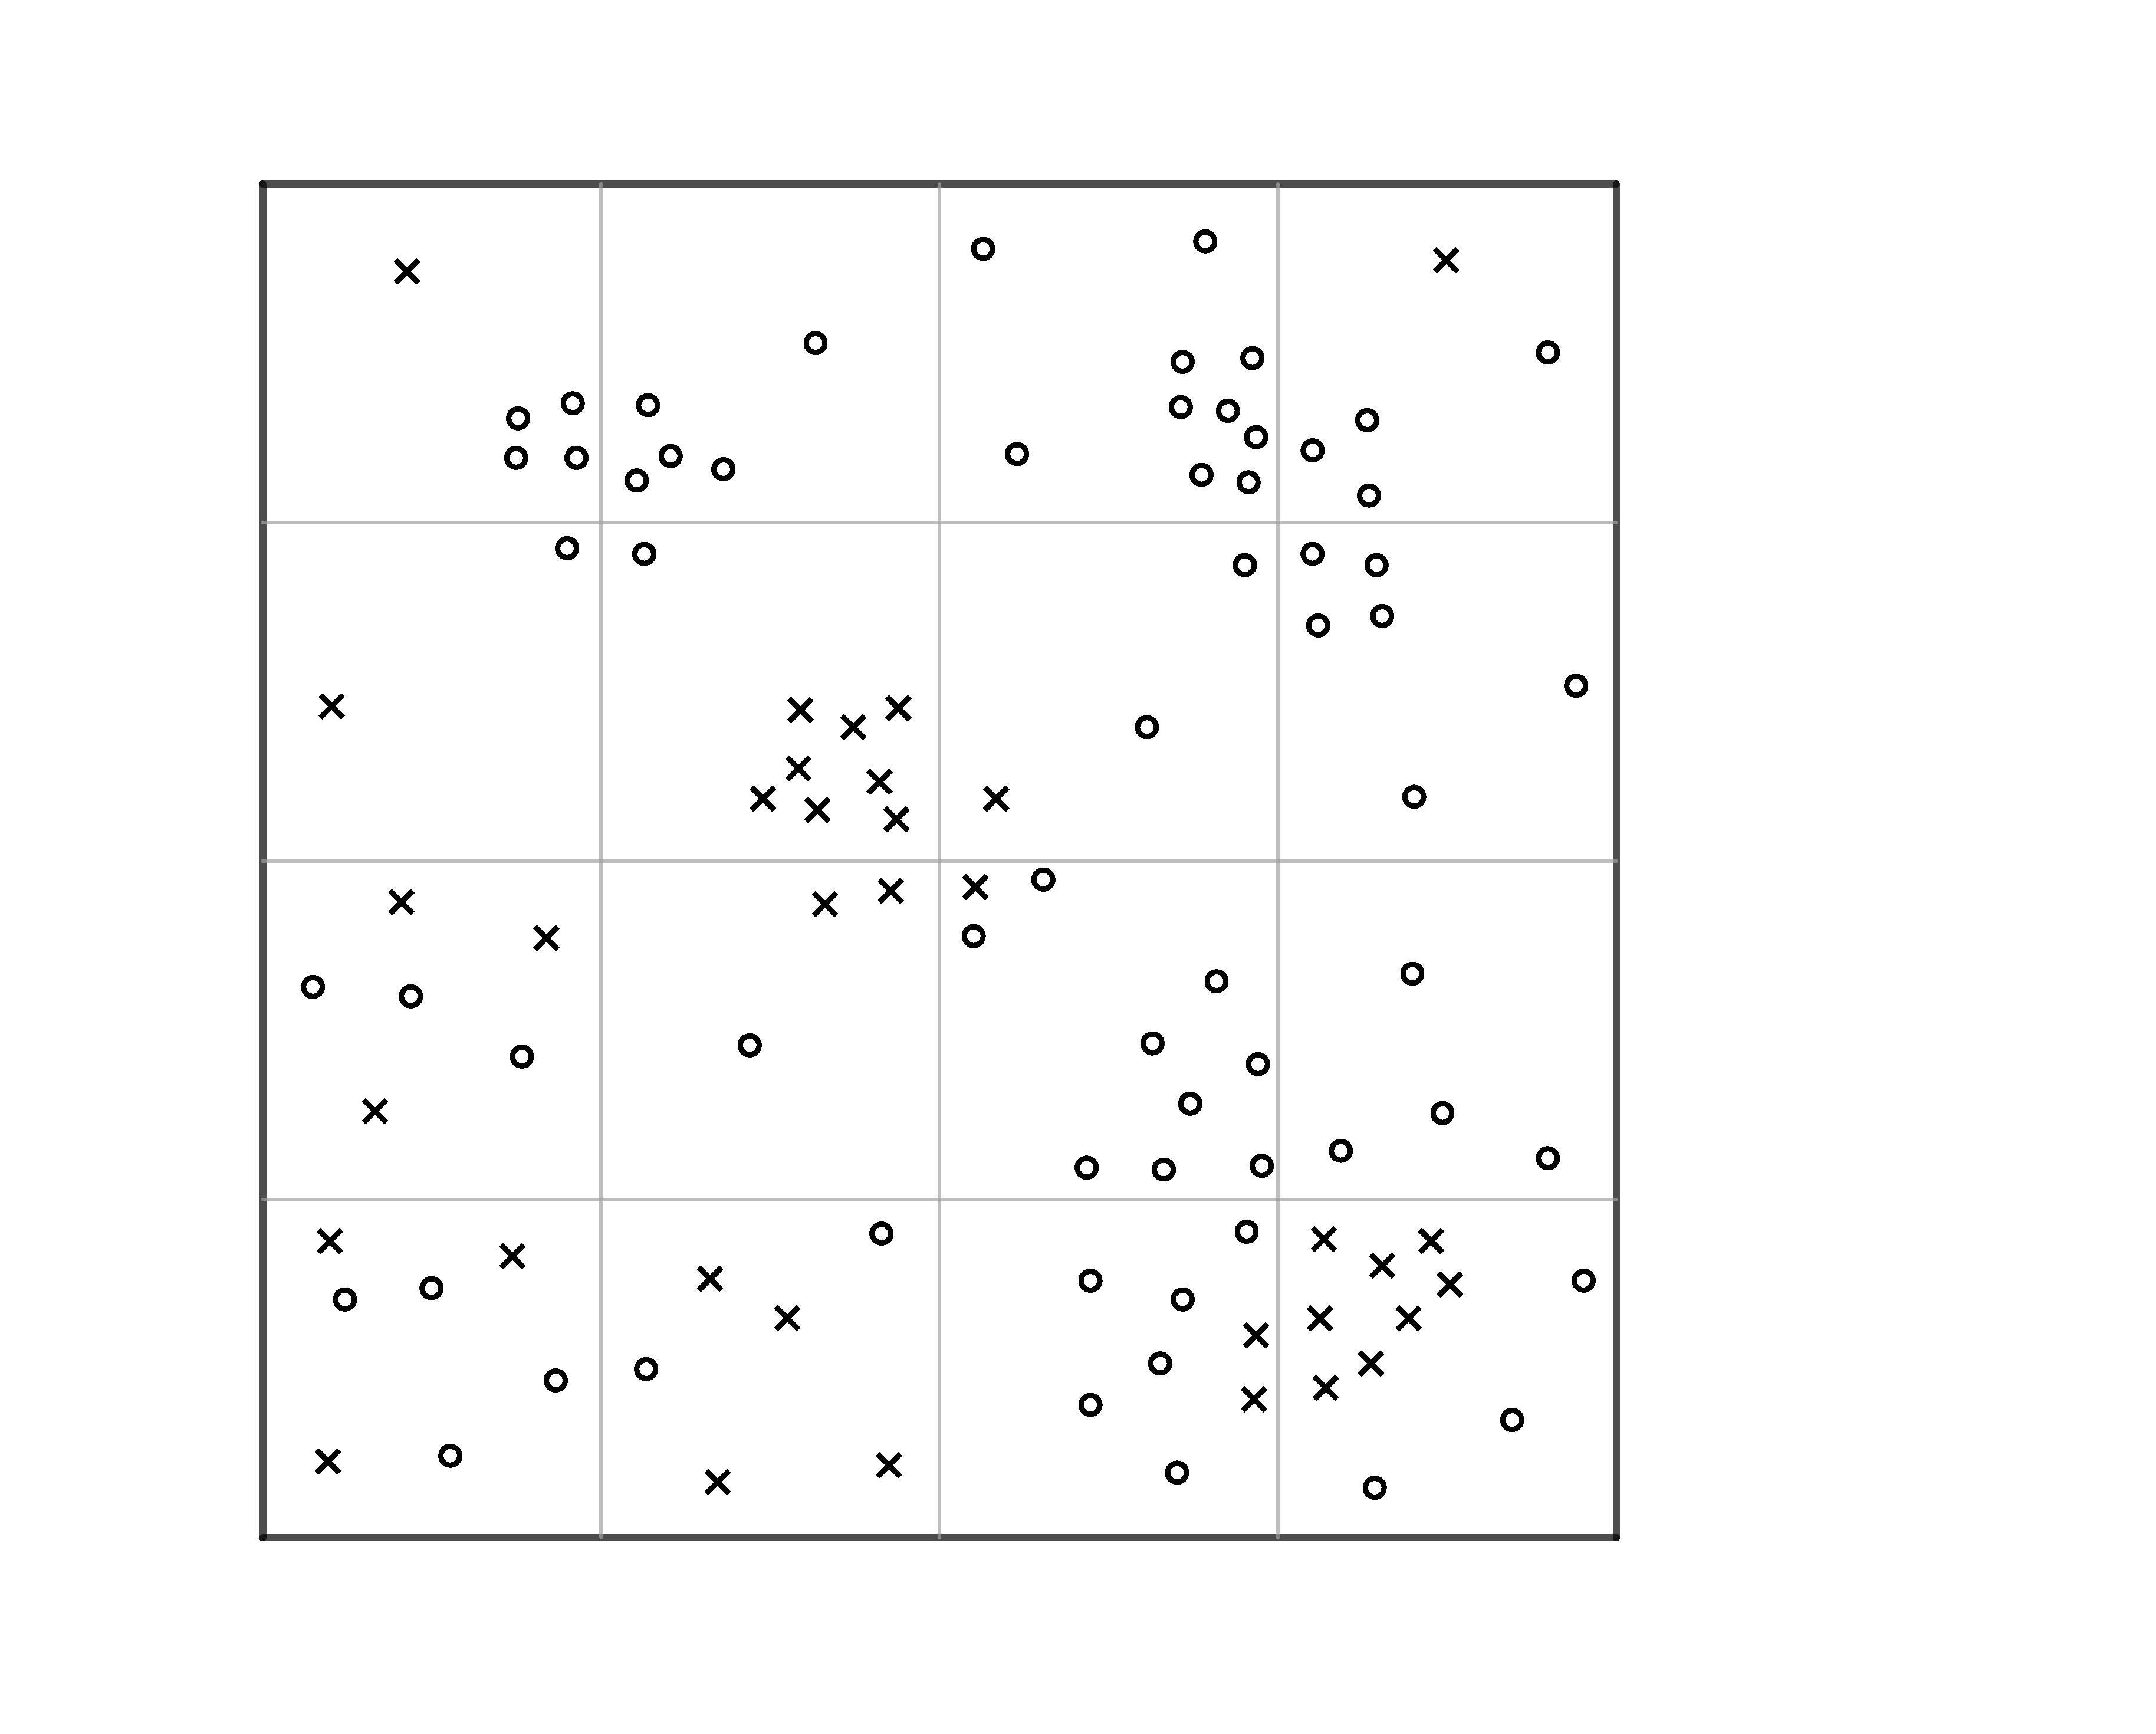
\includegraphics[width=1in]{assets/Gerrymandering/Gerry4x4-100-3.pdf}\\
% Total Vote Count &  Total Vote Count &  Total Vote Count\\
% X -  31& X - 34 & X  - 35\\
% O - 69 & O - 66 & O - 65
% \end{tabular}
%
%\begin{tabular}{c c c }
%
%Year 1 & Year 2 & Year 3 \\
% 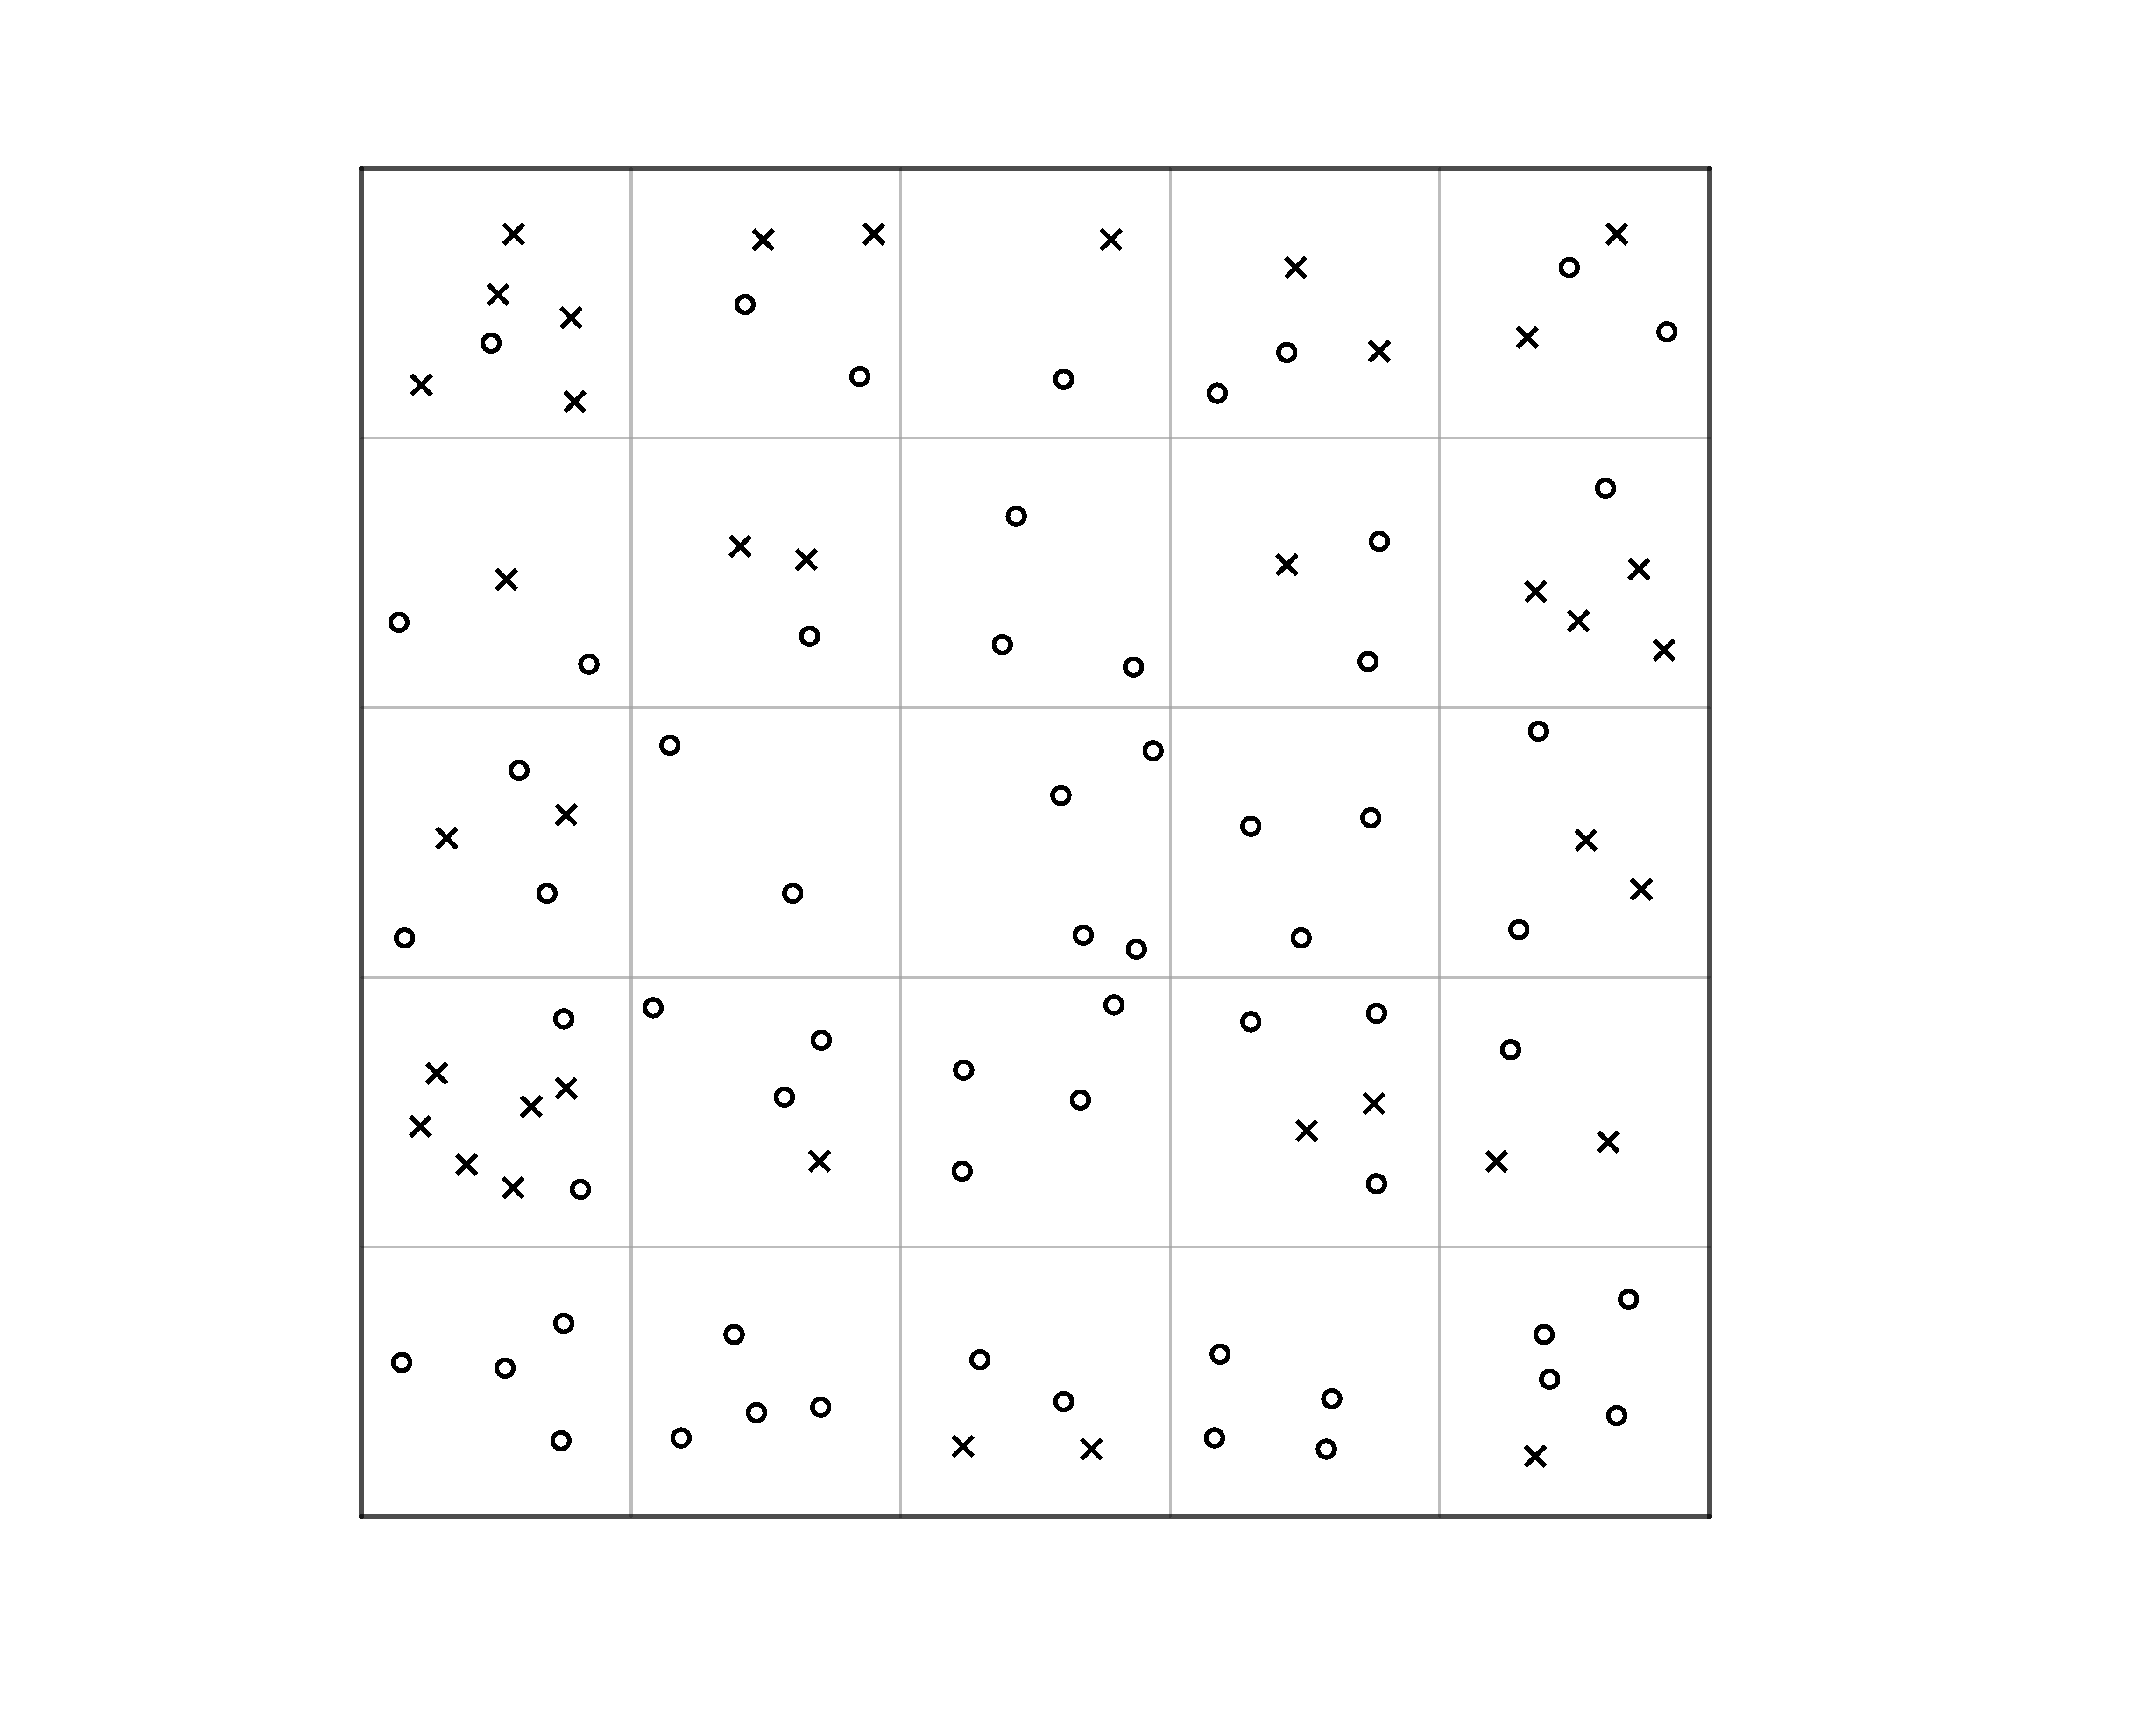
\includegraphics[width=1in]{assets/Gerrymandering/Gerry5x5-100-1.pdf} &  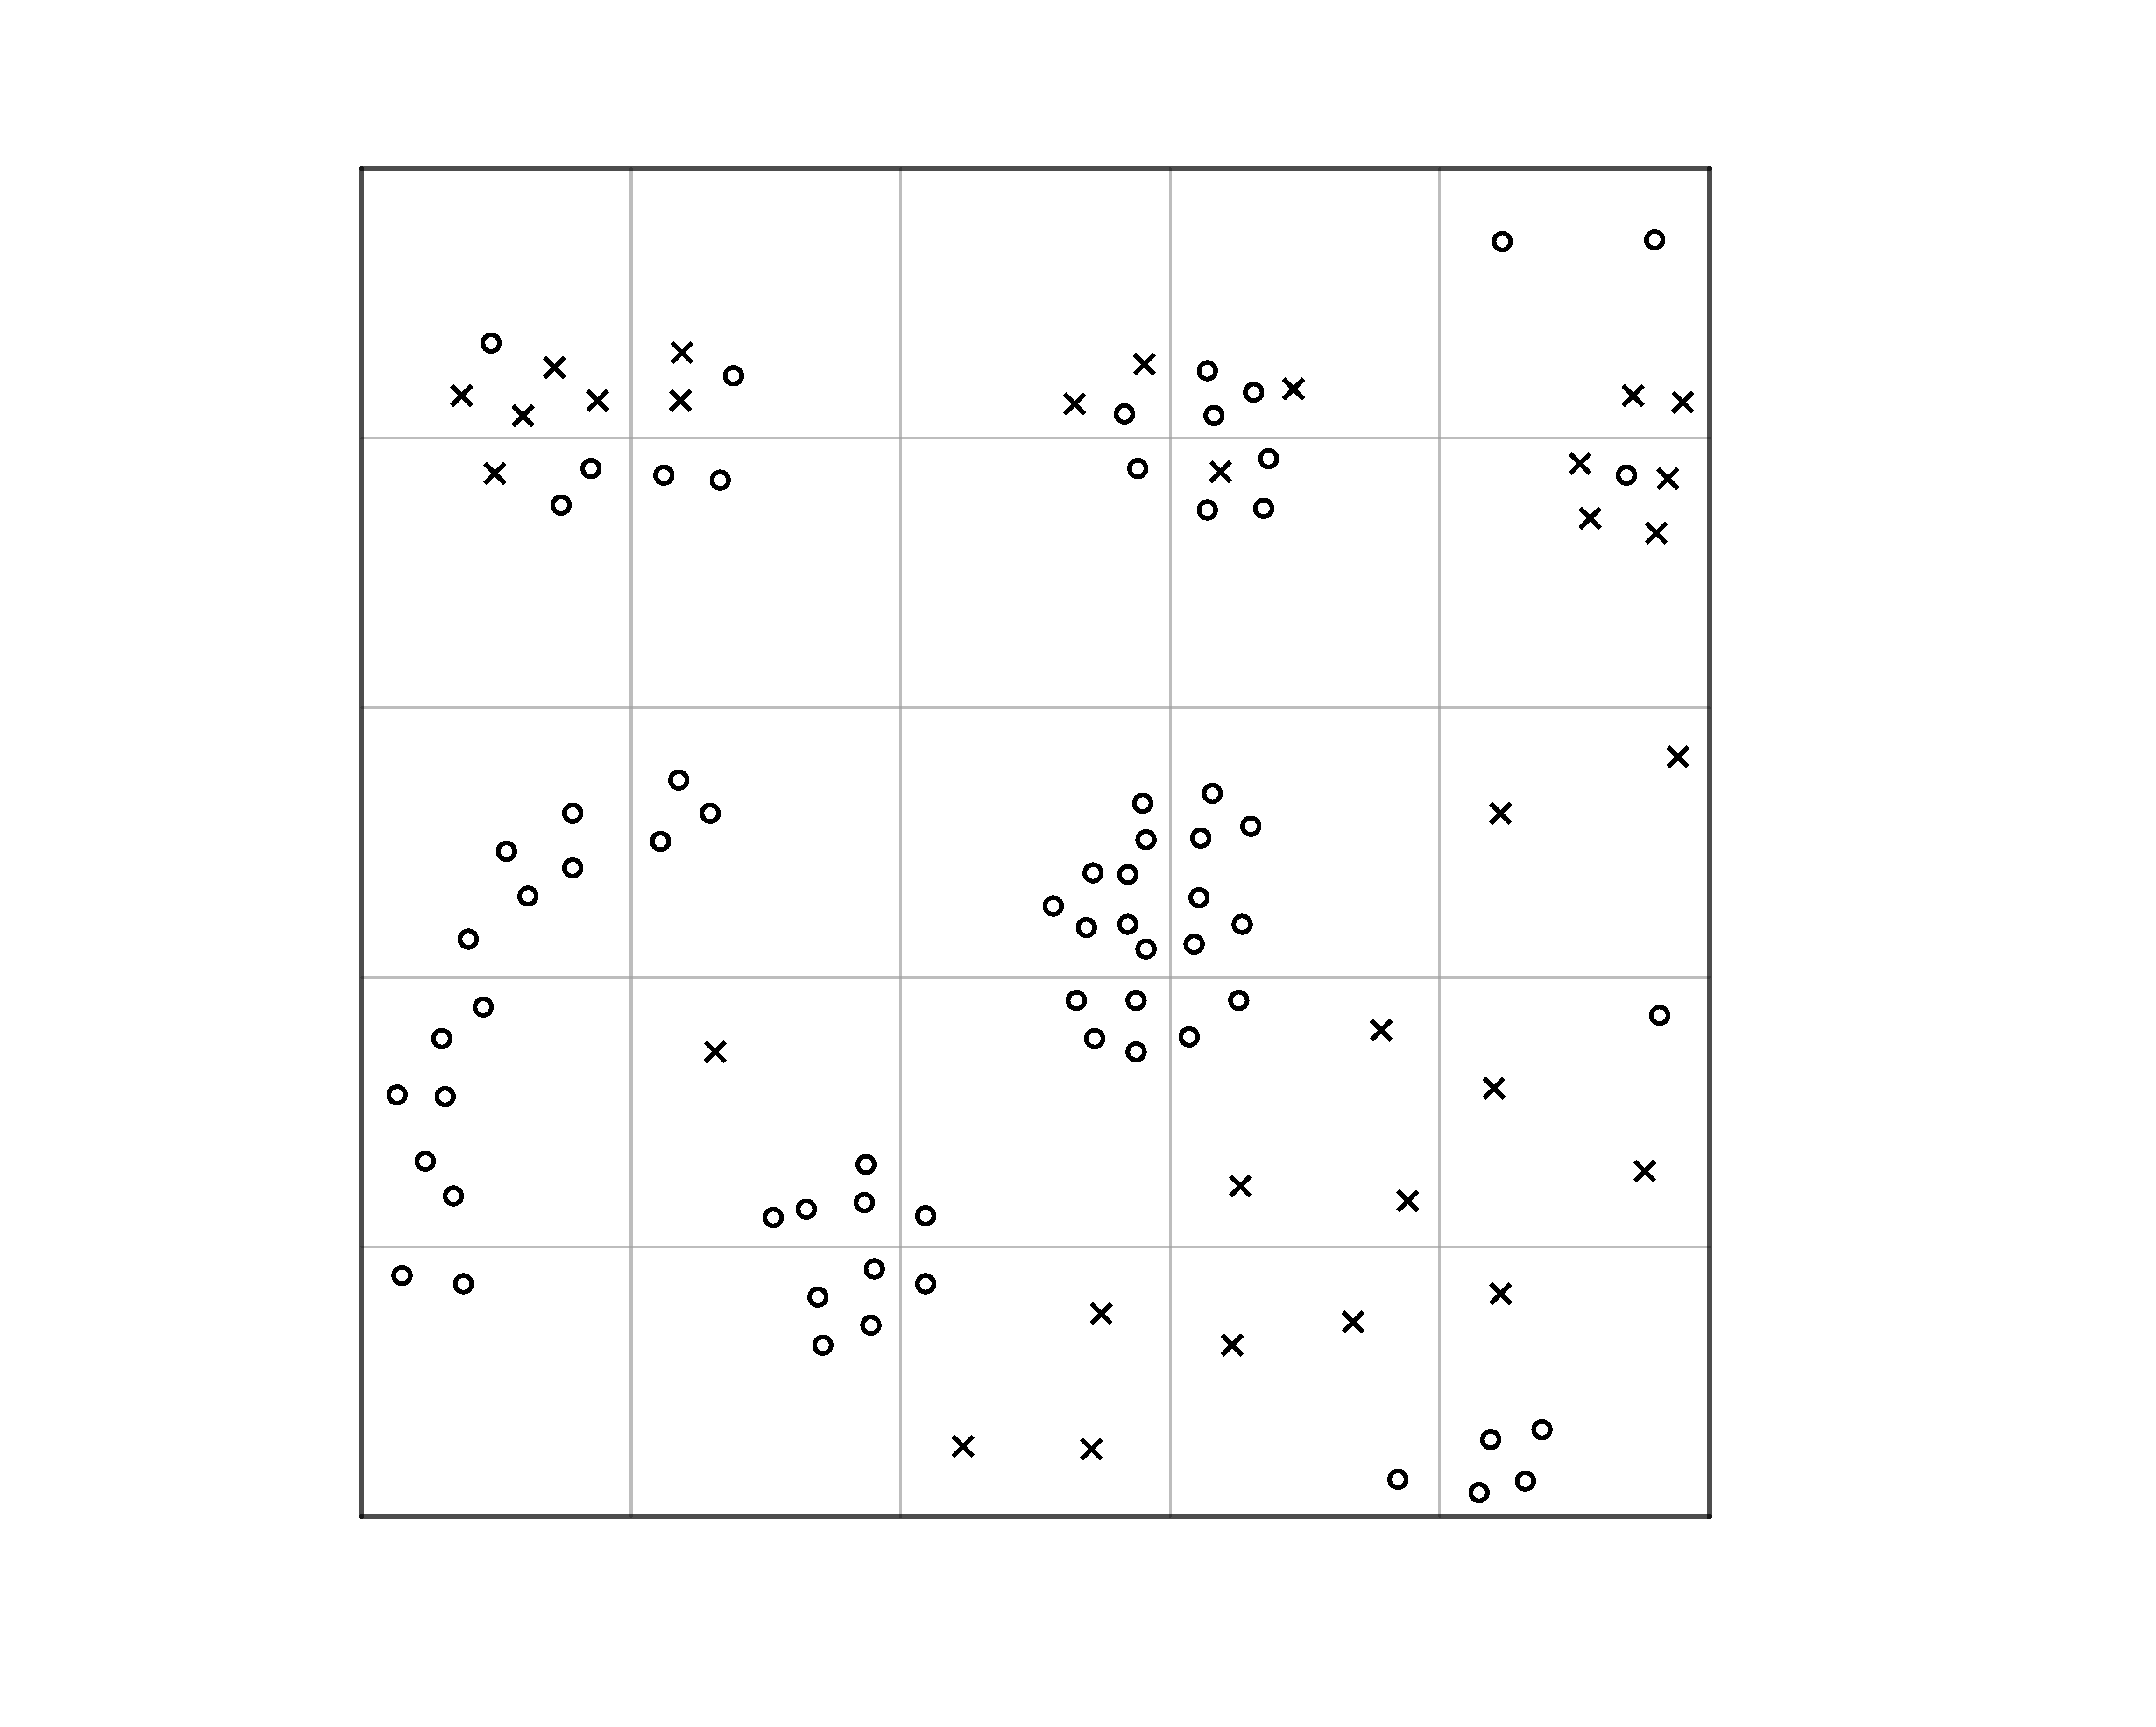
\includegraphics[width=1in]{assets/Gerrymandering/Gerry5x5-100-2.pdf} &  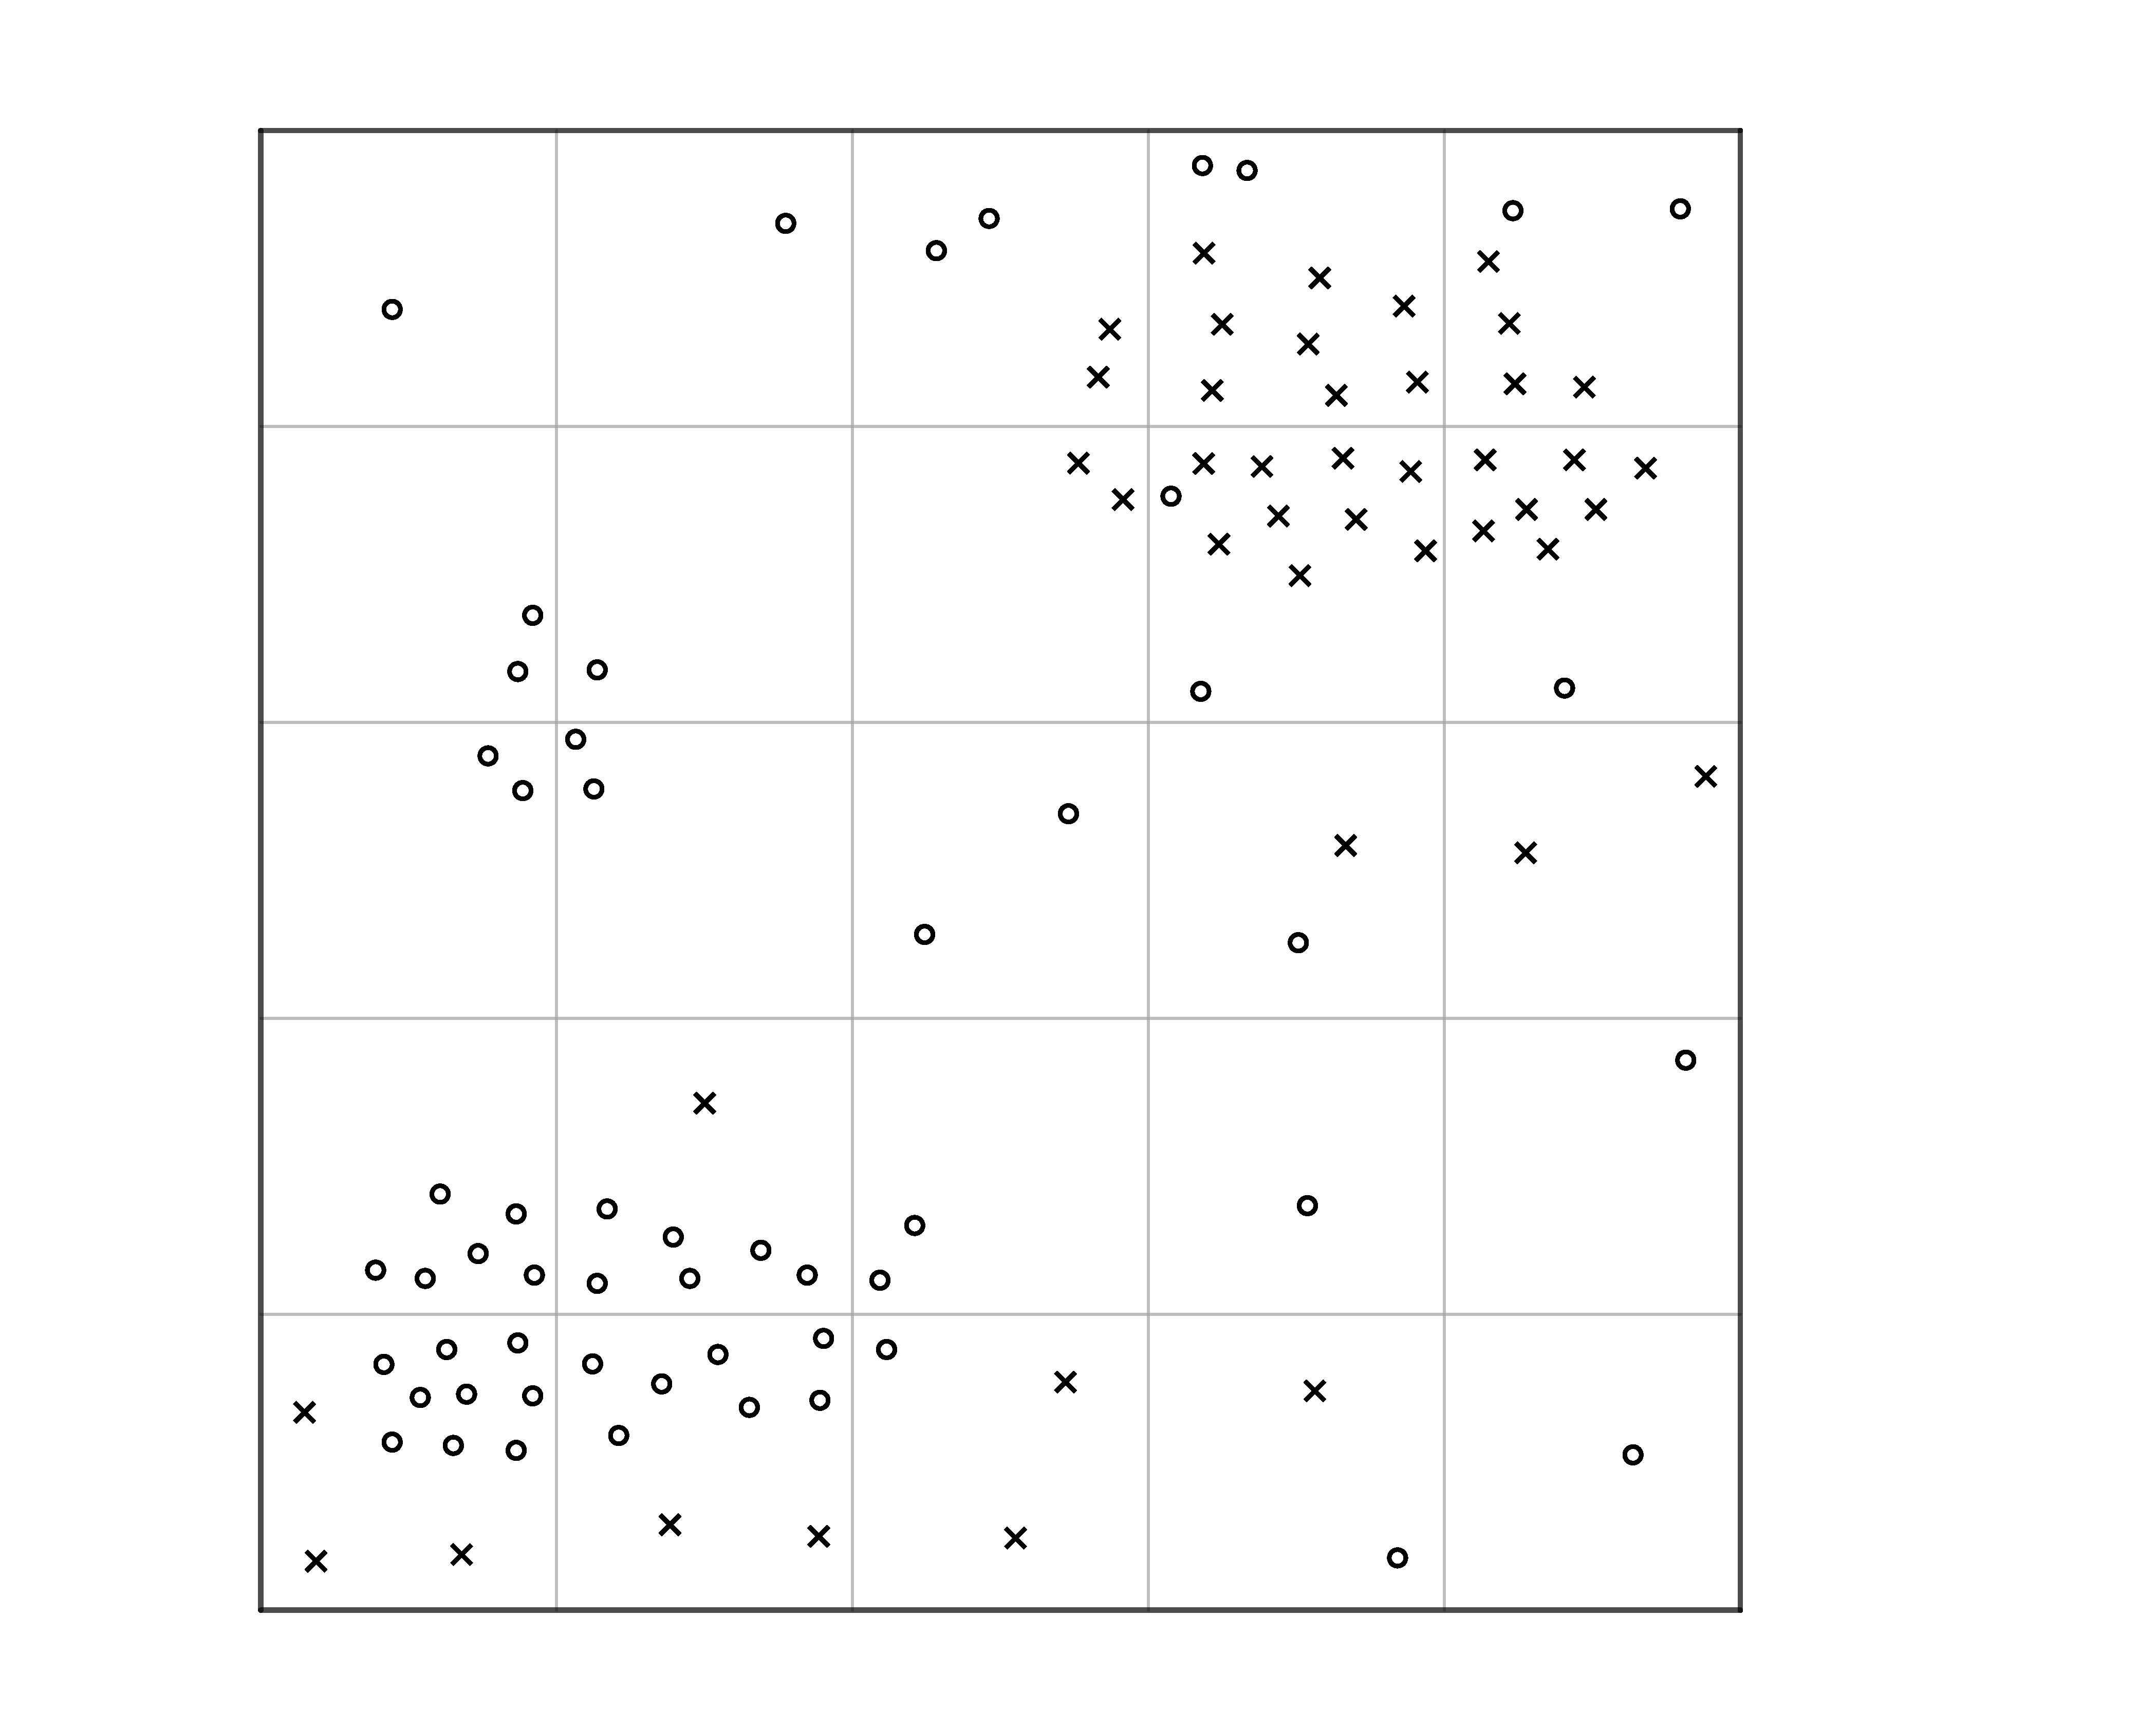
\includegraphics[width=1in]{assets/Gerrymandering/Gerry5x5-100-3.pdf}\\
% Total Vote Count &  Total Vote Count &  Total Vote Count\\
% X -  38& X - 31 & X  - 44\\
% O - 62 & O - 69 & O - 56
% \end{tabular}
%\begin{tabular}{c c c }
%
%Year 1 & Year 2 & Year 3 \\
% 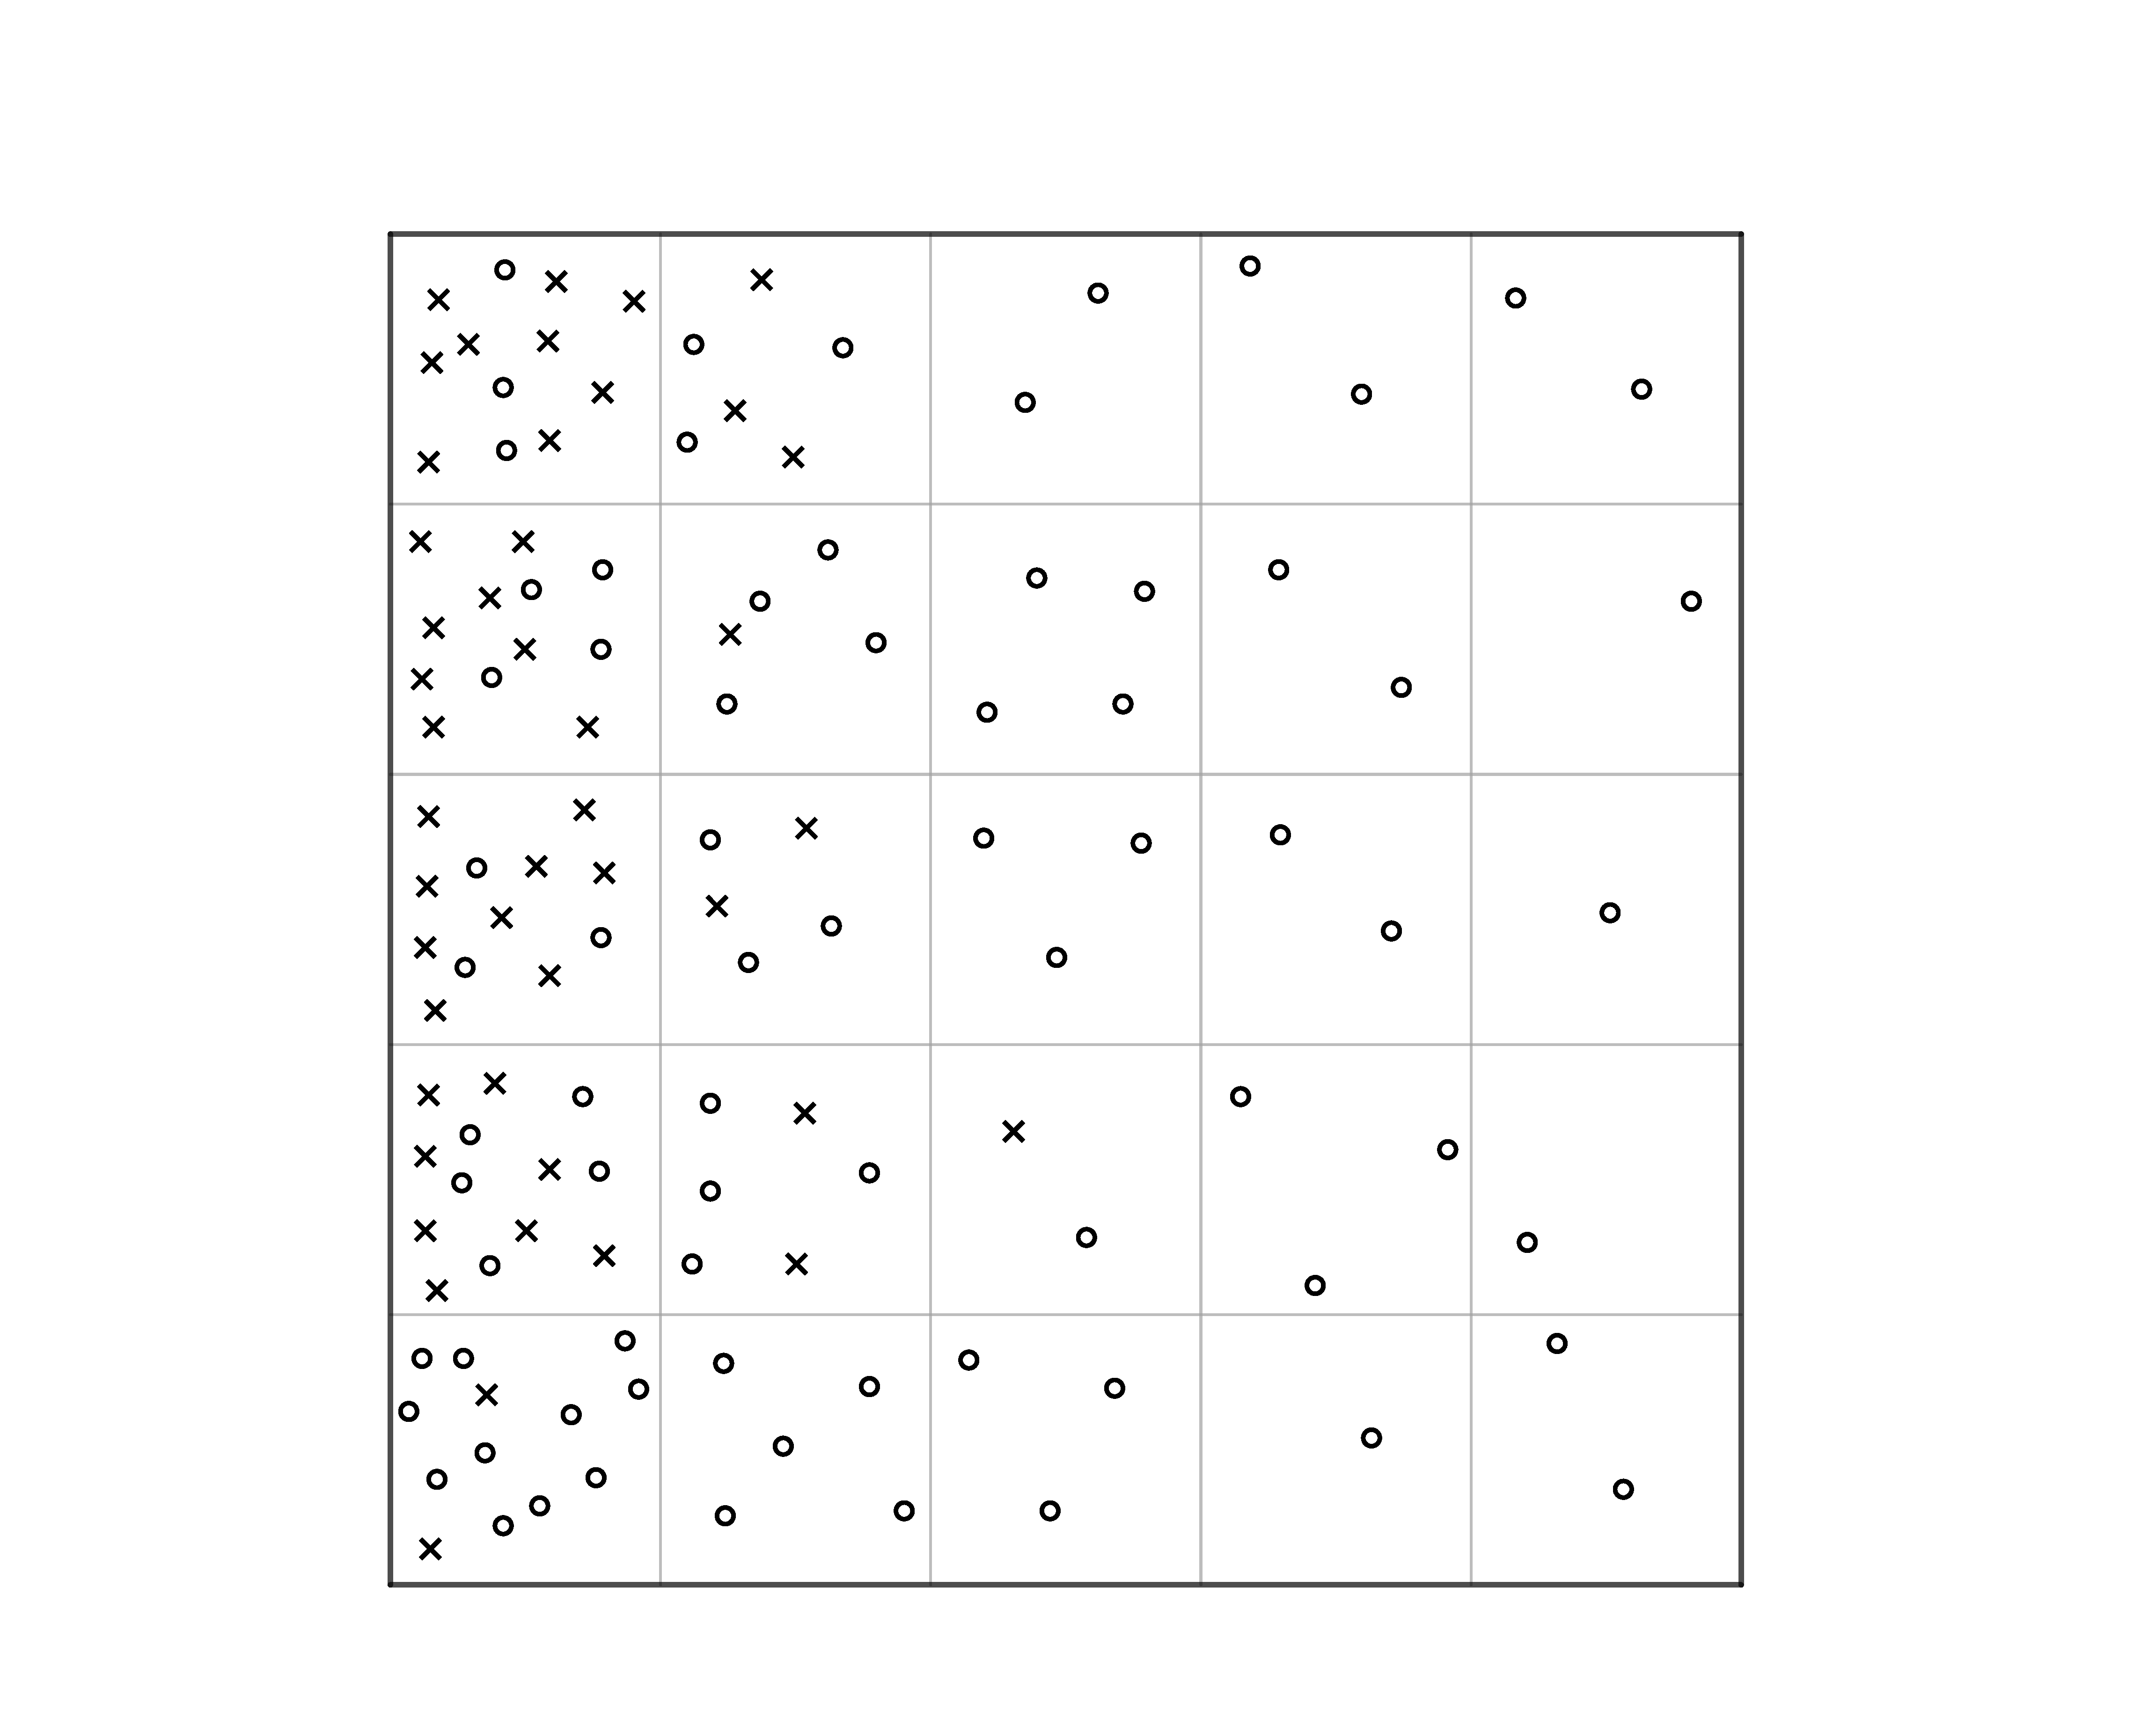
\includegraphics[width=1in]{assets/Gerrymandering/Gerry5x5-120-1.pdf} &  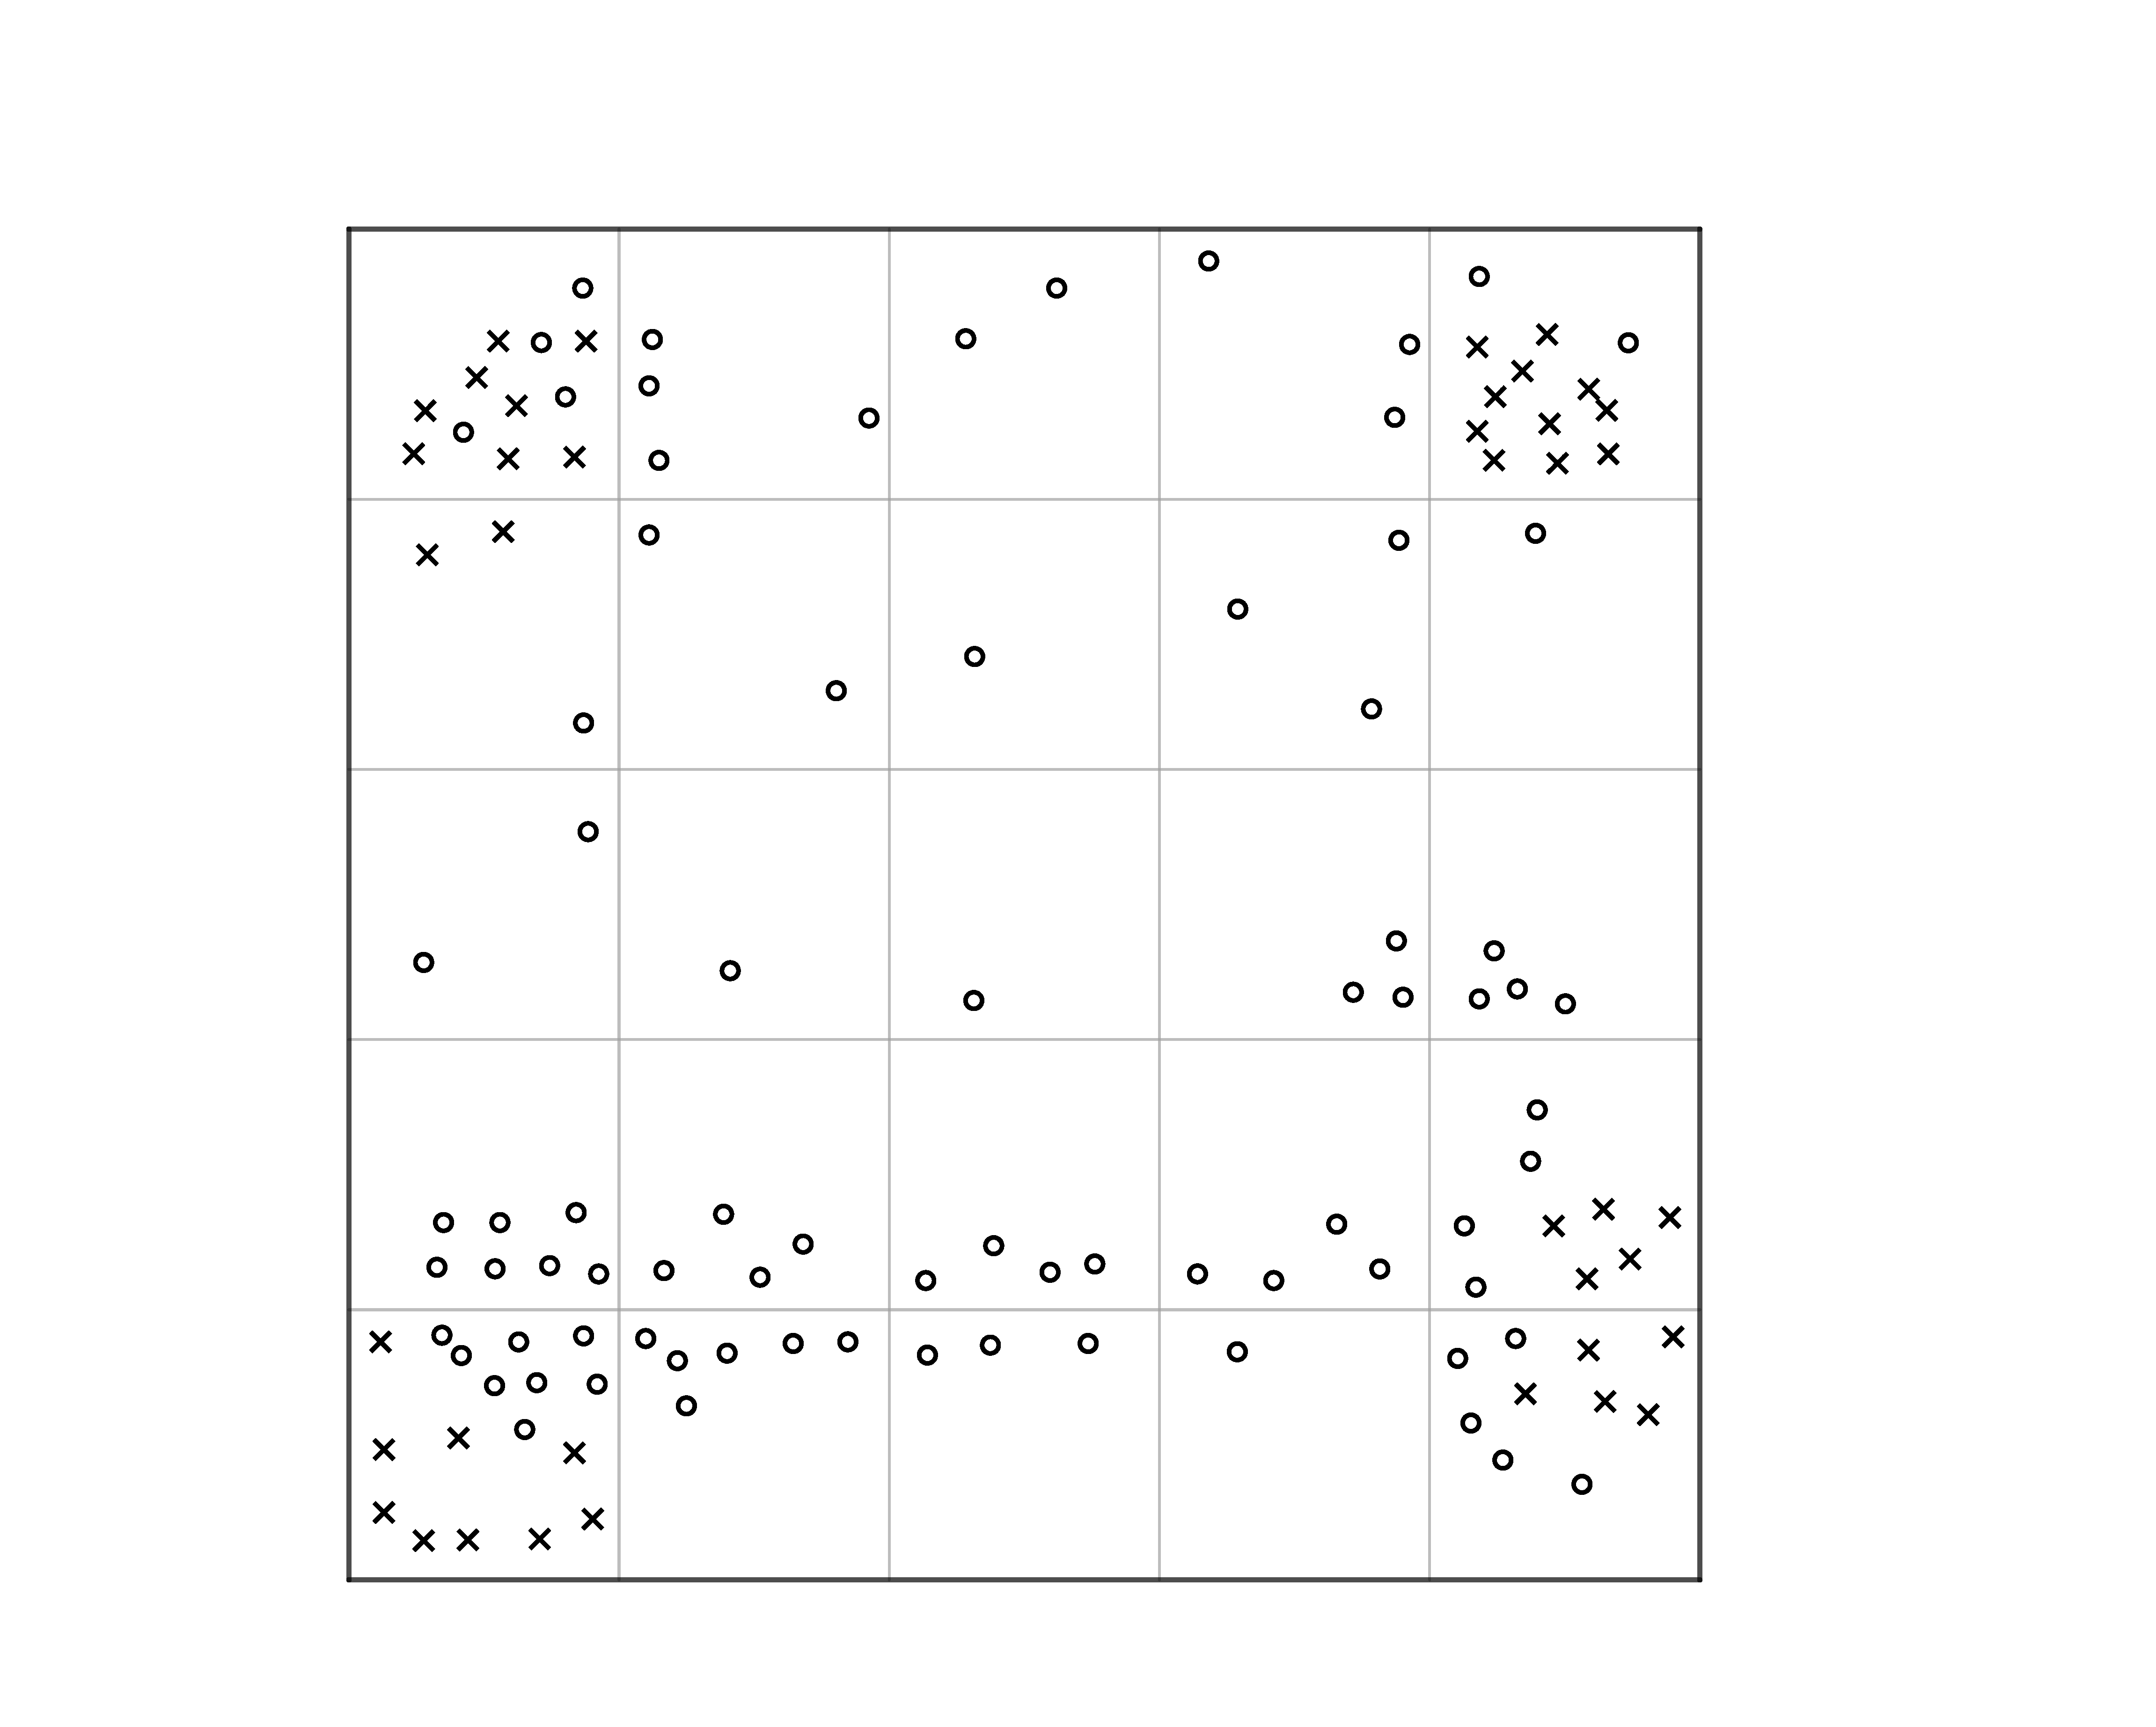
\includegraphics[width=1in]{assets/Gerrymandering/Gerry5x5-120-2.pdf} &  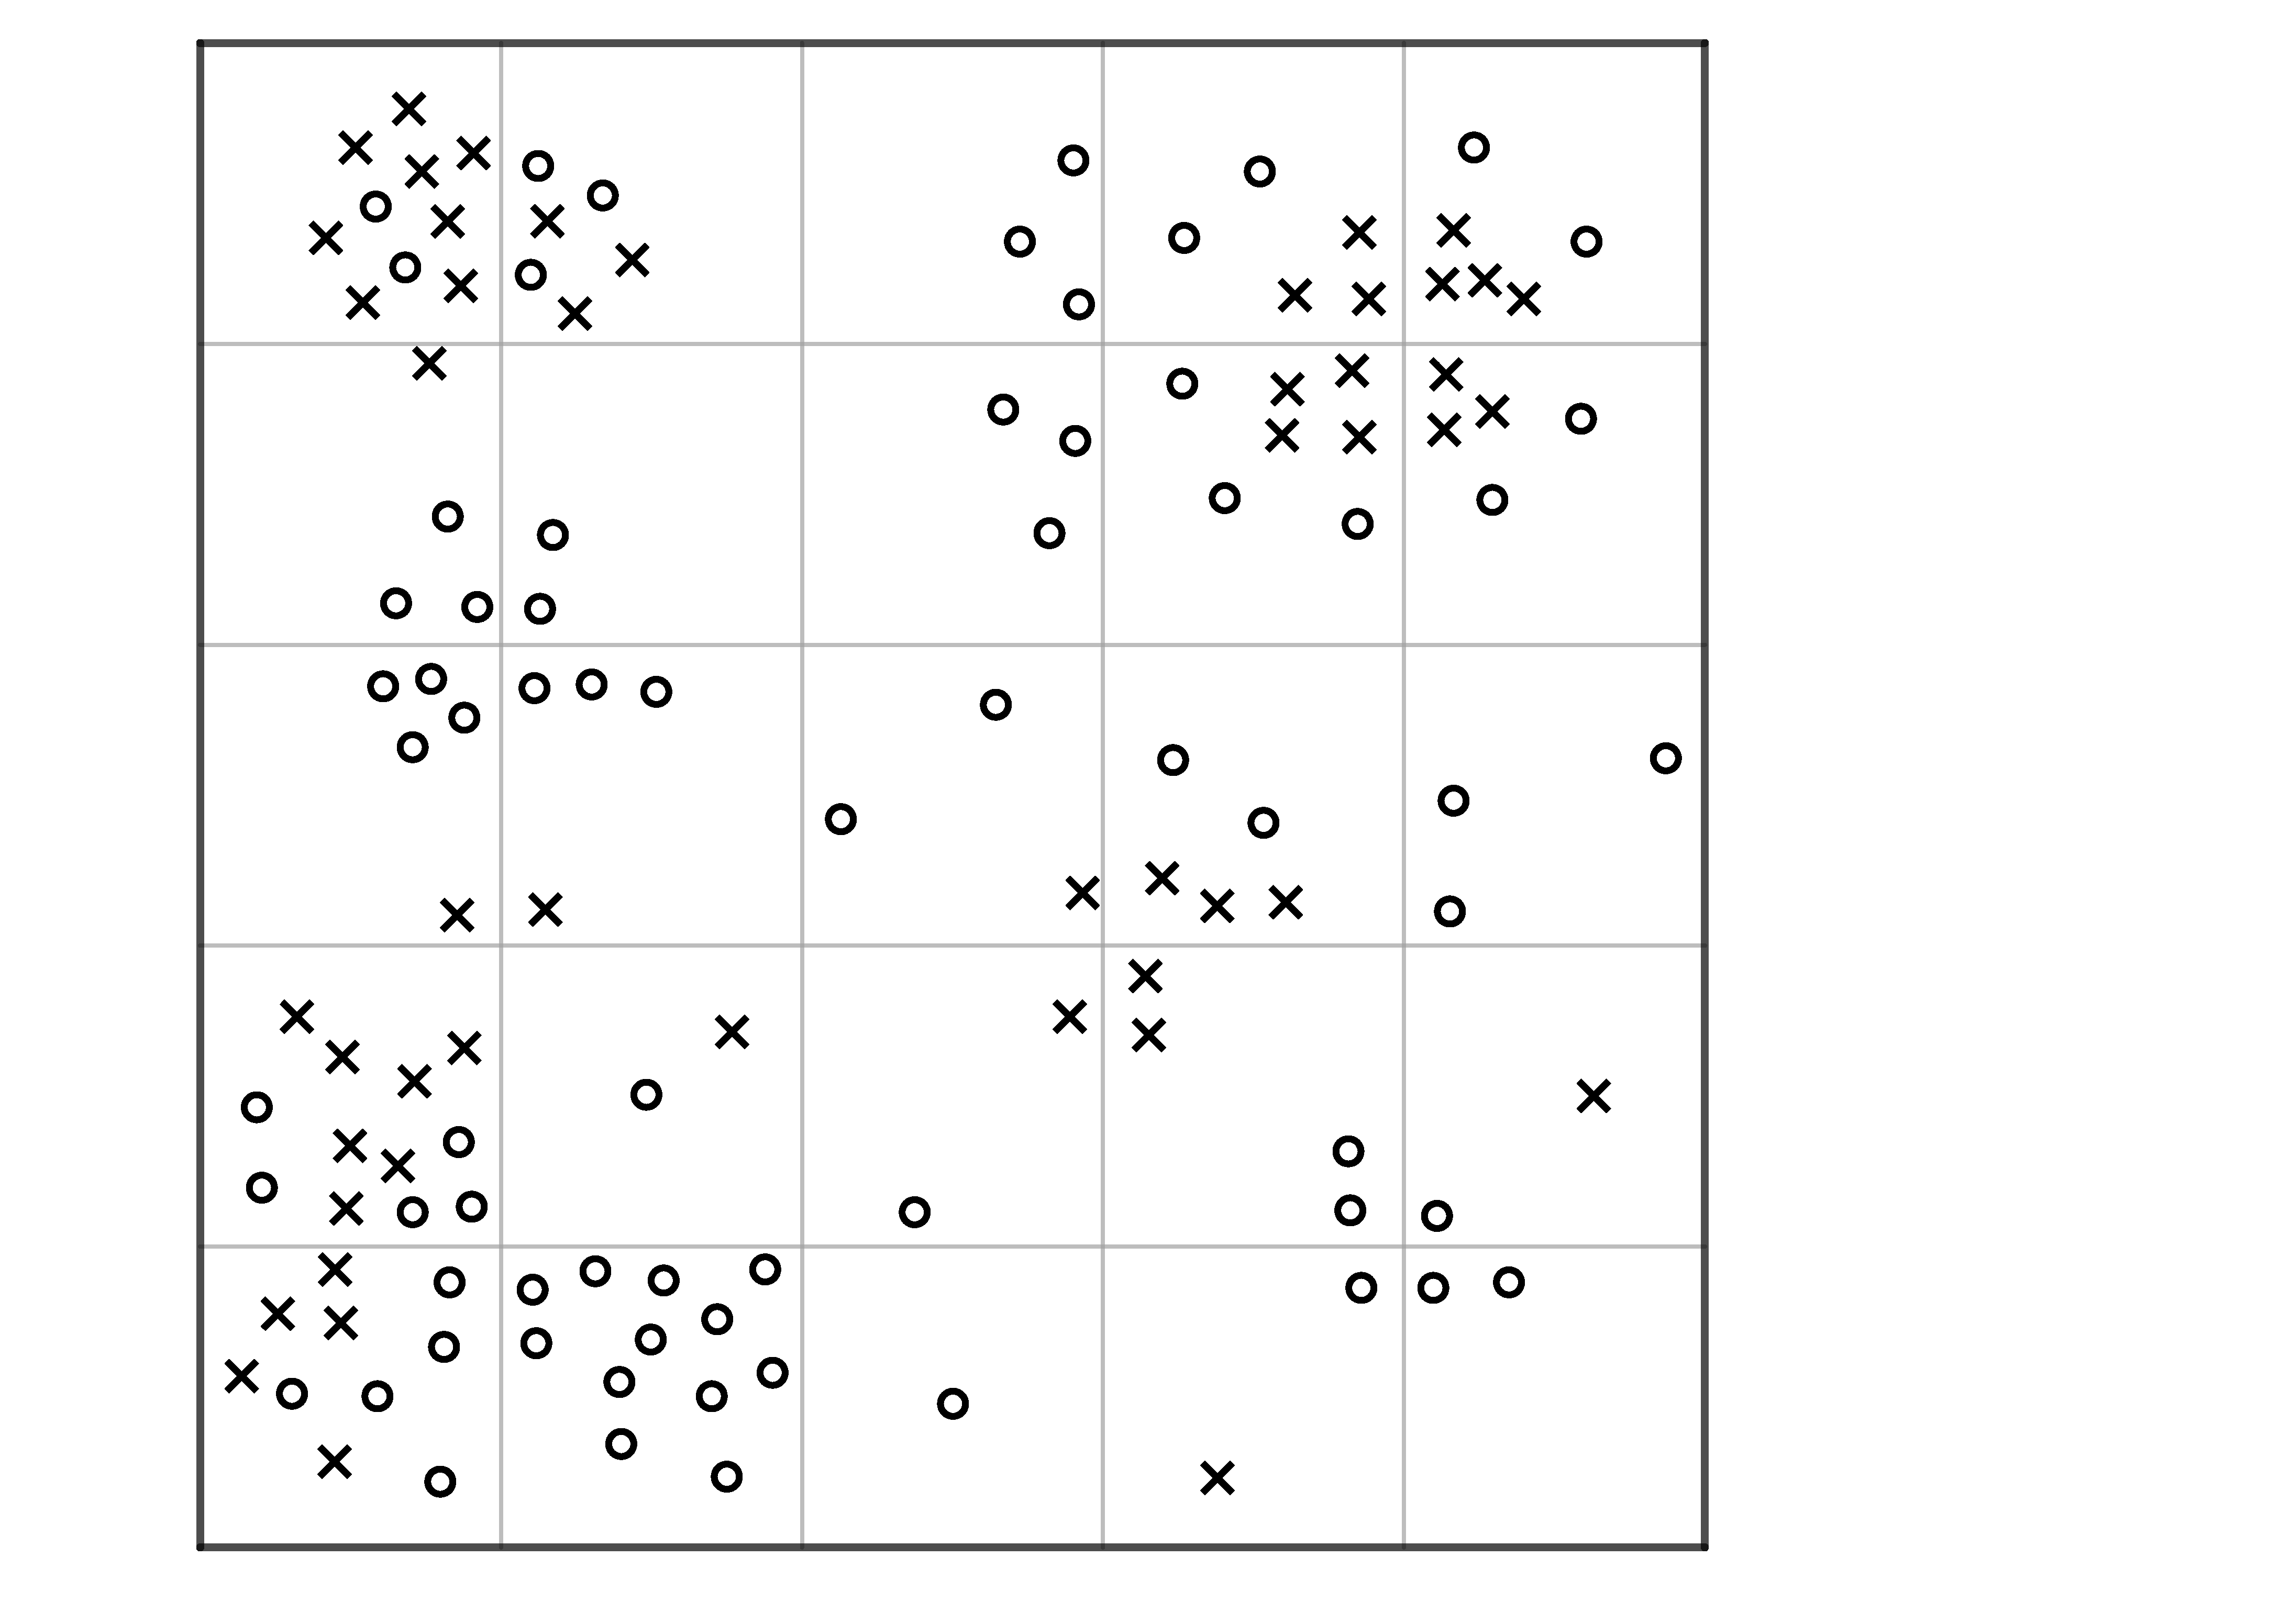
\includegraphics[width=1in]{assets/Gerrymandering/Gerry5x5-120-3.pdf}\\
% Total Vote Count &  Total Vote Count &  Total Vote Count\\
% X -  45& X - 40 & X  - 50\\
% O - 75 & O - 80 & O - 70
% \end{tabular}
%
%\begin{tabular}{c c c }
%
%Year 1 & Year 2 & Year 3 \\
% 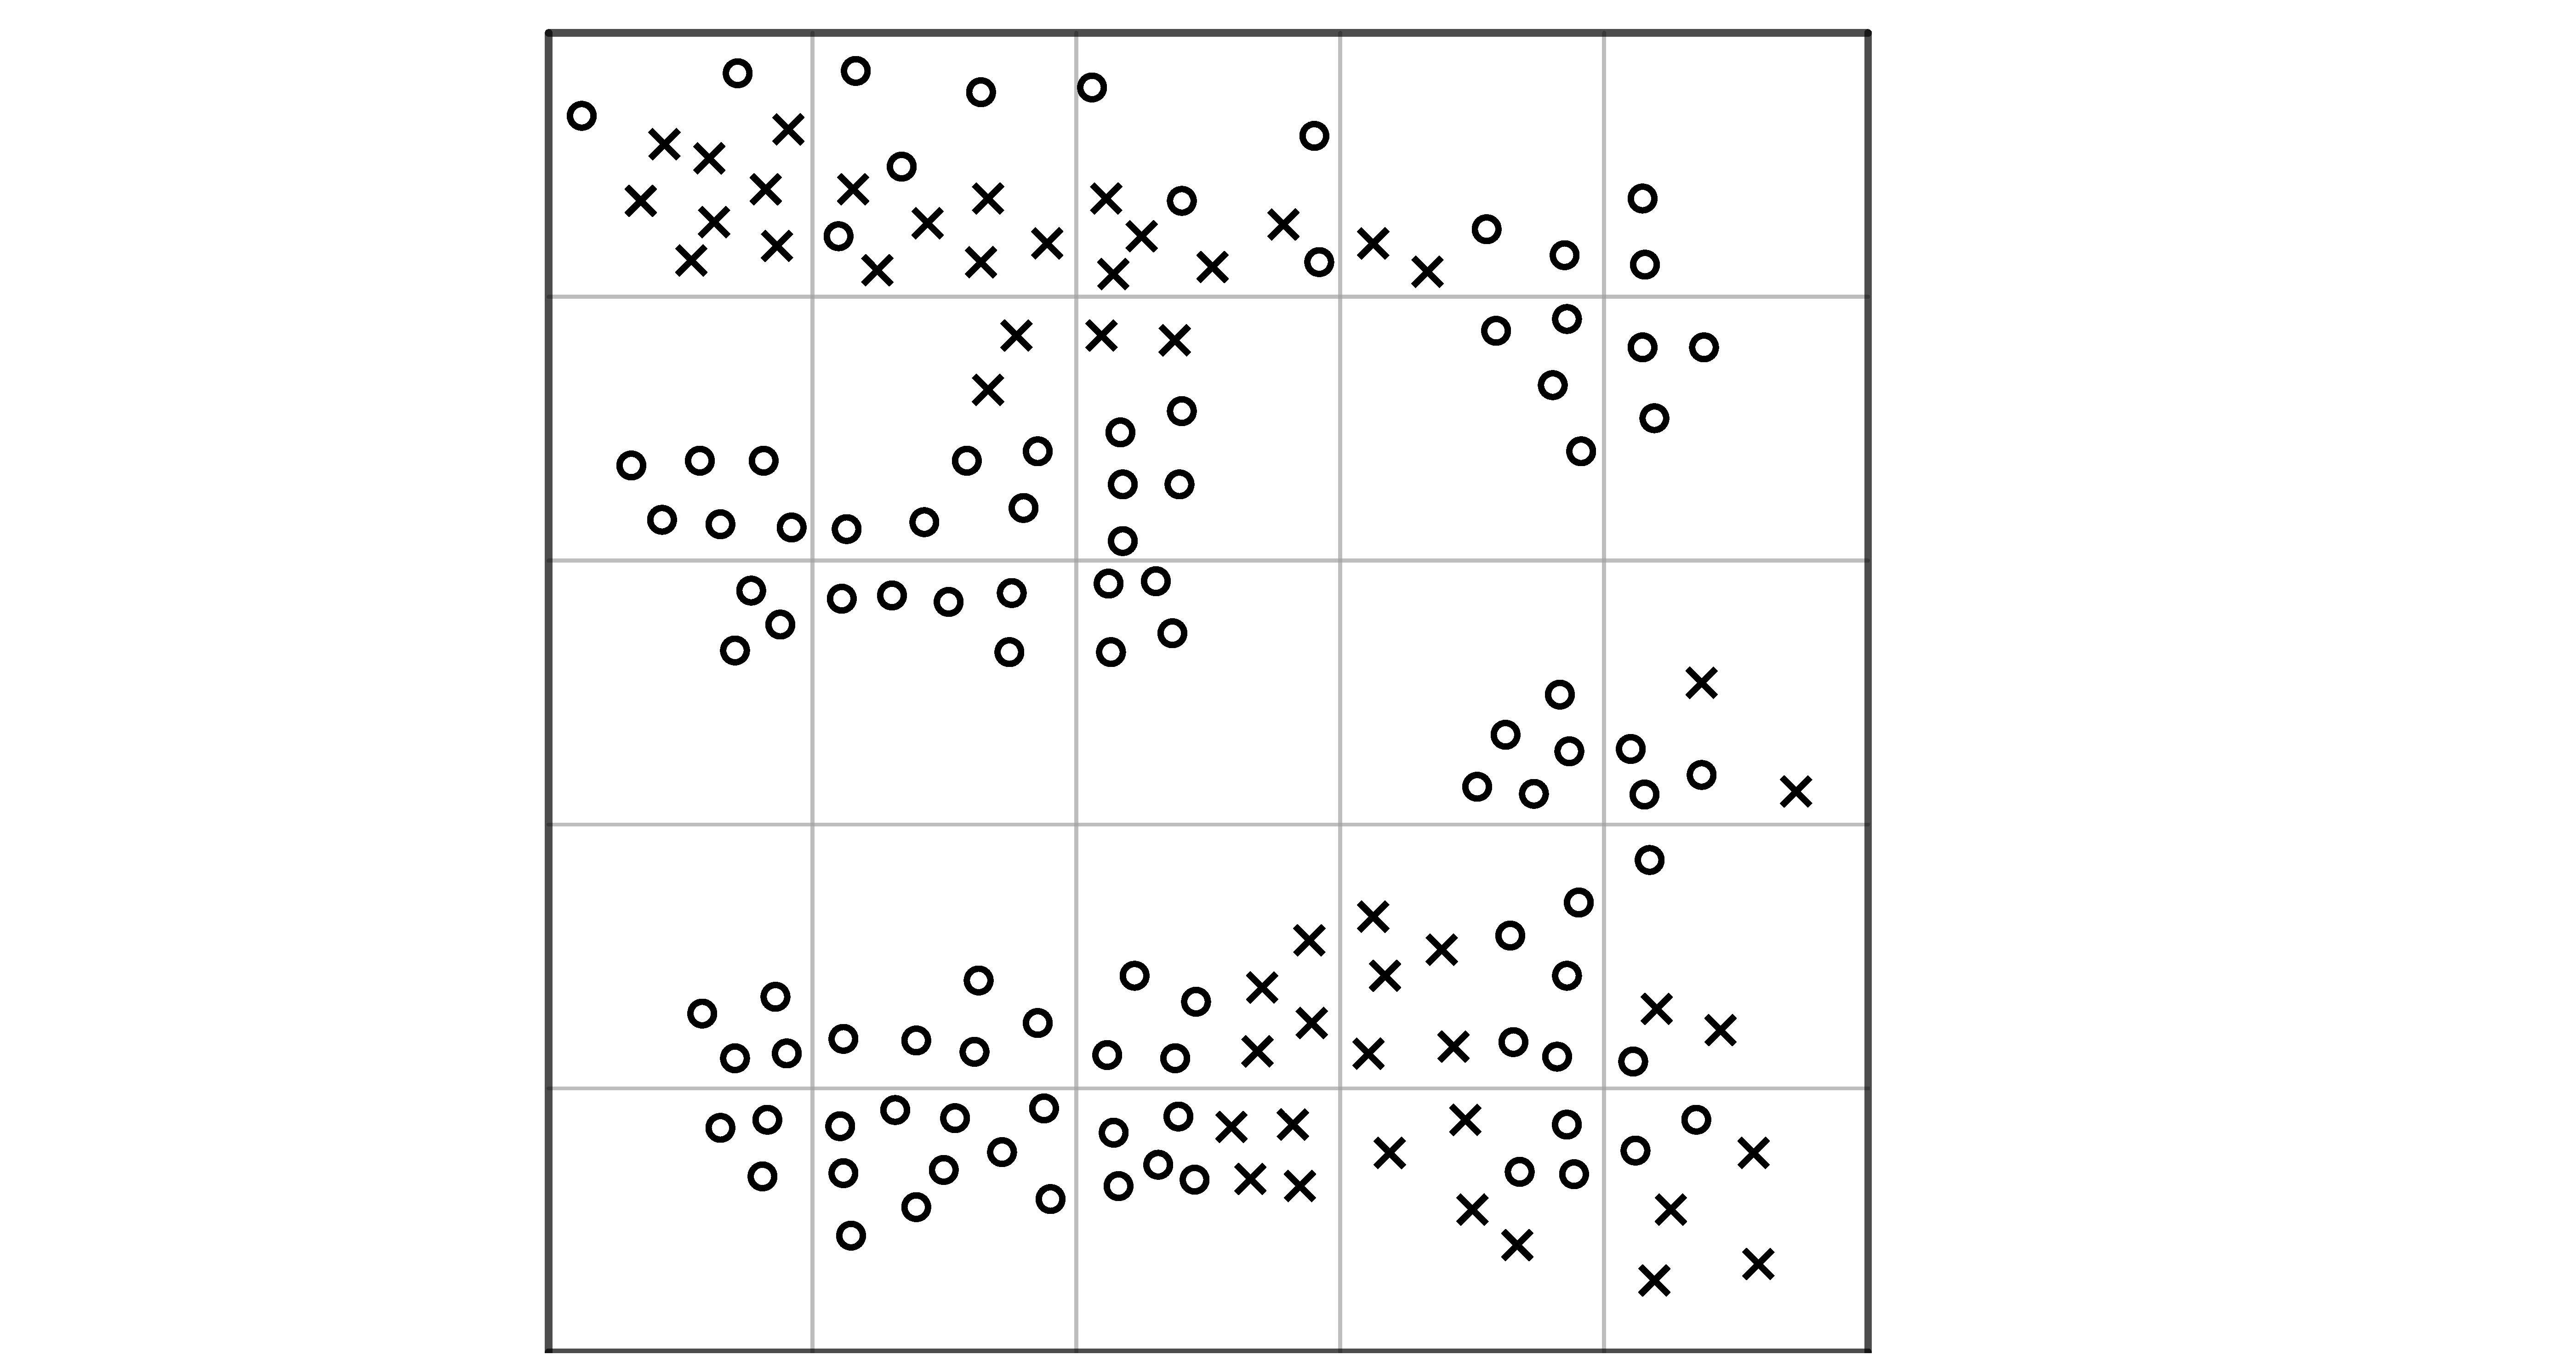
\includegraphics[width=1in]{assets/Gerrymandering/Gerry5x5-150-1.pdf} &  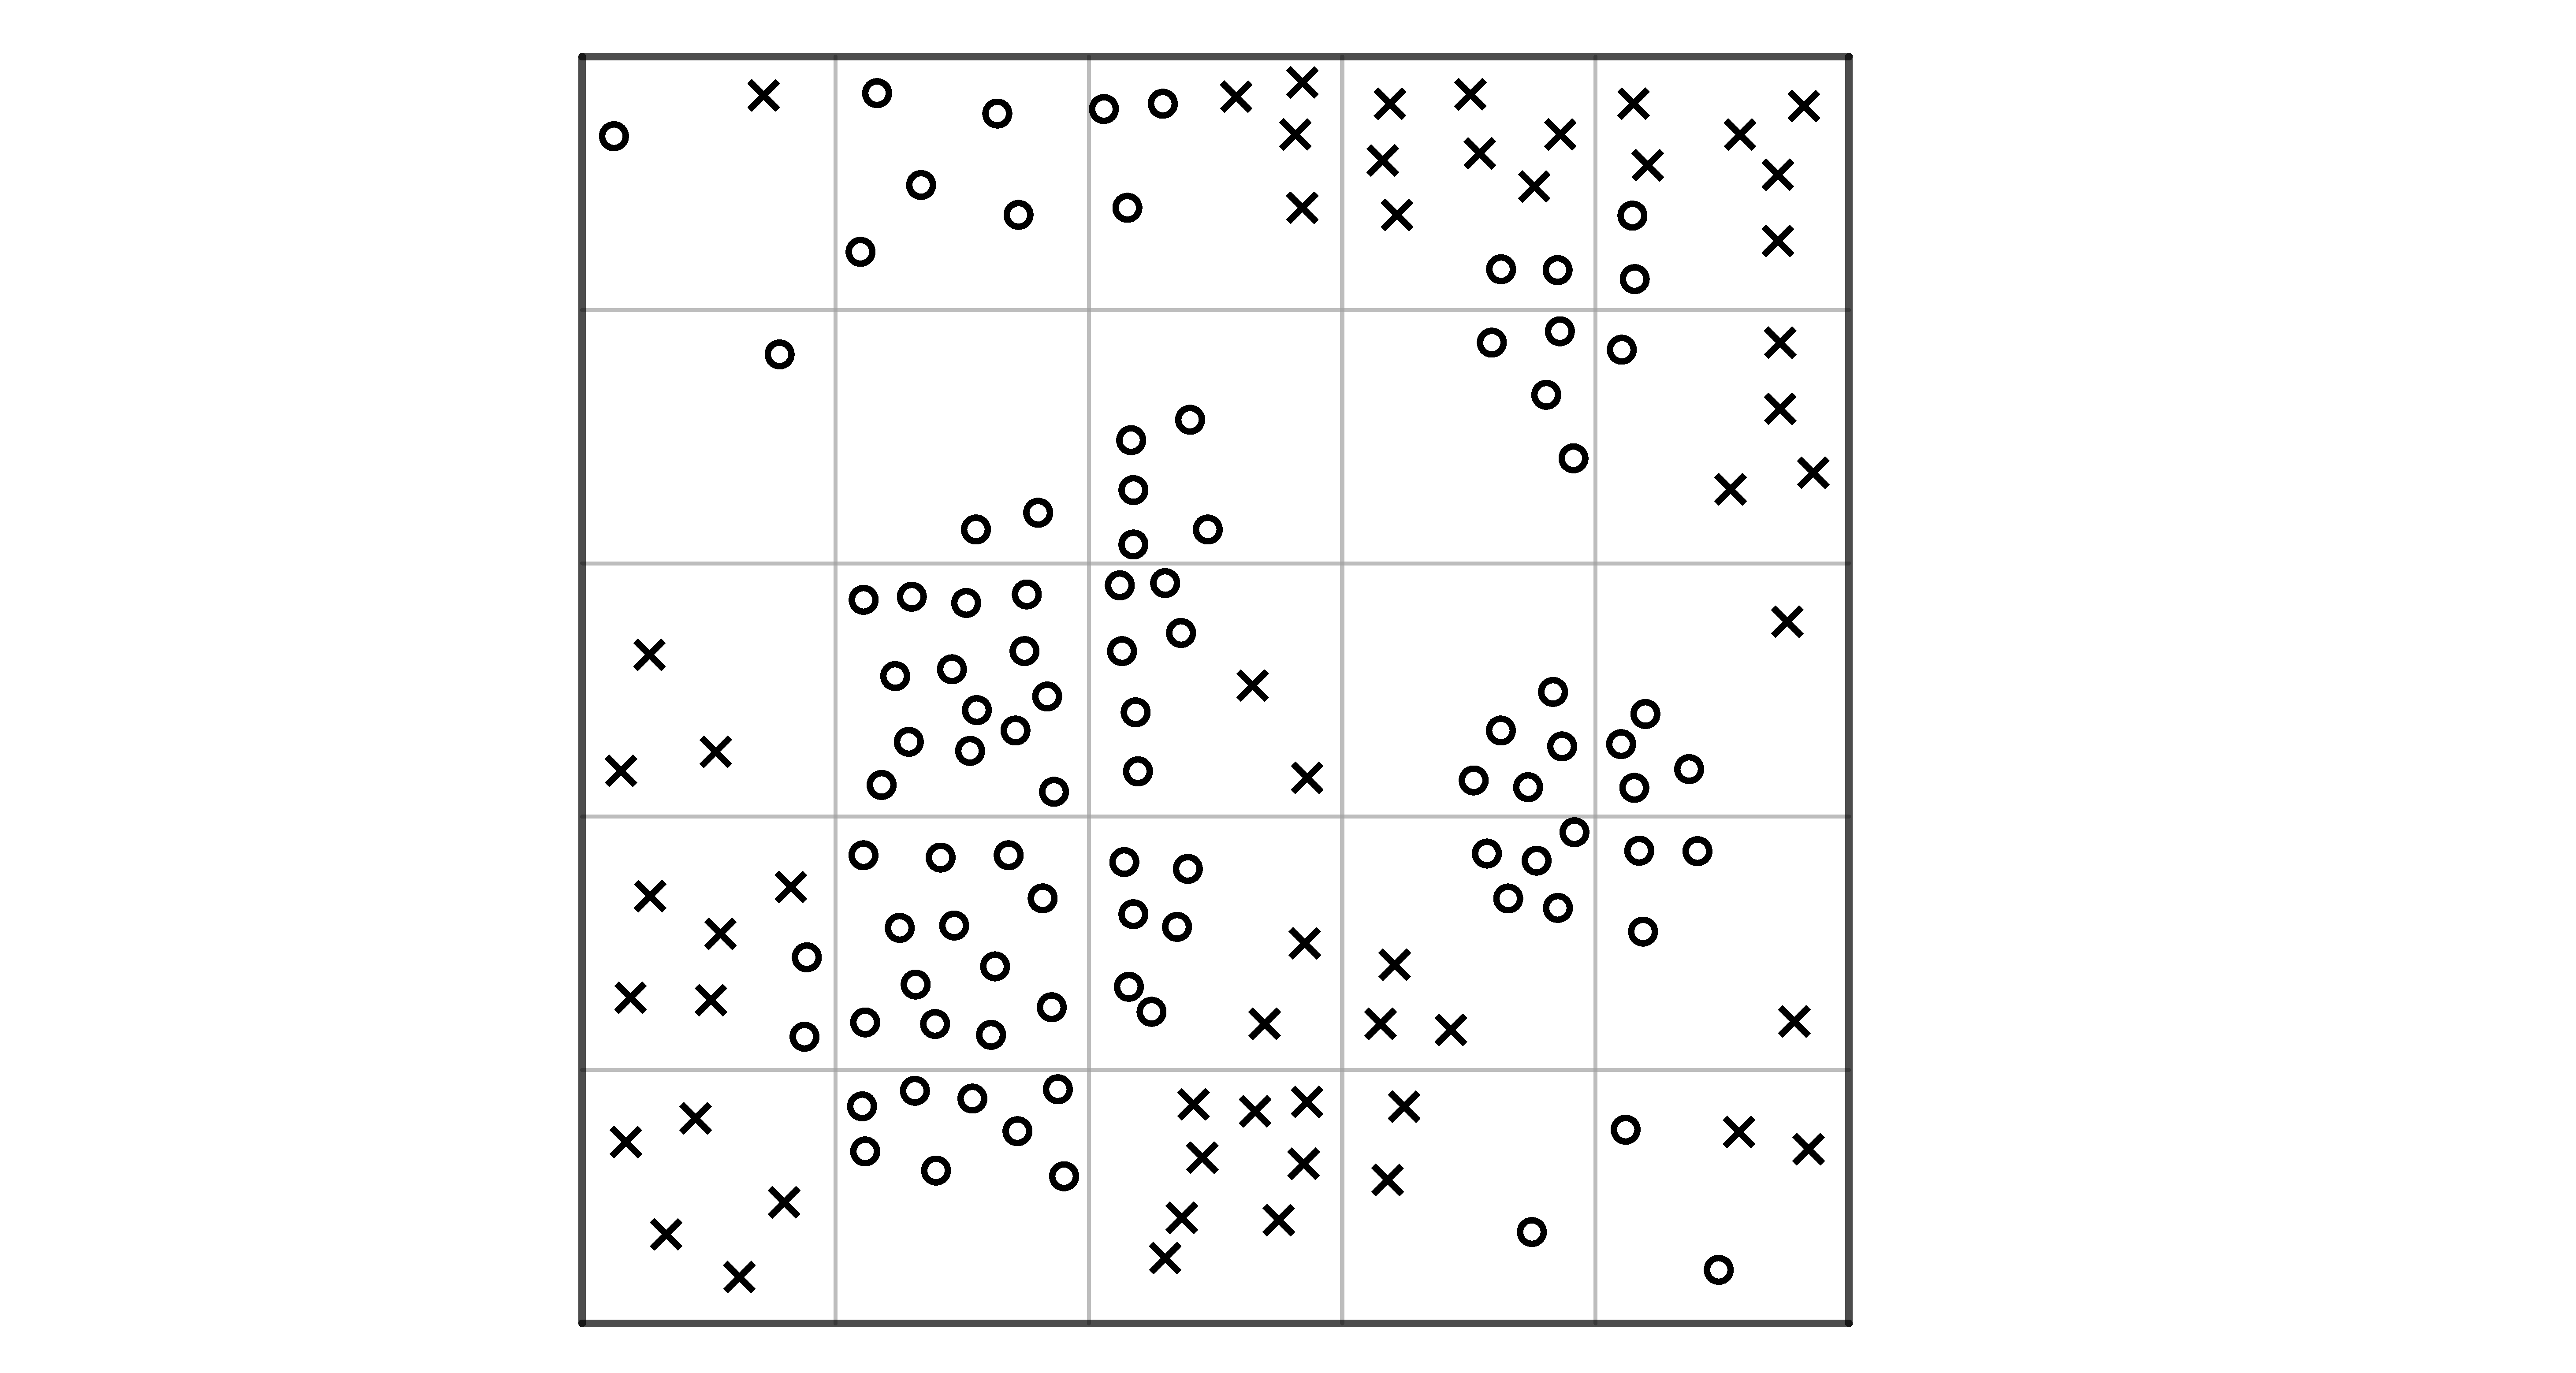
\includegraphics[width=1in]{assets/Gerrymandering/Gerry5x5-150-2.pdf} &  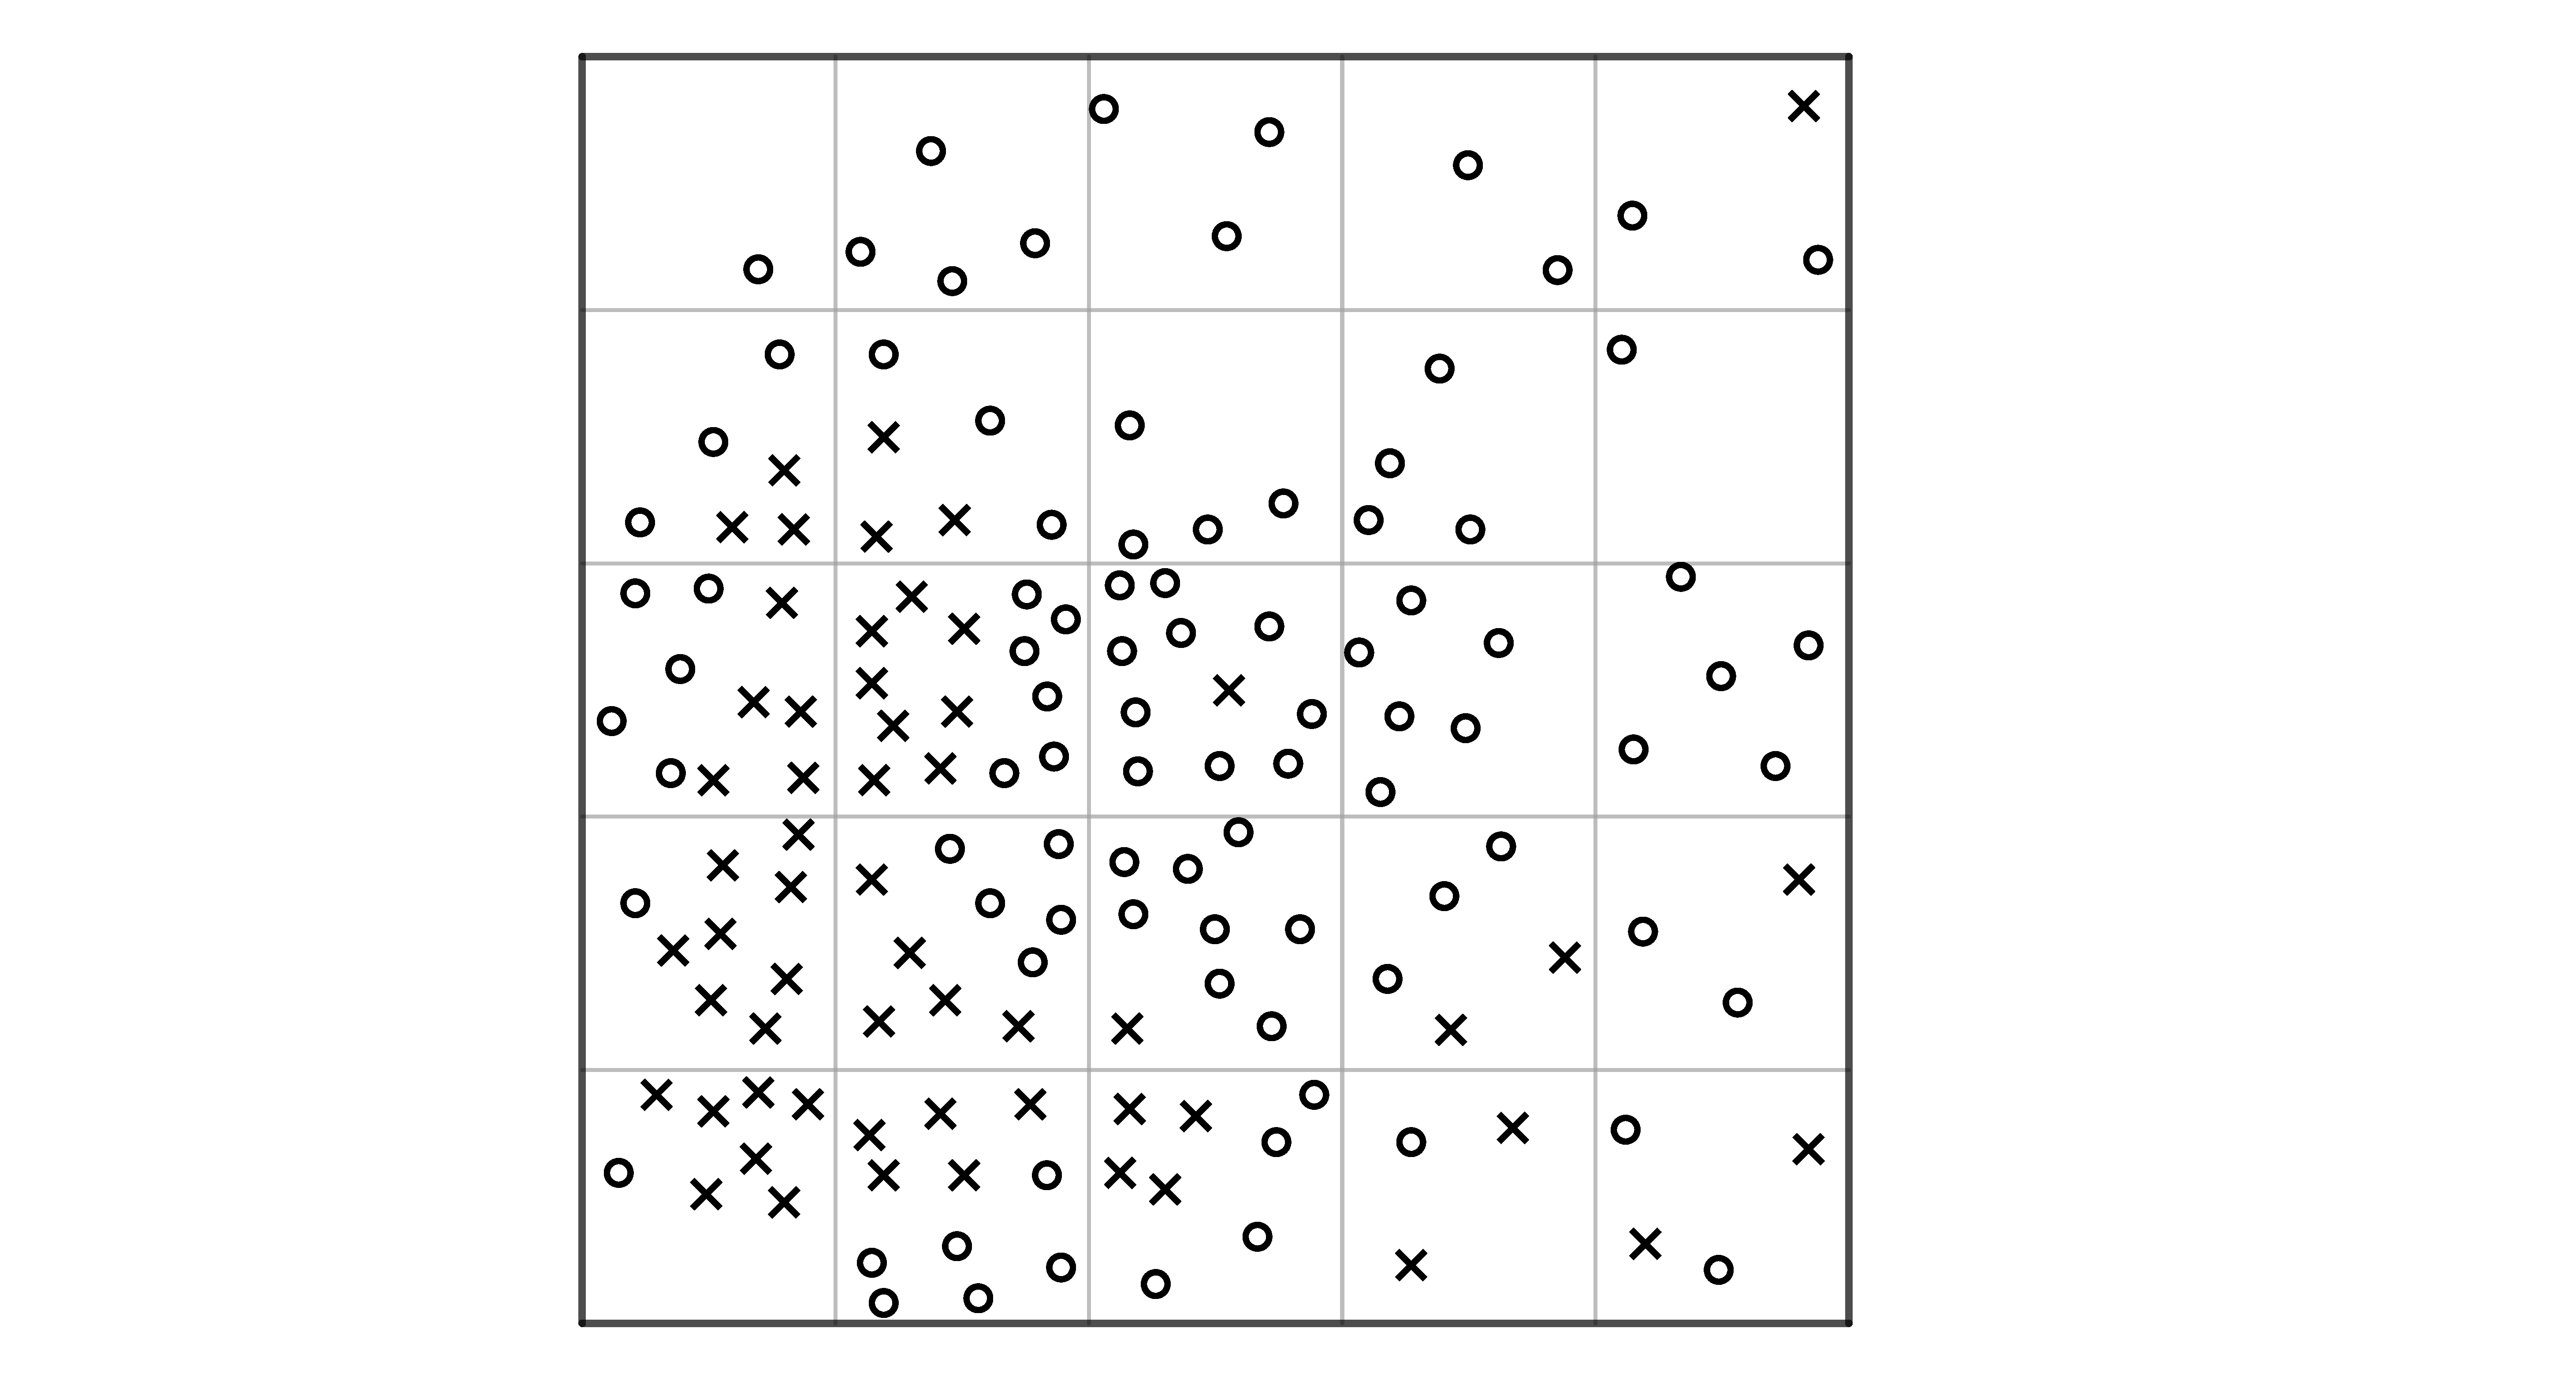
\includegraphics[width=1in]{assets/Gerrymandering/Gerry5x5-150-3.pdf}\\
% Total Vote Count &  Total Vote Count &  Total Vote Count\\
% X -  50& X - 56 & X  - 58\\
% O - 100 & O - 96 & O - 92
% \end{tabular}


\phChapterWorksheet{Tribe C}{Population = 100}

\begin{tabular}{c c c }

Year 1 & Year 2 & Year 3 \\
 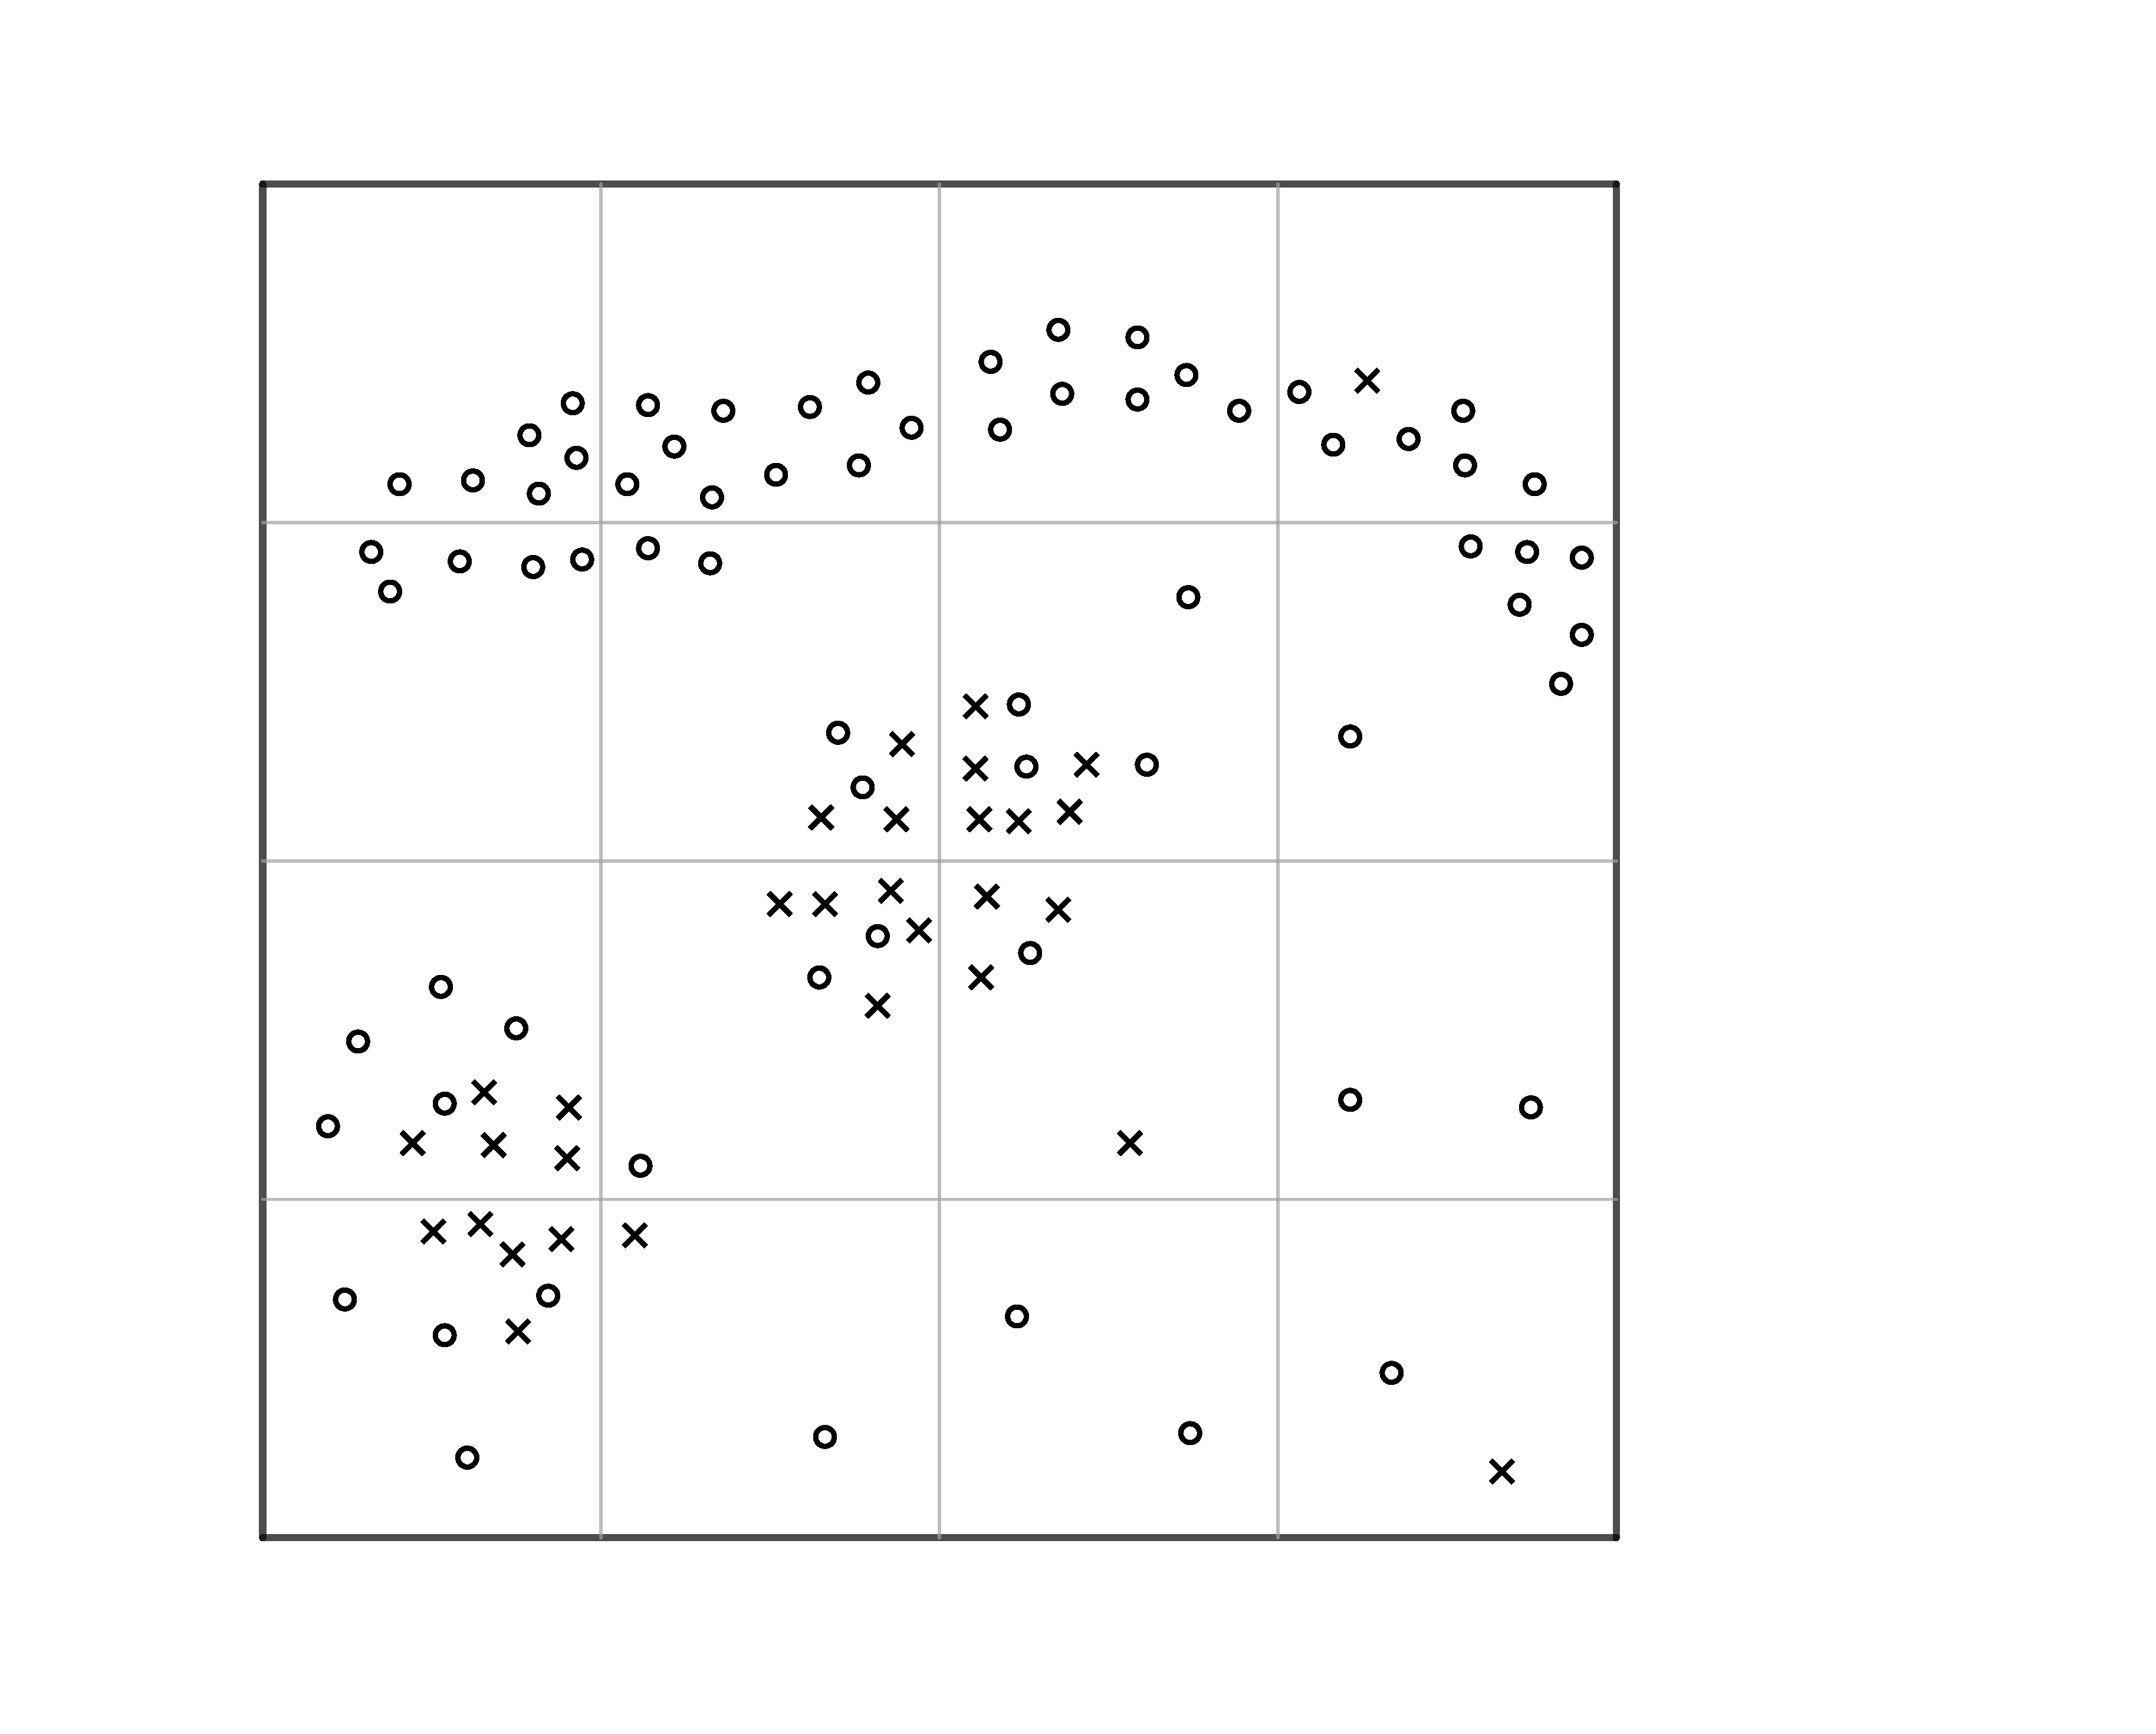
\includegraphics[width=2in]{assets/Gerrymandering/Gerry4x4-100-1.pdf} &  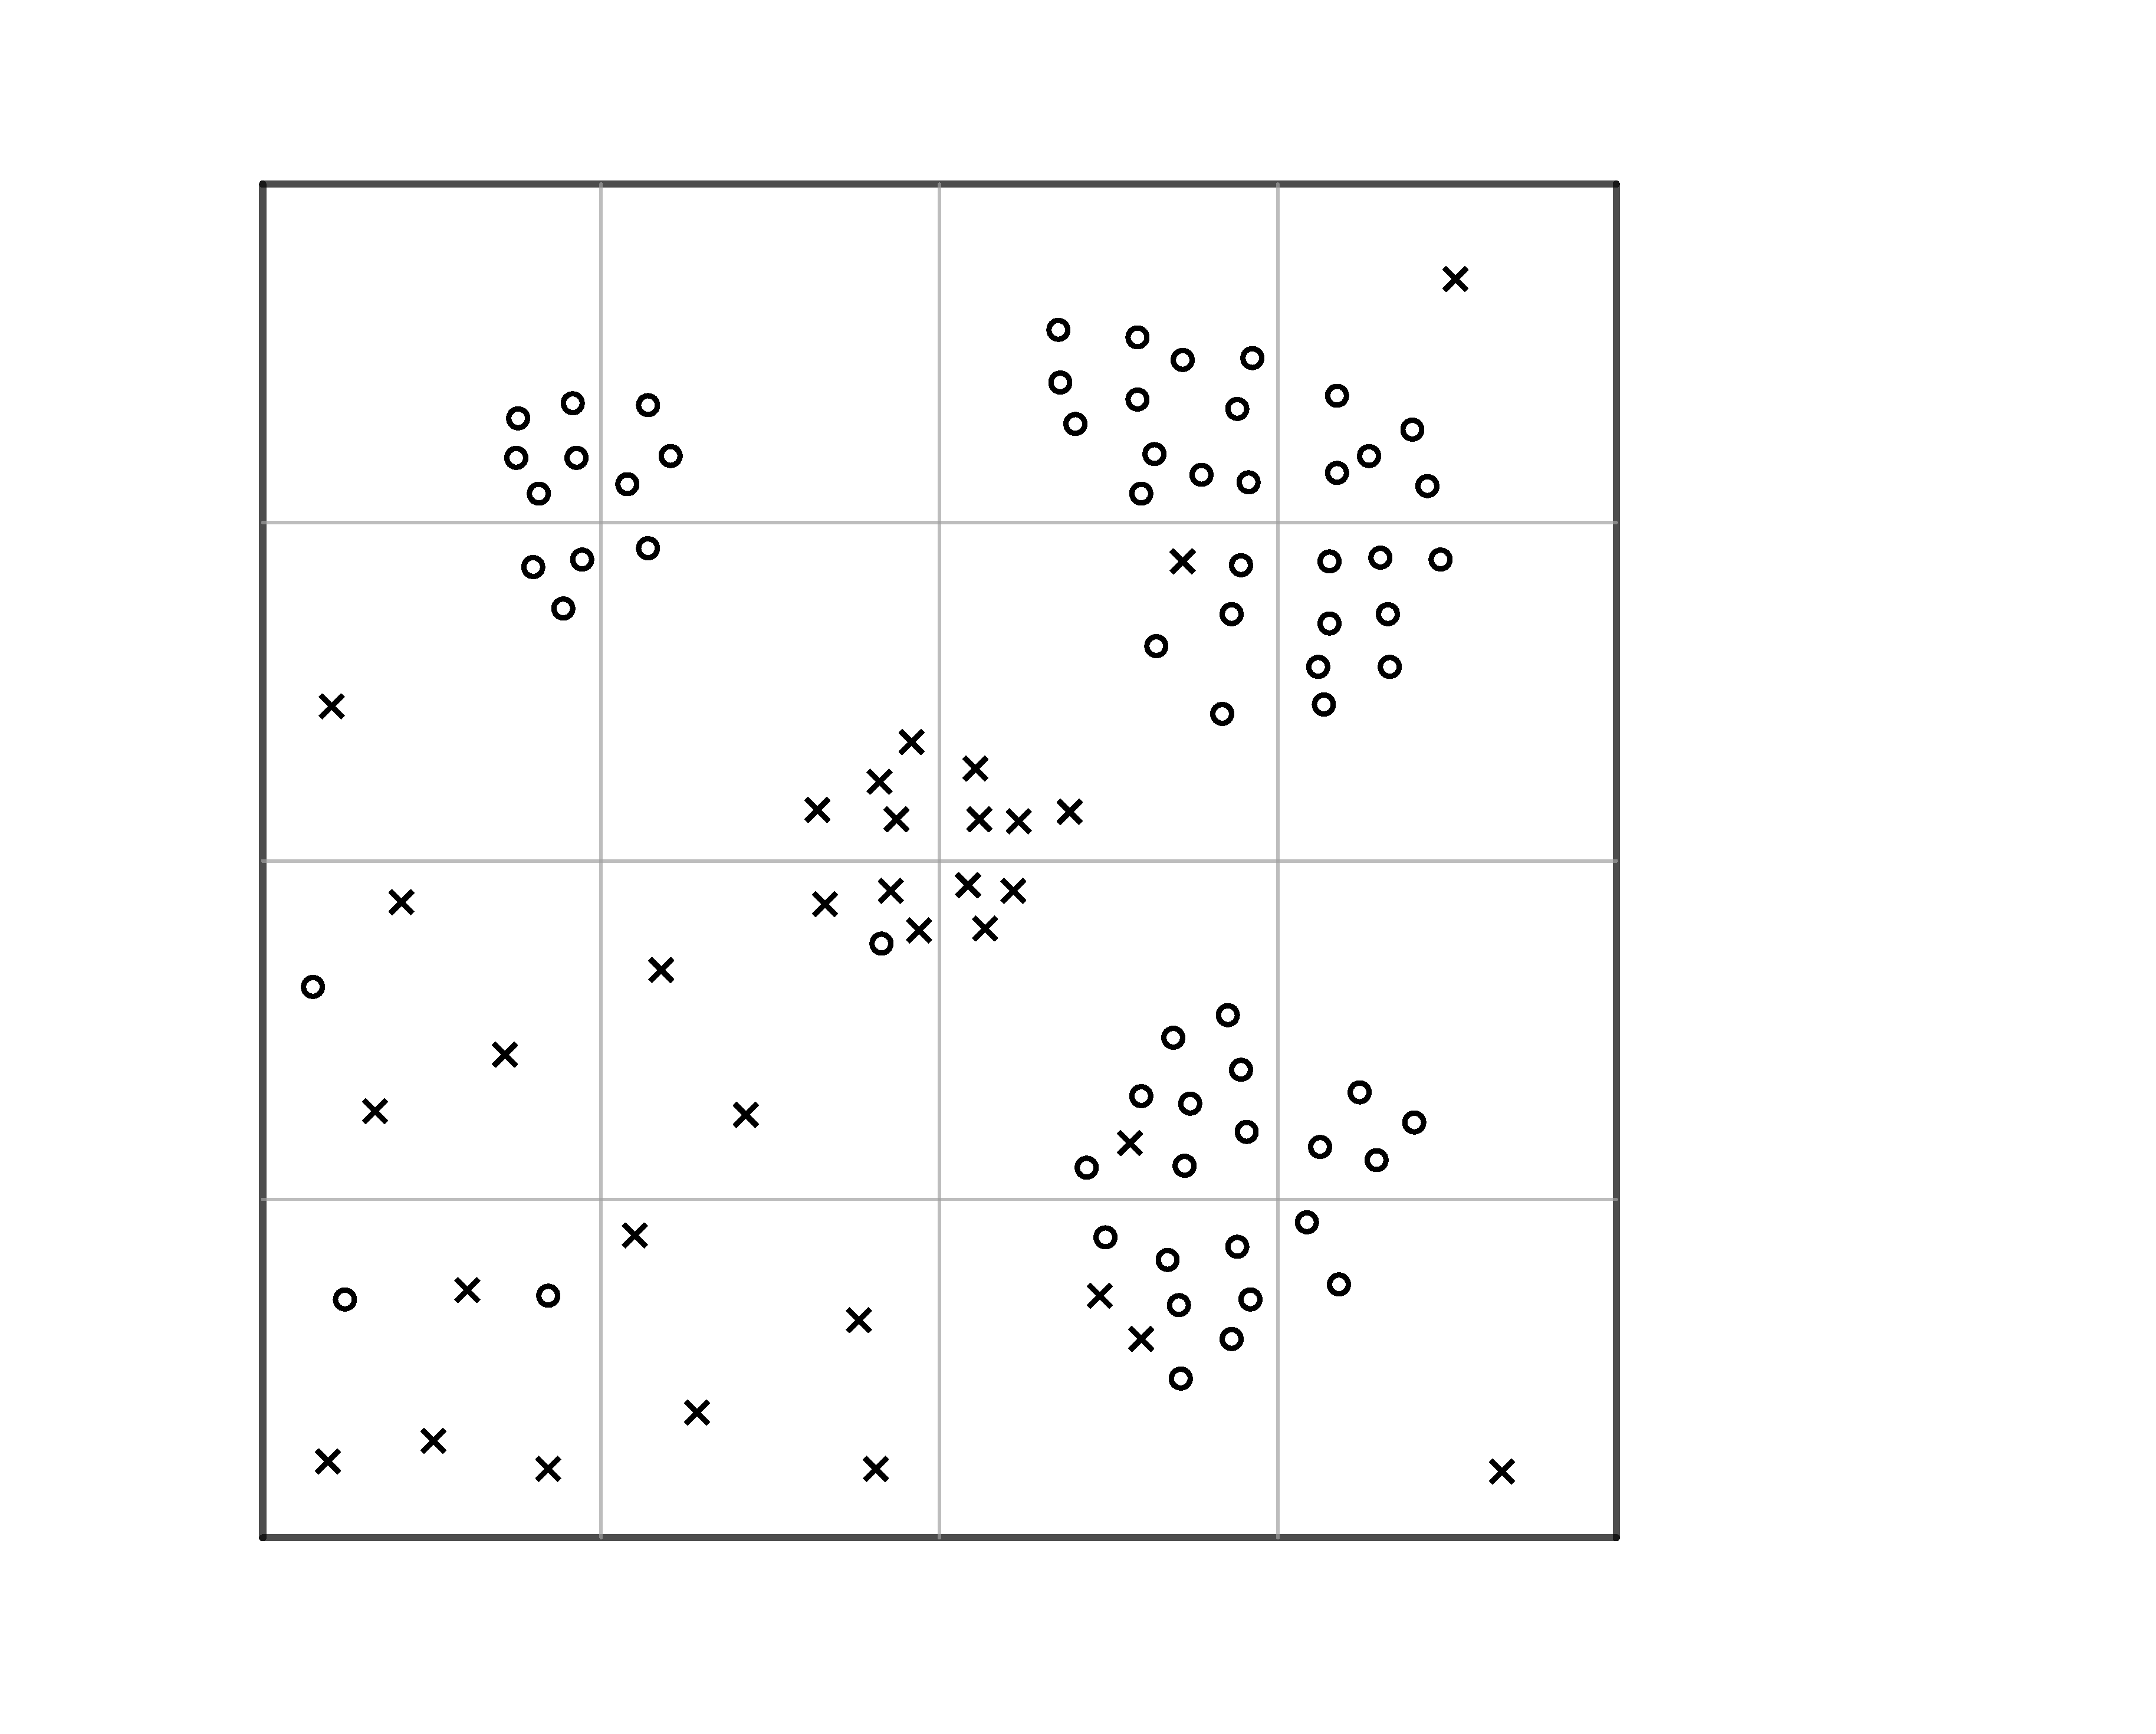
\includegraphics[width=2in]{assets/Gerrymandering/Gerry4x4-100-2.pdf} &  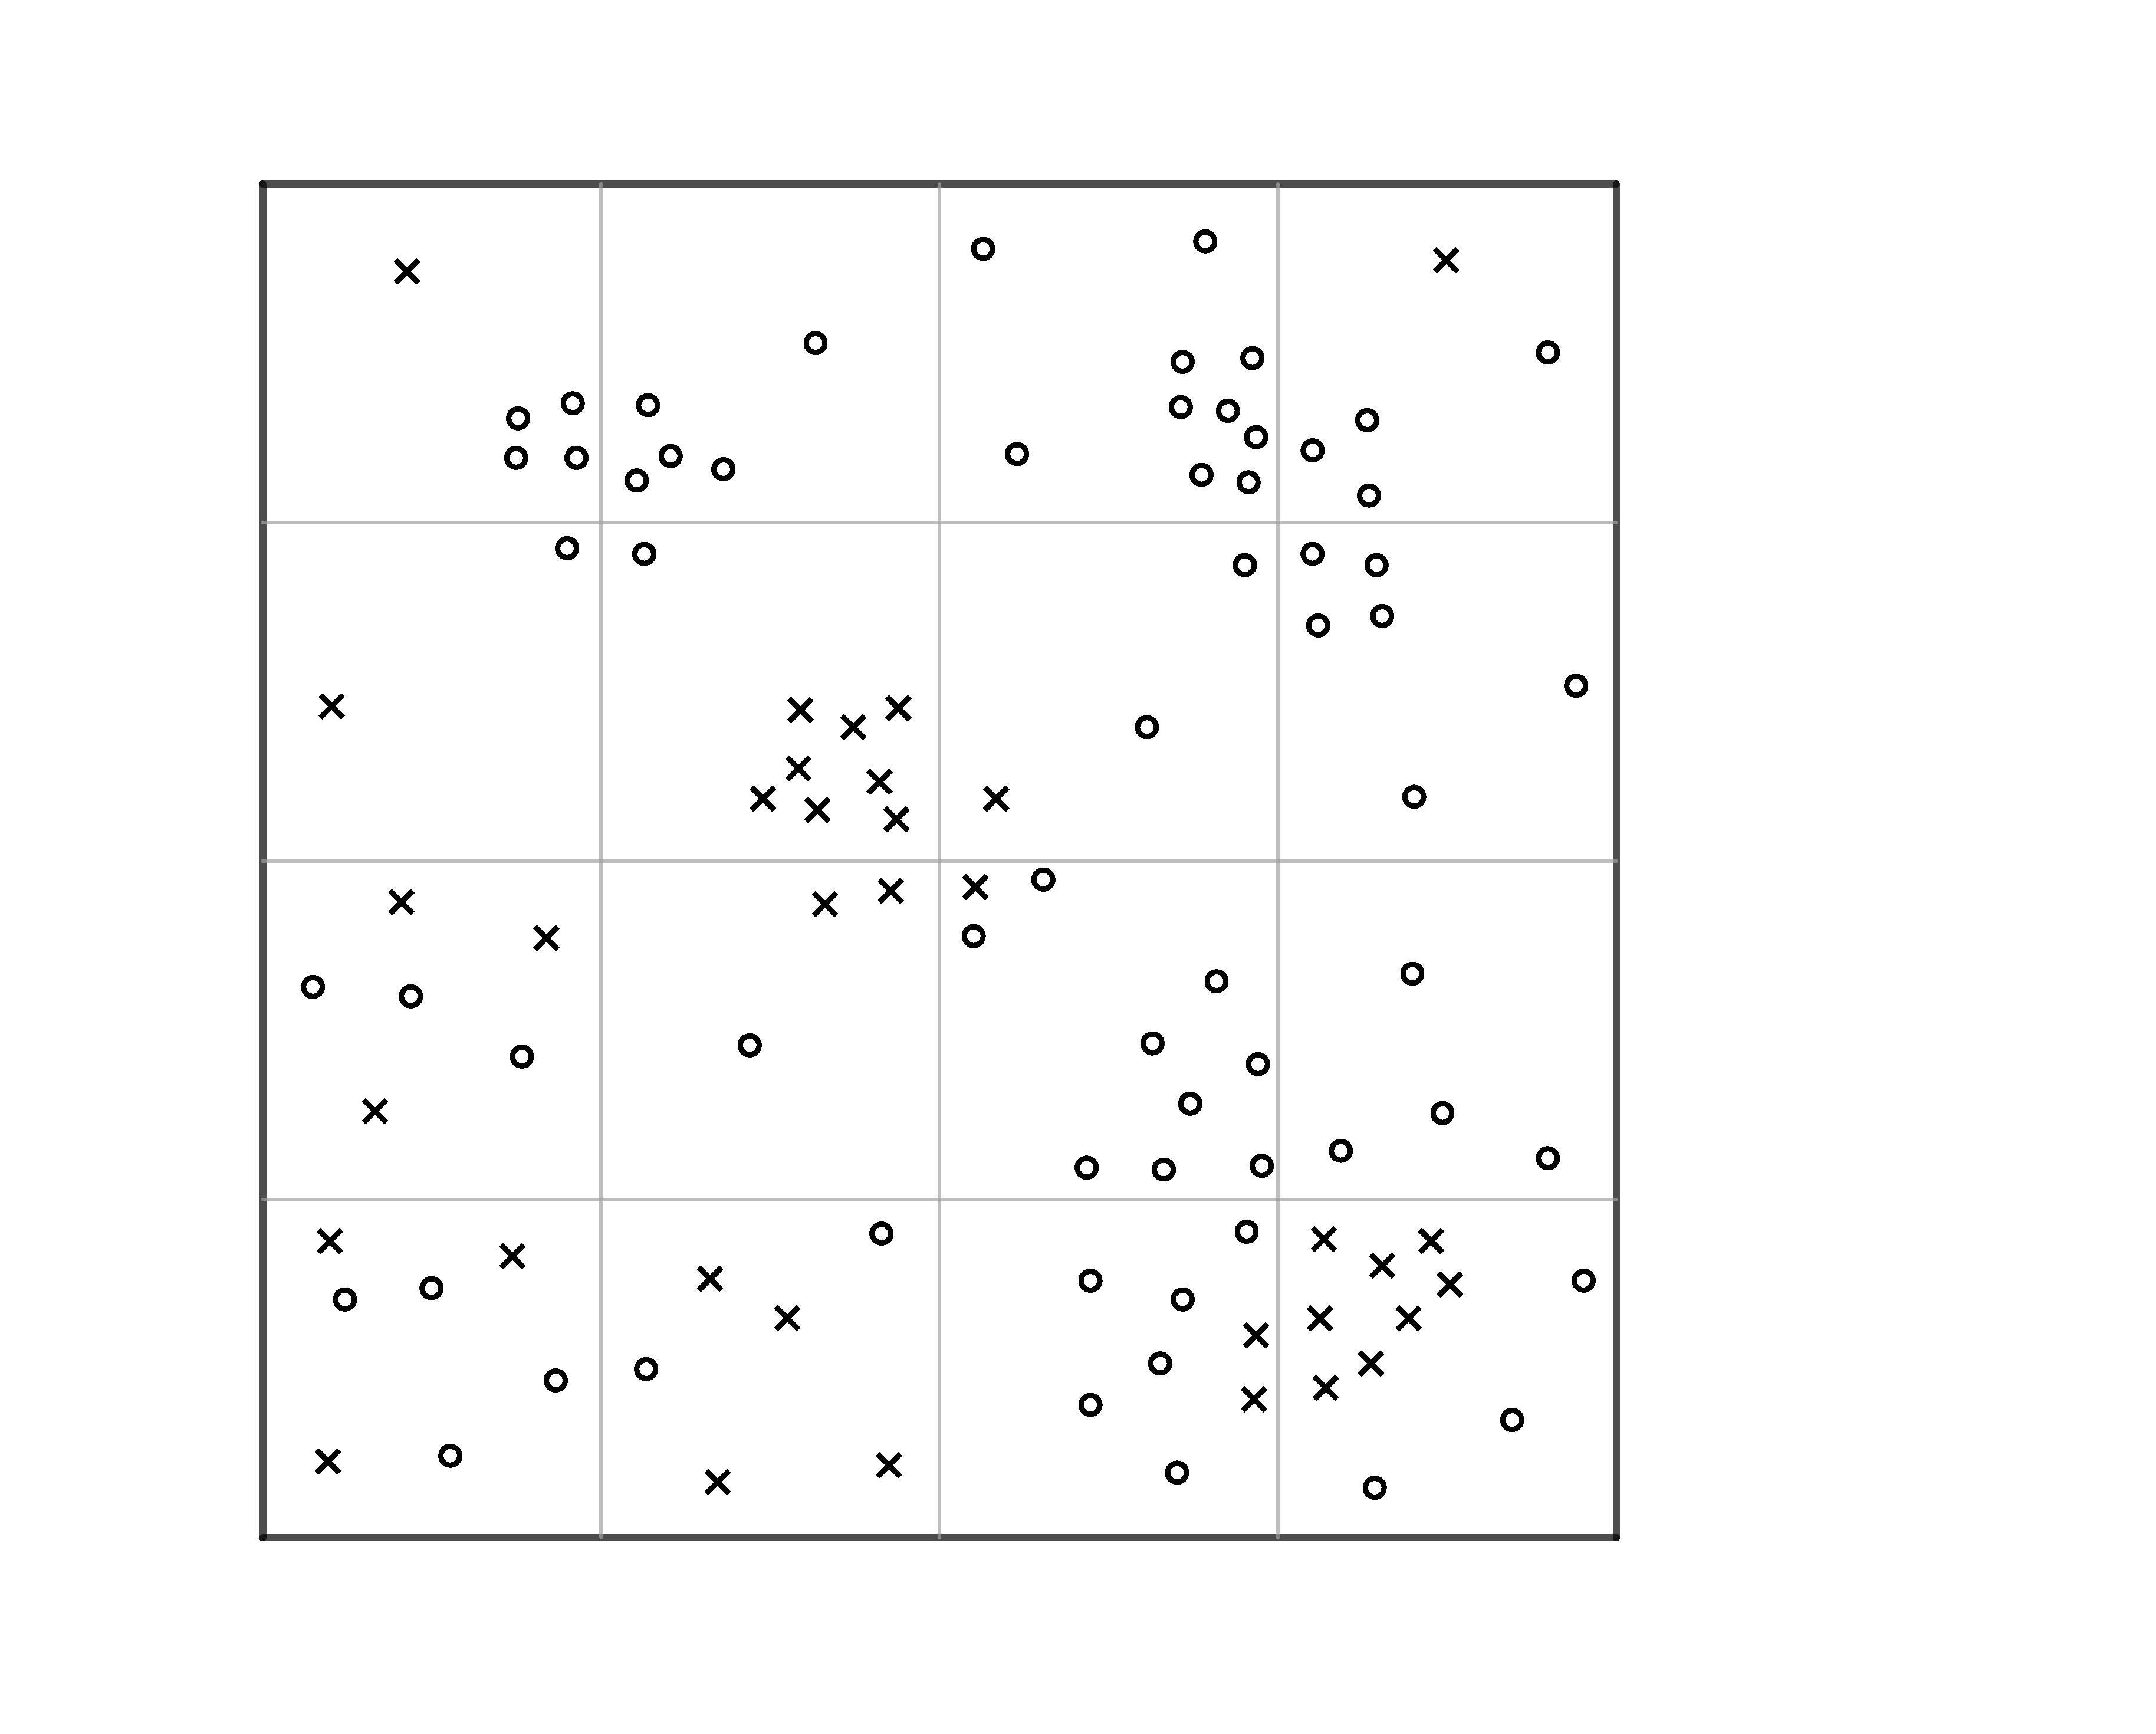
\includegraphics[width=2in]{assets/Gerrymandering/Gerry4x4-100-3.pdf}\\
 Total Vote Count &  Total Vote Count &  Total Vote Count\\
 X -  31& X - 34 & X  - 35\\
 O - 69 & O - 66 & O - 65
 \end{tabular}

\phChapterWorksheet{Tribe D}{Population = 100}

\begin{tabular}{c c c }

Year 1 & Year 2 & Year 3 \\
 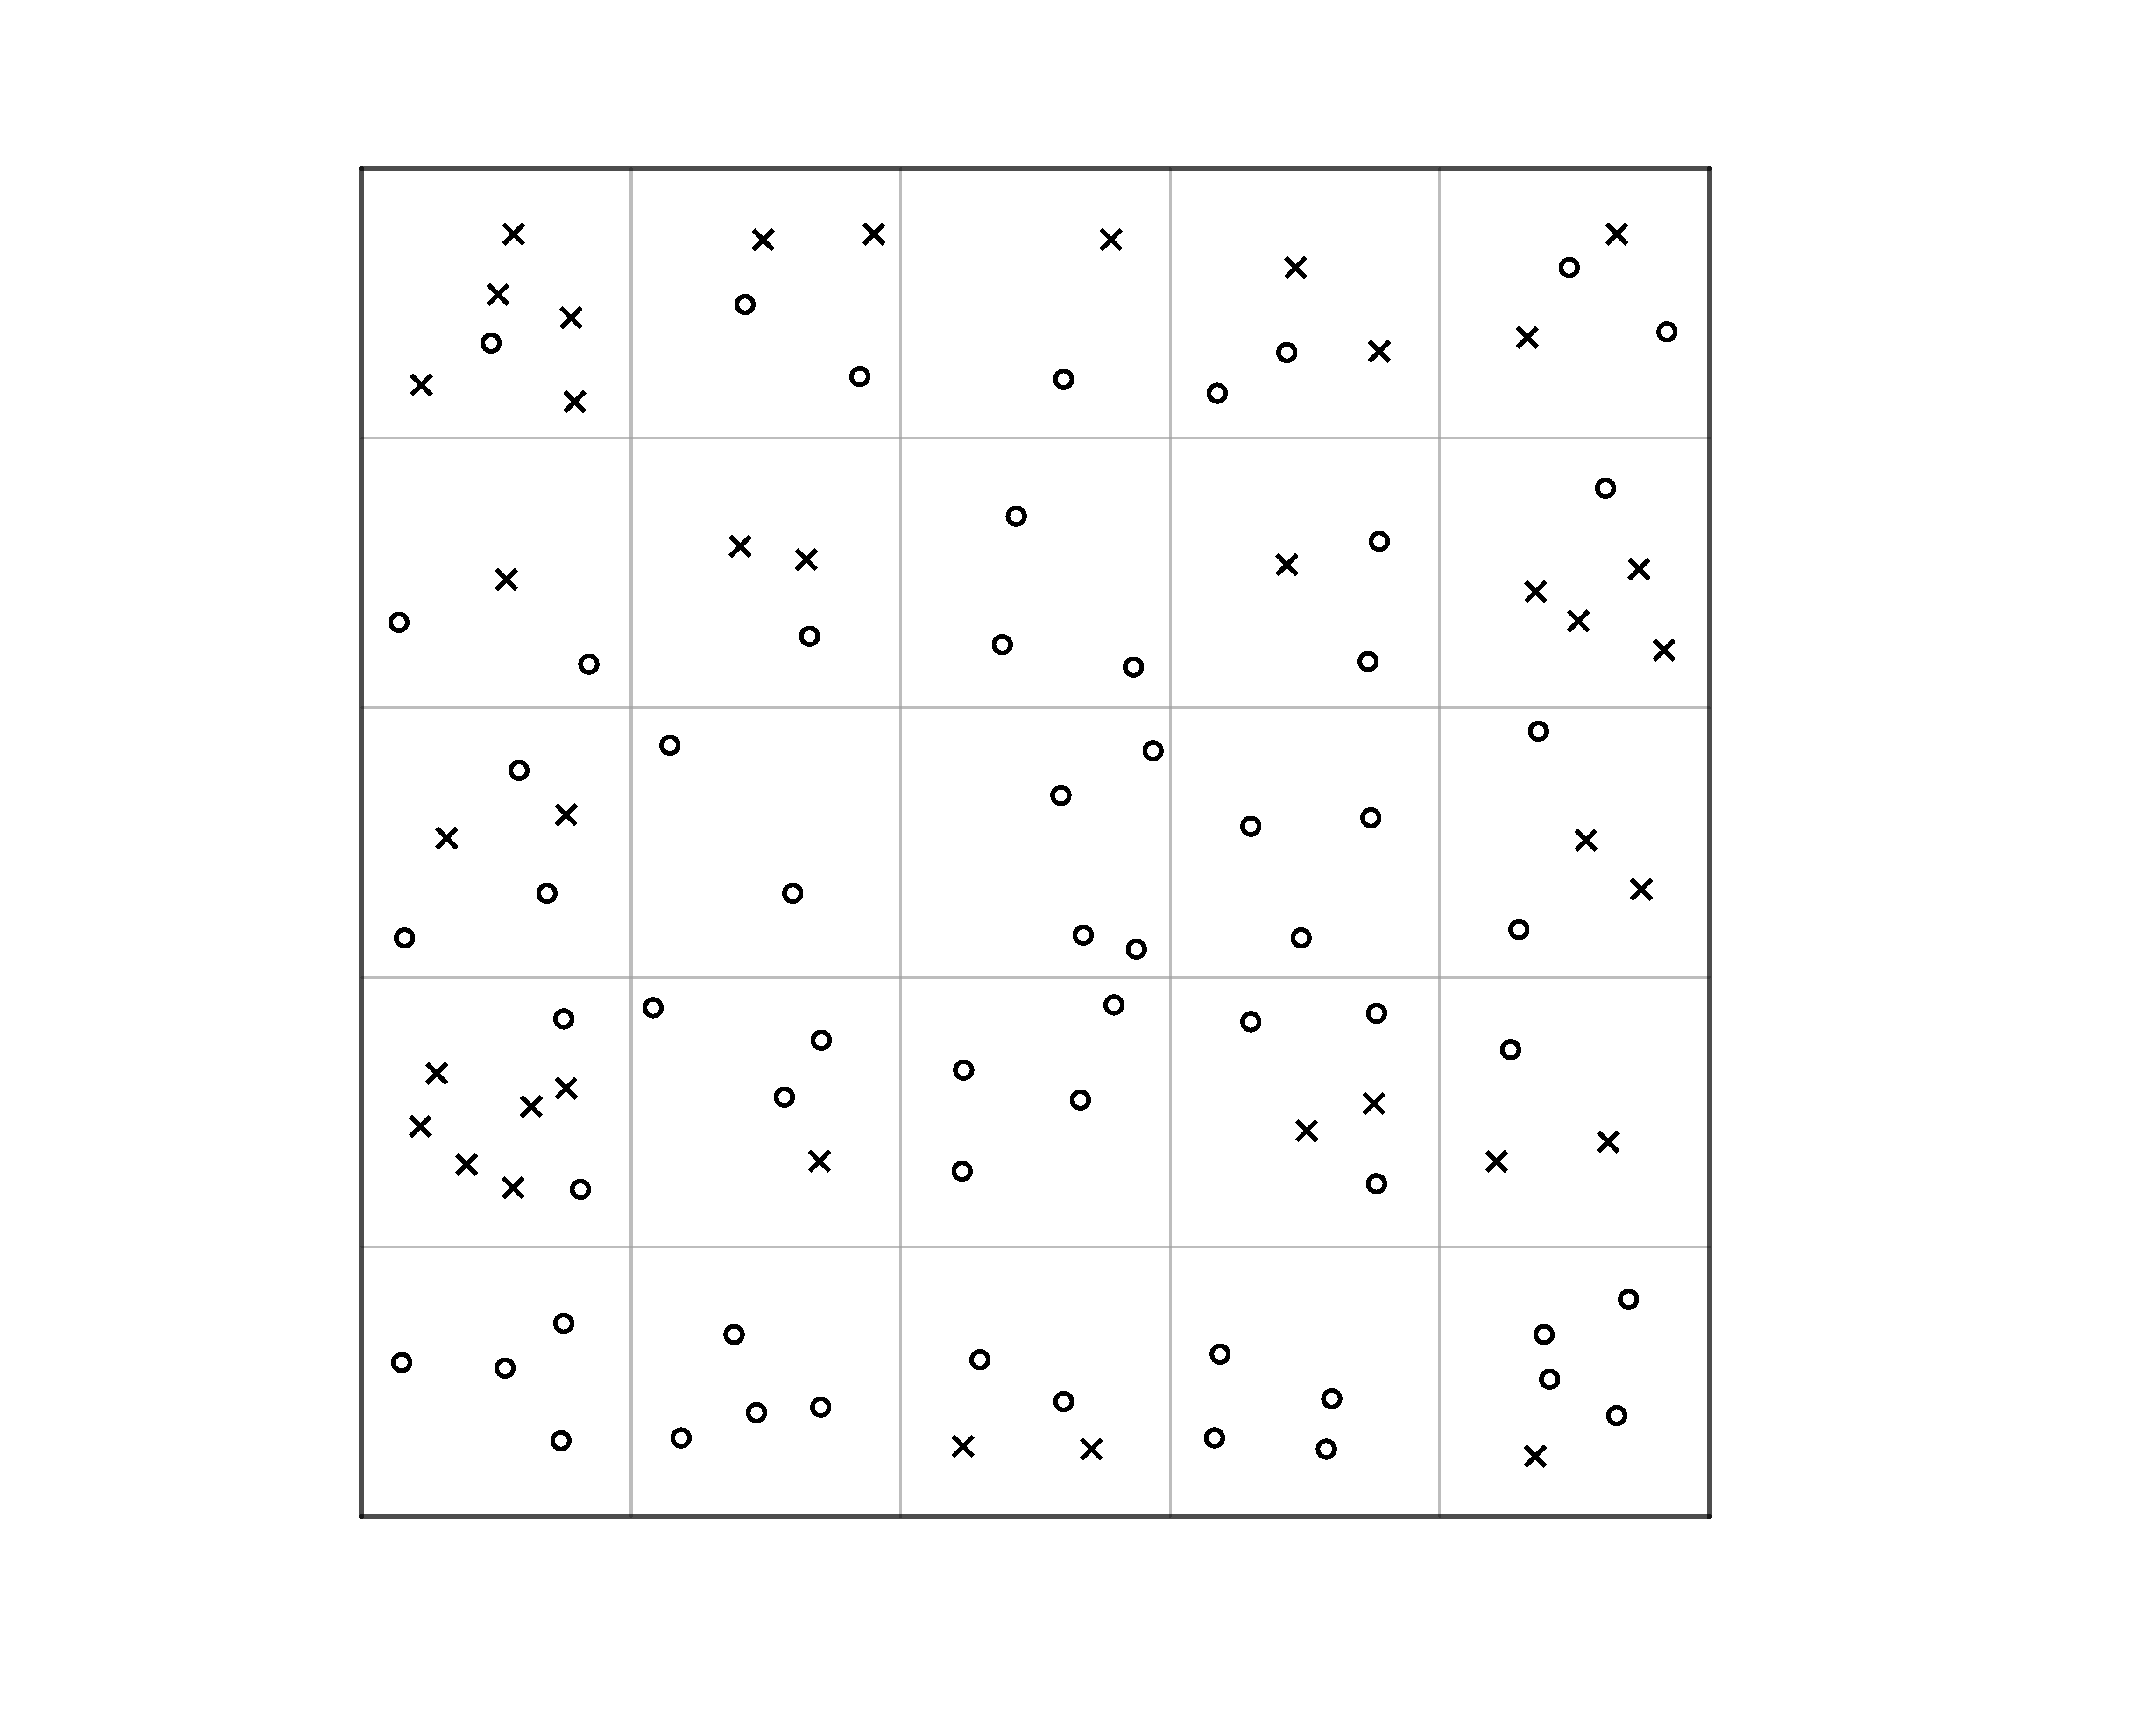
\includegraphics[width=2in]{assets/Gerrymandering/Gerry5x5-100-1.pdf} &  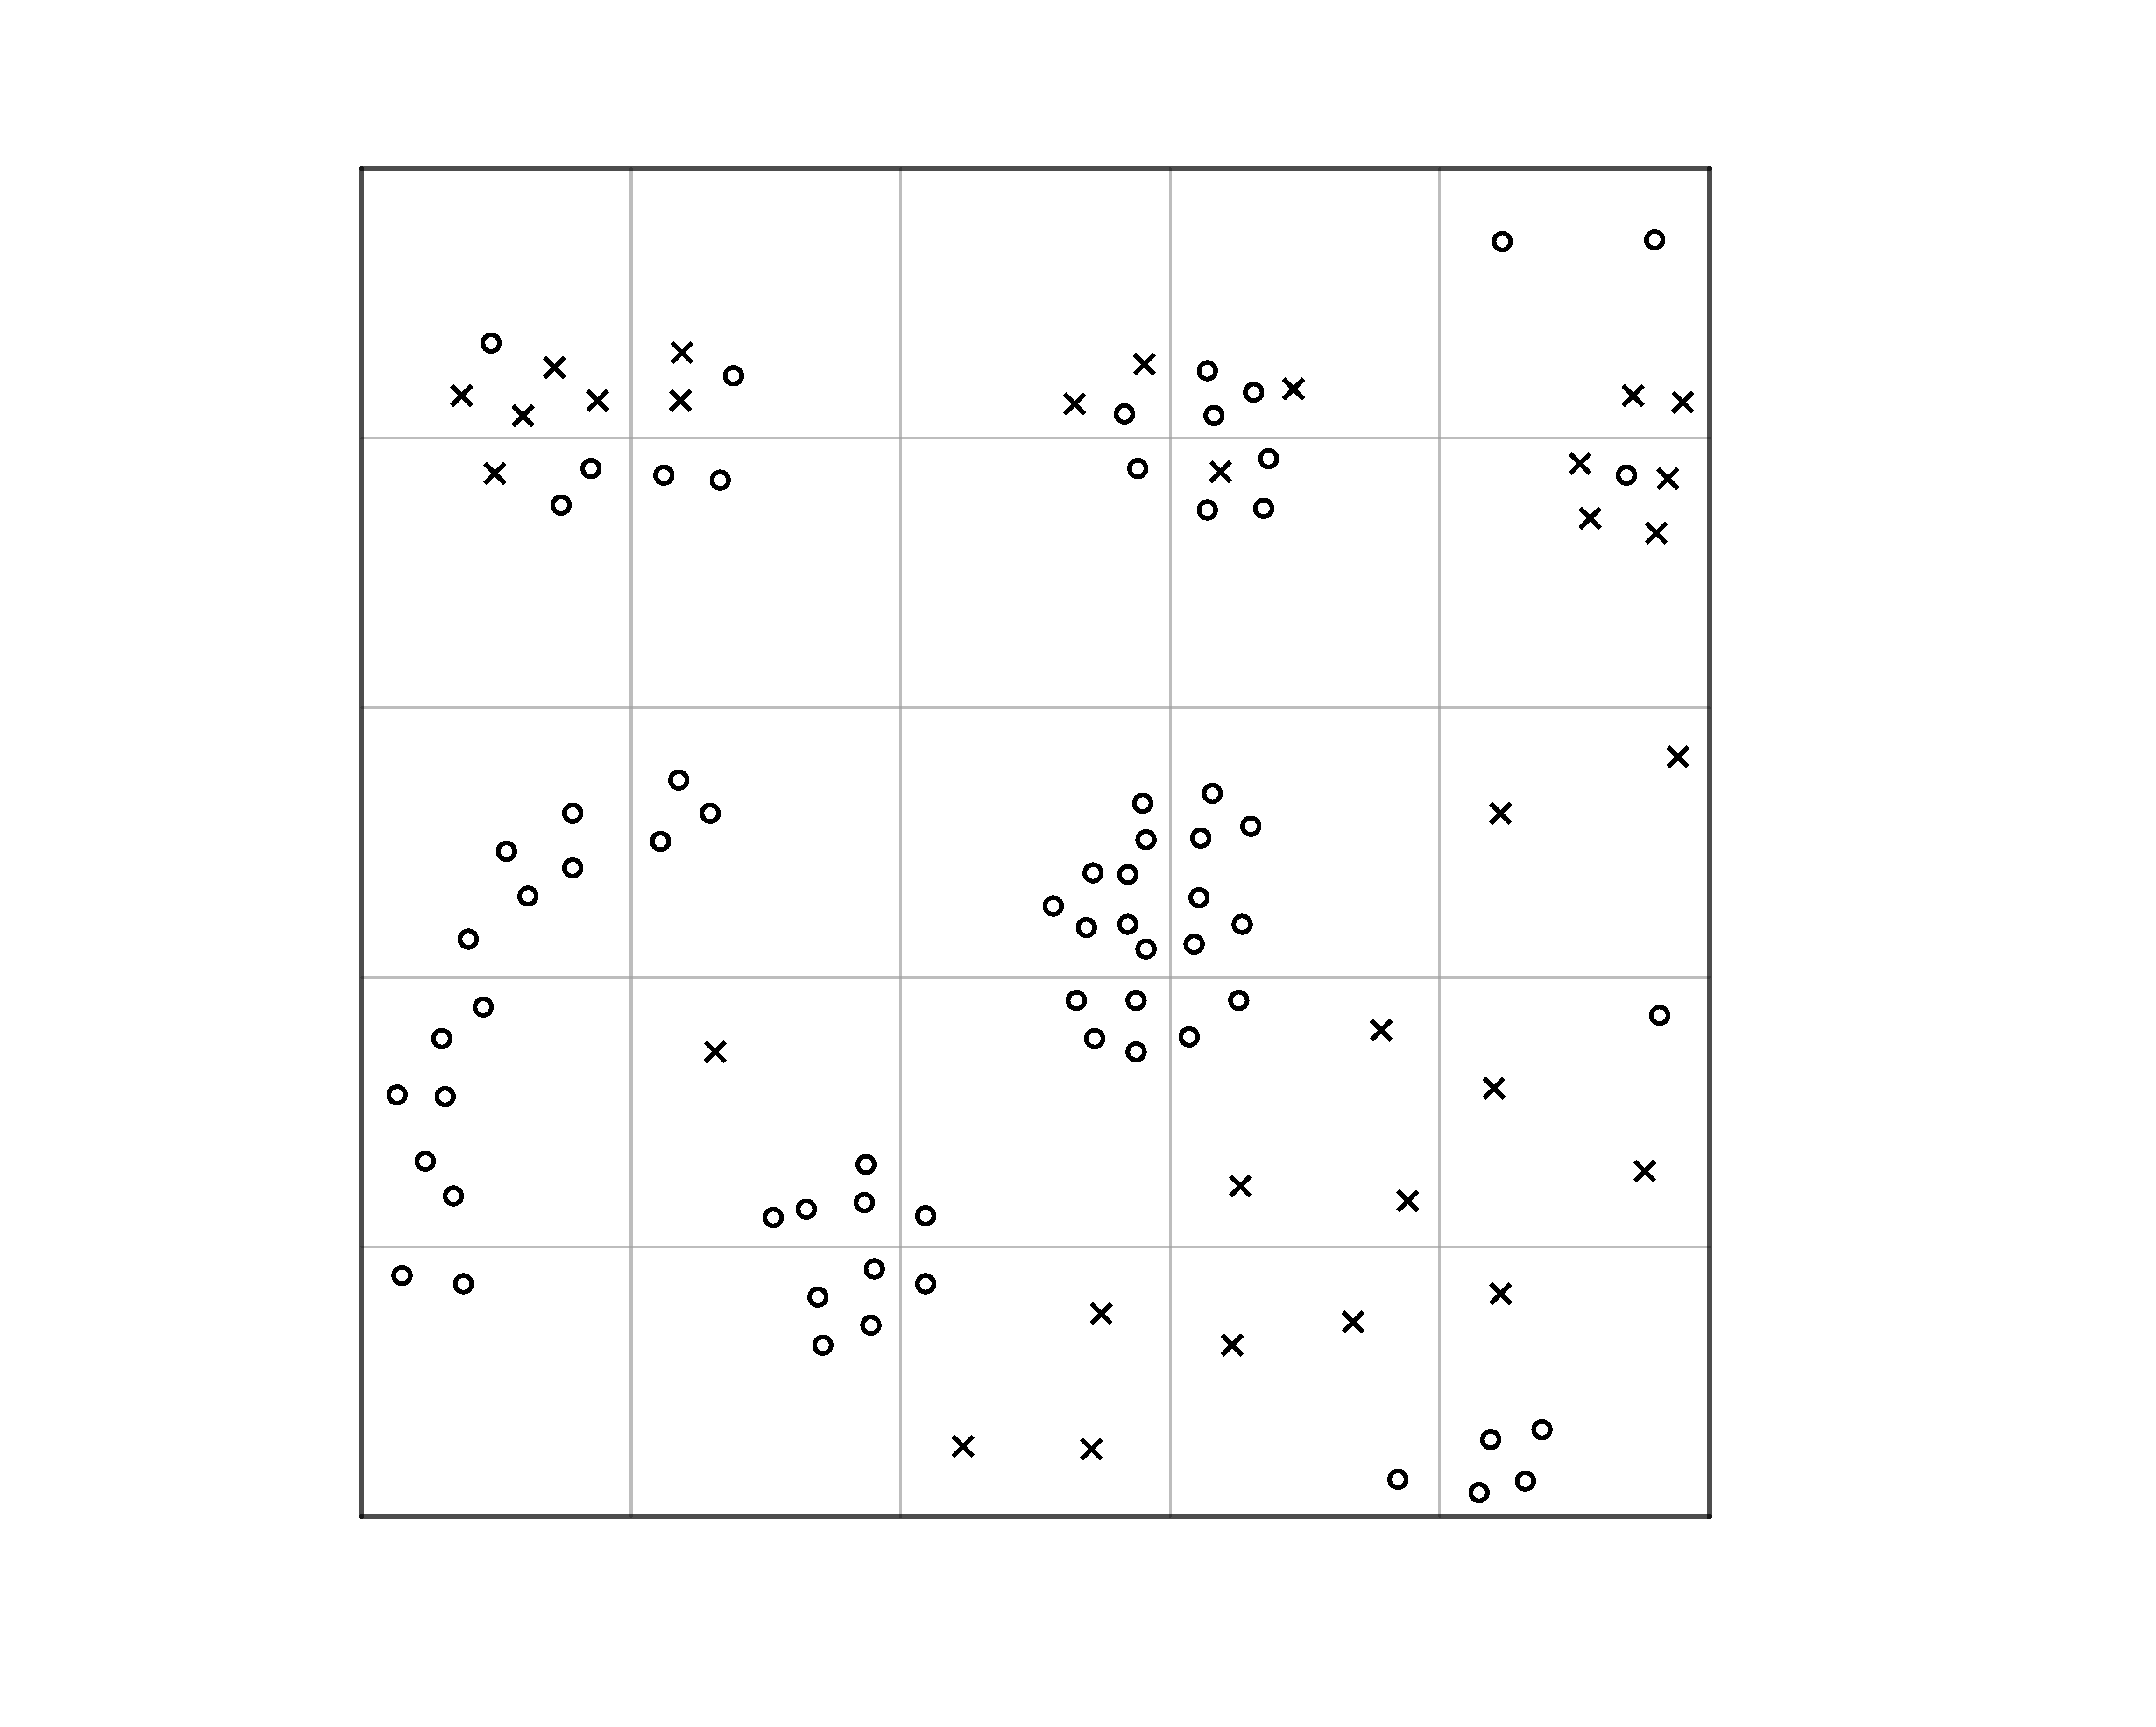
\includegraphics[width=2in]{assets/Gerrymandering/Gerry5x5-100-2.pdf} &  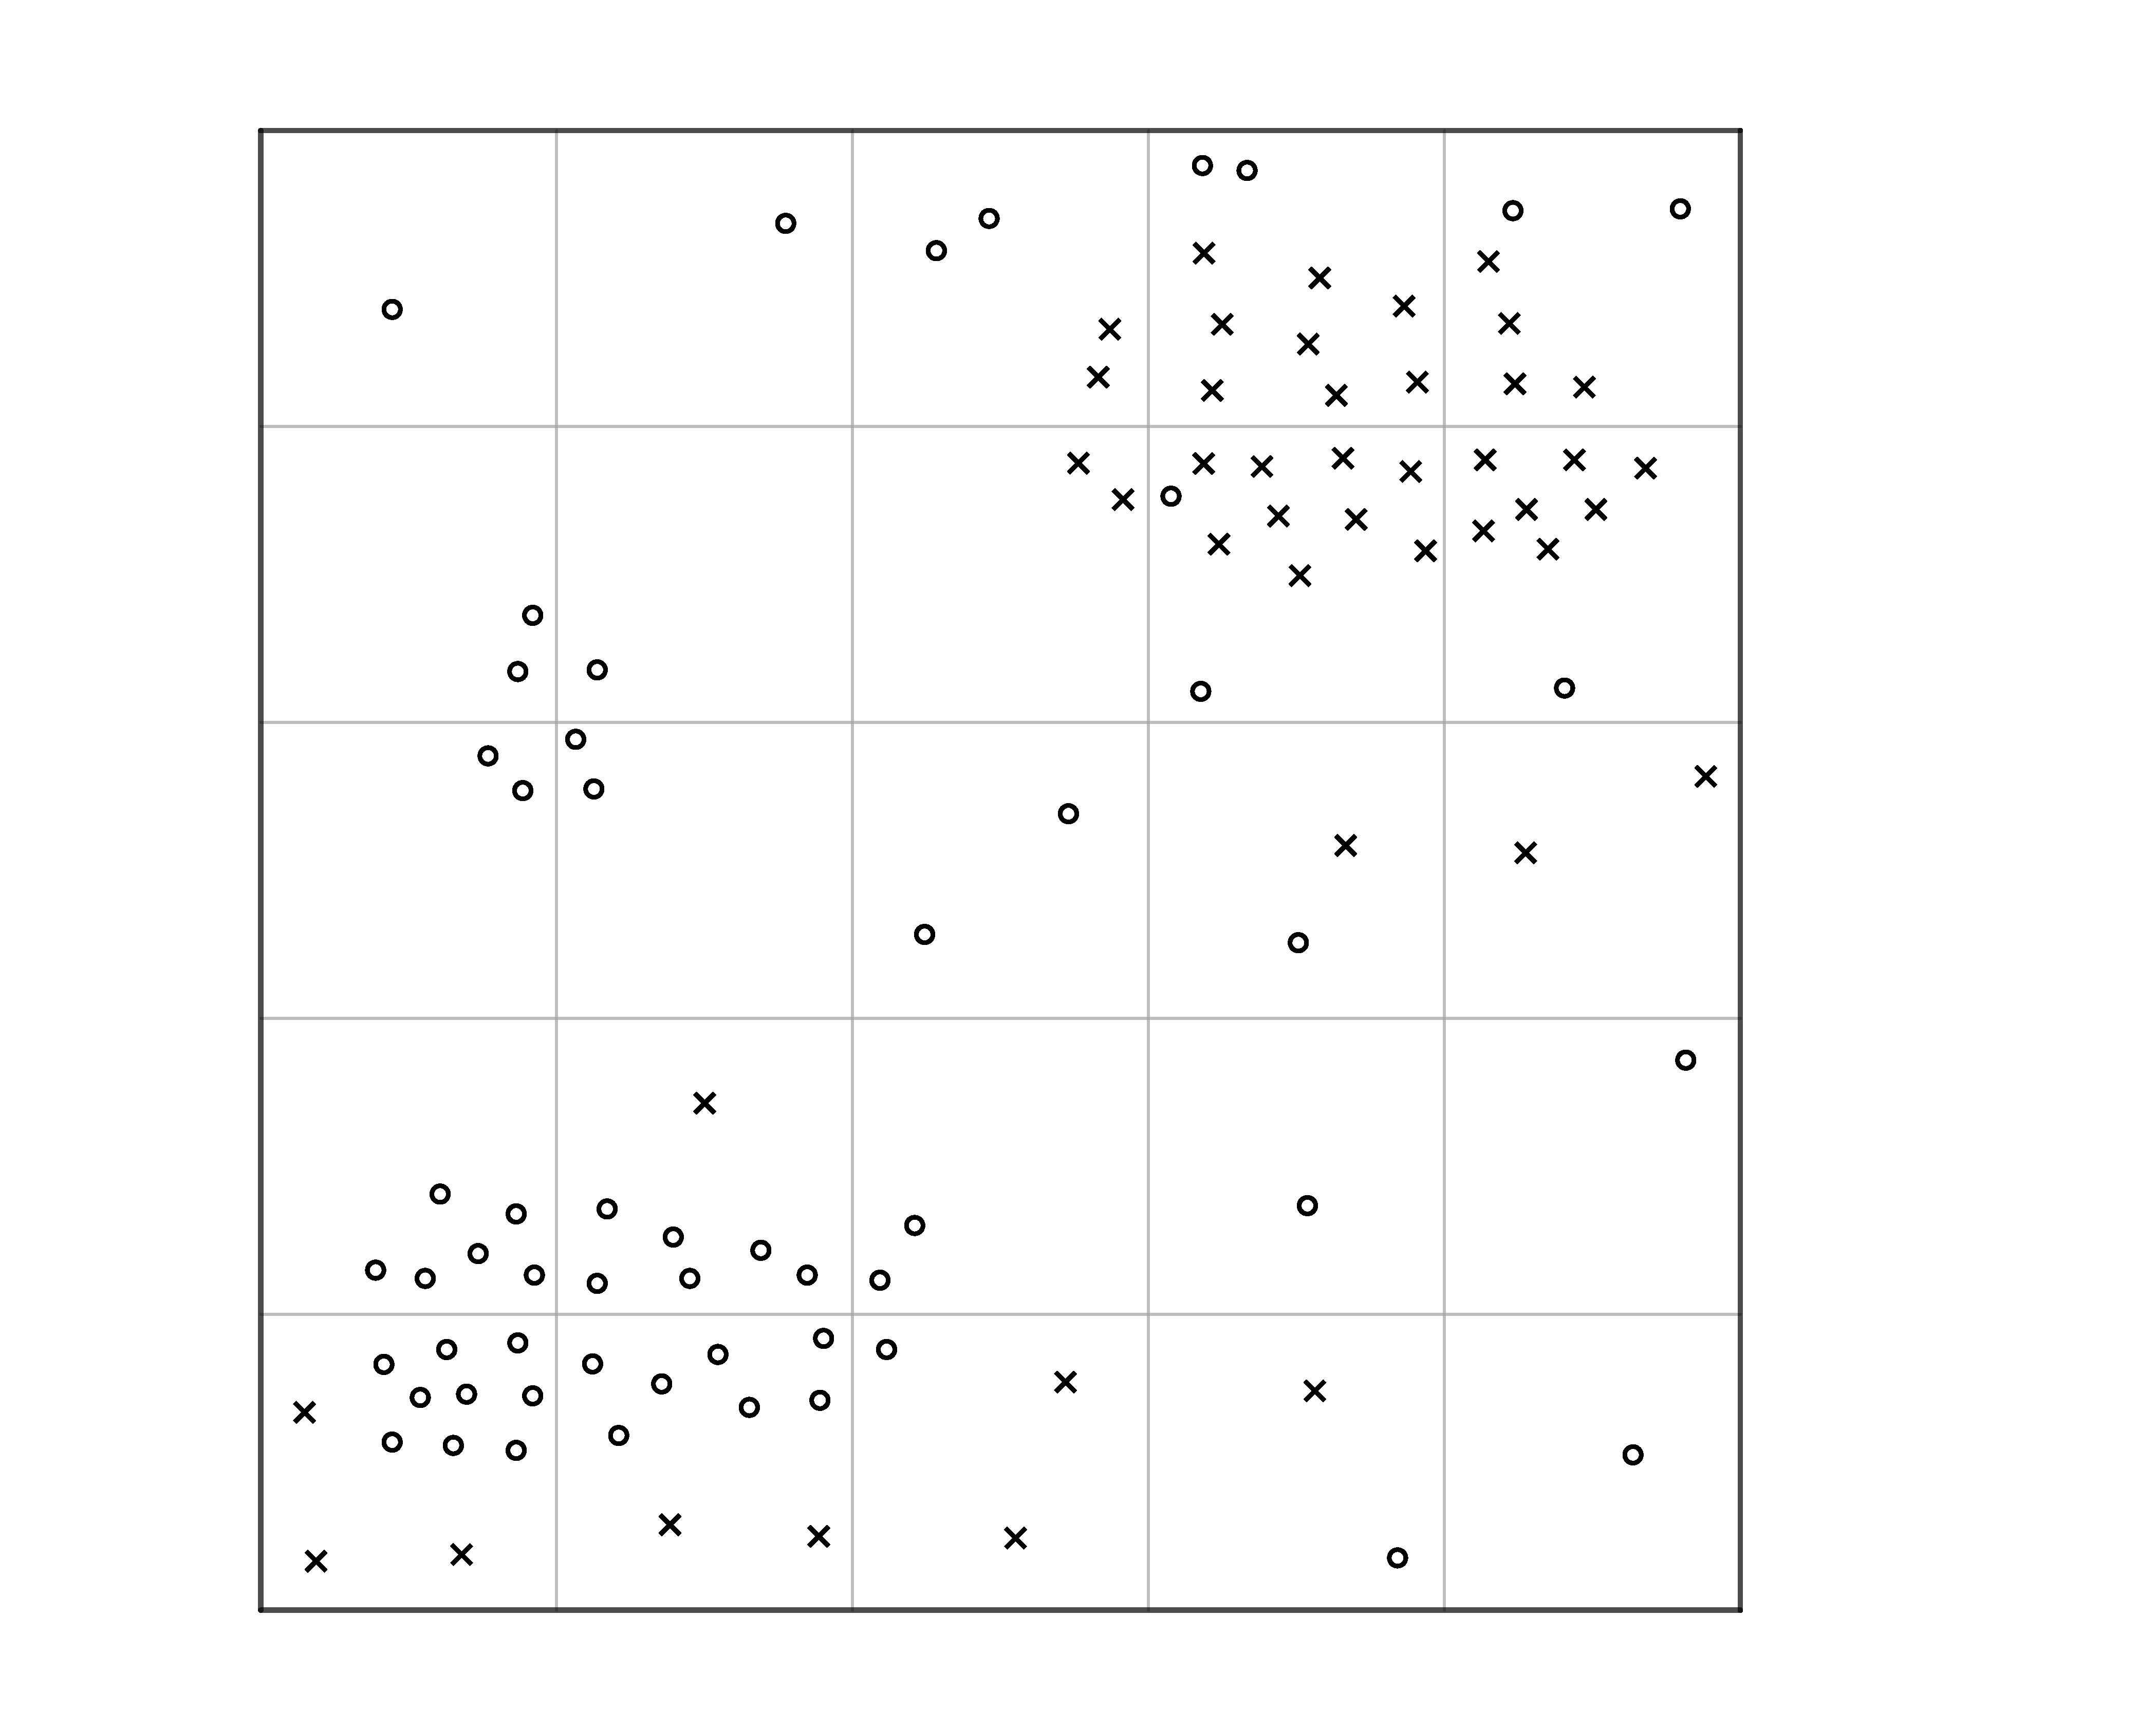
\includegraphics[width=2in]{assets/Gerrymandering/Gerry5x5-100-3.pdf}\\
 Total Vote Count &  Total Vote Count &  Total Vote Count\\
 X -  38& X - 31 & X  - 44\\
 O - 62 & O - 69 & O - 56
 \end{tabular}

\phChapterWorksheet{Tribe E}{Population = 120}

\begin{tabular}{c c c }

Year 1 & Year 2 & Year 3 \\
 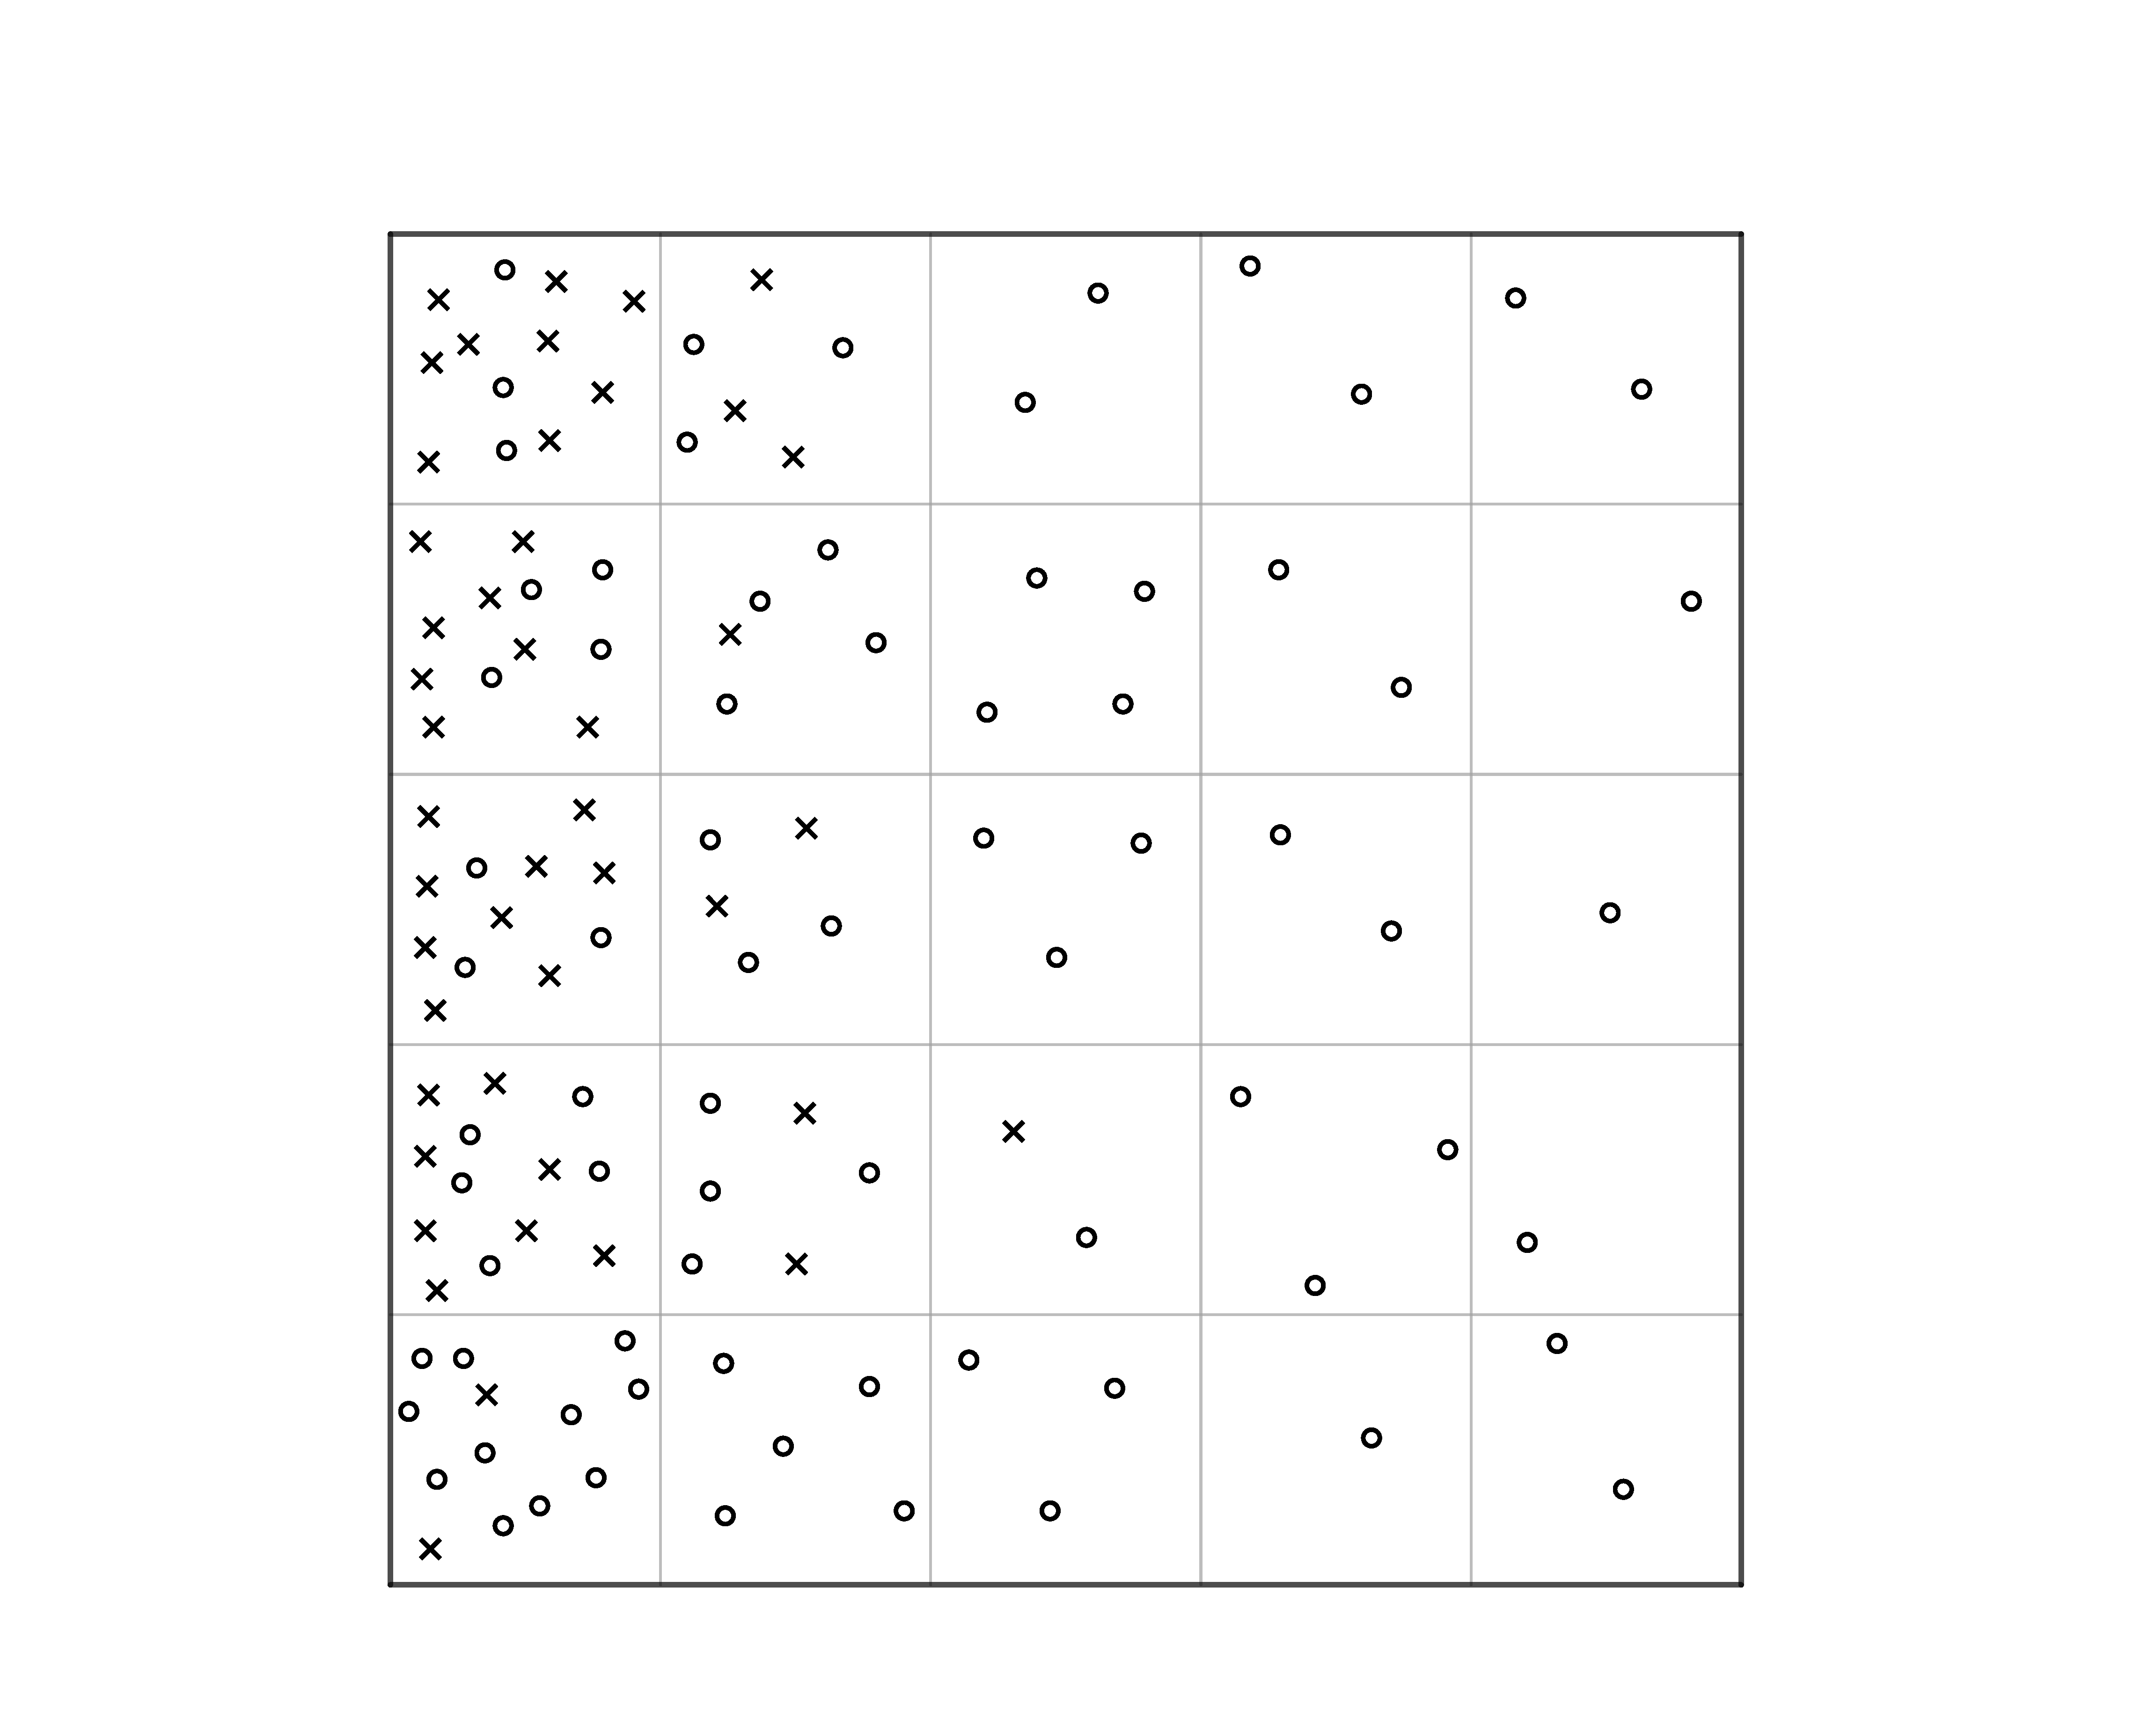
\includegraphics[width=2in]{assets/Gerrymandering/Gerry5x5-120-1.pdf} &  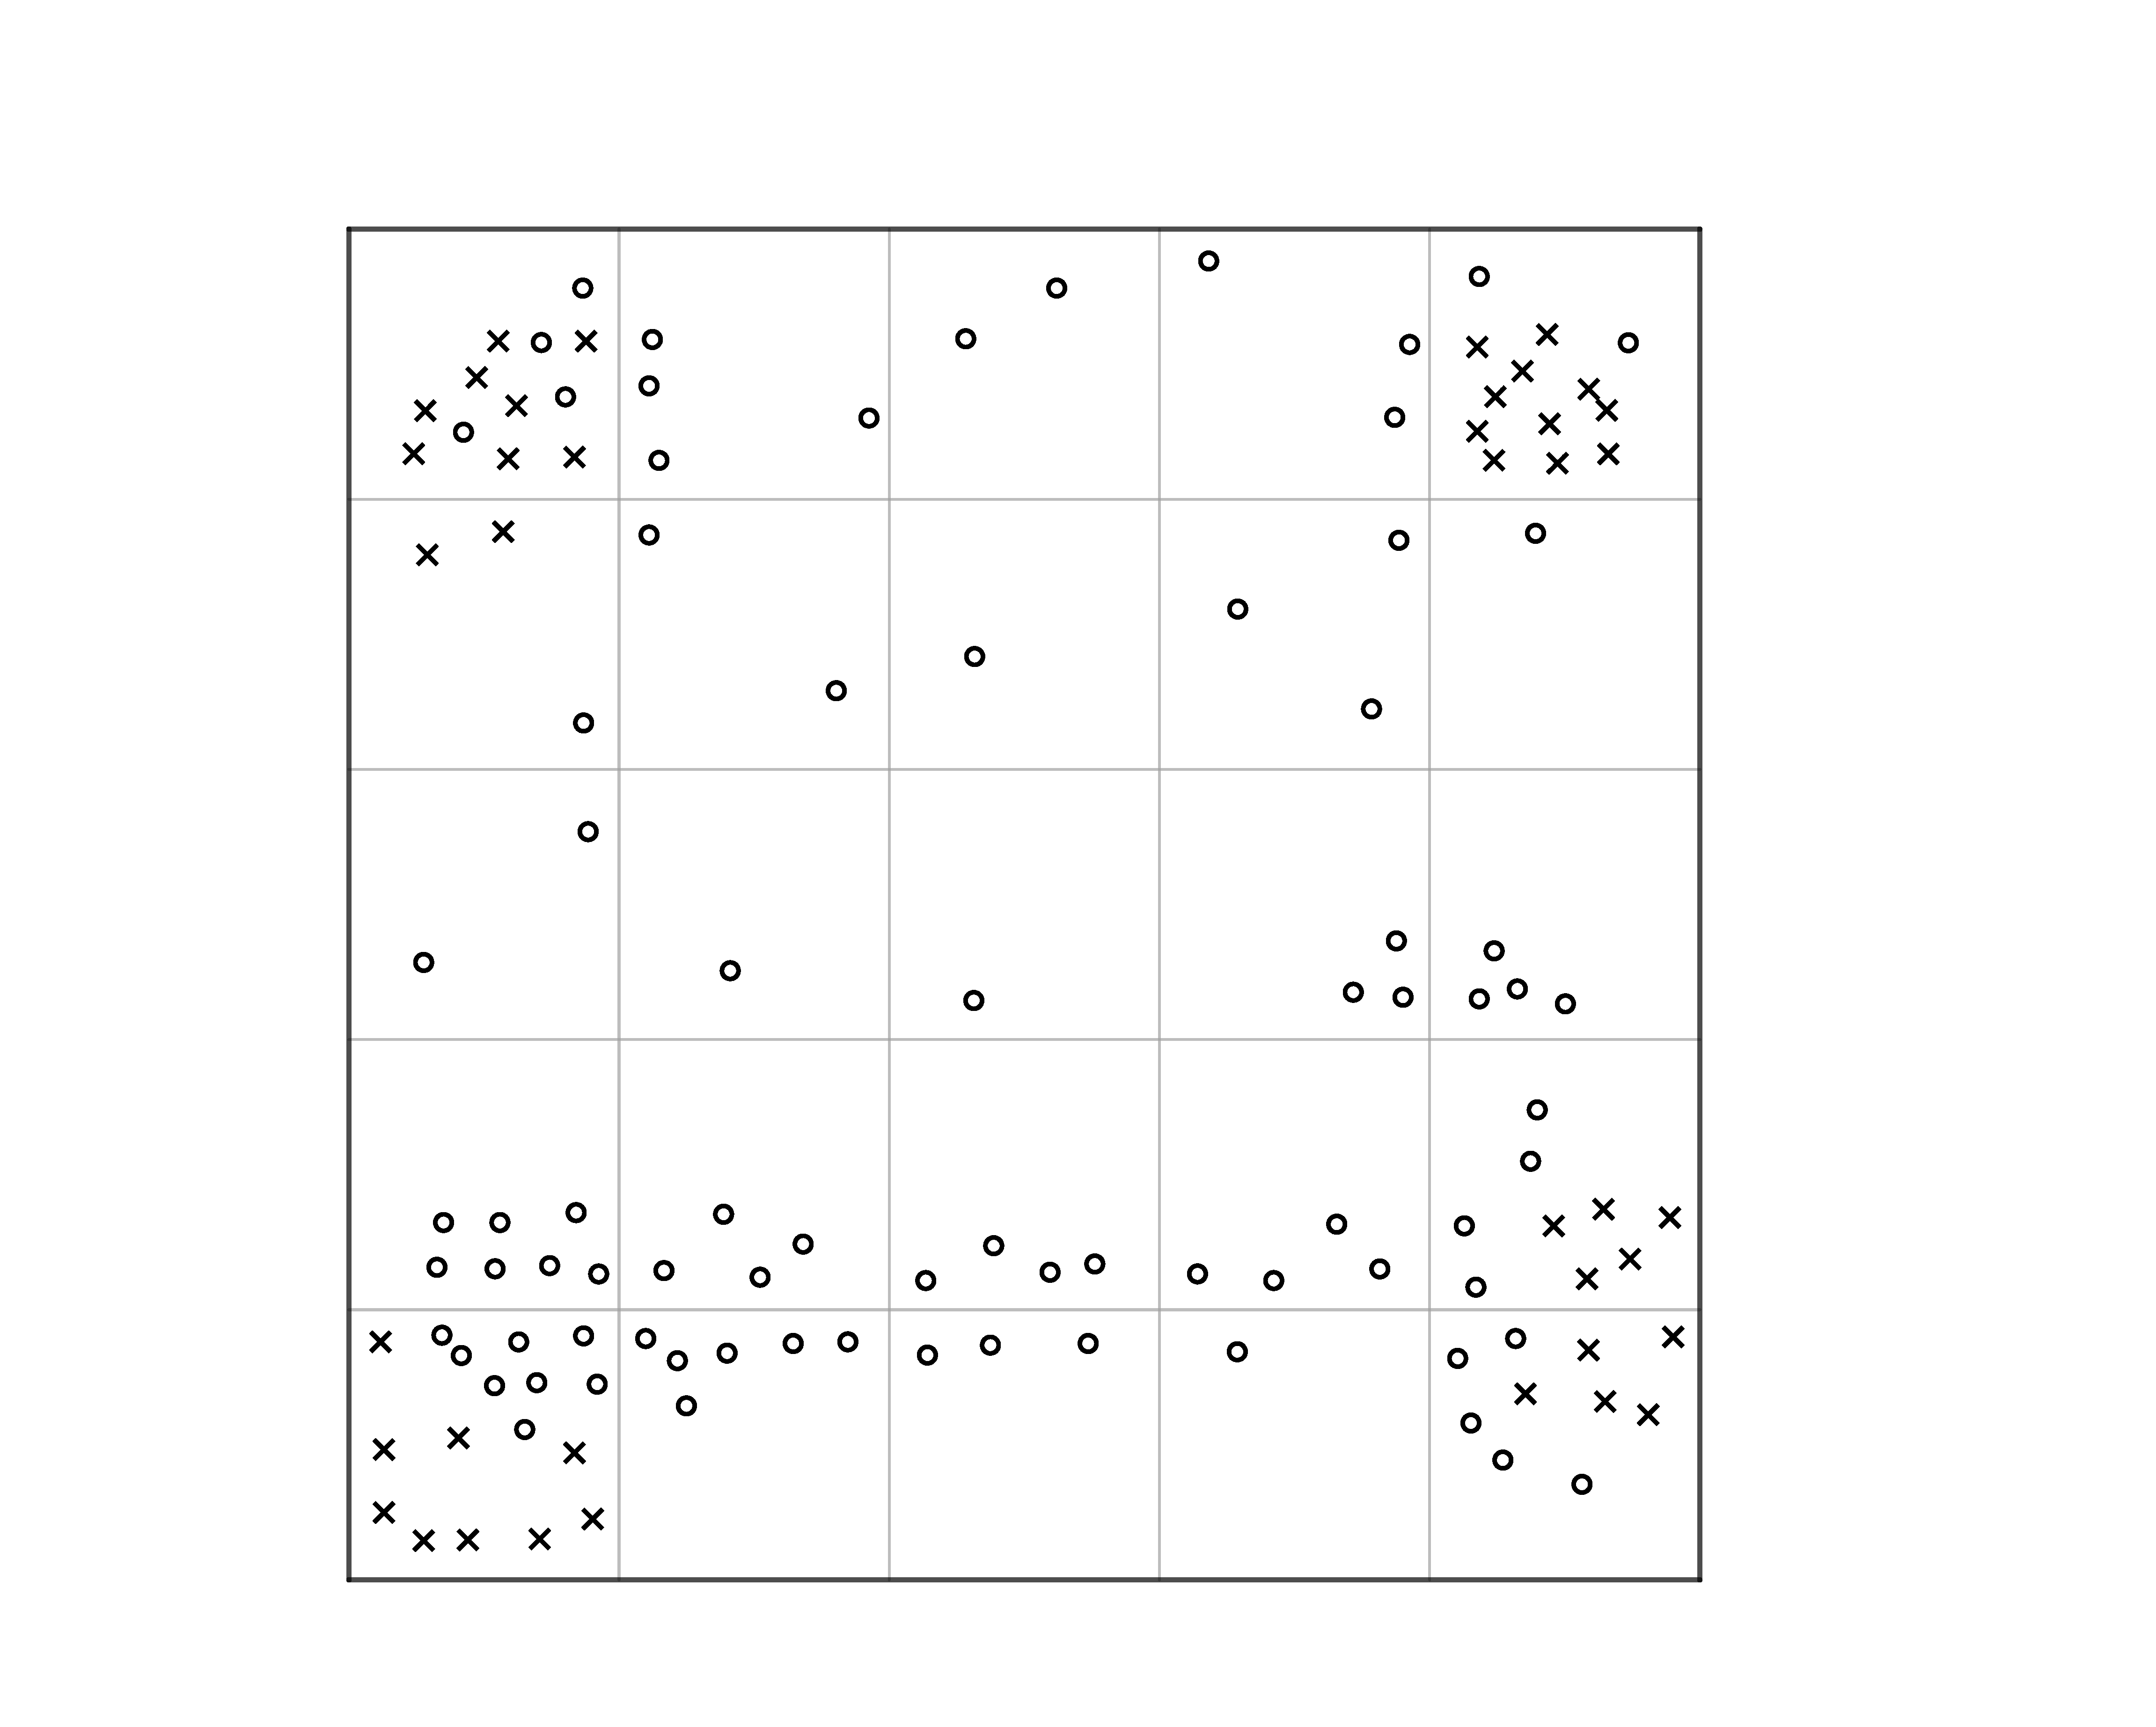
\includegraphics[width=2in]{assets/Gerrymandering/Gerry5x5-120-2.pdf} &  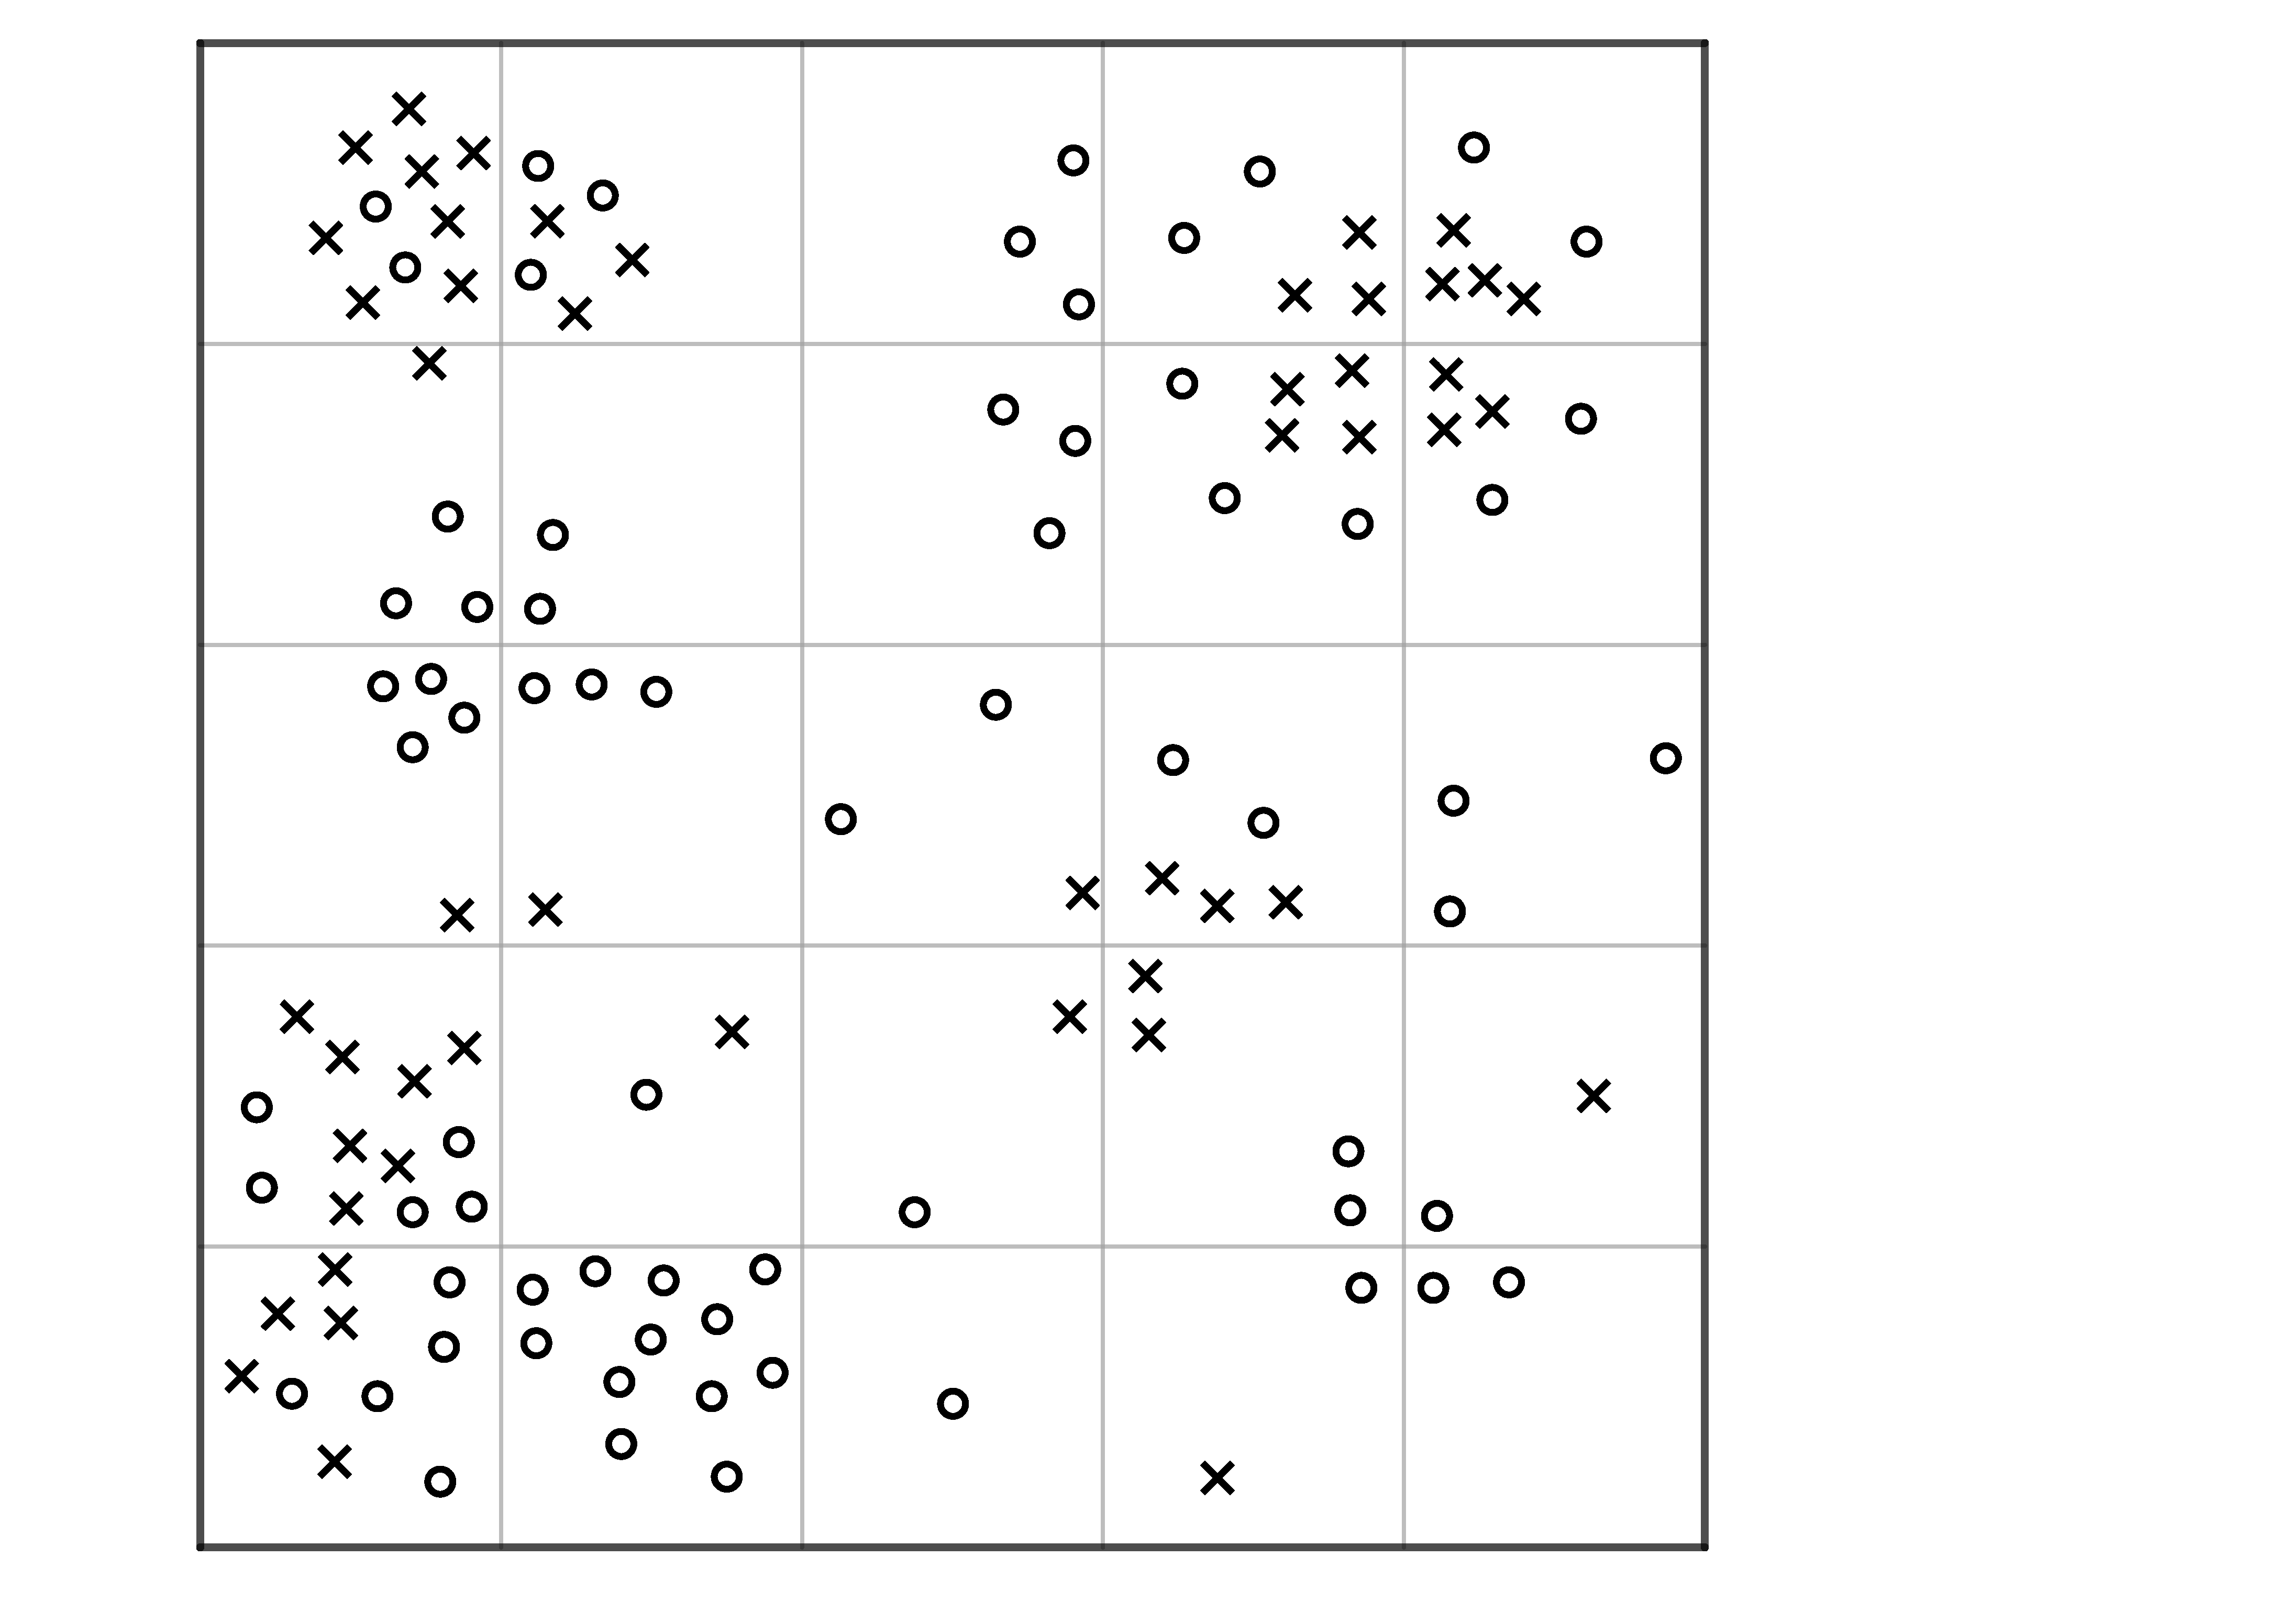
\includegraphics[width=2in]{assets/Gerrymandering/Gerry5x5-120-3.pdf}\\
 Total Vote Count &  Total Vote Count &  Total Vote Count\\
 X -  45& X - 40 & X  - 50\\
 O - 75 & O - 80 & O - 70
 \end{tabular}

\phChapterWorksheet{Tribe F}{Population = 150}

\begin{tabular}{c c c }

Year 1 & Year 2 & Year 3 \\
 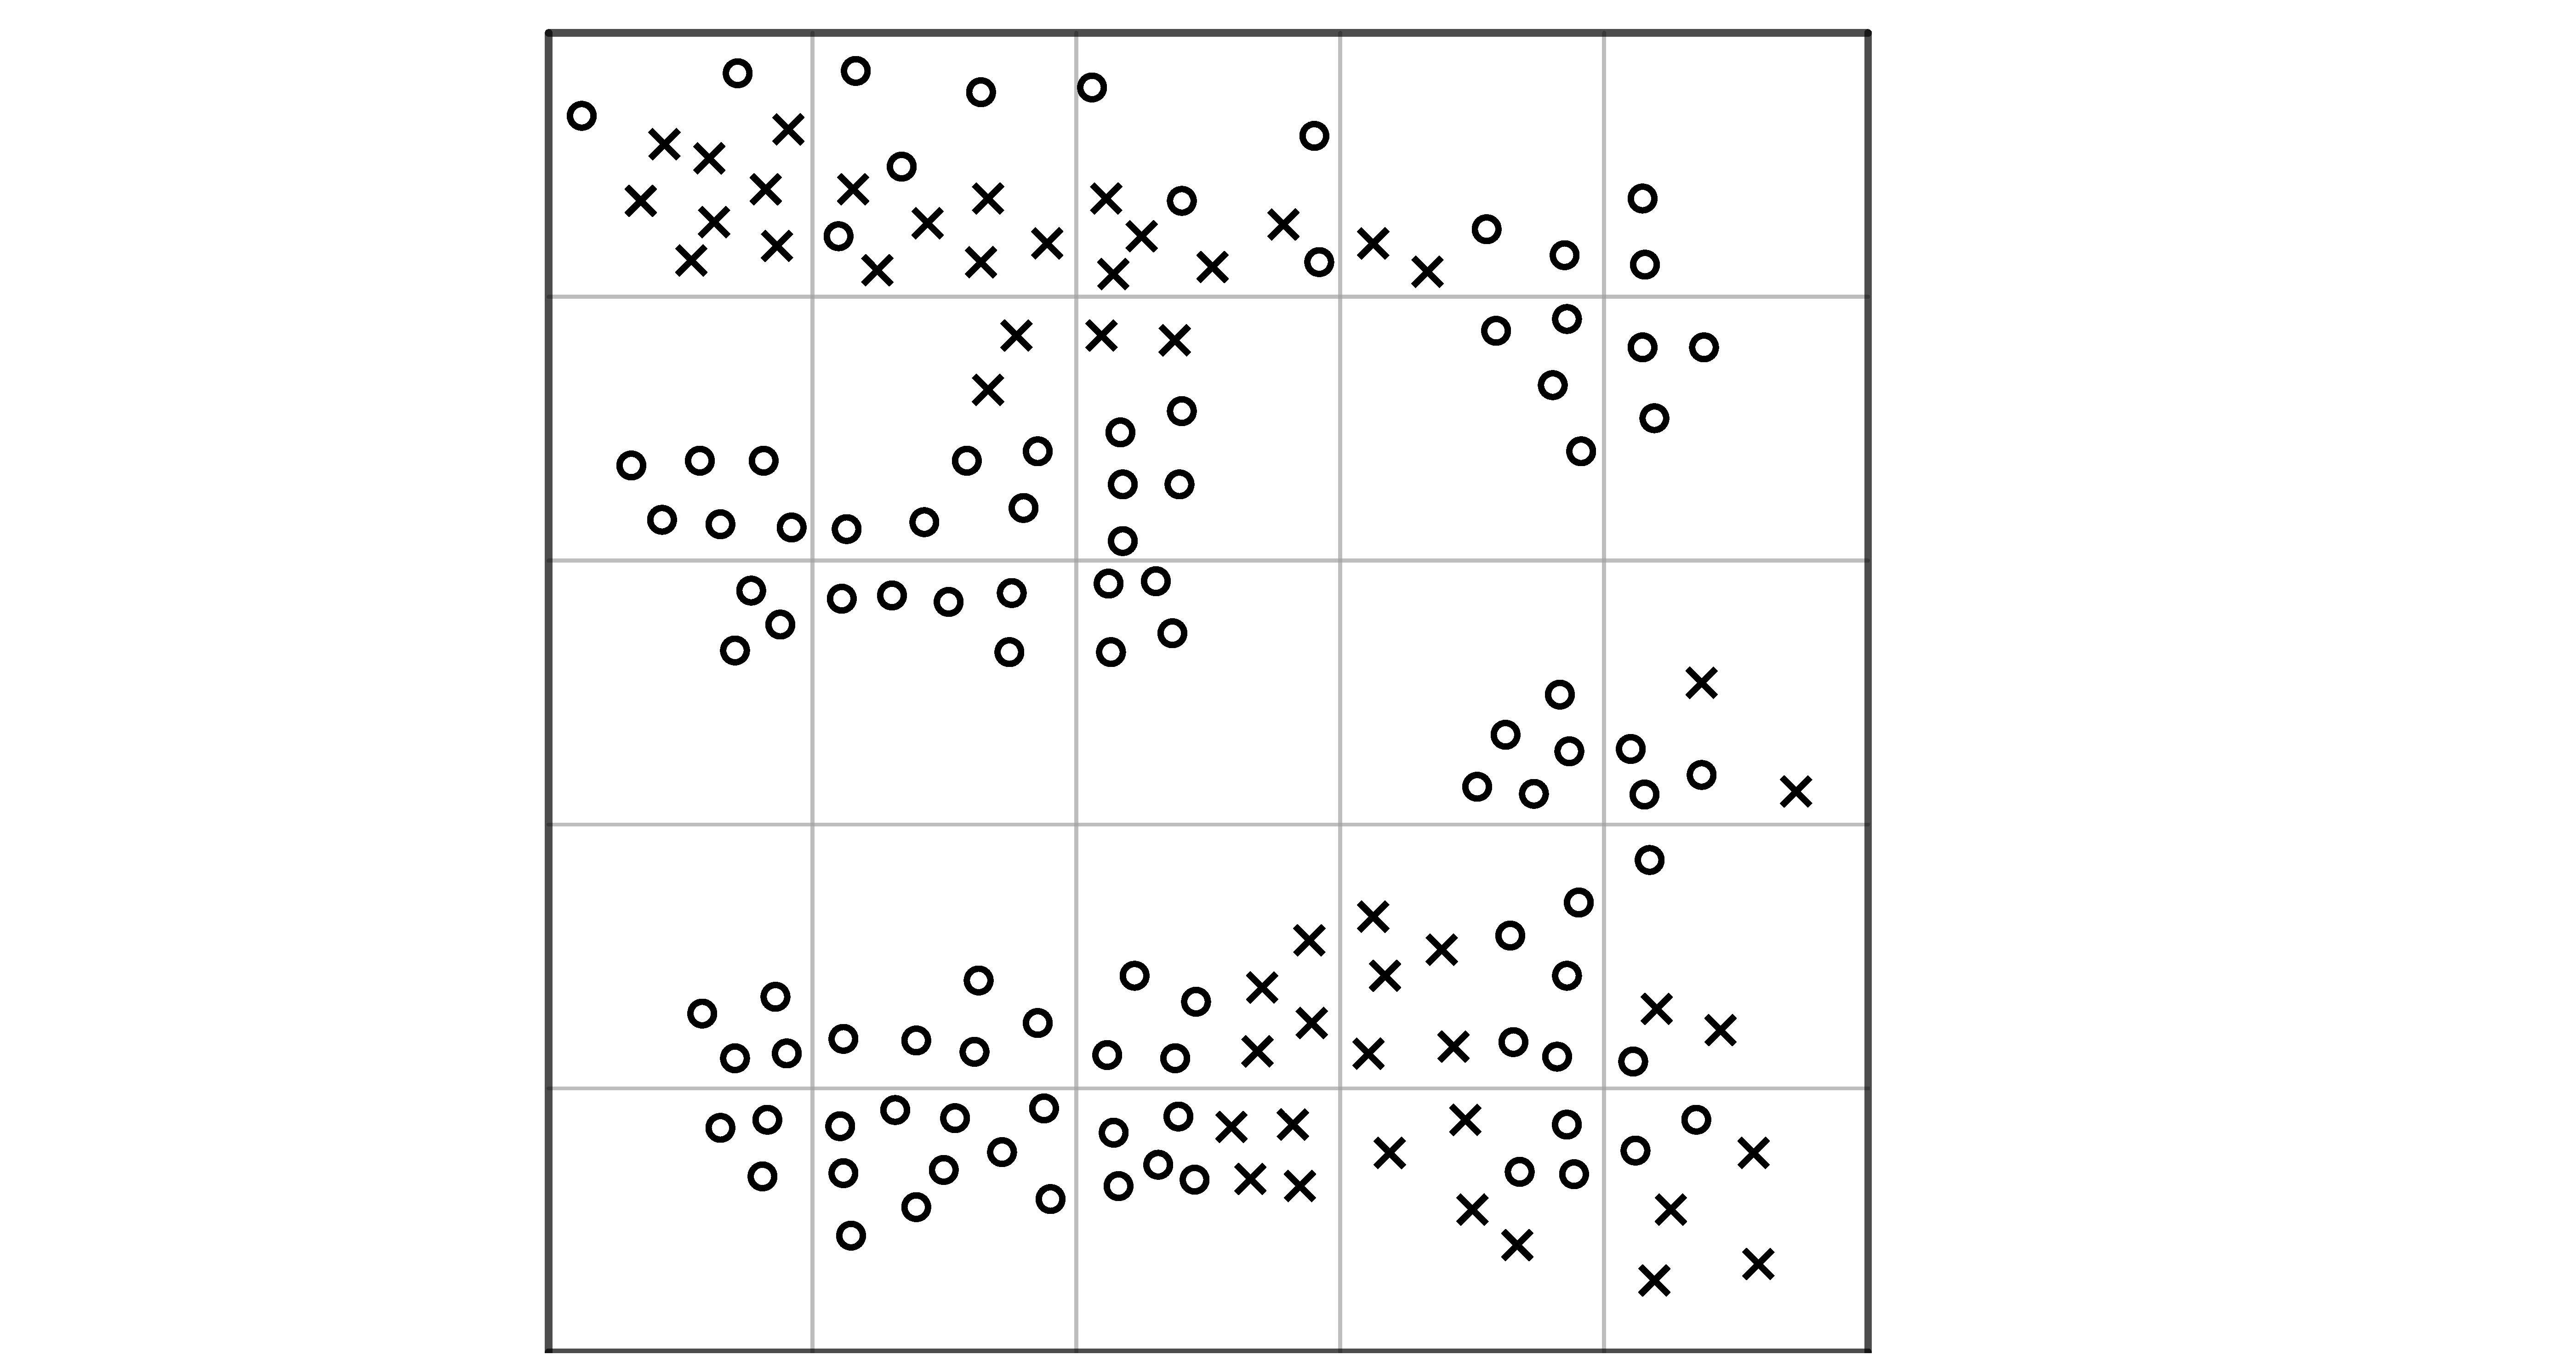
\includegraphics[width=2in]{assets/Gerrymandering/Gerry5x5-150-1.pdf} &  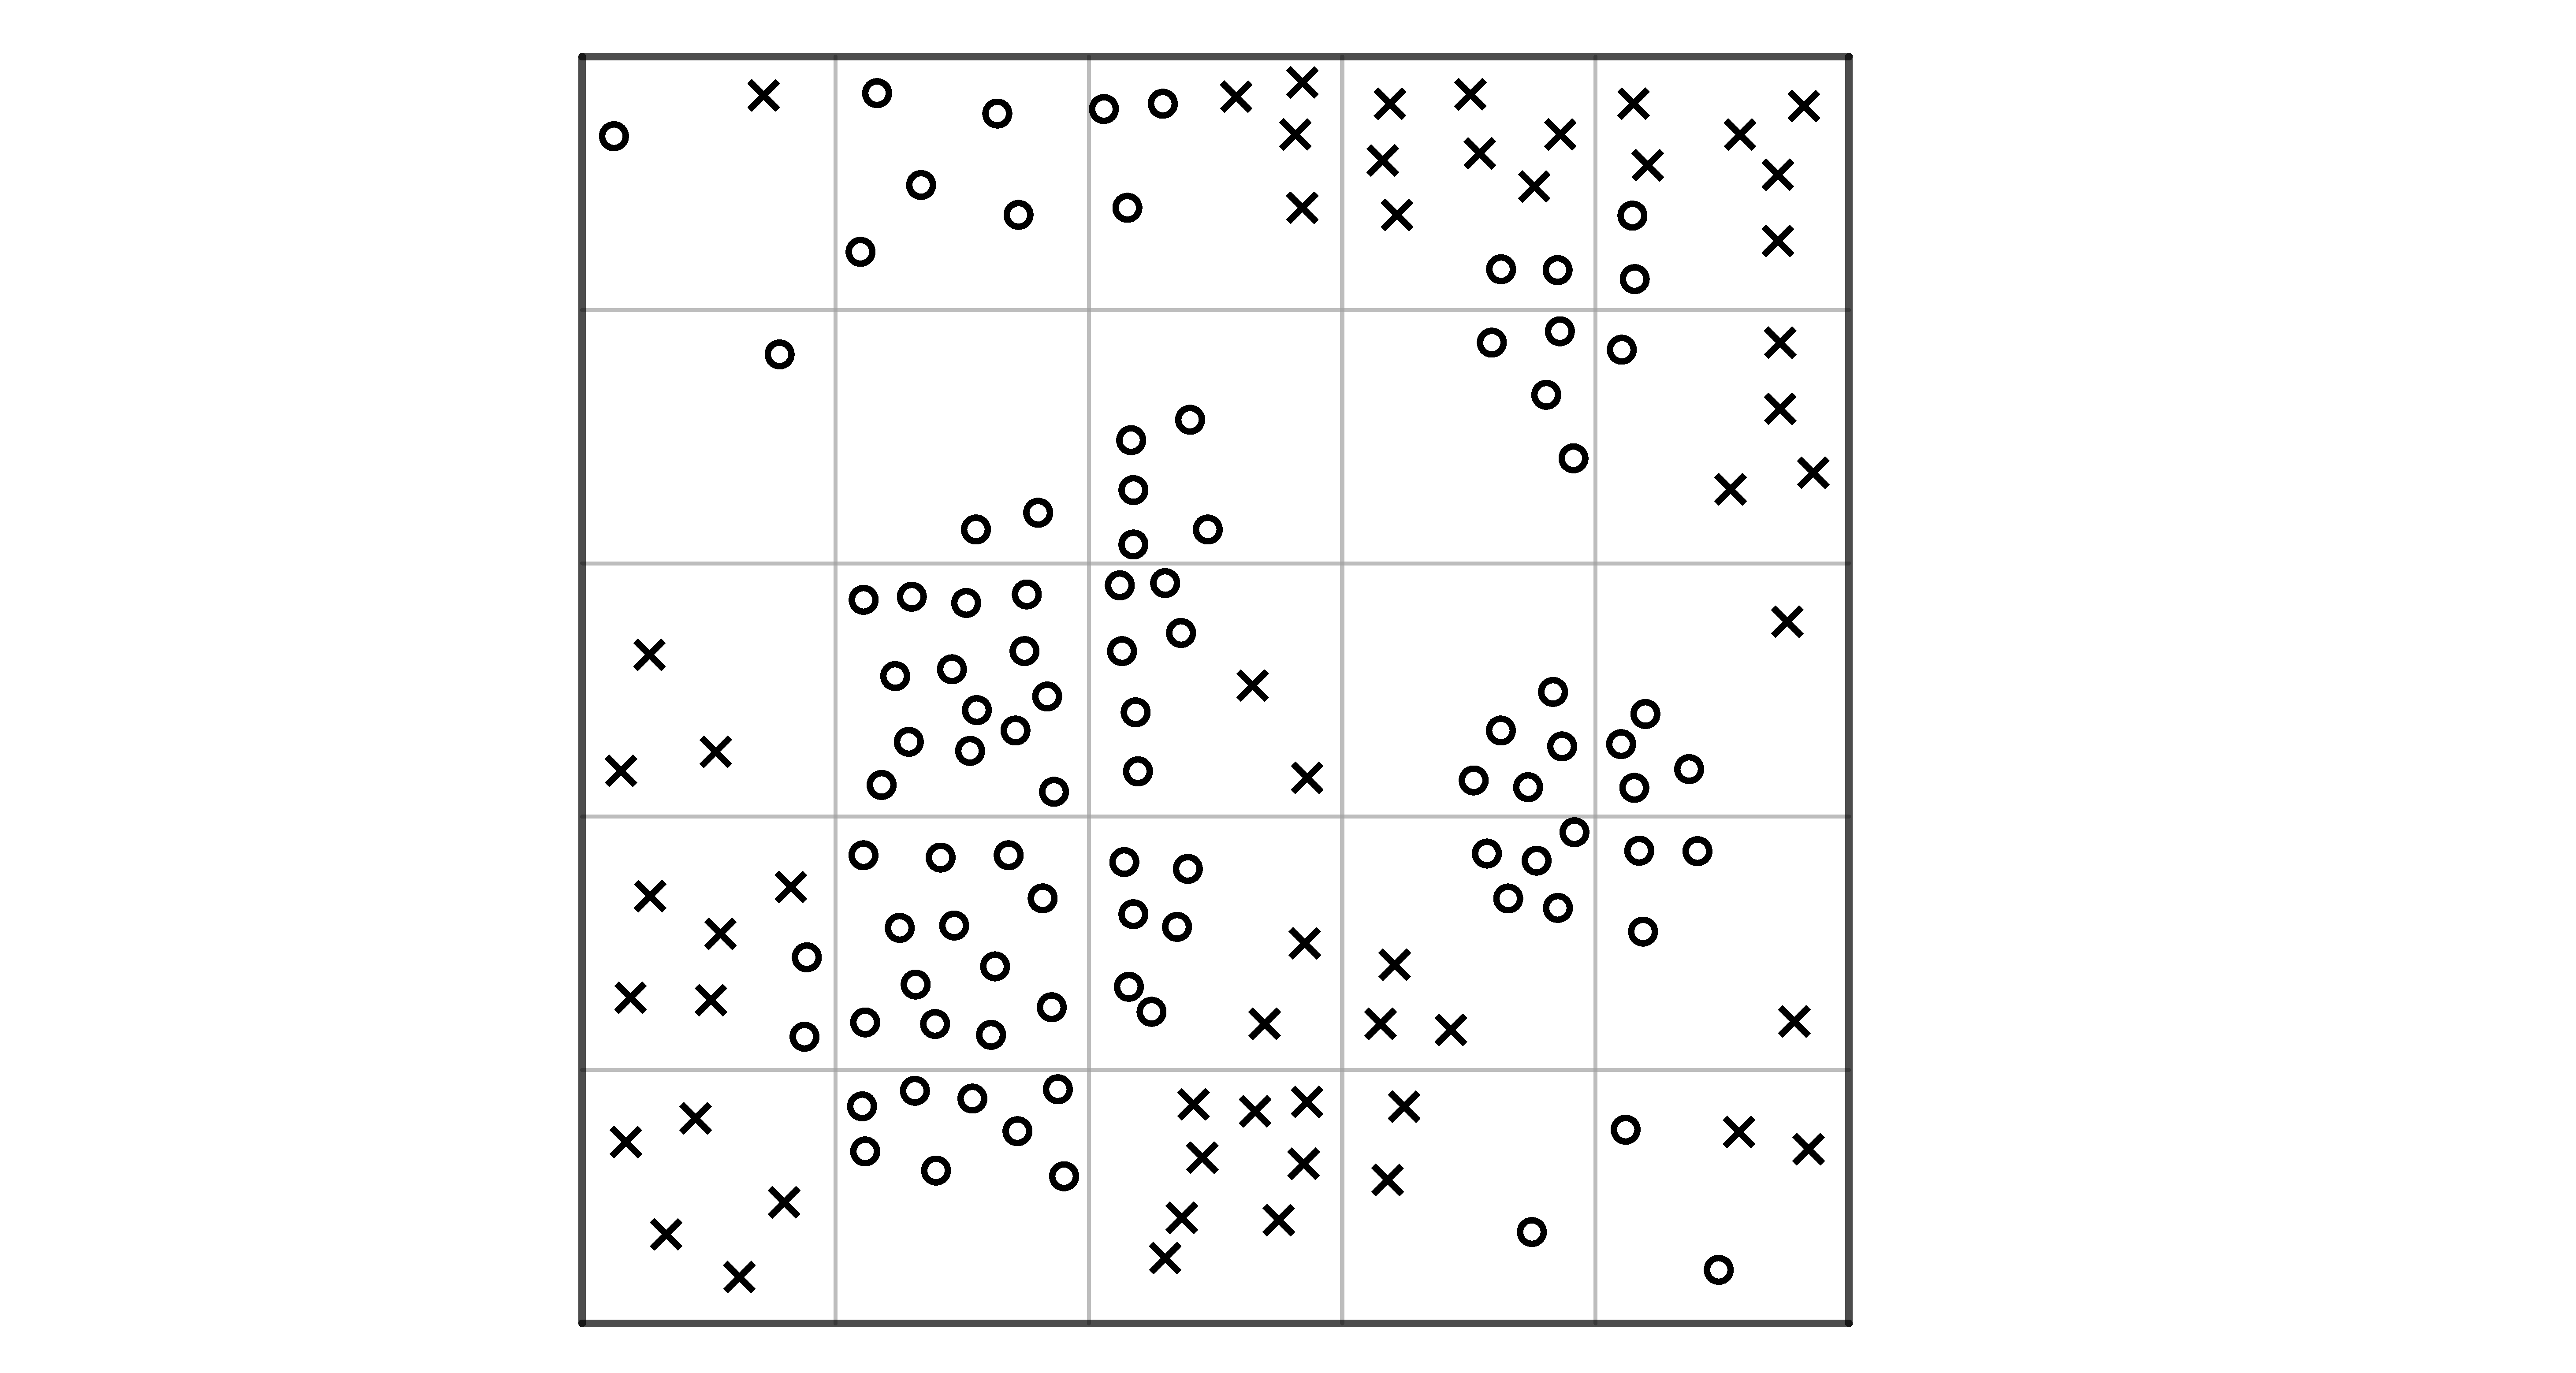
\includegraphics[width=2in]{assets/Gerrymandering/Gerry5x5-150-2.pdf} &  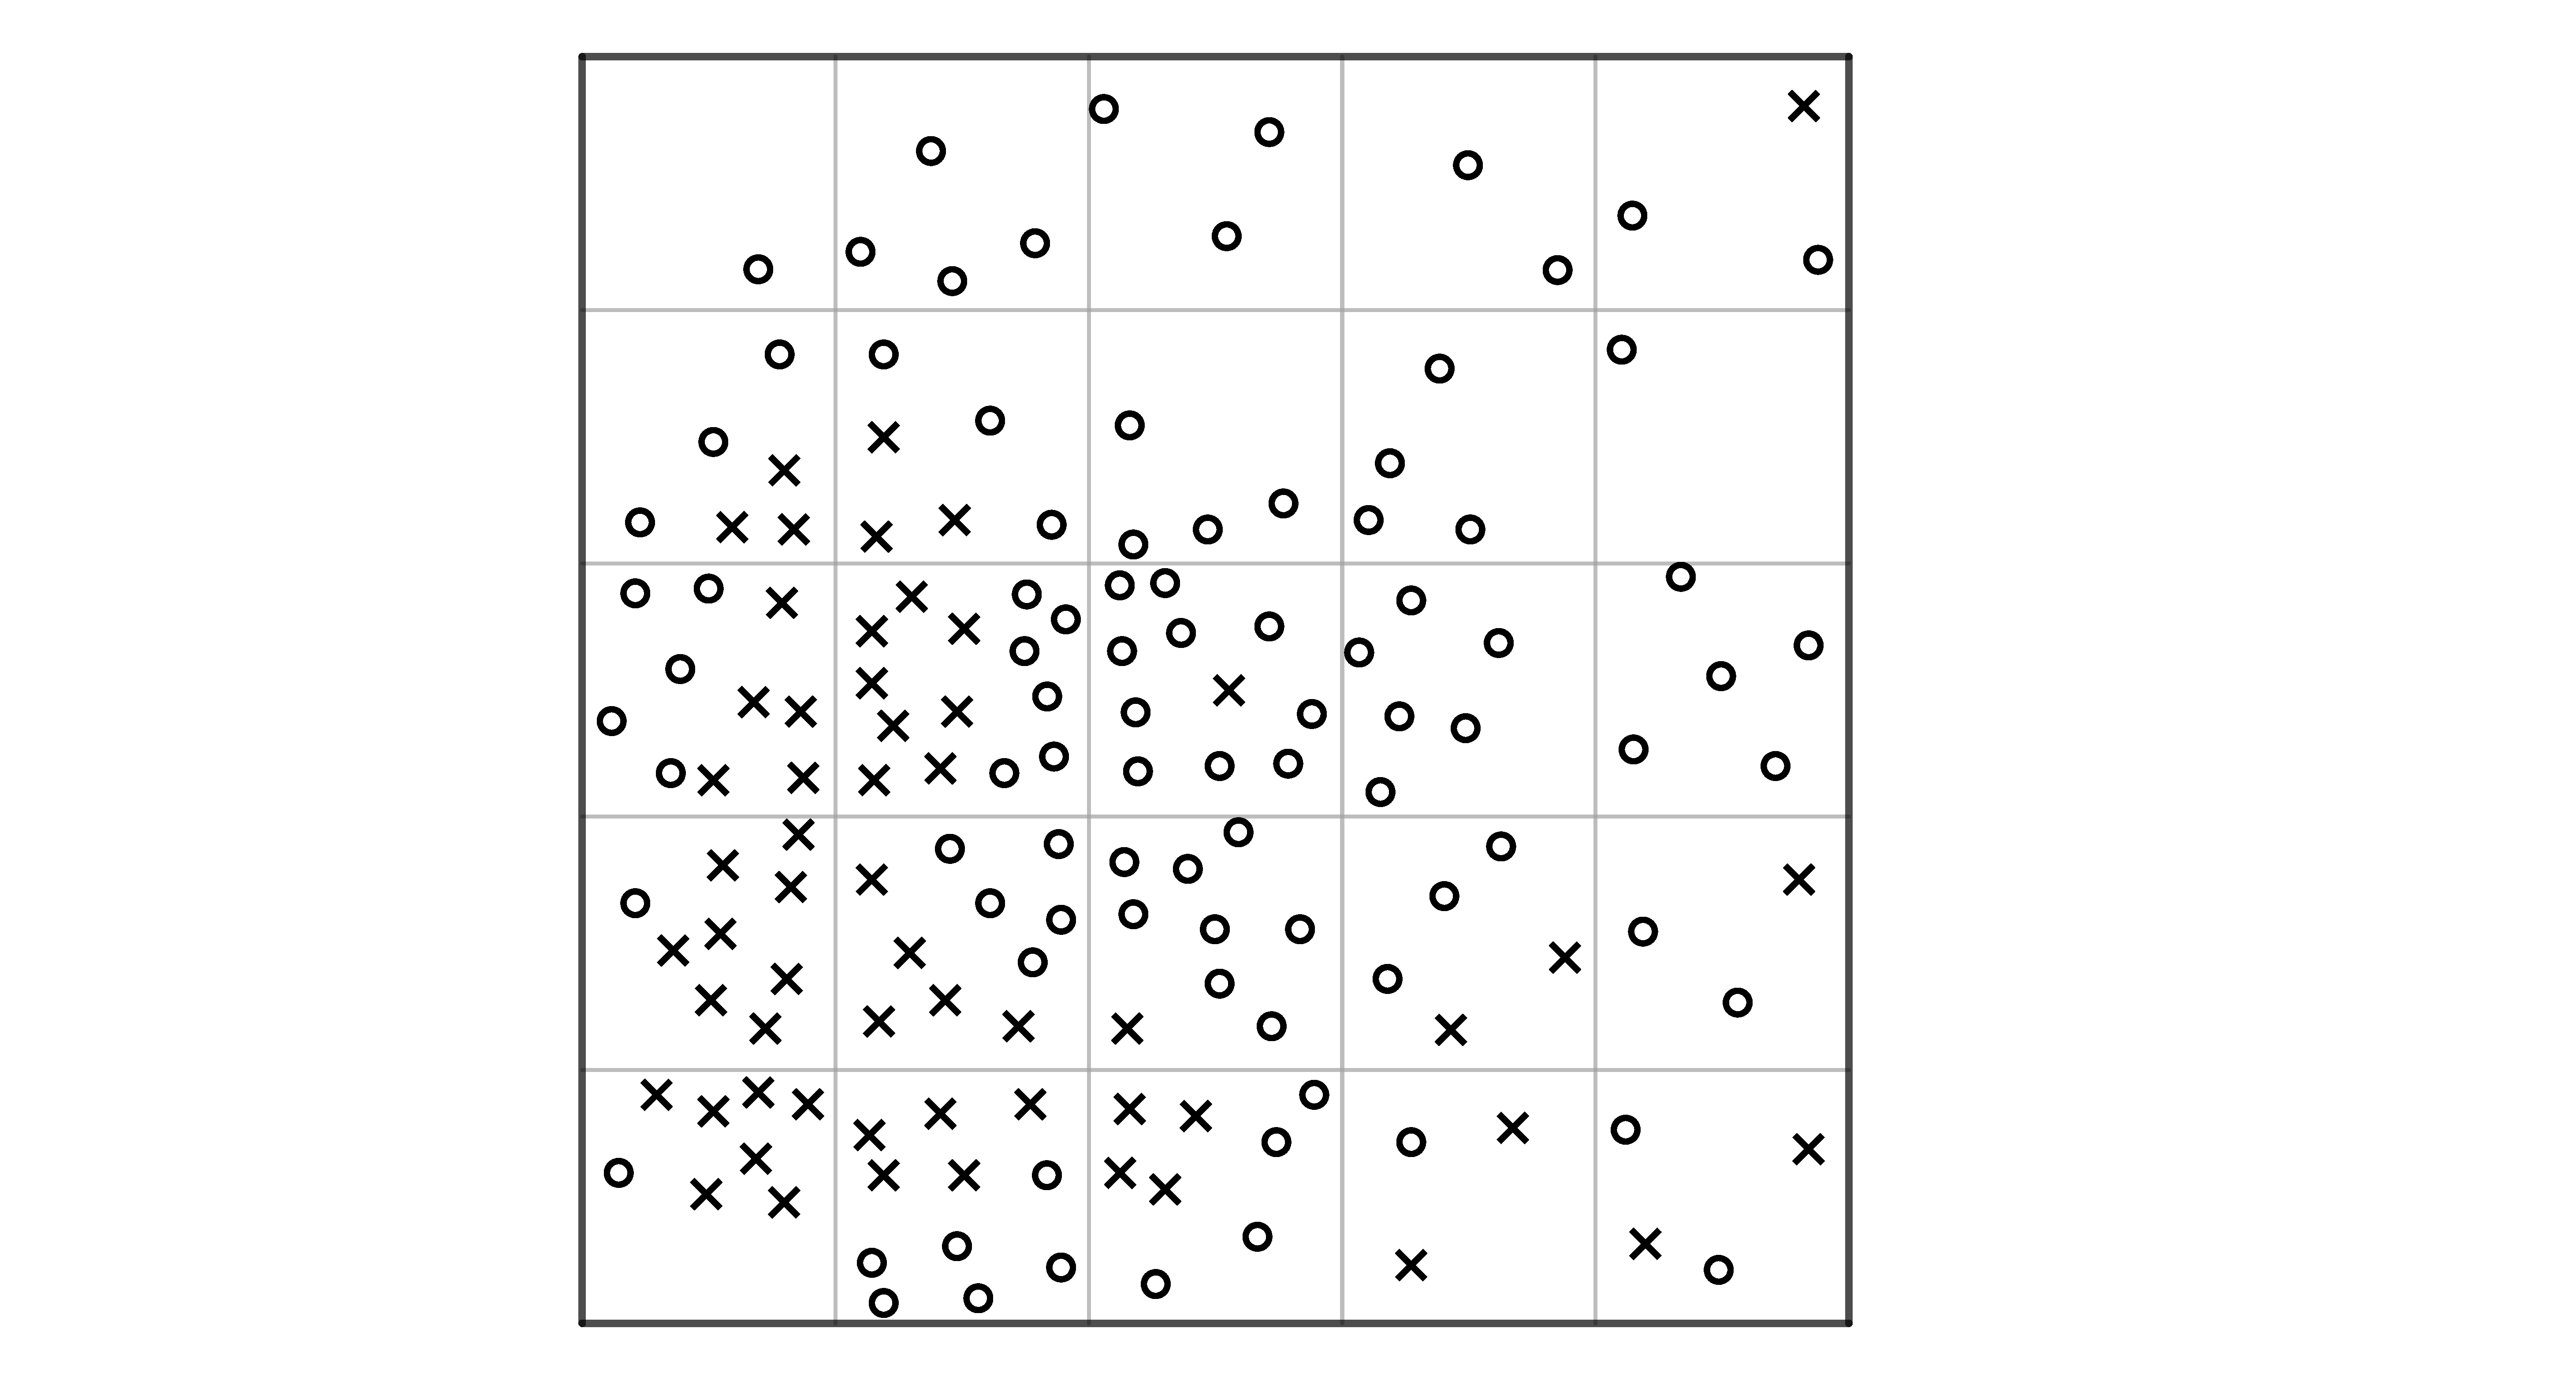
\includegraphics[width=2in]{assets/Gerrymandering/Gerry5x5-150-3.pdf}\\
 Total Vote Count &  Total Vote Count &  Total Vote Count\\
 X -  50& X - 56 & X  - 58\\
 O - 100 & O - 96 & O - 92
 \end{tabular}

\phChapterWorksheet{Journal Page 4}{}

{
  \LARGE
  \normalfont\wedn
Rulers of the Skolem People:

\renewcommand{\labelitemi}{}
\begin{itemize}
\item Throralf Apo Thue 2100 - 2050 BCE
\item Oystein Apo Skolem 2050 - 2023 BCE
\item Engstrom Apo Ore 2023 - 1969 BCE
\item Shanok Apo Ore 1969 - 1959 BCE
\item Mawort Apo Ore 1952 - 1910 BCE
\item Berkov Apo Kel 1904 - 1894 BCE
\item Knutten Apo Kel 1894 - 1885 BCE
\item Renfrow Apo Kel 1883 - 1849 BCE
\item Erbach Apo Kel 1849 - 1834 BCE
\item Guibas Apo Dheub 1830 - 1816 BCE
\item Zabala Apo Dheub 1816 - 1773 BCE
\item Gangolli Apo Dheub 1773 - 1726 BCE
\item Ramkumar Apo Lewo 1720 - 1695 BCE
\item Skraba Apo Lewo 1695 - 1687 BCE
\item Govc Apo Preis 1686 - 1675 BCE
\end{itemize}
}

\phChapterWorksheet{Cryptic Puzzle 1}{Word Graph Thing}

  %\begin{center}
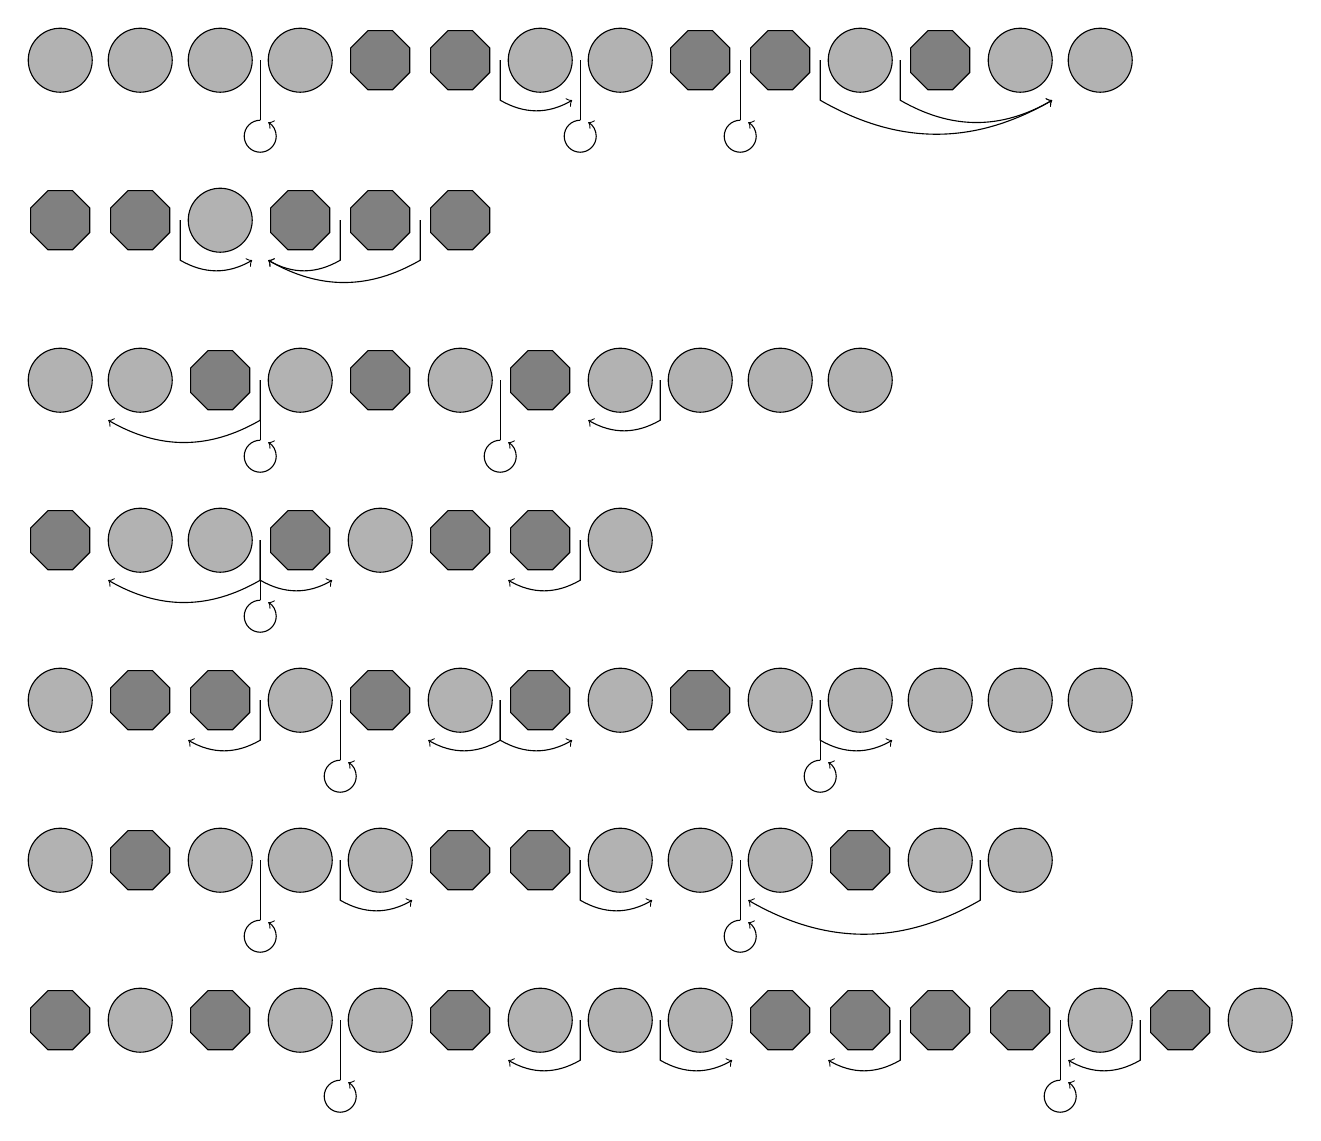
\begin{tikzpicture}[x=0.4in,y=0.4in]
% SWEATED --> SPACE
\begin{scope}[shift={(0,0)}]
\shortB\shortB\shortB
  \stStay\spaceB
\shortB\longB\longB
  \stRight{1}\spaceB
\shortB
  \stStay\spaceB
\shortB\longB
  \stStay\spaceB
\longB
  \stRight{3}\spaceB
\shortB
  \stRight{2}\spaceB
\longB\shortB\shortB
  \resetB
\end{scope}
% MATT --> GO
\begin{scope}[shift={(0,-2)}]
\longB\longB
  \stRight{1}\spaceB
\shortB\longB
  \stLeft{1}\spaceB
\longB
  \stLeft{2}\spaceB
\longB
  \resetB
\end{scope}
% URNS --> EARTH
\begin{scope}[shift={(0,-4)}]
\shortB\shortB\longB
  \stLeft{2}\stStay\spaceB
\shortB\longB\shortB
  \stStay\spaceB
\longB\shortB
  \stLeft{1}\spaceB
\shortB\shortB\shortB
  \resetB
\end{scope}
% DYE --> TITAN
\begin{scope}[shift={(0,-6)}]
\longB\shortB\shortB
  \stLeft{2}\stStay\stRight{1}\spaceB
\longB\shortB\longB\longB
  \stLeft{1}\spaceB
\shortB
  \resetB
\end{scope}
% WENCH --> ANTARES
\begin{scope}[shift={(0,-8)}]
\shortB\longB\longB
  \stLeft{1}\spaceB
\shortB
  \stStay\spaceB
\longB\shortB
  \stLeft{1}\stRight{1}\spaceB
\longB\shortB\longB\shortB
  \stStay\stRight{1}\spaceB
\shortB\shortB\shortB\shortB
  \resetB
\end{scope}
% REWIRE --> RIGEL
\begin{scope}[shift={(0,-10)}]
\shortB\longB\shortB
  \stStay\spaceB
\shortB
  \stRight{1}\spaceB
\shortB\longB\longB
  \stRight{1}\spaceB
\shortB\shortB
  \stStay\spaceB
\shortB\longB\shortB
  \stLeft{3}\spaceB
\shortB
  \resetB
\end{scope}
% CREWMEN --> CASTOR
\begin{scope}[shift={(0,-12)}]
\longB\shortB\longB\shortB
  \stStay\spaceB
\shortB\longB\shortB
  \stLeft{1}\spaceB
\shortB
  \stRight{1}\spaceB
\shortB\longB\longB
  \stLeft{1}\spaceB
\longB\longB
  \stStay\spaceB
\shortB
  \stLeft{1}\spaceB
\longB\shortB
  \resetB
\end{scope}
\end{tikzpicture}
\end{center}

%\tikzstyle{space} = [draw, circle, dotted]
%\tikzstyle{dot} = [draw, thin, circle, fill=black]
%\tikzstyle{dash} = [thick, line width=3mm, line cap=round]
%
%\newcommand{\dit}{ ++(1,0) node[dot]{} }
%\newcommand{\dah}{ ++(1,0) -- ++(2,0) }
%
%
%\newcommand{\drop}[1]{
%	\draw[->] (#1-0.5,0.5) node[space] {} -- ++(0,-2) node[space] {};
%	}
%\newcommand{\bend}[2]{
%	\draw[->] (#1-0.5,0.5) node[space] {} -- ++(0,-1) -- ++(#2,-1) node[space] {};
%	}
%
%\newcommand{\dex}[1] {++(2,-1.3) node {\sffamily\Large#1};}
%
%% SWEATED --> SPACE
%\begin{tikzpicture}[x=0.2in,y=0.2in]
%	\draw[dash] (-1,0){}
%		\dit \dit \dit %S
%		\dit \dah \dah %W
%		\dit %E
%		\dit \dah %A
%		\dah %T
%		\dit %E
%		\dah \dit \dit %D
%		\dex{2};
%	\drop{3};
%	\bend{10}{1};
%	\drop{11};
%	\drop{15};
%	\bend{18}{5};
%	\bend{19}{4};
%\end{tikzpicture}
%	
%
%\vspace{0.4in}
%
%% MATT --> GO
%\begin{tikzpicture}[x=0.2in,y=0.2in]
%	\draw[dash] (-1,0){}
%		\dah \dah %M
%		\dit \dah %A
%		\dah %T
%		\dah %T
%		\dex{2}
%		;
%	\bend{6}{1};
%	\bend{10}{-3};
%	\bend{13}{-6};
%\end{tikzpicture}
%
%\vspace{0.4in}
%
%% URNS --> EARTH
%\begin{tikzpicture}[x=0.2in,y=0.2in]
%	\draw[dash] (-1,0){}
%		\dit \dit \dah %U
%		\dit \dah \dit %R
%		\dah \dit %N
%		\dit \dit \dit %S
%		\dex{3}
%		;
%	\bend{5}{-4};
%	\drop{5};
%	\drop{10};
%	\bend{14}{-1};
%\end{tikzpicture}
%
%\vspace{0.4in}
%
%% DYE --> TITAN
%\begin{tikzpicture}[x=0.2in,y=0.2in]
%	\draw[dash] (-1,0){}
%		\dah \dit \dit %D
%		\dah \dit \dah \dah %Y
%		\dit %E
%		\dex{3}
%		;
%	\bend{5}{-2};
%	\drop{5};
%	\bend{5}{3};
%	\bend{15}{-3};
%\end{tikzpicture}
%
%\vspace{0.4in}
%
%% WENCH --> ANTARES
%\begin{tikzpicture}[x=0.2in,y=0.2in]
%	\draw[dash] (-1,0){}
%		\dit \dah \dah %W
%		\dit %E
%		\dah \dit %N
%		\dah \dit \dah \dit %C
%		\dit \dit \dit \dit %H
%		\dex{1}
%		;
%	\bend{7}{-3};
%	\drop{8};
%	\bend{12}{-1};
%	\bend{12}{3};
%	\drop{20};
%	\bend{20}{1};
%\end{tikzpicture}
%
%\vspace{0.4in}
%
%% REWIRE --> RIGEL
%\begin{tikzpicture}[x=0.2in,y=0.2in]
%	\draw[dash] (-1,0){}
%		\dit \dah \dit %R
%		\dit %E
%		\dit \dah \dah %W
%		\dit \dit %I
%		\dit \dah \dit %R
%		\dit %E
%		\dex{5}
%		;
%	\drop{5};
%	\bend{6}{1};
%	\bend{13}{1};
%	\drop{15};
%	\bend{20}{-5};
%\end{tikzpicture}
%
%\vspace{0.4in}
%
%% CREWMEN --> CASTOR
%\begin{tikzpicture}[x=0.2in,y=0.2in]
%	\draw[dash] (-1,0){}
%		\dah \dit \dah \dit %C
%		\dit \dah \dit %R
%		\dit %E
%		\dit \dah \dah %W
%		\dah \dah %M
%		\dit %E
%		\dah \dit %N
%		\dex{3}
%		;
%	\drop{8};
%	\bend{13}{-1};
%	\bend{14}{1};
%	\bend{21}{-3};
%	\drop{27};
%	\bend{28}{-1};
%\end{tikzpicture}


\phChapterWorksheet{Cryptic Puzzle 2}{Switchboard}

  %\begin{center}
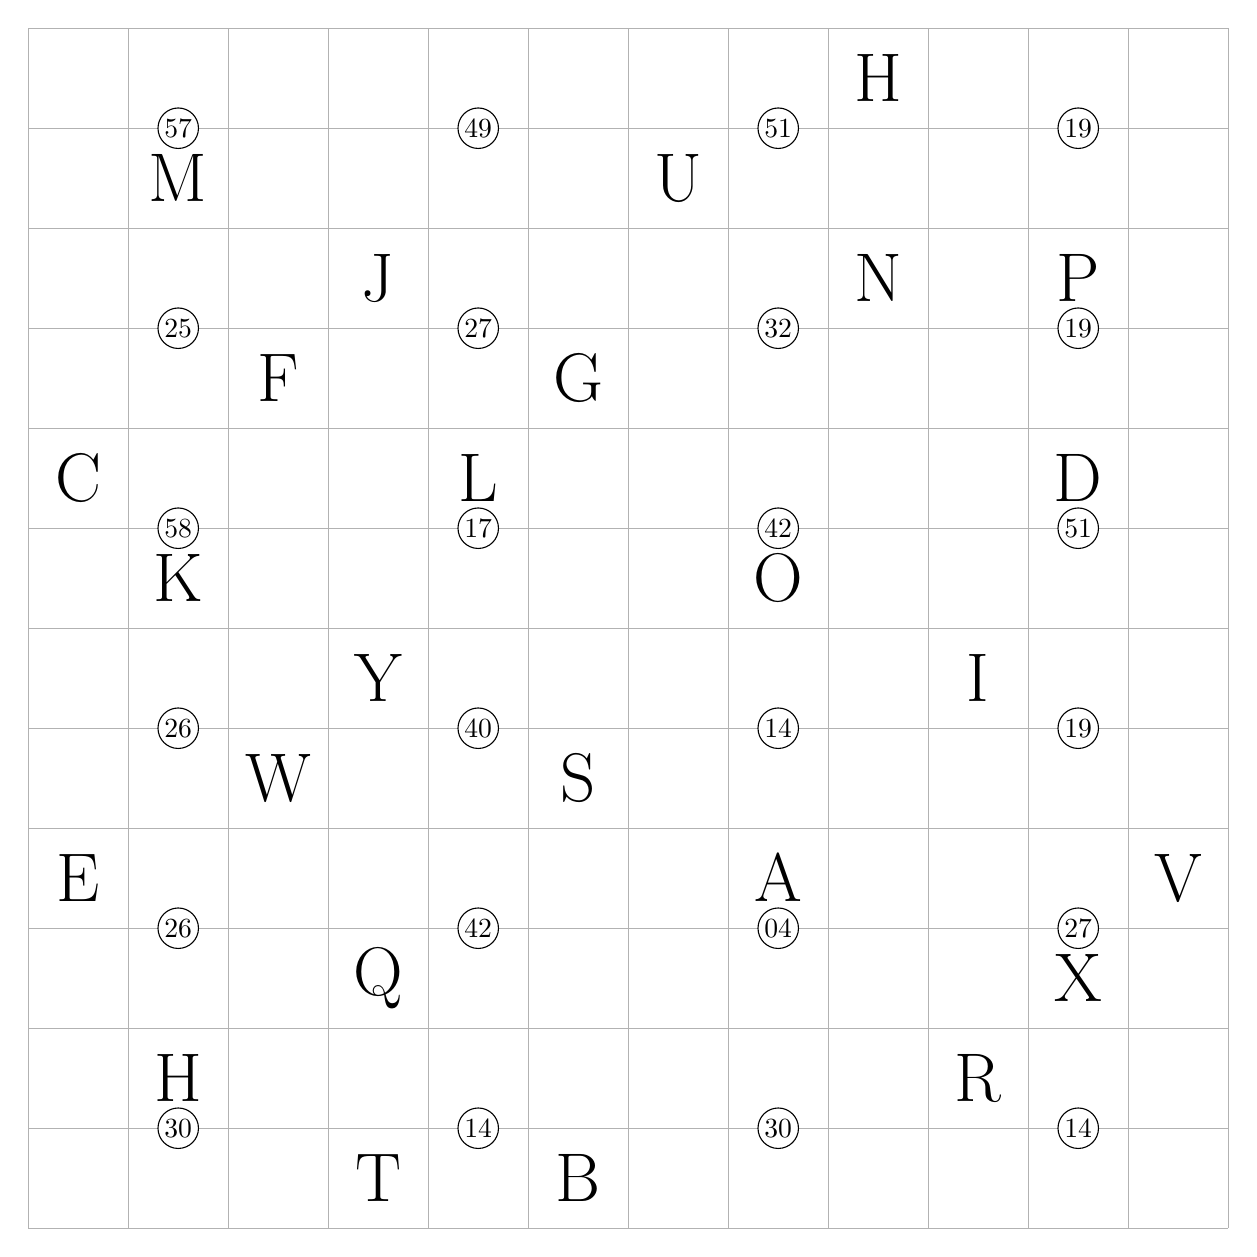
\begin{tikzpicture}[x=0.5in,y=0.5in]
\fill[white] (0,0) rectangle (12,12);
\draw[step=1,black!30] (0,0) grid (12,12);
\node at (10.5,9.5) {\Huge P};
\node at (6.5,10.5) {\Huge U};
\node at (4.5,7.5) {\Huge L};
\node at (5.5,4.5) {\Huge S};
\node at (7.5,3.5) {\Huge A};
\node at (9.5,1.5) {\Huge R};
% distractors
\node at (3.5,0.5) {\Huge T};
\node at (5.5,0.5) {\Huge B};
\node at (1.5,1.5) {\Huge H};
\node at (3.5,2.5) {\Huge Q};
\node at (10.5,2.5) {\Huge X};
\node at (0.5,3.5) {\Huge E};
\node at (11.5,3.5) {\Huge V};
\node at (2.5,4.5) {\Huge W};
\node at (3.5,5.5) {\Huge Y};
\node at (9.5,5.5) {\Huge I};
\node at (1.5,6.5) {\Huge K};
\node at (7.5,6.5) {\Huge O};
\node at (0.5,7.5) {\Huge C};
\node at (10.5,7.5) {\Huge D};
\node at (2.5,8.5) {\Huge F};
\node at (5.5,8.5) {\Huge G};
\node at (8.5,9.5) {\Huge N};
\node at (8.5,11.5) {\Huge H};
\node at (3.5,9.5) {\Huge J};
\node at (1.5,10.5) {\Huge M};
%numbers
\node[circle,draw=black,fill=white,inner sep=1pt] at (1.5,11) {57};
\node[circle,draw=black,fill=white,inner sep=1pt] at (4.5,11) {49};
\node[circle,draw=black,fill=white,inner sep=1pt] at (7.5,11) {51};
\node[circle,draw=black,fill=white,inner sep=1pt] at (10.5,11) {19};
\node[circle,draw=black,fill=white,inner sep=1pt] at (1.5,9) {25};
\node[circle,draw=black,fill=white,inner sep=1pt] at (4.5,9) {27};
\node[circle,draw=black,fill=white,inner sep=1pt] at (7.5,9) {32};
\node[circle,draw=black,fill=white,inner sep=1pt] at (10.5,9) {19};
\node[circle,draw=black,fill=white,inner sep=1pt] at (1.5,7) {58};
\node[circle,draw=black,fill=white,inner sep=1pt] at (4.5,7) {17};
\node[circle,draw=black,fill=white,inner sep=1pt] at (7.5,7) {42};
\node[circle,draw=black,fill=white,inner sep=1pt] at (10.5,7) {51};
\node[circle,draw=black,fill=white,inner sep=1pt] at (1.5,5) {26};
\node[circle,draw=black,fill=white,inner sep=1pt] at (4.5,5) {40};
\node[circle,draw=black,fill=white,inner sep=1pt] at (7.5,5) {14};
\node[circle,draw=black,fill=white,inner sep=1pt] at (10.5,5) {19};
\node[circle,draw=black,fill=white,inner sep=1pt] at (1.5,3) {26};
\node[circle,draw=black,fill=white,inner sep=1pt] at (4.5,3) {42};
\node[circle,draw=black,fill=white,inner sep=1pt] at (7.5,3) {04};
\node[circle,draw=black,fill=white,inner sep=1pt] at (10.5,3) {27};
\node[circle,draw=black,fill=white,inner sep=1pt] at (1.5,1) {30};
\node[circle,draw=black,fill=white,inner sep=1pt] at (4.5,1) {14};
\node[circle,draw=black,fill=white,inner sep=1pt] at (7.5,1) {30};
\node[circle,draw=black,fill=white,inner sep=1pt] at (10.5,1) {14};
% solution
%\foreach \coor in {
%  {(0,0)},
%  {(1,0)},
%  {(2,0)},
%  {(3,0)},
%  {(4,0)},
%  {(5,0)},
%  {(6,0)},
%  {(7,0)},
%  {(8,0)},
%  {(9,0)},
%  {(10,0)},
%  {(11,0)},
%  {(0,1)},
%  {(6,1)},
%  {(0,2)},
%  {(2,2)},
%  {(3,2)},
%  {(5,2)},
%  {(7,2)},
%  {(9,2)},
%  {(11,2)},
%  {(0,3)},
%  {(4,3)},
%  {(9,3)},
%  {(11,3)},
%  {(0,4)},
%  {(2,4)},
%  {(3,4)},
%  {(6,4)},
%  {(7,4)},
%  {(8,4)},
%  {(11,4)},
%  {(0,5)},
%  {(4,5)},
%  {(9,5)},
%  {(11,5)},
%  {(0,6)},
%  {(2,6)},
%  {(6,6)},
%  {(8,6)},
%  {(11,6)},
%  {(0,7)},
%  {(1,7)},
%  {(3,7)},
%  {(5,7)},
%  {(7,7)},
%  {(9,7)},
%  {(10,7)},
%  {(11,7)},
%  {(0,8)},
%  {(3,8)},
%  {(5,8)},
%  {(11,8)},
%  {(0,9)},
%  {(2,9)},
%  {(3,9)},
%  {(5,9)},
%  {(7,9)},
%  {(9,9)},
%  {(11,9)},
%  {(0,10)},
%  {(8,10)},
%  {(11,10)},
%  {(0,11)},
%  {(1,11)},
%  {(2,11)},
%  {(3,11)},
%  {(4,11)},
%  {(5,11)},
%  {(6,11)},
%  {(7,11)},
%  {(8,11)},
%  {(9,11)},
%  {(11,11)}
%}{ \fill[opacity=0.5] \coor rectangle +(1,1); }
%\draw[red] 
%  (10.5,12.5) -- 
%  (10.5,8.5) --
%  (6.5,8.5) --
%  (6.5,10.5) --
%  (4.5,10.5) --
%  (4.5,6.5) --
%  (5.5,6.5) --
%  (5.5,3.5) --
%  (8.5,3.5) --
%  (8.5,1.5) --
%  (12.5,1.5);
\end{tikzpicture}
\end{center}


\phChapterWorksheet{Cryptic Puzzle 3}{???}

  %\begin{center}
\begin{tikzpicture}[x=0.5in,y=0.5in]
\begin{scope}[shift={(0,10)}]
  \draw[fill=white] (0,0) rectangle (3,3);
  \draw[step=1,dashed,color=black!30] (0,0) grid (3,3);
  \draw[thick] (0,0) rectangle (3,3);
  \draw[thick] (0,1) -- (3,1);
  \draw[thick] (1,3) -- (1,2) -- (2,2) -- (2,1);
  \node[below] at (0.5,0) {M};
  \node[below] at (1.5,0) {N};
  \node[below] at (2.5,0) {O};
  \node[left] at (0,0.5) {P};
  \node[left] at (0,1.5) {Q};
  \node[left] at (0,2.5) {R};
  \node at (1.8,0.2) {\(\downarrow\)};
  \node at (1.8,1.2) {\(\downarrow\)};
  \node at (1.8,2.2) {\(\downarrow\)};
  \node at (2.8,0.2) {\(\downarrow\)};
  \node at (2.8,2.2) {\(\downarrow\)};
%%ANSWERS
%  \node[blue] at (0.5,0.5) {3};
%  \node[blue] at (0.5,1.5) {2};
%  \node[blue] at (0.5,2.5) {1};
%  \node[blue] at (1.5,0.5) {2};
%  \node[blue] at (1.5,1.5) {1};
%  \node[blue] at (1.5,2.5) {3};
%  \node[blue] at (2.5,0.5) {1};
%  \node[blue] at (2.5,1.5) {3};
%  \node[blue] at (2.5,2.5) {2};
\end{scope}
\begin{scope}[shift={(0,5)}]
  \draw[fill=white] (0,0) rectangle (3,3);
  \draw[step=1,dashed,color=black!30] (0,0) grid (3,3);
  \draw[thick] (0,0) rectangle (3,3);
  \draw[thick] (1,0) -- (1,3);
  \draw[thick] (1,2) -- (3,2);
  \draw[thick] (1,1) -- (2,1) -- (2,2);
  \node[below] at (0.5,0) {G};
  \node[below] at (1.5,0) {H};
  \node[below] at (2.5,0) {I};
  \node[left] at (0,0.5) {J};
  \node[left] at (0,1.5) {K};
  \node[left] at (0,2.5) {L};
  \node at (0.8,0.2) {\(\downarrow\)};
  \node at (1.8,1.2) {\(\downarrow\)};
  \node at (1.2,0.2) {\(\uparrow\)};
  \node at (1.2,1.2) {\(\uparrow\)};
  \node at (1.2,2.2) {\(\uparrow\)};
  \node at (2.2,0.2) {\(\uparrow\)};
  \node at (2.2,2.2) {\(\uparrow\)};
%%ANSWERS
%  \node[blue] at (0.5,0.5) {1};
%  \node[blue] at (0.5,1.5) {3};
%  \node[blue] at (0.5,2.5) {2};
%  \node[blue] at (1.5,0.5) {3};
%  \node[blue] at (1.5,1.5) {2};
%  \node[blue] at (1.5,2.5) {1};
%  \node[blue] at (2.5,0.5) {2};
%  \node[blue] at (2.5,1.5) {1};
%  \node[blue] at (2.5,2.5) {3};
\end{scope}
\begin{scope}[shift={(0,0)}]
  \draw[fill=white] (0,0) rectangle (3,3);
  \draw[step=1,dashed,color=black!30] (0,0) grid (3,3);
  \draw[thick] (0,0) rectangle (3,3);
  \draw[thick] (1,0) rectangle (2,2);
  \draw[thick] (0,0) rectangle (1,1);
  \node[below] at (0.5,0) {A};
  \node[below] at (1.5,0) {B};
  \node[below] at (2.5,0) {C};
  \node[left] at (0,0.5) {D};
  \node[left] at (0,1.5) {E};
  \node[left] at (0,2.5) {F};
  \node at (0.2,0.2) {\(\uparrow\)};
  \node at (1.2,1.2) {\(\uparrow\)};
%%ANSWERS
%  \node[blue] at (0.5,0.5) {2};
%  \node[blue] at (0.5,1.5) {1};
%  \node[blue] at (0.5,2.5) {3};
%  \node[blue] at (1.5,0.5) {1};
%  \node[blue] at (1.5,1.5) {3};
%  \node[blue] at (1.5,2.5) {2};
%  \node[blue] at (2.5,0.5) {3};
%  \node[blue] at (2.5,1.5) {2};
%  \node[blue] at (2.5,2.5) {1};
\end{scope}
\node[right] at (4,8.5) {\(OQ\times CD+IL\times NP\)};
\node[right] at (4,7.5) {\(GK\times BE+NR\times AF\)};
\node[right] at (4,6.5) {\(GJ\times CF+BD\times NQ\)};
\node[right] at (4,5.5) {\(HL\times AD+HJ\times MQ+OP\)};
\node[right] at (4,4.5) {\(CD\times NR+MP\times GK+IJ\)};
\end{tikzpicture}
\end{center}


\phChapterWorksheet{Cryptic Puzzle 4}{???}

  %\begin{center}
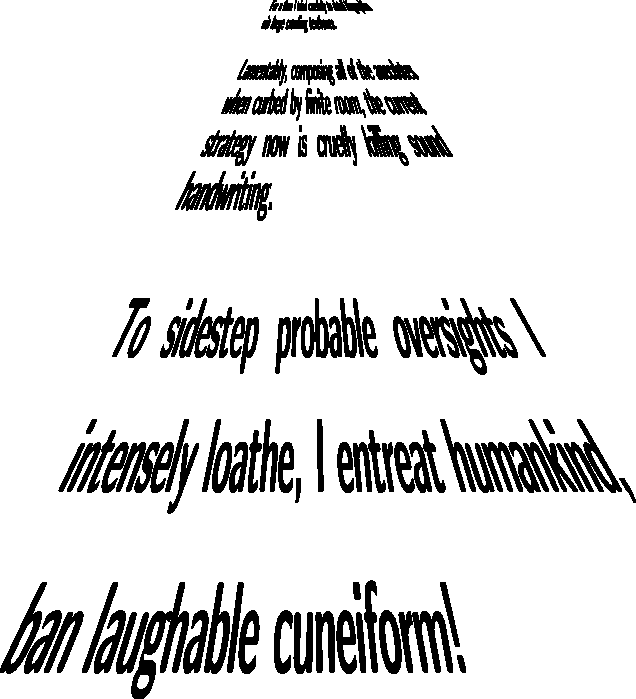
\includegraphics[width=\linewidth]{assets/star-wars-resized.pdf}
\end{center}

%For %3
%a %1
%time %4
%I %1
%tried %5
%carefully %9
%to %2
%detail %6
%biographies %B, not 5
%via %3
%large %5
%crawling %8
%textboxes. %9
%
%Lamentably, %L, not 7
%composing %9
%all %3
%of %2
%the %3
%anecdotes %A, not 8
%when %4
%curbed %6
%by %2
%finite %6
%room, %4
%the %3
%current %C, not 3
%strategy %8
%now %3
%is %2
%cruelly %7
%killing %K, not 9
%sound %5
%handwriting. %H, not 0
%
%To %2
%sidestep %8
%probable %8
%oversights %O, not 4
%I %1
%intensely %9
%loathe, %L, not 7
%I %1
%entreat %E, not 6
%humankind, %9
%ban %3
%laughable %9
%cuneiform! %9


\phChapterWorksheet{Bonus Puzzle}{Azul Puzzle}

  %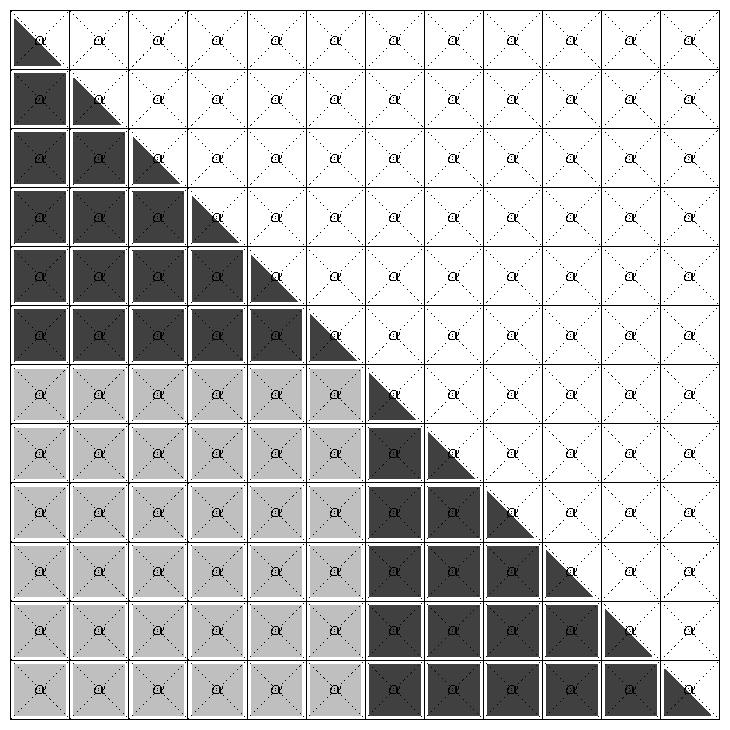
\includegraphics[width=\linewidth]{assets/wormhole-alpha}


\phChapterWorksheet{Meta Puzzle}{Alien Conversation}

  %%ASTRONAUT / PORTALS
%
%LAUNCH / PULSAR
%
%VORTEX / ORBIT
%
%GALAXY / BLACKHOLE
%
\begin{center}
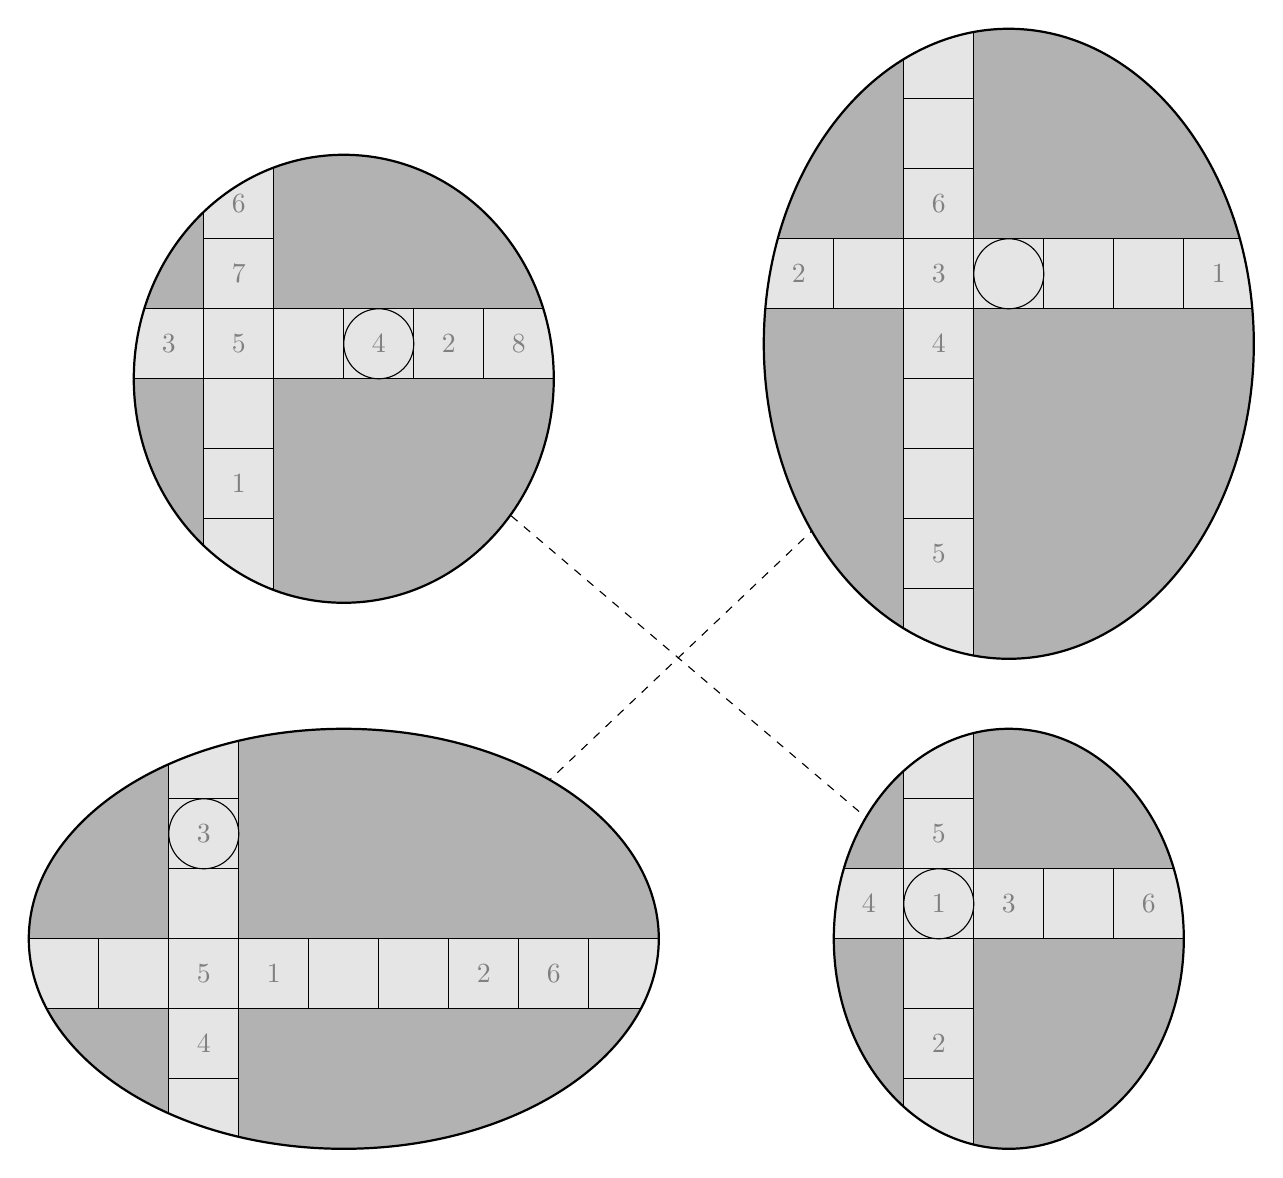
\begin{tikzpicture}[x=0.35in,y=0.35in]
\draw[dashed] (11.5,4.5) -- (1.5,-5);
\draw[dashed] (1.5,4.5) -- (11.5,-4);
\begin{scope}[shift={(10,0)}]
\begin{scope}
\clip (1.5,4.5) ellipse (3.5 and 4.5);
\fill[black!30] (-2,0) rectangle (5,9);
\fill[black!10] (0,0) rectangle (1,9);
\fill[black!10] (-2,5) rectangle (5,6);
\draw[step=1] (0,0) grid (1,9);
\draw[step=1] (-2,5) grid (5,6);
\draw (1.5,5.5) circle (0.5);
%\node[black!40] at (0.5,8.5) {A};
%\node[black!40] at (0.5,7.5) {S};
%\node[black!40] at (0.5,6.5) {T};
%\node[black!40] at (0.5,5.5) {R};
%\node[black!40] at (0.5,4.5) {O};
%\node[black!40] at (0.5,3.5) {N};
%\node[black!40] at (0.5,2.5) {A};
%\node[black!40] at (0.5,1.5) {U};
%\node[black!40] at (0.5,0.5) {T};
%\node[black!40] at (-1.5,5.5) {P};
%\node[black!40] at (-0.5,5.5) {O};
%\node[black!40] at (0.5,5.5) {R};
%\node[black!40] at (1.5,5.5) {T};
%\node[black!40] at (2.5,5.5) {A};
%\node[black!40] at (3.5,5.5) {L};
%\node[black!40] at (4.5,5.5) {S};
%SPROUT
\node[black!50] at (4.5,5.5) {1};
\node[black!50] at (-1.5,5.5) {2};
\node[black!50] at (0.5,5.5) {3};
\node[black!50] at (0.5,4.5) {4};
\node[black!50] at (0.5,1.5) {5};
\node[black!50] at (0.5,6.5) {6};
\end{scope}
\draw[thick] (1.5,4.5) ellipse (3.5 and 4.5);
\end{scope}
\begin{scope}[shift={(0,1)}]
\begin{scope}
\clip (2,3) ellipse (3 and 3.2);
\fill[black!30] (-1,-0.2) rectangle (5,6.2);
\fill[black!10] (0,0) rectangle (1,6);
\fill[black!10] (-1,3) rectangle (5,4);
\draw[step=1] (0,0) grid (1,6);
\draw[step=1] (-1,3) grid (5,4);
\draw (2.5,3.5) circle (0.5);
%\node[black!40] at (0.5,5.5) {L};
%\node[black!40] at (0.5,4.5) {A};
%\node[black!40] at (0.5,3.5) {U};
%\node[black!40] at (0.5,2.5) {N};
%\node[black!40] at (0.5,1.5) {C};
%\node[black!40] at (0.5,0.5) {H};
%\node[black!40] at (-0.5,3.5) {P};
%\node[black!40] at (0.5,3.5) {U};
%\node[black!40] at (1.5,3.5) {L};
%\node[black!40] at (2.5,3.5) {S};
%\node[black!40] at (3.5,3.5) {A};
%\node[black!40] at (4.5,3.5) {R};
%CAPSULAR
\node[black!50] at (0.5,1.5) {1};
\node[black!50] at (3.5,3.5) {2};
\node[black!50] at (-0.5,3.5) {3};
\node[black!50] at (2.5,3.5) {4};
\node[black!50] at (0.5,3.5) {5};
\node[black!50] at (0.5,5.5) {6};
\node[black!50] at (0.5,4.5) {7};
\node[black!50] at (4.5,3.5) {8};
\end{scope}
\draw[thick] (2,3) ellipse (3 and 3.2);
\end{scope}
\begin{scope}[shift={(10,-7)}]
\begin{scope}
\clip (1.5,3) ellipse (2.5 and 3);
\fill[black!30] (-1,-0.2) rectangle (5,6.2);
\fill[black!10] (0,0) rectangle (1,6);
\fill[black!10] (-1,3) rectangle (4,4);
\draw[step=1] (0,0) grid (1,6);
\draw[step=1] (-1,3) grid (5,4);
\draw (0.5,3.5) circle (0.5);
%\node[black!40] at (0.5,5.5) {V};
%\node[black!40] at (0.5,4.5) {O};
%\node[black!40] at (0.5,3.5) {R};
%\node[black!40] at (0.5,2.5) {T};
%\node[black!40] at (0.5,1.5) {E};
%\node[black!40] at (0.5,0.5) {X};
%\node[black!40] at (-0.5,3.5) {O};
%\node[black!40] at (0.5,3.5) {R};
%\node[black!40] at (1.5,3.5) {B};
%\node[black!40] at (2.5,3.5) {I};
%\node[black!40] at (3.5,3.5) {T};
%REBOOT
\node[black!50] at (0.5,3.5) {1};
\node[black!50] at (0.5,1.5) {2};
\node[black!50] at (1.5,3.5) {3};
\node[black!50] at (-0.5,3.5) {4};
\node[black!50] at (0.5,4.5) {5};
\node[black!50] at (3.5,3.5) {6};
\end{scope}
\draw[thick] (1.5,3) ellipse (2.5 and 3);
\end{scope}
\begin{scope}[shift={(-0.5,-7)}]
\begin{scope}
\clip (2.5,3) ellipse (4.5 and 3);
\fill[black!30] (-2,0) rectangle (7,6);
\fill[black!10] (0,0) rectangle (1,6);
\fill[black!10] (-2,2) rectangle (7,3);
\draw[step=1] (0,0) grid (1,6);
\draw[step=1] (-2,2) grid (7,3);
\draw (0.5,4.5) circle (0.5);
%\node[black!40] at (0.5,5.5) {G};
%\node[black!40] at (0.5,4.5) {A};
%\node[black!40] at (0.5,3.5) {L};
%\node[black!40] at (0.5,2.5) {A};
%\node[black!40] at (0.5,1.5) {X};
%\node[black!40] at (0.5,0.5) {Y};
%\node[black!40] at (-1.5,2.5) {B};
%\node[black!40] at (-0.5,2.5) {L};
%\node[black!40] at (0.5,2.5) {A};
%\node[black!40] at (1.5,2.5) {C};
%\node[black!40] at (2.5,2.5) {K};
%\node[black!40] at (3.5,2.5) {H};
%\node[black!40] at (4.5,2.5) {O};
%\node[black!40] at (5.5,2.5) {L};
%\node[black!40] at (6.5,2.5) {E};
%COAXAL
\node[black!50] at (1.5,2.5) {1};
\node[black!50] at (4.5,2.5) {2};
\node[black!50] at (0.5,4.5) {3};
\node[black!50] at (0.5,1.5) {4};
\node[black!50] at (0.5,2.5) {5};
\node[black!50] at (5.5,2.5) {6};
\end{scope}
\draw[thick] (2.5,3) ellipse (4.5 and 3);
\end{scope}
\end{tikzpicture}
\end{center}



\end{document}
